% Options for packages loaded elsewhere
\PassOptionsToPackage{unicode}{hyperref}
\PassOptionsToPackage{hyphens}{url}
\PassOptionsToPackage{dvipsnames,svgnames*,x11names*}{xcolor}
%
\documentclass[
  11pt,
  french,
]{book}
\usepackage{lmodern}
\usepackage{amssymb,amsmath}
\usepackage{ifxetex,ifluatex}
\ifnum 0\ifxetex 1\fi\ifluatex 1\fi=0 % if pdftex
  \usepackage[T1]{fontenc}
  \usepackage[utf8]{inputenc}
  \usepackage{textcomp} % provide euro and other symbols
\else % if luatex or xetex
  \usepackage{unicode-math}
  \defaultfontfeatures{Scale=MatchLowercase}
  \defaultfontfeatures[\rmfamily]{Ligatures=TeX,Scale=1}
  \setmainfont[]{Palatino Linotype}
  \setmonofont[Scale=0.8]{Source Code Pro}
\fi
% Use upquote if available, for straight quotes in verbatim environments
\IfFileExists{upquote.sty}{\usepackage{upquote}}{}
\IfFileExists{microtype.sty}{% use microtype if available
  \usepackage[]{microtype}
  \UseMicrotypeSet[protrusion]{basicmath} % disable protrusion for tt fonts
}{}
\makeatletter
\@ifundefined{KOMAClassName}{% if non-KOMA class
  \IfFileExists{parskip.sty}{%
    \usepackage{parskip}
  }{% else
    \setlength{\parindent}{0pt}
    \setlength{\parskip}{6pt plus 2pt minus 1pt}}
}{% if KOMA class
  \KOMAoptions{parskip=half}}
\makeatother
\usepackage{xcolor}
\IfFileExists{xurl.sty}{\usepackage{xurl}}{} % add URL line breaks if available
\IfFileExists{bookmark.sty}{\usepackage{bookmark}}{\usepackage{hyperref}}
\hypersetup{
  pdftitle={Méthodes quantitatives en sciences sociales avec R},
  pdfauthor={Philippe Apparicio et Jérémy Gelb},
  pdflang={fr},
  colorlinks=true,
  linkcolor=Maroon,
  filecolor=Maroon,
  citecolor=Blue,
  urlcolor=Blue,
  pdfcreator={LaTeX via pandoc}}
\urlstyle{same} % disable monospaced font for URLs
\usepackage[left=2cm,right=2cm,top=2cm,bottom=2cm]{geometry}
\usepackage{color}
\usepackage{fancyvrb}
\newcommand{\VerbBar}{|}
\newcommand{\VERB}{\Verb[commandchars=\\\{\}]}
\DefineVerbatimEnvironment{Highlighting}{Verbatim}{commandchars=\\\{\}}
% Add ',fontsize=\small' for more characters per line
\usepackage{framed}
\definecolor{shadecolor}{RGB}{248,248,248}
\newenvironment{Shaded}{\begin{snugshade}}{\end{snugshade}}
\newcommand{\AlertTok}[1]{\textcolor[rgb]{0.94,0.16,0.16}{#1}}
\newcommand{\AnnotationTok}[1]{\textcolor[rgb]{0.56,0.35,0.01}{\textbf{\textit{#1}}}}
\newcommand{\AttributeTok}[1]{\textcolor[rgb]{0.77,0.63,0.00}{#1}}
\newcommand{\BaseNTok}[1]{\textcolor[rgb]{0.00,0.00,0.81}{#1}}
\newcommand{\BuiltInTok}[1]{#1}
\newcommand{\CharTok}[1]{\textcolor[rgb]{0.31,0.60,0.02}{#1}}
\newcommand{\CommentTok}[1]{\textcolor[rgb]{0.56,0.35,0.01}{\textit{#1}}}
\newcommand{\CommentVarTok}[1]{\textcolor[rgb]{0.56,0.35,0.01}{\textbf{\textit{#1}}}}
\newcommand{\ConstantTok}[1]{\textcolor[rgb]{0.00,0.00,0.00}{#1}}
\newcommand{\ControlFlowTok}[1]{\textcolor[rgb]{0.13,0.29,0.53}{\textbf{#1}}}
\newcommand{\DataTypeTok}[1]{\textcolor[rgb]{0.13,0.29,0.53}{#1}}
\newcommand{\DecValTok}[1]{\textcolor[rgb]{0.00,0.00,0.81}{#1}}
\newcommand{\DocumentationTok}[1]{\textcolor[rgb]{0.56,0.35,0.01}{\textbf{\textit{#1}}}}
\newcommand{\ErrorTok}[1]{\textcolor[rgb]{0.64,0.00,0.00}{\textbf{#1}}}
\newcommand{\ExtensionTok}[1]{#1}
\newcommand{\FloatTok}[1]{\textcolor[rgb]{0.00,0.00,0.81}{#1}}
\newcommand{\FunctionTok}[1]{\textcolor[rgb]{0.00,0.00,0.00}{#1}}
\newcommand{\ImportTok}[1]{#1}
\newcommand{\InformationTok}[1]{\textcolor[rgb]{0.56,0.35,0.01}{\textbf{\textit{#1}}}}
\newcommand{\KeywordTok}[1]{\textcolor[rgb]{0.13,0.29,0.53}{\textbf{#1}}}
\newcommand{\NormalTok}[1]{#1}
\newcommand{\OperatorTok}[1]{\textcolor[rgb]{0.81,0.36,0.00}{\textbf{#1}}}
\newcommand{\OtherTok}[1]{\textcolor[rgb]{0.56,0.35,0.01}{#1}}
\newcommand{\PreprocessorTok}[1]{\textcolor[rgb]{0.56,0.35,0.01}{\textit{#1}}}
\newcommand{\RegionMarkerTok}[1]{#1}
\newcommand{\SpecialCharTok}[1]{\textcolor[rgb]{0.00,0.00,0.00}{#1}}
\newcommand{\SpecialStringTok}[1]{\textcolor[rgb]{0.31,0.60,0.02}{#1}}
\newcommand{\StringTok}[1]{\textcolor[rgb]{0.31,0.60,0.02}{#1}}
\newcommand{\VariableTok}[1]{\textcolor[rgb]{0.00,0.00,0.00}{#1}}
\newcommand{\VerbatimStringTok}[1]{\textcolor[rgb]{0.31,0.60,0.02}{#1}}
\newcommand{\WarningTok}[1]{\textcolor[rgb]{0.56,0.35,0.01}{\textbf{\textit{#1}}}}
\usepackage{longtable,booktabs}
% Correct order of tables after \paragraph or \subparagraph
\usepackage{etoolbox}
\makeatletter
\patchcmd\longtable{\par}{\if@noskipsec\mbox{}\fi\par}{}{}
\makeatother
% Allow footnotes in longtable head/foot
\IfFileExists{footnotehyper.sty}{\usepackage{footnotehyper}}{\usepackage{footnote}}
\makesavenoteenv{longtable}
\usepackage{graphicx,grffile}
\makeatletter
\def\maxwidth{\ifdim\Gin@nat@width>\linewidth\linewidth\else\Gin@nat@width\fi}
\def\maxheight{\ifdim\Gin@nat@height>\textheight\textheight\else\Gin@nat@height\fi}
\makeatother
% Scale images if necessary, so that they will not overflow the page
% margins by default, and it is still possible to overwrite the defaults
% using explicit options in \includegraphics[width, height, ...]{}
\setkeys{Gin}{width=\maxwidth,height=\maxheight,keepaspectratio}
% Set default figure placement to htbp
\makeatletter
\def\fps@figure{htbp}
\makeatother
\setlength{\emergencystretch}{3em} % prevent overfull lines
\providecommand{\tightlist}{%
  \setlength{\itemsep}{0pt}\setlength{\parskip}{0pt}}
\setcounter{secnumdepth}{5}
\usepackage{booktabs}
\usepackage{longtable}
\usepackage{float}
\usepackage[bf,singlelinecheck=off]{caption}
\usepackage[justification=centering]{caption}
\usepackage{fancyhdr}
\usepackage{fontspec}
\usepackage{color}

% changer la taille des en-tetes
\fancyhead{}
\fancyfoot{}
\renewcommand{\headrulewidth}{0pt}
\fancyhead[RO,LE]{\footnotesize\thepage}
\fancyhead[RE]{\footnotesize\slshape\leftmark}
\pagestyle{fancy}

\usepackage{framed,color}
\definecolor{shadecolor}{RGB}{248,248,248}
\definecolor{shadebluecolor}{RGB}{224,244,255}

\renewcommand{\textfraction}{0.05}
\renewcommand{\topfraction}{0.8}
\renewcommand{\bottomfraction}{0.8}
\renewcommand{\floatpagefraction}{0.75}

\renewenvironment{quote}{\begin{VF}}{\end{VF}}
\let\oldhref\href
\renewcommand{\href}[2]{#2\footnote{\url{#1}}}

\let\oldalign=\align
\renewcommand{\align}{\small\oldalign\normalsize}


% Creating some nice fonts
\newfontfamily{\errorfont}{Lucida Console}
\newcommand{\errorMessage}{\errorfont \color{red}}

\ifxetex
  \usepackage{letltxmacro}
  \setlength{\XeTeXLinkMargin}{1pt}
  \LetLtxMacro\SavedIncludeGraphics\includegraphics
  \def\includegraphics#1#{% #1 catches optional stuff (star/opt. arg.)
    \IncludeGraphicsAux{#1}%
  }%
  \newcommand*{\IncludeGraphicsAux}[2]{%
    \XeTeXLinkBox{%
      \SavedIncludeGraphics#1{#2}%
    }%
  }%
\fi

\makeatletter
\newenvironment{kframe}{%
\medskip{}
\setlength{\fboxsep}{.8em}
 \def\at@end@of@kframe{}%
 \ifinner\ifhmode%
  \def\at@end@of@kframe{\end{minipage}}%
  \begin{minipage}{\columnwidth}%
 \fi\fi%
 \def\FrameCommand##1{\hskip\@totalleftmargin \hskip-\fboxsep
 \colorbox{shadecolor}{##1}\hskip-\fboxsep
     % There is no \\@totalrightmargin, so:
     \hskip-\linewidth \hskip-\@totalleftmargin \hskip\columnwidth}%
 \MakeFramed {\advance\hsize-\width
   \@totalleftmargin\z@ \linewidth\hsize
   \@setminipage}}%
 {\par\unskip\endMakeFramed%
 \at@end@of@kframe}
\makeatother

\makeatletter
\newenvironment{kframev}{%
\medskip{}
\setlength{\fboxsep}{.8em}
 \def\at@end@of@kframev{}%
 \ifinner\ifhmode%
  \def\at@end@of@kframev{\end{minipage}}%
  \begin{minipage}{\columnwidth}%
 \fi\fi%
 \def\FrameCommand##1{\hskip\@totalleftmargin \hskip-\fboxsep
 \colorbox{shadebluecolor}{##1}\hskip-\fboxsep
     % There is no \\@totalrightmargin, so:
     \hskip-\linewidth \hskip-\@totalleftmargin \hskip\columnwidth}%
 \MakeFramed {\advance\hsize-\width
   \@totalleftmargin\z@ \linewidth\hsize
   \@setminipage}}%
 {\par\unskip\endMakeFramed%
 \at@end@of@kframev}
\makeatother

\renewenvironment{Shaded}{\begin{kframe}}{\end{kframe}}

\usepackage{makeidx}
\makeindex

\urlstyle{tt}

\usepackage{amsthm}
\makeatletter
\def\thm@space@setup{%
  \thm@preskip=8pt plus 2pt minus 4pt
  \thm@postskip=\thm@preskip
}

% Definition des environnements pour les blocks pdf---------------------------
\newenvironment{rmdblock}[1]
  {
  \begin{itemize}
  \renewcommand{\labelitemi}{
    \raisebox{-.7\height}[0pt][0pt]{
      {\setkeys{Gin}{width=3em,keepaspectratio}\includegraphics{images/#1}}
    }
  }
  \setlength{\fboxsep}{1em}
  \begin{kframev}
  \small
  \item
  }
  {
  \end{kframev}
  \end{itemize}
  }


\newenvironment{bloc_notes}
  {\begin{rmdblock}{notes}}
  {\end{rmdblock}}


\newenvironment{bloc_aller_loin}
  {\begin{rmdblock}{aller_loin}}
  {\end{rmdblock}}


\newenvironment{bloc_astuce}
  {\begin{rmdblock}{astuce}}
  {\end{rmdblock}}


\newenvironment{bloc_attention}
  {\begin{rmdblock}{attention}}
  {\end{rmdblock}}


\newenvironment{bloc_package}
  {\begin{rmdblock}{package}}
  {\end{rmdblock}}

\newenvironment{bloc_objectif}
  {\begin{rmdblock}{objectif}}
  {\end{rmdblock}}


% -------------------------------------------------------------------

% -------------------modifying existing environments-----------------

% changing font size of code chunks
\let\oldShaded\Shaded
\def\Shaded{\oldShaded\small}

%insuring adding a line break for level 5
\makeatletter
\renewcommand\paragraph{\@startsection{paragraph}{4}{\z@}%
   {-3.25ex\@plus -1ex \@minus -.2ex}%
   {1.5ex \@plus .2ex}%
   {\normalfont\normalsize\bfseries}}
\makeatother

% -------------------------------------------------------------------

\makeatother
\usepackage{flafter}
\usepackage{float}
\usepackage{booktabs}
\usepackage{longtable}
\usepackage{array}
\usepackage{multirow}
\usepackage{wrapfig}
\usepackage{colortbl}
\usepackage{pdflscape}
\usepackage{tabu}
\usepackage{threeparttable}
\usepackage{threeparttablex}
\usepackage[normalem]{ulem}
\usepackage{makecell}
\usepackage{xcolor}
\ifxetex
  % Load polyglossia as late as possible: uses bidi with RTL langages (e.g. Hebrew, Arabic)
  \usepackage{polyglossia}
  \setmainlanguage[]{french}
\else
  \usepackage[shorthands=off,main=french]{babel}
\fi

\title{Méthodes quantitatives en sciences sociales avec R}
\author{Philippe Apparicio et Jérémy Gelb}
\date{2022-03-19}

\begin{document}
\maketitle

%\cleardoublepage\newpage\thispagestyle{empty}\null
%\cleardoublepage\newpage\thispagestyle{empty}\null
%\cleardoublepage\newpage
%\thispagestyle{empty}
%\begin{center}
%\Large{To Jung Jae-sung (1982 -- 2018),}

%\large{a remarkably hard-working badminton player with a remarkably simple playing style}
%\includegraphics{images/dedication.pdf}
%\end{center}

%\setlength{\abovedisplayskip}{-5pt}
%\setlength{\abovedisplayshortskip}{-5pt}
% Setting the name of the lists of figures and tables
\renewcommand*\listfigurename{Liste des figures}
\renewcommand*\listtablename{Liste des tableaux}

\renewcommand*\contentsname{Table des matières}
{
\hypersetup{linkcolor=}
\setcounter{tocdepth}{2}
\tableofcontents
}
\listoftables
\listoffigures
\hypertarget{pruxe9face}{%
\chapter*{Préface}\label{pruxe9face}}
\addcontentsline{toc}{chapter}{Préface}

Ce livre vise à décrire une panoplie de méthodes quantitatives utilisées en sciences sociales avec le logiciel ouvert R. Il a d'ailleurs été écrit intégralement dans R avec \href{https://rmarkdown.rstudio.com/}{rmarkdown}. Le contenu est pensé pour être accessible à tous et toutes, même à ceux et celles n'ayant presque aucune base en statistique ou en programmation. Les personnes plus expérimentées y découvriront des sections sur des méthodes plus avancées comme les modèles à effets mixtes, les modèles multiniveaux, les modèles généralisés additifs ainsi que les méthodes factorielles et de classification. Ceux et celles souhaitant migrer progressivement d'un autre logiciel statistique vers R trouveront dans cet ouvrage les éléments pour une transition en douceur. La philosophie de ce livre est de donner toutes les clefs de compréhension et de mise en œuvre des méthodes abordées dans R. La présentation des méthodes est basée sur une approche compréhensive et intuitive plutôt que mathématique, sans pour autant que la rigueur statistique ne soit négligée. Servez-vous votre boisson chaude ou froide favorite et installez-vous dans votre meilleur fauteuil. Bonne lecture!

\hypertarget{sect001}{%
\section*{Un manuel sous la forme d'une ressource éducative libre}\label{sect001}}
\addcontentsline{toc}{section}{Un manuel sous la forme d'une ressource éducative libre}

\textbf{Pourquoi un manuel de statistique en sciences sociales sous licence libre?} Les logiciels libres sont aujourd'hui très répandus. Comparativement aux logiciels propriétaires, l'accès au code source permet à quiconque de l'utiliser, de le modifier, de le dupliquer et de le partager. Le logiciel R, dans lequel sont mises en œuvre les méthodes quantitatives décrites dans ce livre, est d'ailleurs à la fois un langage de programmation et un logiciel libre (sous la licence publique générale \href{https://fr.wikipedia.org/wiki/Licence_publique_g\%C3\%A9n\%C3\%A9rale_GNU}{GNU GLPv2}). Par analogie aux logiciels libres, il existe aussi des \textbf{ressources éducatives libres (REL)} «~dont la licence accorde les permissions désignées par les 5R (\textbf{Retenir --- Réutiliser --- Réviser --- Remixer --- Redistribuer}) et donc permet nécessairement la modification~» (\href{https://fabriquerel.org/rel/}{\textbf{\emph{fabriqueREL}}}). La licence de ce livre, CC BY-SA (figure \ref{fig:Licence}), permet donc de~:

\begin{itemize}
\tightlist
\item
  \textbf{Retenir}, c'est-à-dire télécharger et d'imprimer gratuitement le livre. Notez qu'il aurait été plutôt surprenant d'écrire un livre payant sur un logiciel libre et donc gratuit. Aussi, nous aurions été très embarrassés que des personnes étudiantes avec des ressources financières limitées doivent payer pour avoir accès au livre, sans pour autant savoir préalablement si le contenu est réellement adapté à leurs besoins.
\item
  \textbf{Réutiliser}, c'est-à-dire utiliser la totalité ou une section du livre sans limitation et sans compensation financière. Cela permet ainsi à d'autres personnes enseignantes de l'utiliser dans le cadre d'activités pédagogiques.
\item
  \textbf{Réviser}, c'est-à-dire modifier, adapter et traduire le contenu en fonction d'un besoin pédagogique précis puisqu'aucun manuel n'est parfait, tant s'en faut! Rappelons que le livre a d'ailleurs été écrit intégralement dans R avec \href{https://rmarkdown.rstudio.com/}{rmarkdown}. Quiconque peut ainsi télécharger gratuitement le code source du livre sur \href{https://LAEQ.github.io/livre_statistique_Phil_Jere/}{github} et le modifier à sa guise (voir l'encadré intitulé \emph{Suggestions d'adaptation du manuel}).
\item
  \textbf{Remixer}, c'est-à-dire «~de combiner la ressource avec d'autres ressources dont la licence le permet aussi pour créer une nouvelle ressource intégrée~» (\href{https://fabriquerel.org/rel/}{\textbf{\emph{fabriqueREL}}}).
\item
  \textbf{Redistribuer}, c'est-à-dire distribuer en totalité ou partiellement le manuel ou une version révisée sur d'autres canaux que le site Web du livre (par exemple, sur le site Moodle de votre université ou en faire une version imprimée).
\end{itemize}

\begin{figure}

{\centering 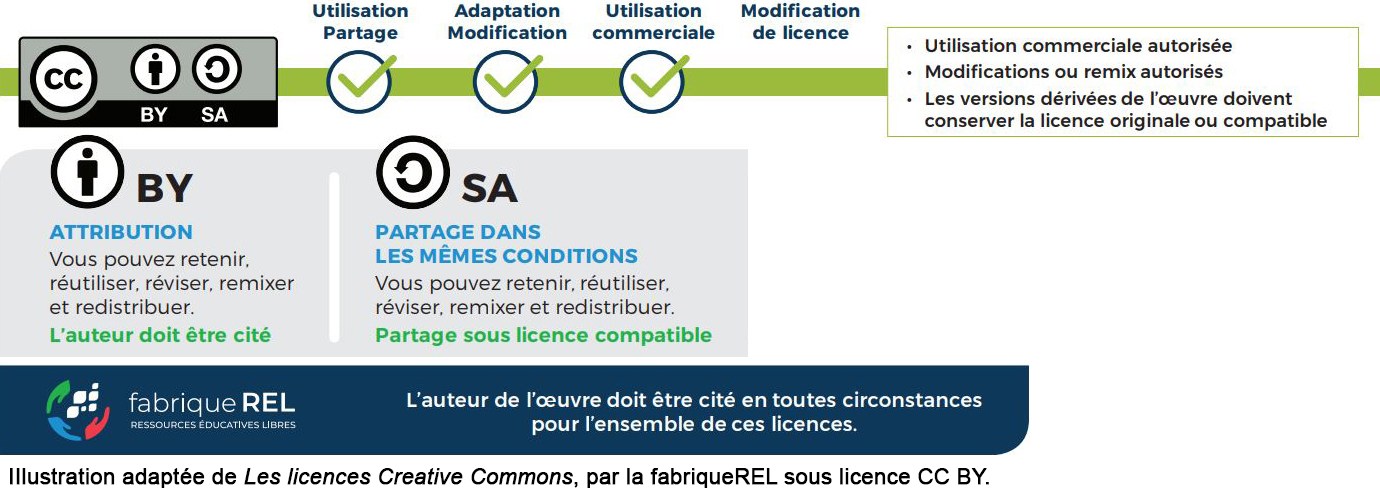
\includegraphics[width=1\linewidth]{images/Licence} 

}

\caption{Licence Creative Commons du livre}\label{fig:Licence}
\end{figure}

La licence de ce livre, CC BY-SA (figure \ref{fig:Licence}), oblige donc de~:

\begin{itemize}
\tightlist
\item
  Attribuer la paternité de l'auteur dans vos versions dérivées, ainsi qu'une mention concernant les grandes modifications apportées, en utilisant la formulation suivante~:
  Apparicio, Philippe et Jérémy Gelb. 2022. \emph{Méthodes quantitatives en sciences sociales avec R}. Institut national de la recherche scientifique. CC BY-SA (4.0).
\item
  Utiliser la même licence ou une licence similaire à toutes versions dérivées.
\end{itemize}

\begin{bloc_astuce}

\textbf{Suggestions d'adaptation du manuel}.

Notez que pour chaque méthode statistique abordée dans le livre sont disponibles une description détaillée et une mise en œuvre dans R. Par conséquent, plusieurs adaptations du manuel sont possibles~:

\begin{itemize}
\tightlist
\item
  Conserver uniquement les chapitres sur les méthodes statistiques ciblées dans votre cours.
\item
  En faire une version imprimée et la distribuer aux personnes étudiantes.
\item
  Modifier la description d'une ou plusieurs méthodes en effectuant les mises à jour directement dans les chapitres.
\item
  Insérer ses propres jeux de données dans les sections intitulées \emph{Mise en œuvre dans R}.
\item
  Modifier les tableaux et figures.
\item
  Ajouter une série d'exercices.
\item
  Rédiger un nouveau chapitre.
\item
  Modifier des syntaxes R. Plusieurs \emph{packages} R peuvent être utilisés pour mettre en œuvre telle ou telle méthode statistique. Ces derniers évoluent aussi très vite et de nouveaux \emph{packages} sont proposés fréquemment! Par conséquent, il peut être judicieux de modifier une syntaxe R du livre en fonction de ses habitudes de programmation dans R (utilisation d'autres \emph{packages} que ceux utilisés dans le manuel par exemple) ou de bien mettre à jour une syntaxe à la suite de la parution d'un nouveau \emph{package} plus performant ou intéressant.
\item
  Toute autre adaptation qui permet de répondre au mieux à un besoin pédagogique.
\end{itemize}


\end{bloc_astuce}

\hypertarget{sect002}{%
\section*{Un manuel conçu comme un projet collaboratif}\label{sect002}}
\addcontentsline{toc}{section}{Un manuel conçu comme un projet collaboratif}

Il existe actuellement de nombreux livres sous licence ouverte écrits avec \href{https://rmarkdown.rstudio.com/}{rmarkdown} avec le \emph{package} \texttt{bookdown} (Xie \protect\hyperlink{ref-xie2016bookdown}{2016}), répertoriés sur le site de \url{https://bookdown.org/}. Sans surprise, R étant un logiciel libre dédié aux méthodes statistiques et à la science des données, plusieurs abordent les méthodes quantitatives, notamment~:

\begin{itemize}
\tightlist
\item
  \href{https://bookdown.org/roback/bookdown-BeyondMLR/}{Beyond Multiple Linear Regression: Applied Generalized Linear Models and Multilevel Models in R} (Roback et Legler \protect\hyperlink{ref-roback2021beyond}{2021}), CC BY-NC-SA.
\item
  \href{https://www.econometrics-with-r.org/}{Introduction to Econometrics with R} (Hanck et al. \protect\hyperlink{ref-hanck2019introduction}{2019}), CC BY-NC-SA.
\item
  \href{https://moderndive.com/}{Statistical Inference via Data Science: A ModernDive into R and the Tidyverse} (Ismay et Kim \protect\hyperlink{ref-ismay2019statistical}{2019}), CC BY-NC-SA.
\item
  \href{https://r-graphics.org/}{R Graphics Cookbook, 2nd edition} (Chang \protect\hyperlink{ref-Chang2018}{2018}), CC BY.
\end{itemize}

Par contre, la grande majorité de ces livres numériques rédigés avec \texttt{bookdown} sont en anglais. À notre connaissance, ce projet constitue le premier manuel numérique en français sur les méthodes quantitatives appliquées aux sciences sociales réalisé avec \texttt{bookdown}. La première version du livre étant lancée, il est grand temps de planifier les suivantes! Pour ce faire, nous considérons ce livre comme un \textbf{projet collaboratif visant à mobiliser la communauté universitaire francophone qui enseigne les statistiques en sciences sociales avec R}. Plusieurs raisons motivent cette vision collaborative~:

\begin{itemize}
\tightlist
\item
  \textbf{Rien n'est parfait!} Cette première version comprend sûrement des coquilles et certaines sections mériteraient d'être améliorées. Les commentaires et suggestions visant à améliorer son contenu sont les bienvenus.
\item
  \textbf{La table des matières doit être impérativement extensible!} De nombreuses méthodes statistiques très utilisées en sciences sociales ne sont pas abordées dans ce livre et mériteraient d'être ajoutées dans une version ultérieure~: certaines extensions des régressions linéaires (régressions Rigge et Lasso, Tobit, quantile, etc.), les modèles d'équations simultanées, les analyses de données longitudinales (entre autres, modèles de survie, régression par panel), les modèles d'équations structurelles et bien d'autres! Par conséquent, si vous êtes intéressé(e)s, à ajouter un nouveau chapitre ou une partie du livre, nous vous invitons vivement à communiquer avec nous ou à diffuser sous une licence similaire votre version dérivée. L'objectif étant de continuer à faire tourner la roue du libre et, idéalement, que les futures versions soient corédigées par une communauté d'auteurs et d'autrices spécialistes en méthodes quantitatives.
\end{itemize}

\hypertarget{sect003}{%
\section*{Comment lire ce livre?}\label{sect003}}
\addcontentsline{toc}{section}{Comment lire ce livre?}

Si vous googlez l'expression «~comment lire un livre?~», vous trouverez une multitude de conseils et astuces. Pour ce livre, nous vous conseillons de le lire de gauche à droite et page par page! Plus sérieusement, le livre comprend plusieurs types de blocs de texte qui, nous l'espèrons, en facilitent la lecture.

\begin{bloc_package}
\textbf{Bloc \emph{packages}}. Habituellement localisé au début d'un chapitre, il comprend la liste des \emph{packages} R utilisés pour un chapitre.

\end{bloc_package}

\begin{bloc_objectif}
\textbf{Bloc objectif}. Il comprend une description des objectifs d'un chapitre ou d'une section.

\end{bloc_objectif}

\begin{bloc_notes}
\textbf{Bloc notes}. Il comprend une information secondaire sur une notion, un élément, une idée abordée dans une section.

\end{bloc_notes}

\begin{bloc_aller_loin}
\textbf{Bloc pour aller plus loin}. Il comprend des références ou des extensions d'une méthode statistique abordée dans une section.

\end{bloc_aller_loin}

\begin{bloc_astuce}
\textbf{Bloc astuce}. Il décrit un élément qui vous facilitera le vie~: une propriété statistique, un \emph{package}, une fonction, une syntaxe R.

\end{bloc_astuce}

\begin{bloc_attention}
\textbf{Bloc attention}. Il comprend une notion ou un élément important à bien maîtriser.

\end{bloc_attention}

\hypertarget{sect003B}{%
\section*{Comment utiliser les données du livre pour reproduire les exemples?}\label{sect003B}}
\addcontentsline{toc}{section}{Comment utiliser les données du livre pour reproduire les exemples?}

Ce livre propose des exemples détaillés et appliqués dans R pour chacune des méthodes abordées. Ces exemples se basent sur des jeux de données structurés et mis à disposition avec le livre. Ils sont disponibles sur le \emph{repo github} dans le sous-dossier \texttt{data}, à l'adresse \url{https://github.com/LAEQ/livre_statistique_Phil_Jere/tree/master/data}.

Pour télécharger l'intégralité des données, vous pouvez utiliser le lien suivant~: \url{https://downgit.github.io/\#/home?url=https://github.com/LAEQ/livre_statistique_Phil_Jere/tree/master/data}. Cela est rendu possible grâce à l'outil \href{https://downgit.github.io/\#/home}{DownGit}.

Une autre option est de télécharger le \emph{repo} complet du livre directement sur \emph{github} (\url{https://github.com/LAEQ/livre_statistique_Phil_Jere}) en cliquant sur le bouton \texttt{Code}, puis le bouton \texttt{Download\ ZIP} (figure \ref{fig:downloaffromgit}). Les données se trouvent alors dans le sous-dossier nommé \texttt{data}.

\begin{figure}

{\centering 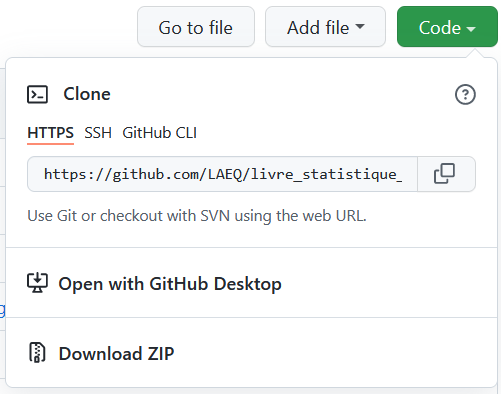
\includegraphics[width=0.5\linewidth]{images/introduction/download_github} 

}

\caption{Téléchargement de l'intégralité du livre}\label{fig:downloaffromgit}
\end{figure}

\hypertarget{sect004}{%
\section*{Structure du livre}\label{sect004}}
\addcontentsline{toc}{section}{Structure du livre}

Le livre est organisé autour de cinq grandes parties.

\textbf{Partie 1. La découverte de R.} Dans cette première partie, nous discutons brièvement de l'histoire et de la philosophie de R. Nous voyons ensuite comment installer R et RStudio. Les bases du langage R (particulièrement les principaux objets que sont le vecteur, la matrice, la liste et le \emph{dataframe}) ainsi que la manipulation des données avec R sont aussi largement abordés dans le chapitre \ref{chap01}.

\textbf{Partie 2. Analyses univariées et représentations graphiques}. Cette seconde partie comprend deux chapitres. Dans le chapitre \ref{chap02}, nous décrivons dans un premier temps les différents types de données (primaires \emph{versus} secondaires, transversales \emph{versus} longitudinales, spatiales \emph{versus} aspatiales, individuelles \emph{versus} agrégées), les différents types de variables quantitatives (discrètes et continues) et qualitatives (nominales et ordinales) et les principales distributions de variables utilisées en sciences sociales (uniforme, Bernoulli, binomiale, géométrique, binomiale négative, poisson, poisson avec excès de zéros, gaussienne, gaussienne asymétrique, log-normale, Student, Cauchy, Chi-carré, exponentielle, gamma, bêta, Weibull et Pareto). Dans un second temps, nous abordons les statistiques descriptives pour des variables quantitatives (paramètres de tendance centrale, paramètres de position, paramètres de dispersion, paramètres de forme), puis qualitatives (fréquences absolues, relatives et cumulées).

Dans le chapitre \ref{chap03}, nous illustrons les incroyables capacités graphiques de R en mettant en œuvre les principaux graphiques (histogramme, graphique de densité, nuage de points, graphique en lignes, boîtes à moustache, graphique en violon, graphique en barre, graphique circulaire), quelques graphiques particuliers (graphique en radar, diagramme d'accord, nuage de mots, carte proportionnelle) et une initiation aux cartes choroplèthes.

\textbf{Partie 3. Analyses bivariées.} Cette troisième partie comprend trois chapitres dans lesquelles sont présentées les principales méthodes exploratoires et confirmatoires bivariées permettant d'évaluer la relation entre deux variables. Plus spécifiquement, nous présentons puis mettons en œuvre dans R les méthodes permettant d'explorer les relations entre deux variables quantitatives (covariance, corrélation et régression linéaire simple) dans le chapitre \ref{chap04}, deux variables qualitatives (tableau de contingence et test du khi-deux) dans le chapitre \ref{chap05} et une variable quantitative avec une variable qualitative avec deux modalités (tests de Student, de Welch et de Wilcoxon) ou avec plus de deux modalités (ANOVA et test de Kruskal-Wallis) dans le chapitre \ref{chap06}.

\textbf{Partie 4. Modèles de régression}. Dans cette quatrième partie, sont présentées les principales méthodes de statistique inférentielle utilisées en sciences sociales~: la régression linéaire multiple (chapitre \ref{chap07}), les régressions linéaires généralisées (chapitre \ref{chap08}), les régressions à effets mixtes (chapitre \ref{chap09}), les régressions à effets mixtes (chapitre \ref{chap10}), les régressions multiniveaux (chapitre \ref{chap11}) et les modèles généralisés additifs (chapitre \ref{chap12}).

\textbf{Partie 5. Analyses exploratoires multivariées}. Dans cette cinquième partie, sont abordées les méthodes de statistique exploratoire et descriptive permettant de décrire des tableaux de données comprenant plusieurs variables. Nous décrivons d'abord les méthodes de réduction de données~: les méthodes factorielles dans le chapitre \ref{chap12} (analyses de composantes principales, analyses factorielles de correspondances, analyses factorielles de correspondances multiples) et les méthodes de classification non supervisées dans le chapitre \ref{chap13} (classification ascendante hiérarchique, k-moyennes, k-médianes, k-médoïdes et leurs extensions en logique floue comme les c-moyennes et c-médianes).

\hypertarget{sect005}{%
\section*{Pourquoi faut-il programmer en sciences sociales?}\label{sect005}}
\addcontentsline{toc}{section}{Pourquoi faut-il programmer en sciences sociales?}

Vous contrasterez rapidement que R est un véritable langage de programmation. L'apprentissage de ce language de programmation est-il pour autant pertinent pour les étudiants et étudiantes en sciences sociales? Il est vrai que la programmation n'est pas une compétence qui vient d'emblée à l'esprit lorsque l'on s'intéresse à la recherche aux sciences sociales. Pourtant, elle est de plus en plus importante, et ce, pour plusieurs raisons~:

\begin{itemize}
\tightlist
\item
  Une part toujours plus grande des phénomènes sociaux se produisent ou peuvent s'observer au travers d'environnements numériques. Être capable d'exploiter efficacement ces outils permet d'extraire des données riches sur des phénomènes complexes, tel qu'en témoignent des études récentes sur la propagation de la désinformation sur les réseaux sociaux (Allcott et Gentzkow \protect\hyperlink{ref-allcott2017social}{2017}), la migration des personnes (Spyratos et al. \protect\hyperlink{ref-spyratos2019quantifying}{2019}), la propagation et les risques de contamination de la COVID-19 (Boulos et Geraghty \protect\hyperlink{ref-boulos2020geographical}{2020}). Le plus souvent, les interfaces (API par exemple) permettant d'accéder à ces données nécessitent des habiletés en programmation.
\item
  La quantité de données numériques ouvertes et accessibles en ligne croit chaque année sur des sujets très divers. La plupart des villes et des gouvernements ont maintenant leur portail de données ouvertes auxquelles s'ajoutent les données produites par des projets collaboratifs comme \href{https://www.openstreetmap.org}{OpenStreetMap} ou \href{https://noise-planet.org/map_noisecapture/index.html}{NoisePlanet}. Récupérer ces données et les structurer pour les utiliser à des fins de recherche nécessitent le plus souvent des compétences en programmation.
\item
  Les méthodes quantitatives connaissent également un développement très important. Les logiciels propriétaires peinent à suivre la cadence de ce développement, contrairement aux logiciels à code source ouvert (comme R) qui permettent d'avoir accès aux dernières méthodes. Il est souvent long et coûteux de développer une interface graphique pour un logiciel, ce qui explique que la plupart de ces programmes en sont dépourvus et nécessitent alors de savoir programmer pour les utiliser.
\item
  Savoir programmer donne une liberté considérable en recherche. Cette compétence permet notamment de ne plus être limité(e) aux fonctionnalités proposées par des logiciels spécifiques. Il devient possible d'innover tant en matière de structuration, d'exploration et d'analyse des données que de représentation des résultats en écrivant ses propres fonctions. Cette flexibilité contribue directement à la production d'une recherche de meilleure qualité et plus diversifiée.
\item
  Programmer permet également d'automatiser des tâches qui autrement seraient extrêmement répétitives comme~: déplacer et renommer une centaine de fichiers; retirer les lignes inutiles dans un ensemble de fichiers et les compiler dans une seule base de données; vérifier parmi des milliers d'adresses lesquelles sont valides; récupérer chaque jour les messages postés sur un forum. Autant de tâches faciles à automatiser si l'on sait programmer.
\item
  Dans un logiciel avec une interface graphique, il est compliqué de conserver un historique des opérations effectuées. Programmer permet au contraire de garder une trace de l'ensemble des actions effectuées au cours d'un projet de recherche. En effet, le code utilisé reste disponible et permet de reproduire (ou d'adapter) la méthode et les résultats obtenus, ce qui est essentiel dans le monde de la recherche. À cela s'ajoute le fait que chaque ligne de code que vous écrivez vient s'ajouter à un capital de code que vous possédez, car elles pourront être réutilisées dans d'autres projets!
\end{itemize}

\hypertarget{sect006}{%
\section*{Remerciements}\label{sect006}}
\addcontentsline{toc}{section}{Remerciements}

De nombreuses personnes ont contribué à l'élaboration de ce manuel. Ce projet a bénéficié du soutien pédagogique et financier de la \href{https://fabriquerel.org/}{\textbf{\emph{fabriqueREL}}} (ressources éducatives libres). Les différentes rencontres avec le comité de suivi nous ont permis de comprendre l'univers des ressources éducatives libres (REL) et notamment leurs \href{https://fabriquerel.org/rel/}{fameux 5R} (Retenir --- Réutiliser --- Réviser --- Remixer --- Redistribuer), de mieux définir le besoin pédagogique visé par ce manuel, d'identifier des outils et des ressources pédagogiques pertinents pour son élaboration. Ainsi, nous remercions chaleureusement les membres de suivi de la \emph{fabriqueREL} pour leur support inconditionnel~:

\begin{itemize}
\tightlist
\item
  Myriam Beaudet, bibliothécaire à l'Université de Sherbrooke.
\item
  Marianne Dubé, conseillère pédagogique à l'Université de Sherbrooke et coordonnatrice de la fabriqueREL.
\item
  Myrian Grondin, bibliothécaire à l'Institut national de la recherche scientifique (INRS).
\item
  Claude Potvin, conseiller en formation à l'Université Laval.
\item
  Serge Allary, vice-recteur adjoint aux études de l'Université de Sherbrooke.
\end{itemize}

Nous tenons aussi à remercier sincèrement les étudiants et étudiantes du cours \textbf{Méthodes quantitatives appliquées aux études urbaines (EUR8219)} du programme de maîtrise en études urbaines de l'INRS. Leurs commentaires et suggestions nous ont permis d'améliorer grandement les versions préliminaires de ce manuel qui ont été utilisées dans le cadre de ce cours.

Nous remercions les membres du comité de révision pour leurs commentaires et suggestions très constructifs. Ce comité est composé de trois étudiantes et deux professeurs de l'\href{https://inrs.ca/}{INRS}~:

\begin{itemize}
\tightlist
\item
  Victoria Gay-Gauvin, étudiante à la maîtrise en études urbaines.
\item
  Salomé Vallette, étudiante au doctorat en études urbaines.
\item
  Diana Pena Ruiz, étudiante au doctorat en études des populations.
\item
  \href{https://inrs.ca/la-recherche/professeurs/benoit-laplante/}{Benoît Laplante}, professeur enseignant aux programmes de maîtrise et de doctorat en études des populations.
\item
  \href{https://inrs.ca/la-recherche/professeurs/xavier-leloup/}{Xavier Leloup}, professeur enseignant au programme de doctorat en études urbaines.
\end{itemize}

Finalement, nous remercions Denise Latreille, réviseure linguistique et chargée de cours à l'Université Sherbrooke, pour la révision du manuel.

\hypertarget{sect007}{%
\section*{Dédicace toute spéciale à Cargo et Ambrée}\label{sect007}}
\addcontentsline{toc}{section}{Dédicace toute spéciale à Cargo et Ambrée}

Fait cocasse, l'écriture de ce livre a démarré lorsque Philippe Apparicio était famille d'accueil d'un chiot de la \href{https://www.mira.ca/fr/}{Fondation Mira}, un organisme à but non lucratif qui forme des chiens-guides et d'assistance pour accroître l'autonomie et l'inclusion sociale des personnes vivant avec un handicap visuel ou moteur, ainsi que des jeunes présentant un trouble du spectre de l'autisme (TSA). En fin de rédaction du livre, ce fût au tour de Jérémy Gelb d'être famille d'accueil d'un autre chiot Mira. Nous remercions chaleureusement la \href{https://www.mira.ca/fr/}{Fondation Mira} pour nous avoir donné l'occasion de vivre cette expérience incroyable. Ce livre est donc dédié au beau Cargo et à la belle Ambrée qui nous ont tant supportés dans l'écriture du livre. Il n'y a rien de plus relaxant que d'écrire un livre de statistique avec un chiot qui dort à ses pieds!

\begin{figure}

{\centering 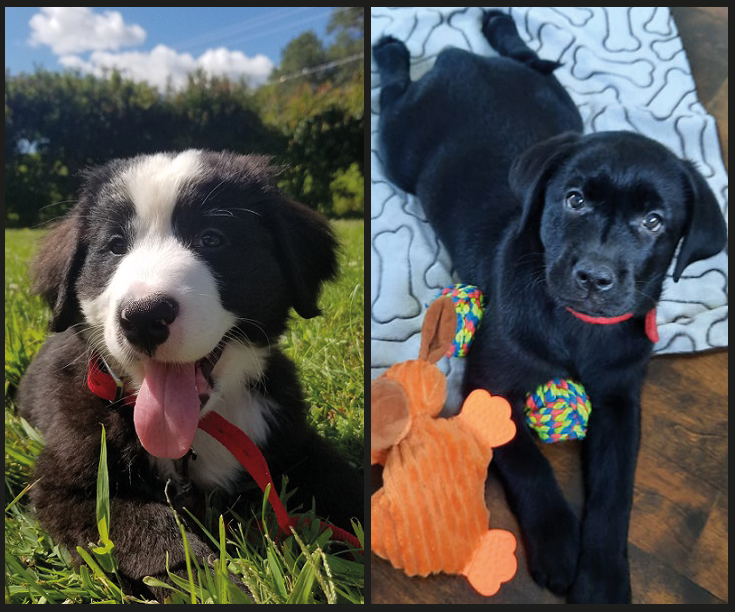
\includegraphics[width=0.7\linewidth]{images/CargoAmbre} 

}

\caption{Cargo et Ambrée, chiots de la Fondation Mira}\label{fig:CargoAmbre}
\end{figure}

\hypertarget{part-analyses-exploratoires-multivariuxe9es}{%
\part{Analyses exploratoires multivariées}\label{part-analyses-exploratoires-multivariuxe9es}}

\hypertarget{chap12}{%
\chapter{Méthodes factorielles}\label{chap12}}

\begin{bloc_attention}
Ce chapitre n'a pas encore fait l'objet d'une révision linguistique. Il comprend certainement plusieurs coquilles\ldots{} Une version révisée sera mise à jour prochainement.

\end{bloc_attention}

Dans le cadre de ce chapitre, nous présentons les trois méthodes factorielles les plus utilisées en sciences sociales~: l'analyse en composantes principales (ACP, section \ref{sect122}), l'analyse factorielle des correspondances (AFC, section \ref{sect123}) et l'analyse factorielle des correspondances multiples (ACM, section \ref{sect124}). Ces méthodes qui permettent d'explorer et de synthétiser l'information de différents tableaux de données relèvent de la statistique exploratoire multidimensionnelle.

\begin{bloc_package}

Dans ce chapitre, nous utilisons principalement les \emph{packages} suivants~:

\begin{itemize}
\tightlist
\item
  Pour créer des graphiques~:

  \begin{itemize}
  \tightlist
  \item
    \texttt{ggplot2}, le seul, l'unique!
  \item
    \texttt{ggpubr} pour combiner des graphiques.
  \end{itemize}
\item
  Pour les analyses factorielles~:

  \begin{itemize}
  \tightlist
  \item
    \texttt{FactoMineR} pour réaliser des ACP, AFC et ACM.
  \item
    \texttt{factoextra} pour réaliser des graphiques à partir des résultats d'une analyse factorielle.
  \item
    \texttt{explor} pour les résultats d'une ACP, d'une AFC ou d'une ACM avec une interface Web interactive.
  \end{itemize}
\item
  Autre \emph{package}~:

  \begin{itemize}
  \tightlist
  \item
    \texttt{geocmeans} pour un jeu de données utilisé pour calculer une ACP.
  \item
    \texttt{ggplot2}, \texttt{ggpubr}, \texttt{stringr} et \texttt{corrplot} pour réaliser des graphiques personnalisés sur les résultats d'une analyse factorielle.
  \item
    \texttt{tmap} et \texttt{RColorBrewer} pour cartographier les coordonnées factorielles.
  \item
    \texttt{Hmisc} pour l'obtention d'une matrice de corrélation.
  \end{itemize}
\end{itemize}


\end{bloc_package}

\begin{bloc_objectif}
\textbf{Réduction de données et identification de variables latentes}

Les méthodes factorielles sont souvent dénommées des \textbf{méthodes de réduction de données}, en raison de leur objectif principal, à savoir résumer l'information d'un tableau en de nouvelles variables synthétiques (figure~\ref{fig:AnalysesFactoriellesFig}). Ainsi, elles permettent de réduire l'information d'un tableau volumineux ---~comprenant par exemple 1000~observations et 100~variables~--- en \emph{p} nouvelles variables (par exemple cinq avec toujours 1000~observations) résumant \emph{X} \% de l'information contenue dans le tableau initial. Formulée plus mathématiquement, Lebart et al.~(\protect\hyperlink{ref-lebart1995statistique}{1995}, pp.~13) signalent qu'avec les méthodes factorielles, «~on cherche à réduire les dimensions du tableau de données en représentant les associations entre individus et entre variables dans des espaces de faibles dimensions~».

\begin{figure}[H]

{\centering 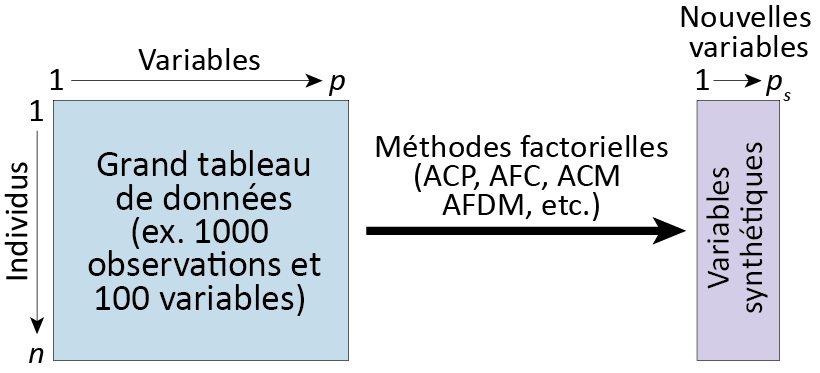
\includegraphics[width=0.5\linewidth]{images/analysesfactorielles/AnalysesFactorielles} 

}

\caption{Principe de base des analyses factorielles}\label{fig:AnalysesFactoriellesFig}
\end{figure}

Ces nouvelles variables synthétiques peuvent être considérées comme des \textbf{variables latentes} puisqu'elles ne sont directement observées, mais plutôt produites par la méthode factorielle utilisée afin de résumer les relations/associations entre plusieurs variables mesurées initialement.

\end{bloc_objectif}

\hypertarget{sect121}{%
\section{Aperçu des méthodes factorielles}\label{sect121}}

\hypertarget{sect1211}{%
\subsection{Méthodes factorielles et types de données}\label{sect1211}}

En analyse factorielle, la nature même des données du tableau à traiter détermine la méthode à employer~: l'analyse en composantes principales (ACP) est adaptée aux tableaux avec des variables continues (idéalement normalement distribuées), l'analyse factorielle des correspondances (AFC) s'applique à des tableaux de contingence tandis que l'analyse des correspondances multiples (ACM) permet de résumer des tableaux avec des données qualitatives (issues d'un sondage par exemple) (tableau~\ref{tab:typesanalysesfactorielles}). Sachez toutefois qu'il existe d'autres méthodes factorielles qui ne sont pas abordées dans ce chapitre, notamment~: l'analyse factorielle de données mixtes (AFDM) permettant d'explorer des tableaux avec à la fois des variables continues et des variables qualitatives, l'analyse factorielle multiple hiérarchique (AFMH) permettant de traiter des tableaux avec une structure hiérarchique. Pour s'initier à ces deux autres méthodes factorielles plus récentes, consultez notamment l'excellent ouvrage de Jérôme Pagès (\protect\hyperlink{ref-pages2013analyse}{2013}).

\begin{table}

\caption{\label{tab:typesanalysesfactorielles}Trois principales méthodes factorielles}
\centering
\fontsize{8}{10}\selectfont
\begin{tabular}[t]{llll}
\toprule
Méthode factorielle & Abr. & Type de données & Type de distance\\
\midrule
Analyse en composantes principales & ACP & Variables continues & Distance euclidienne\\
Analyse factorielle des correspondances & AFC & Tableau de contingence & Distance du khi-deux\\
Analyse factorielle des correspondances multiples & ACM & Variables qualitatives & Distance du khi-deux\\
\bottomrule
\end{tabular}
\end{table}

\hypertarget{sect1212}{%
\subsection{Bref historique des méthodes factorielles}\label{sect1212}}

Il existe une longue tradition de l'utilisation des méthodes factorielles dans le monde universitaire francophone puisque plusieurs d'entre elles ont été proposées par des statisticiens et des statisticiennes francophones à partir des années 1960. L'analyse en composantes principales (ACP) a été proposée dès les années 1930 par le statisticien américain Harold Hotelling (\protect\hyperlink{ref-hotelling1933analysis}{1933}). En revanche, l'analyse des correspondances (AFC) et son extension (l'analyse des correspondances multiples, ACM) ont été proposées par le statisticien français Jean-Paul Benzécri (\protect\hyperlink{ref-benzecri1973analyse}{1973}), tandis que l'analyse factorielle de données mixtes (AFDM) a été proposée par Brigitte Escofier et Jérôme Pagès (Escofier \protect\hyperlink{ref-escofier1979traitement}{1979}; Pagès \protect\hyperlink{ref-pages2002analyse}{2002}).

Ainsi, plusieurs ouvrages de statistique sur les méthodes factorielles, désormais classiques, ont été publiés en français (Benzécri \protect\hyperlink{ref-benzecri1973analyse}{1973}; Escofier et Pagès \protect\hyperlink{ref-escofier1998analyses}{1998}; Lebart, Morineau et Piron \protect\hyperlink{ref-lebart1995statistique}{1995}; Pagès \protect\hyperlink{ref-pages2013analyse}{2013}). Ils méritent grandement d'être consultés, notamment pour mieux comprendre les formulations mathématiques (matricielles et géométriques) de ces méthodes. À cela, s'ajoutent plusieurs ouvrages visant à «~vulgariser ces méthodes~» en sciences sociales; c'est notamment le cas de l'excellent ouvrage de Léna Sanders (\protect\hyperlink{ref-sanders1989analyse}{1989}) en géographie.

\hypertarget{sect122}{%
\section{Analyses en composantes principales (ACP)}\label{sect122}}

D'emblée, notez qu'il existe deux types d'analyse en composantes principales (ACP) (\emph{Principal Component Analysis, PCA} en anglais)~:

\begin{itemize}
\tightlist
\item
  \textbf{l'ACP non normée} dans laquelle les variables quantitatives du tableau sont uniquement centrées (moyenne~=~0).
\item
  \textbf{l'ACP normée} dans laquelle les variables quantitatives du tableau sont préalablement centrées réduites (moyenne~=~0 et variance~=~1; section \ref{sect02552}).
\end{itemize}

Puisque les variables d'un tableau sont souvent exprimées dans des unités de mesure différentes ou avec des ordres de grandeur différents (intervalles et écarts-types bien différents), l'utilisation de l'ACP normée est bien plus courante. Elle est d'ailleurs l'option par défaut dans les fonctions R permettant de calculer une ACP. Par conséquent, nous détaillons dans cette section uniquement l'ACP normée.

Autrement dit, le recours à une ACP non normée est plus rare et s'applique uniquement à la situation suivante~: toutes les variables du tableau sont mesurées dans la même unité (par exemple, en pourcentage); il pourrait être ainsi judicieux de conserver leurs variances respectives.

\hypertarget{sect1221}{%
\subsection{Recherche d'une simplification}\label{sect1221}}

L'ACP permet d'explorer et de résumer un tableau constitué uniquement de variables quantitatives (figure~\ref{fig:AnalysesFactoriellesTabACPFig}), et ce, de trois façons~: 1) en montrant les ressemblances entre les individus (observations), 2) en révélant les liaisons entre les variables quantitatives et 3) en résumant l'ensemble des variables du tableau par des variables synthétiques nommées composantes principales.

\begin{figure}

{\centering 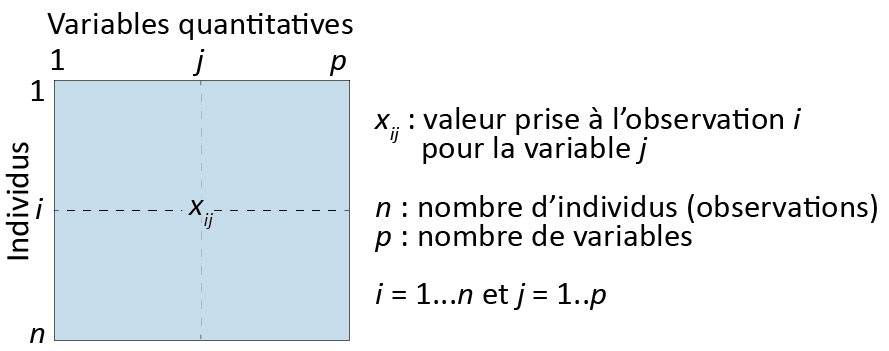
\includegraphics[width=0.6\linewidth]{images/analysesfactorielles/AnalysesFactoriellesTabACP} 

}

\caption{Tableau pour une ACP}\label{fig:AnalysesFactoriellesTabACPFig}
\end{figure}

\textbf{Ressemblance entre les individus}. Concrètement deux individus se ressemblent si leurs valeurs respectives pour les \emph{p} variables du tableau sont similaires. Cette proximité/ressemblance est évaluée à partir de la distance euclidienne~ (eq. \eqref{eq:ACPdistEuc}). La notion de distance fait l'objet d'une section à part entière (section \ref{classifDistance}) que vous pouvez consulter dès à présent si elle ne vous est pas familière.

\footnotesize

\begin{equation}
d^2(a,b) = \sum_{j=1}^p(x_{aj}-x_{bj})^2
\label{eq:ACPdistEuc}
\end{equation}
\normalsize

Prenons un exemple fictif avec trois individus (\emph{i}, \emph{j} et \emph{k}) ayant des valeurs pour trois variables préalablement centrées réduites (V1 à V3) (tableau~\ref{tab:distanceACPindi}). La proximité entre les paires de points est évaluée comme suit~:

\(d^2(i,j)=(-\mbox{1,15}-\mbox{0,49})^2+(-\mbox{1,15}-\mbox{0,58})^2+(\mbox{0,83}+\mbox{1,11})^2=\mbox{9,44}\)
\(d^2(i,k)=(-\mbox{1,15}+\mbox{0,66})^2+(-\mbox{1,15}-\mbox{0,58})^2+(\mbox{0,83}-\mbox{0,28})^2=\mbox{5,98}\)
\(d^2(j,k)= (\mbox{0,49}+\mbox{0,66})^2+(\mbox{0,58}-\mbox{0,58})^2+(-\mbox{1,11}-\mbox{0,28})^2=\mbox{1,97}\)

Nous pouvons en conclure que \emph{i} est plus proche de \emph{k} que de \emph{j}, mais aussi que la paire de points les plus proches est (\emph{i},\emph{k}). En d'autres termes, les deux observations \emph{i} et \emph{k} sont les plus similaires du jeu de données selon la distance euclidienne.

\begin{table}

\caption{\label{tab:distanceACPindi}Données fictives}
\centering
\fontsize{8}{10}\selectfont
\begin{tabular}[t]{cccc}
\toprule
\multicolumn{1}{c}{ } & \multicolumn{3}{c}{Variables centrées réduites} \\
\cmidrule(l{3pt}r{3pt}){2-4}
Individu & V1 & V2 & V3\\
\midrule
i & -1,15 & -1,15 & 0,83\\
j & 0,49 & 0,58 & -1,11\\
k & 0,66 & 0,58 & 0,28\\
\bottomrule
\end{tabular}
\end{table}

\textbf{Liaisons entre les variables}. Dans une ACP normée, les liaisons entre les variables deux à deux sont évaluées avec le coefficient de corrélation (section \ref{sect0431}), soit la moyenne du produit des deux variables centrées réduites (eq. \eqref{eq:ACPcor}). Notez que dans une ACP non normée, plus rarement utilisée, les liaisons sont alors évaluées avec la covariance puisque les variables sont uniquement centrées (eq. \eqref{eq:ACPcov}).

\footnotesize

\begin{equation}
r_{xy} = \frac{\sum_{i=1}^n (x_{i}-\bar{x})(y_{i}-\bar{y})}{n\sqrt{\sum_{i=1}^n(x_i - \bar{x})^2(y_i - \bar{y})^2}}=\sum_{i=1}^n\frac{Zx_iZy_i}{n}
\label{eq:ACPcor}
\end{equation}
\normalsize

\footnotesize

\begin{equation}
cov(x,y) = \frac{\sum_{i=1}^n (x_{i}-\bar{x})(y_{i}-\bar{y})}{n}
\label{eq:ACPcov}
\end{equation}
\normalsize

\textbf{Composantes principales}. Au chapitre~4, nous avons abordé deux méthodes pour identifier des relations linéaires entre des variables continues normalement distribuées~:

\begin{itemize}
\tightlist
\item
  la corrélation de Pearson (section \ref{sect043}), qu'il est possible d'illustrer graphiquement à partir d'un nuage de points;
\item
  la régression linéaire simple (section \ref{sect044}), permettant de résumer la relation linéaire entre deux variables avec une droite de régression de type \(Y=a+bX\).
\end{itemize}

Brièvement, plus deux variables sont corrélées (positivement ou négativement), plus le nuage de points qu'elles forment est allongé et plus les points sont proches de la droite de régression (figure~\ref{fig:liaisons2Vars}, partie~\textbf{a}). À l'inverse, plus la liaison entre les deux variables normalement distribuées est faible, plus le nuage prend la forme d'un cercle et plus les points du nuage sont éloignés de la droite de régression (figure~\ref{fig:liaisons2Vars}, partie~\textbf{b}). Puisqu'en ACP normée, les variables sont centrées réduites, le centre de gravité du nuage de points est (\emph{x}=0, \emph{y}=0) et il est toujours traversé par la droite de régression. Finalement, nous avons vu que la méthode des moindres carrés ordinaires (MCO) permet de déterminer cette droite en minimisant les distances entre les valeurs observées et celles projetées orthogonalement sur cette droite (valeurs prédites). Dans le cas de deux variables uniquement, l'axe factoriel principal/la composante principale est donc la droite qui résume le mieux la liaison entre les deux variables (en rouge). L'axe 2~ représente la seconde plus importante composante (axe, dimension) et il est orthogonal (perpendiculaire) au premier axe.

\begin{figure}

{\centering 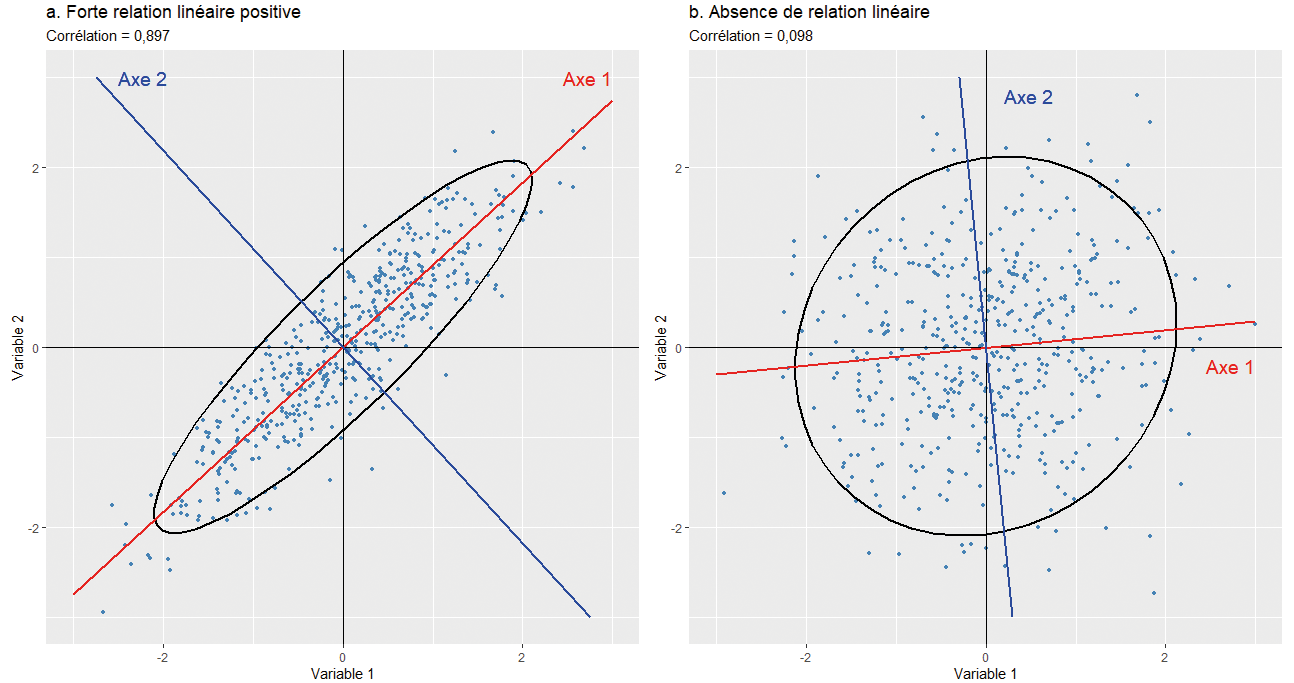
\includegraphics[width=1\linewidth]{images/analysesfactorielles/bivariePlanFacto} 

}

\caption{Corrélation, allongement du nuage de points et axe factoriel}\label{fig:liaisons2Vars}
\end{figure}

Imaginez maintenant trois variables pour lesquelles vous désirez identifier un axe, une droite qui résume le mieux les liaisons entre elles. Visuellement, vous passez d'un nuage de points en deux dimensions (2D) à trois dimensions (3D). Si les corrélations entre les trois variables sont très faibles, alors le nuage prendra la forme d'un ballon de football (soccer en Amérique du Nord). Par contre, plus ces liaisons seront fortes, plus la forme sera allongée telle celle d'un ballon de rugby (ou football américain) et plus les points seront proches de l'axe traversant le ballon.

Ajouter une autre variable revient alors à ajouter une quatrième dimension qu'il est impossible de visualiser, même pour les plus fervents adaptes de science-fiction. Pourtant le problème reste le même, identifier dans dans un plan en \emph{p} dimensions (variables), les axes factoriels, les composantes principales qui concourent le plus à résumer liaisons entre les variables continues préalablement centrées réduites, et ce, en utilisation la méthode des moindres carrés ordinaires.

\begin{bloc_attention}
Les termes \textbf{composantes principales} et \textbf{axes factoriels} sont des synonymes employés pour référer aux nouvelles variables synthétiques produites par l'ACP et résumant l'information du tableau intitial.

\end{bloc_attention}

\hypertarget{sect1222}{%
\subsection{Aides à l'interprétation}\label{sect1222}}

Pour illustrer les aides à l'interprétation de l'ACP, nous utilisons un jeu de données spatiales tiré d'un article sur l'agglomération lyonnaise en France (Gelb et Apparicio \protect\hyperlink{ref-2021_4}{2021}). Ce jeu de données comprend dix variables, dont quatre environnementales (EN) et six socioéconomiques (SE), pour les îlots regroupés pour l'information statistique (IRIS) de l'agglomération lyonnaise (tableau~\ref{tab:dataacp} et figure~\ref{fig:datacartoacp}). Sur ces dix variables, nous calculons une \textbf{ACP normée}.

\begin{table}

\caption{\label{tab:dataacp}Statistiques descriptives pour le jeu de données utilisé pour l'ACP}
\centering
\fontsize{8}{10}\selectfont
\begin{tabular}[t]{llcrrrr}
\toprule
Nom & Intitulé & Type & Moy. & E.-T. & Min. & Max.\\
\midrule
Lden & Bruit routier (Lden dB(A)) & EN & 55,6 & 4,9 & 33,9 & 71,7\\
NO2 & Dioxyde d'azote (ug/m\textsuperscript{3}) & EN & 28,7 & 7,9 & 12,0 & 60,2\\
PM25 & Particules fines (PM$_{2,5}$) & EN & 16,8 & 2,1 & 11,3 & 21,9\\
VegHautPrt & Canopée (\%) & EN & 18,7 & 10,1 & 1,7 & 53,8\\
Pct0\_14 & Moins de 15 ans (\%) & SE & 18,5 & 5,7 & 0,0 & 54,0\\
\addlinespace
Pct\_65 & 65 ans et plus (\%) & SE & 16,2 & 5,9 & 0,0 & 45,1\\
Pct\_Img & Immigrants (\%) & SE & 14,5 & 9,1 & 0,0 & 59,8\\
TxChom1564 & Taux de chômage & SE & 14,8 & 8,1 & 0,0 & 98,8\\
Pct\_brevet & Personnes à faible scolarité (\%) & SE & 23,5 & 12,6 & 0,0 & 100,0\\
NivVieMed & Médiane du niveau de vie (Euros) & SE & 21 804,5 & 4 922,5 & 11 324,0 & 38 707,0\\
\bottomrule
\end{tabular}
\end{table}

\begin{figure}

{\centering 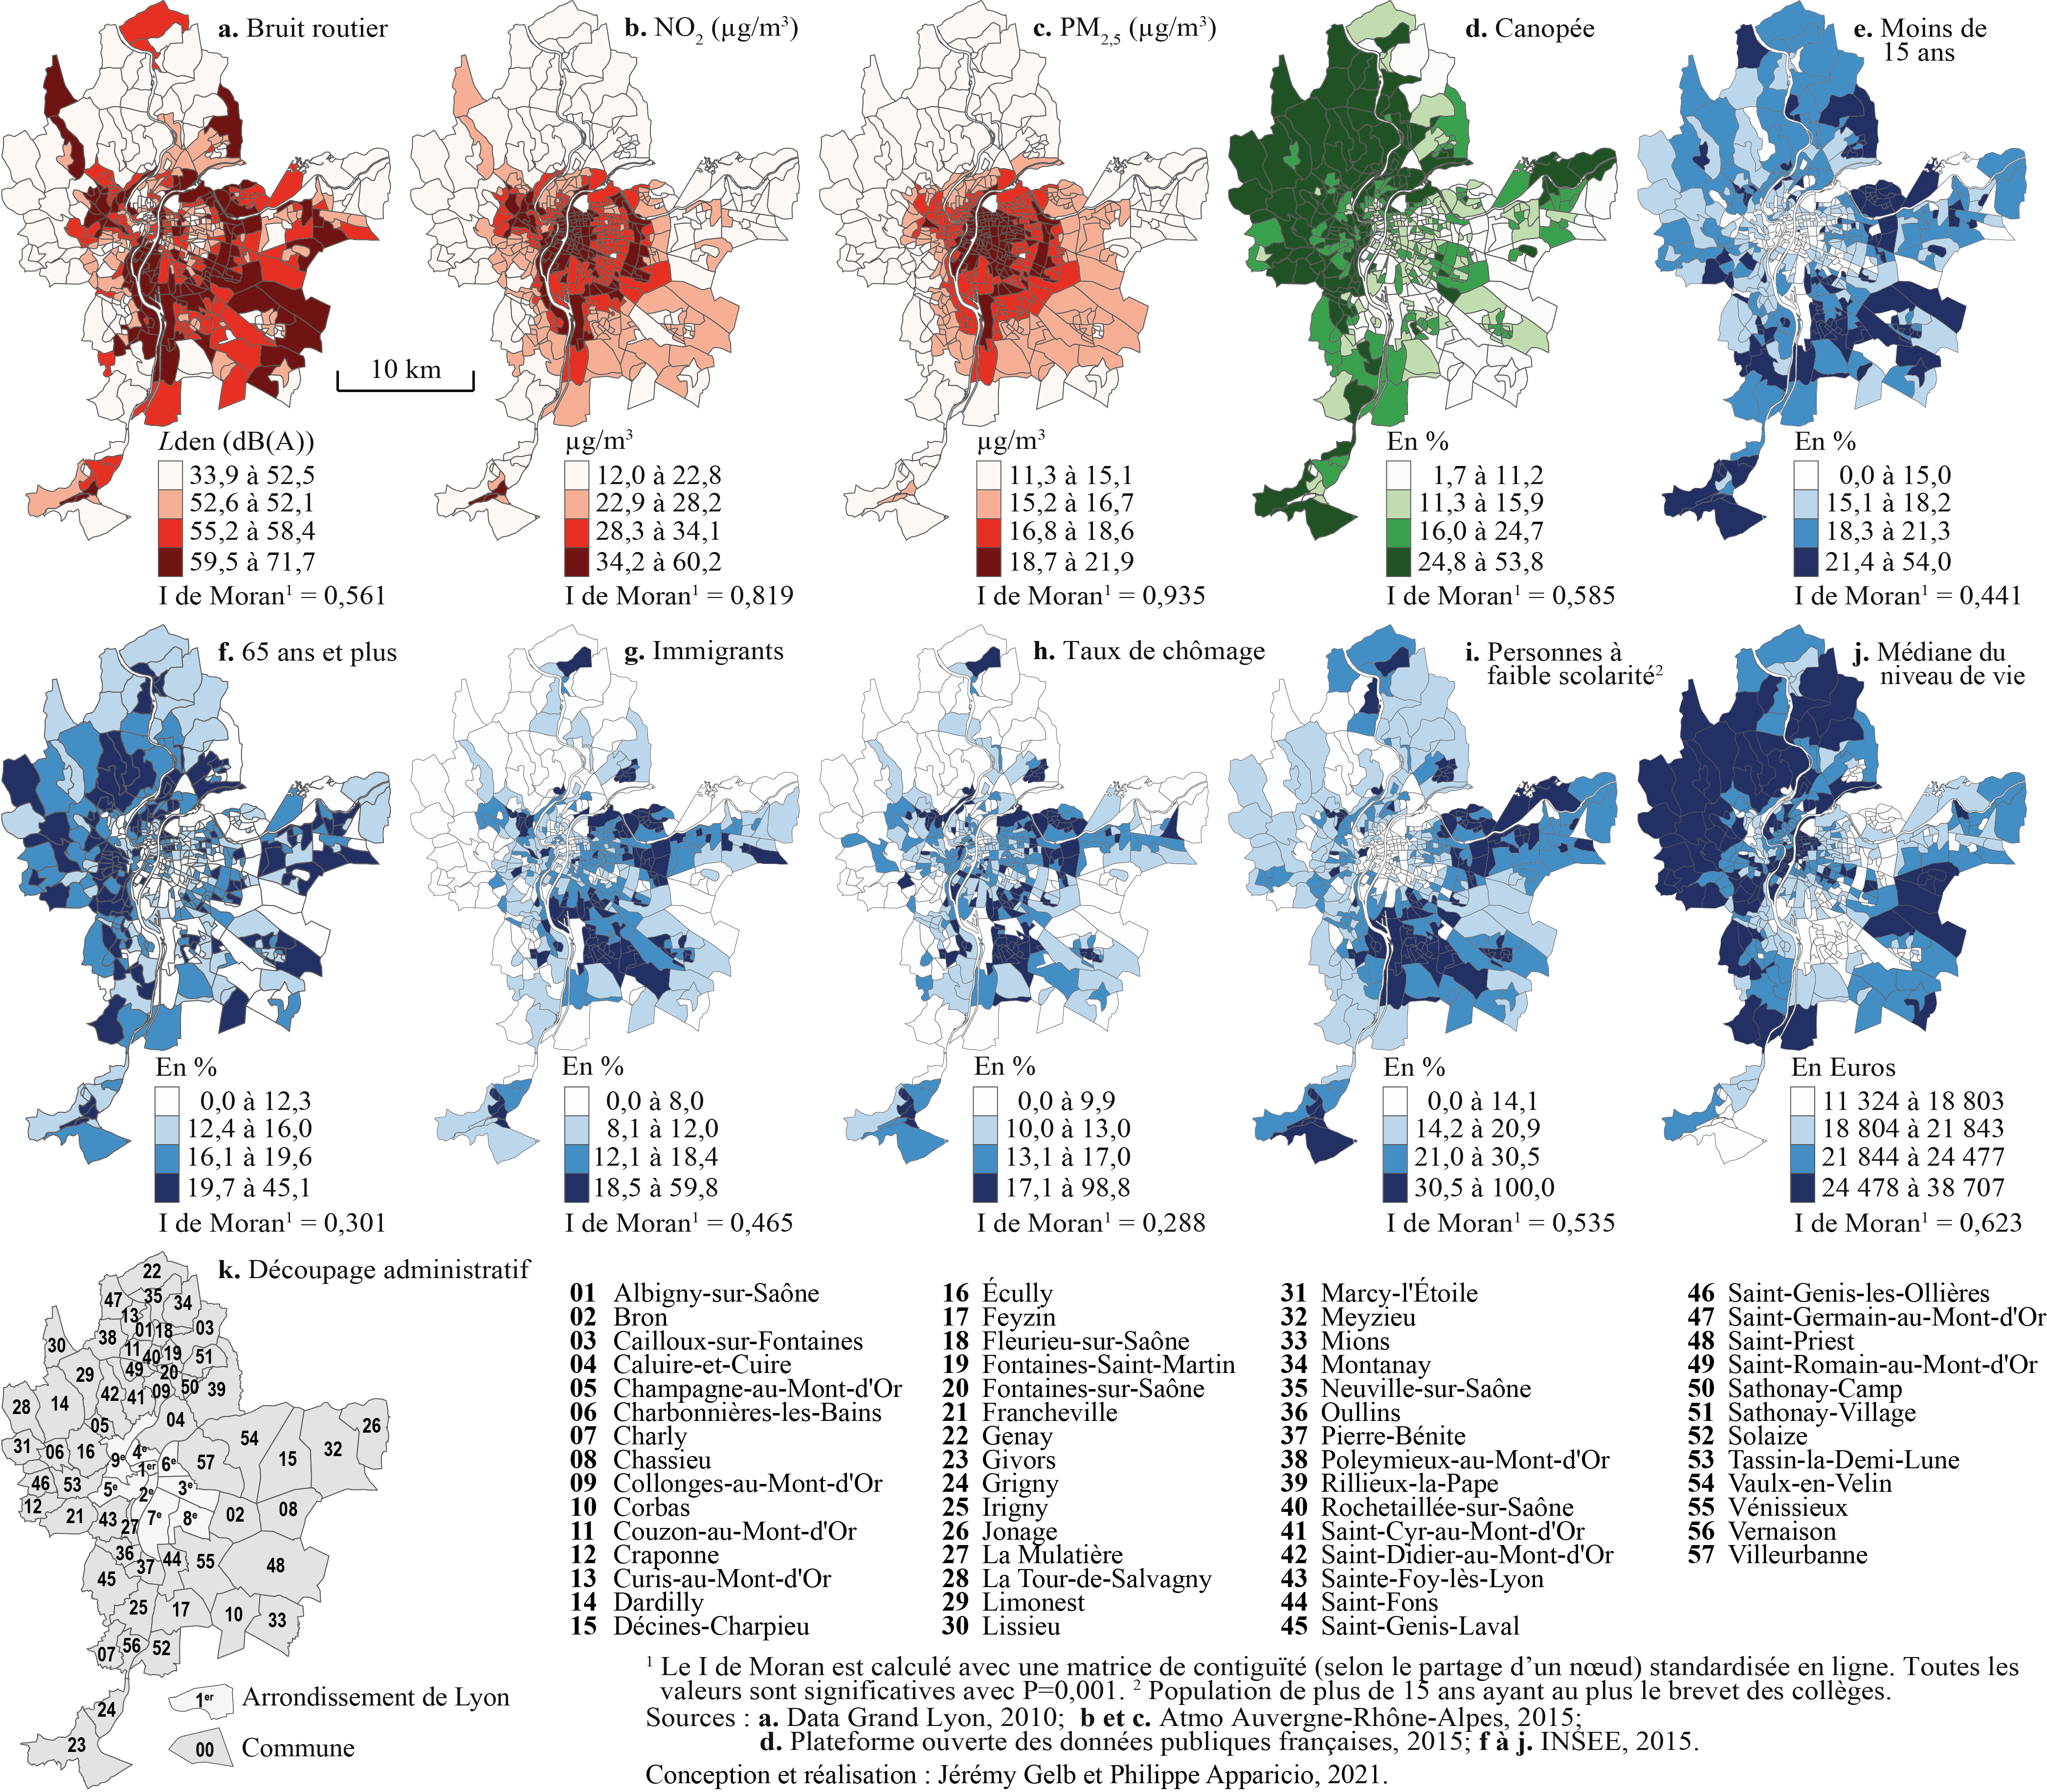
\includegraphics[width=1\linewidth]{images/analysesfactorielles/Figure3Data} 

}

\caption{Cartographie des dix variables utilisées pour l'ACP}\label{fig:datacartoacp}
\end{figure}

\begin{bloc_objectif}
\textbf{Trois étapes pour bien analyser une ACP et comprendre la signification des axes factoriels~:}

\begin{enumerate}
\def\labelenumi{\arabic{enumi}.}
\tightlist
\item
  Interprétation des résultats des valeurs propres pour identifier le nombre d'axes (de composantes principales) à retenir. L'enjeu est de garder un nombre d'axes limité qui résume le mieux le tableau initial (réduction des données).
\item
  Analyse des résultats pour les variables (coordonnées factorielles, cosinus carrés et contributions sur les axes retenus).
\item
  Analyse des résultats pour les individus (coordonnées factorielles, cosinus carrés et contributions sur les axes retenus).
\end{enumerate}

Les deux dernières étapes permettent de comprendre la signification des axes retenus et de les qualifier. Cette étape d'interprétation est essentielle en sciences sociales. En effet, nous avons vu dans l'introduction du chapitre que les méthodes factorielles permettent de résumer l'information d'un tableau en quelques nouvelles variables synthétiques, souvent considérées comme des variables latentes dans le jeu de données. Il convient alors de bien comprendre ces variables synthétiques (latentes) si nous souhaitons les utiliser dans une autre analyse subséquente (par exemple, les introduire dans une régression).

\end{bloc_objectif}

\hypertarget{sect12221}{%
\subsubsection{Résultats de l'ACP pour les valeurs propres}\label{sect12221}}

À titre de rappel, une ACP normée est réalisée sur des variables préalablement centrées réduites (équation \eqref{eq:scorezacpnormee}), ce qui signifie que pour chaque variable~:

\begin{itemize}
\tightlist
\item
  Nous soustrayons à chaque valeur la moyenne de la variable correspondante (centrage); la moyenne est donc égale à~0.
\item
  Nous divisons cette différence par l'écart-type de la variable correspondante (réduction); la variance est égale à~1.
\end{itemize}

\footnotesize

\begin{equation}  
z= \frac{x_i-\mu}{\sigma}
\label{eq:scorezacpnormee}
\end{equation}
\normalsize

Par conséquent, la variance totale (ou inertie totale) d'un tableau sur lequel est calculée une ACP normée est égale au nombre de variables qu'il comprend. Puisque nous l'appliquons ici à dix variables, la variance totale du tableau à réduire -- c'est-à-dire à résumer en \emph{K} nouvelles variables synthétiques, composantes principales, axes factoriels -- est donc égale à 10. Trois mesures reportées au tableau~\ref{tab:dataacpValeurPropres} permettent d'analyser les valeurs propres~:

\begin{itemize}
\tightlist
\item
  \(\mbox{VP}_k\), la valeur propre (\emph{eigenvalue} en anglais) de l'axe \emph{k} c'est-à-dire la quantité de variance du tableau initial résumé par l'axe.
\item
  \(\mbox{VP}_k / \mbox{P}\) avec \emph{P} étant le nombre de variables que comprend le tableau initial. Cette mesure représente ainsi le pourcentage de la variance totale du tableau résumé par l'axe \emph{k}, autrement dit, la quantité d'informations du tableau initial résumée par l'axe, la composante principale \emph{k}. Cela nous permet ainsi d'évaluer le pouvoir explicatif de l'axe.
\item
  Le pourcentage cumulé pour les axes.
\end{itemize}

\begin{table}

\caption{\label{tab:dataacpValeurPropres}Résultats de l'ACP pour les valeurs propres}
\centering
\fontsize{8}{10}\selectfont
\begin{tabular}[t]{rrrr}
\toprule
Composante & Valeur propre & Pourcentage & Pourc. cumulé\\
\midrule
1 & 3,543 & 35,425 & 35,425\\
2 & 2,760 & 27,596 & 63,021\\
3 & 1,042 & 10,422 & 73,443\\
4 & 0,751 & 7,511 & 80,954\\
5 & 0,606 & 6,059 & 87,013\\
\addlinespace
6 & 0,388 & 3,880 & 90,893\\
7 & 0,379 & 3,788 & 94,681\\
8 & 0,244 & 2,441 & 97,122\\
9 & 0,217 & 2,167 & 99,289\\
10 & 0,071 & 0,711 & 100,000\\
\bottomrule
\end{tabular}
\end{table}

Avant d'analyser en détail le tableau~\ref{tab:dataacpValeurPropres}, notez que la somme des valeurs propres de toutes les composantes de l'ACP est toujours égale au nombre de variables du tableau initial. Aussi, la quantité de variance expliquée (les valeurs propres) décroît de de la composante~1 à la composante~\emph{K}.

\textbf{Combien d'axes d'une ACP faut-il retenir?} Pour ce faire, deux approches sont possibles~:

\begin{itemize}
\tightlist
\item
  \textbf{Approche statistique} (avec le critère de Kaiser (\protect\hyperlink{ref-kaiser1960application}{1960})). Nous retenons uniquement les composantes qui présentent une valeur propre supérieure à~1. Rappelez-vous qu'en ACP normée, les variables sont préalablement centrées réduites et donc que leur variance respective est égale à~1. Par conséquent, une composante ayant une valeur propre inférieure à~1 a un pouvoir explicatif inférieur à celui d'une variable. À la lecture du tableau, nous retenons les trois premières composantes si nous appliquons ce critère.
\item
  \textbf{Approche empirique} basée sur la lecture des pourcentages et des pourcentages cumulés. Nous pourrons retenir uniquement les deux premières composantes. En effet, ces deux premiers facteurs résument près des deux tiers de la variance totale du tableau (63,02~\%). Cela démontre bien que l'ACP, comme les autres méthodes factorielles, est bien une méthode de réduction de données puisque nous résumons dix variables avec deux nouvelles variables synthétiques (axes, composantes principales). Pour faciliter le choix du nombre d'axes, il est fortement conseillé de construire des histogrammes à partir des valeurs propres, des pourcentages et des pourcentages cumulés (figure~\ref{fig:acpgraphvp}). Or, à la lecture de ces graphiques, nous constatons que la variance expliquée chute drastiquement après les deux premières composantes. Par conséquent, nous pouvons retenir uniquement les deux premiers axes.
\end{itemize}

\begin{bloc_astuce}
\textbf{Lecture du diagramme des valeurs propres}

Plus les variables incluses dans l'ACP sont corrélées entre elles, plus l'ACP sera intéressante~: plus les valeurs propres des premiers axes sont fortes et plus il y a des sauts importants dans le diagramme des valeurs propres. À l'inverse, lorsque les variables incluses dans l'ACP sont peu corrélées entre elles, il n'y aura pas de sauts importants dans l'histogramme, autrement dit, les valeurs propres sont uniformément décroissantes.

\end{bloc_astuce}

\begin{figure}

{\centering 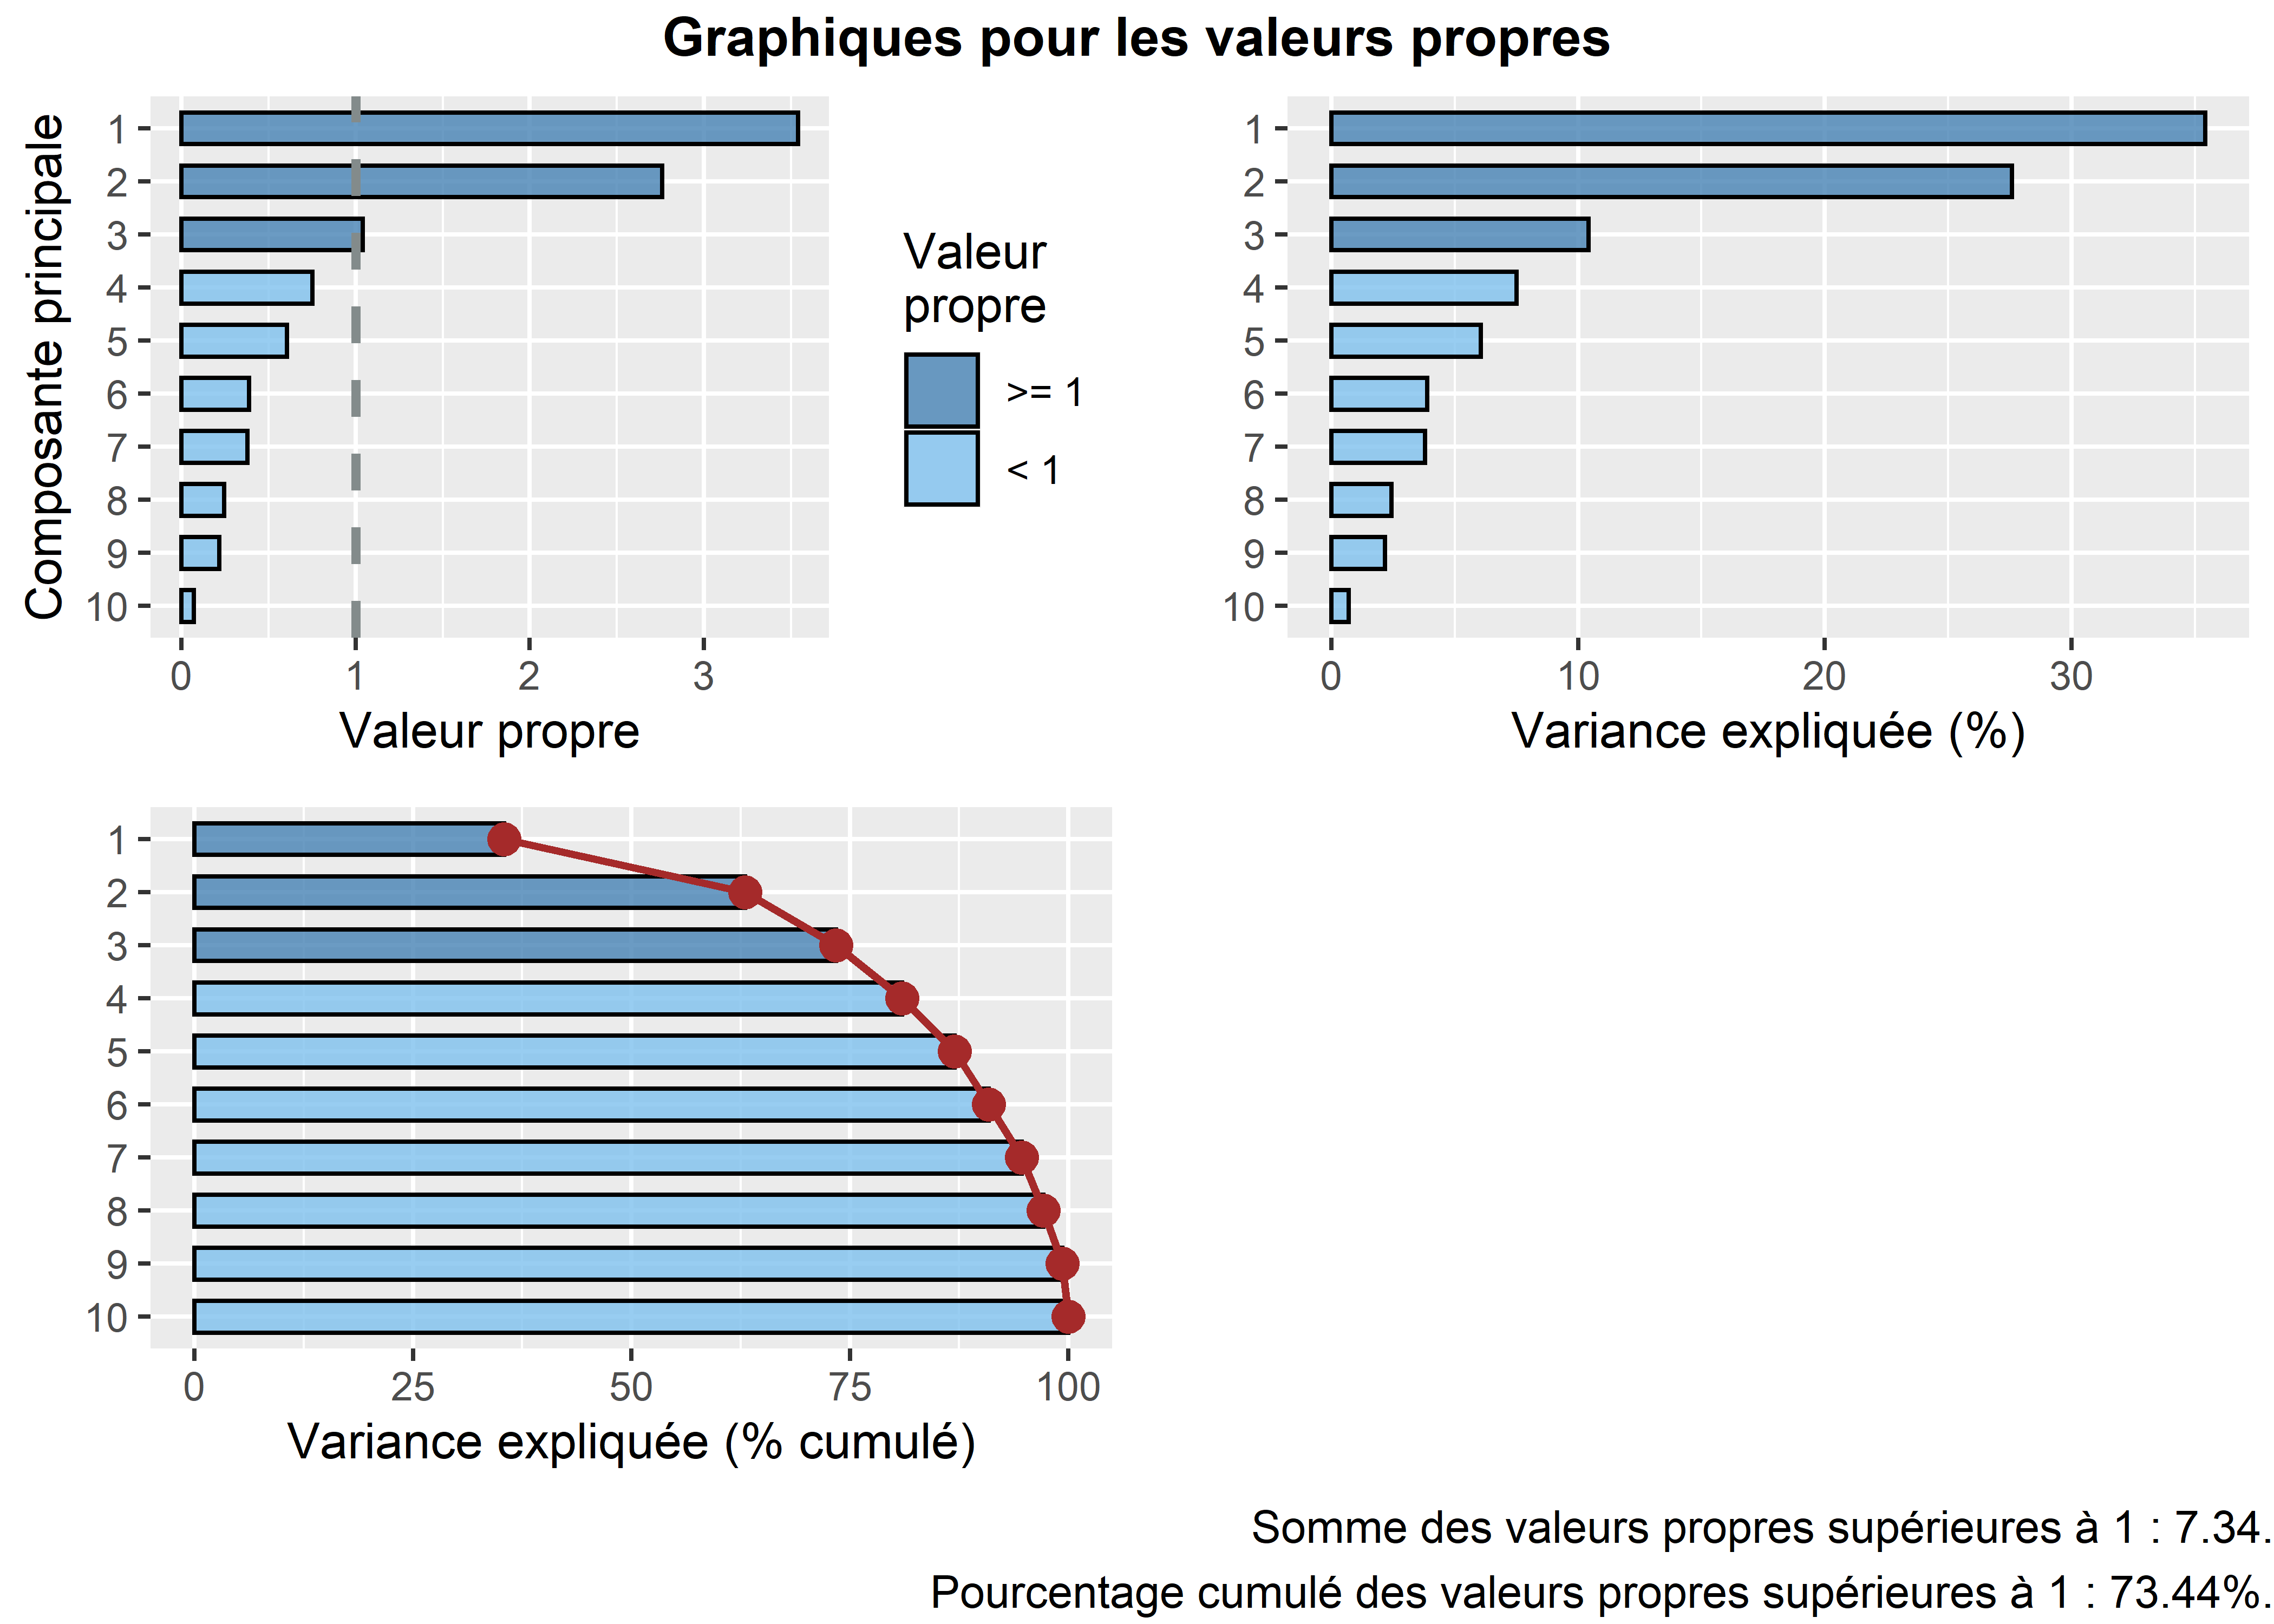
\includegraphics[width=0.75\linewidth]{livre_statistique_Phil_Jere_clean_files/figure-latex/acpgraphvp-1} 

}

\caption{Graphiques personnalisés pour les valeurs propres pour l'ACP}\label{fig:acpgraphvp}
\end{figure}

\hypertarget{sect12222}{%
\subsubsection{Résultats de l'ACP pour les variables}\label{sect12222}}

Pour qualifier les axes, quatre mesures sont disponibles pour les variables~:

\begin{itemize}
\tightlist
\item
  \textbf{Les coordonnées factorielles des variables} sont simplement les coefficients de corrélation de Pearson des variables sur l'axe \emph{k} et varient ainsi de -1 à 1 (relire au besoin la section \ref{sect043}). Pour qualifier un axe, il convient alors de repérer les variables les plus corrélées positivement et négativement sur l'axe, autrement dit, de repérer les variables situées aux extrémités l'axe.
\item
  \textbf{Les cosinus carrés des variables} (Cos\textsuperscript{2}) (appelées aussi les qualités de représentation des variables sur un axe) permettent de repérer le ou les axes qui concourent le plus à donner un sens à la variable. Elles sont en fait les coordonnées des variables mises au carré. La somme des cosinus carrés d'une variable sur tous les axes de l'ACP est donc égale à~1 (sommation en ligne).
  \textbf{La qualité de représentation d'une variable sur les \emph{n} premiers axes} est simplement la somme des cosinus carrés d'une variable sur les axes retenus. Par exemple, pour la variable \texttt{Lden}, la qualité de représentation de la variable sur le premier axe est égale~: \(\mbox{0,42}^2=\mbox{0,17}\). Pour cette même variable, la qualité de la \texttt{Lden} sur les trois premiers axes est égale à~: \(\mbox{0,17}+\mbox{0,32}+\mbox{0,26}=\mbox{0,75}\).
\item
  \textbf{Les contributions des variables} permettent de repérer celles qui participent le plus à la formation d'un axe. Elles s'obtiennent en divisant les cosinus carrés par la valeur propre de l'axe multiplié par 100. La somme des contributions des variables pour un axe donné est donc égale à 100 (sommation en colonne). Par exemple, pour la variable \texttt{Lden}, la contribution sur le premier axe est égale~: \(\mbox{0,174} / \mbox{3,543} \times \mbox{100}= \mbox{4,920 }%
  \).
\end{itemize}

Les résultats de l'ACP pour les variables sont présentés au tableau~\ref{tab:dataacpCoordVars}.

\begin{table}

\caption{\label{tab:dataacpCoordVars}Résultats de l'ACP pour les variables}
\centering
\fontsize{8}{10}\selectfont
\begin{tabular}[t]{lrrrrrrrrrr}
\toprule
\multicolumn{1}{c}{ } & \multicolumn{3}{c}{Coordonnées} & \multicolumn{4}{c}{Cosinus carrés} & \multicolumn{3}{c}{Contributions} \\
\cmidrule(l{3pt}r{3pt}){2-4} \cmidrule(l{3pt}r{3pt}){5-8} \cmidrule(l{3pt}r{3pt}){9-11}
Variable & 1 & 2 & 3 & 1 & 2 & 3 & Qualité & 1 & 2 & 3\\
\midrule
Lden & 0,42 & 0,57 & 0,51 & 0,17 & 0,32 & 0,26 & 0,75 & 4,92 & 11,64 & 24,80\\
NO2 & 0,15 & 0,93 & 0,19 & 0,02 & 0,86 & 0,04 & 0,92 & 0,66 & 31,07 & 3,54\\
PM25 & 0,19 & 0,92 & 0,03 & 0,04 & 0,84 & 0,00 & 0,87 & 1,01 & 30,36 & 0,12\\
VegHautPrt & -0,40 & -0,42 & 0,40 & 0,16 & 0,18 & 0,16 & 0,50 & 4,63 & 6,35 & 15,46\\
Pct0\_14 & 0,55 & -0,53 & 0,08 & 0,30 & 0,28 & 0,01 & 0,59 & 8,61 & 10,28 & 0,55\\
\addlinespace
Pct\_65 & -0,41 & -0,27 & 0,72 & 0,17 & 0,07 & 0,51 & 0,75 & 4,73 & 2,66 & 49,26\\
Pct\_Img & 0,87 & -0,09 & 0,11 & 0,76 & 0,01 & 0,01 & 0,78 & 21,56 & 0,29 & 1,08\\
TxChom1564 & 0,77 & -0,09 & -0,07 & 0,60 & 0,01 & 0,00 & 0,61 & 16,89 & 0,27 & 0,45\\
Pct\_brevet & 0,73 & -0,43 & 0,22 & 0,53 & 0,19 & 0,05 & 0,77 & 14,94 & 6,81 & 4,61\\
NivVieMed & -0,88 & 0,09 & 0,04 & 0,78 & 0,01 & 0,00 & 0,79 & 22,06 & 0,28 & 0,14\\
\bottomrule
\end{tabular}
\end{table}

\textbf{Analyse de la première composante principale (valeur propre de 3,54, 35,43~\%)}

\begin{itemize}
\item
  À la lecture des contributions, il est clair que quatre variables contribuent grandement à la formation de l'axe~1~: \texttt{NivVieMed} (22,06~\%),
  \texttt{Pct\_Img} (21,56~\%), \texttt{TxChom1564} (16,89~\%) et \texttt{Pct\_brevet} (14,94~\%). Il convient alors d'analyser en détail leurs coordonnées factorielles et leurs cosinus carrés.
\item
  À la lecture des coordonnées factorielles, nous constatons que trois variables socioéconomiques sont fortement corrélées positivement avec l'axe~1, soit le \emph{pourcentage d'immigrants} (0,87), le \emph{taux de chômage} (0,77) le \emph{pourcentage de personnes avec une faible scolarité} (0,73). À l'autre extrémité, la \emph{médiane du niveau de vie} (en Euros) est négativement corrélée avec l'axe~1. Comment interpréter ce résultat? Premièrement, cela signifie que plus la valeur de l'axe 1 est positive et élevée, plus celles des trois variables (\texttt{Pct\_Img},\texttt{TxChom1564} et \texttt{Pct\_brevet}) sont aussi élevées (corrélations positives) et plus la valeur de \texttt{NivVieMed} est faible (corrélation négative). Inversement, plus la valeur de l'axe~1 est négative et faible, les valeurs de \texttt{Pct\_Img}, \texttt{TxChom1564} et \texttt{Pct\_brevet} sont faibles et plus celle de \texttt{NivVieMed} est forte. Deuxièmement, cela signifie que les trois variables (\texttt{Pct\_Img},\texttt{TxChom1564} et \texttt{Pct\_brevet}) sont fortement corrélées positivement entre elles puisqu'elles se situent sur la même extrémité de l'axe et qu'elles sont toutes trois négativement corrélées avec la variable \texttt{NivVieMed}. Cela peut être rapidement confirmé avec la matrice de corrélation entre les dix variables (tableau~\ref{tab:dataacpMatriceCorr}).
\item
  À la lecture des cosinus carrés de l'axe~1, nous constatons que plus des trois quarts de la dispersion/de l'information des variables \texttt{NivVieMed} (0,78) et \texttt{Pct\_Img} (0,76) est concentrée sur l'axe~1.
\end{itemize}

\begin{table}

\caption{\label{tab:dataacpMatriceCorr}Matrice de corrélation de Pearson entre les variables utilisées pour l'ACP}
\centering
\fontsize{8}{10}\selectfont
\begin{tabular}[t]{lrrrrrrrrrr}
\toprule
Variable & A & B & C & D & E & F & G & H & I & J\\
\midrule
A. Lden &  & 0,62 & 0,49 & -0,23 & 0,04 & -0,09 & 0,28 & 0,19 & 0,14 & -0,26\\
B. NO2 & 0,62 &  & 0,90 & -0,28 & -0,34 & -0,21 & 0,07 & 0,04 & -0,25 & -0,04\\
C. PM25 & 0,49 & 0,90 &  & -0,39 & -0,34 & -0,26 & 0,12 & 0,07 & -0,25 & -0,10\\
D. VegHautPrt & -0,23 & -0,28 & -0,39 &  & 0,04 & 0,32 & -0,22 & -0,18 & -0,14 & 0,32\\
E. Pct0\_14 & 0,04 & -0,34 & -0,34 & 0,04 &  & -0,12 & 0,46 & 0,36 & 0,54 & -0,45\\
\addlinespace
F. Pct\_65 & -0,09 & -0,21 & -0,26 & 0,32 & -0,12 &  & -0,24 & -0,30 & 0,00 & 0,32\\
G. Pct\_Img & 0,28 & 0,07 & 0,12 & -0,22 & 0,46 & -0,24 &  & 0,66 & 0,64 & -0,73\\
H. TxChom1564 & 0,19 & 0,04 & 0,07 & -0,18 & 0,36 & -0,30 & 0,66 &  & 0,47 & -0,62\\
I. Pct\_brevet & 0,14 & -0,25 & -0,25 & -0,14 & 0,54 & 0,00 & 0,64 & 0,47 &  & -0,67\\
J. NivVieMed & -0,26 & -0,04 & -0,10 & 0,32 & -0,45 & 0,32 & -0,73 & -0,62 & -0,67 & \\
\bottomrule
\end{tabular}
\end{table}

\textbf{Analyse de la deuxième composante principale (valeur propre de 2,76, 27,60~\%)}

\begin{itemize}
\tightlist
\item
  À la lecture des contributions, trois variables environnementales contribuent à la formation de l'axe~1~: principalement, celles sur la pollution de l'air (\texttt{NO2}~=~31,07~\% et \texttt{PM25}~=~30,36~\%) et secondairement, sur le bruit routier (\texttt{Lden}~=~11,64~\%).
\item
  À la lecture des coordonnées factorielles, ces trois variables sont fortement corrélées positivement avec l'axe 2~: \texttt{NO2} (0,93), \texttt{PM25} (0,92) et \texttt{Lden} (0,57). À l'autre extrémité de l'axe, la variable \texttt{Pct0\_14} est négativement, mais pas fortement corrélée négativement (-0,53). La lecture de la matrice de corrélation au tableau~\ref{tab:dataacpMatriceCorr} confirme que ces trois variables environnementales sont fortement corrélées positivement entre elles (par exemple, un coefficient de corrélation de Pearson de 0,90 entre \texttt{NO2} et \texttt{PM25}).
\item
  À la lecture des cosinus carrés de l'axe~2, nous constatons que près de 90~\% de la dispersion/de l'information des variables \texttt{NO2} (0,86) et \texttt{PM25} (0,84) est concentré sur l'axe~1.
\end{itemize}

\textbf{Analyse de la troisième composante principale (valeur propre de 1,042, 10,42~\%)}

\begin{itemize}
\tightlist
\item
  Le \emph{pourcentage de personnes âgées} (\texttt{Pct\_65}) contribue principalement à la formation de l'axe avec lequel est corrélée positivement (contribution de 49,26~\% et coordonnée factorielle de 0,72). S'en suit, la variable \texttt{Lden} qui joue un rôle beaucoup moins important (contribution de 24,80~\% et coordonnée factorielle de 0,51).
\end{itemize}

\begin{bloc_astuce}
\textbf{Lien entre la valeur propre d'un axe et le nombre de variables contribuant à sa formation}

Vous auvez compris que plus la valeur propre d'un axe est forte, plus il y a potentiellement de variables qui concourent à sa formation. Cela explique que pour la troisième composante qui a une faible valeur propre (1,042), seule une variable contribue significativement à sa formation.

\end{bloc_astuce}

\textbf{Analyse de la qualité de représentation des variables sur les premiers axes de l'ACP}

À titre de rappel, la qualité est simplement la somme des cosinus carrés d'une variable sur les axes retenus. Si nous retenons trois axes, les six variables qui sont le mieux résumées --~et qui ont donc le plus d'influence sur les résultats de l'ACP~-- sont ~:\texttt{NO2} (0,92), \texttt{PM25} (0,87), \texttt{NivVieMed} (0,79), \texttt{Pct\_Img} (0,78), \texttt{Pct\_brevet} (0,77) et\texttt{Lden} (0,75).

\textbf{Qualification, dénomination d'axes factoriels}

L'analyse des coordonnées, contributions et cosinus carrés doit vous permettre de formuler un intitulé pour chacun des axes retenus. Nous pouvons ainsi proposer les intitulés suivants~:

\begin{itemize}
\tightlist
\item
  \emph{Niveau de défavorisation socioéconomique} (axe~1). Plus la valeur de l'axe est élevé, plus le niveau de défavorisation de l'entité spatiale (IRIS) est élevé.
\item
  \emph{Qualité environnementale} (axe~2). Plus la valeur de l'axe est forte, plus les niveaux de pollution atmosphérique (dioxyde d'azote et particules fines) et de bruit (Lden) sont élevés.
\end{itemize}

\textbf{Le recours à des graphiques pour analyser les résultats de l'ACP pour des variables}

Plus le nombre de variables utilisées pour calculer l'ACP est important, plus l'analyse des coordonnées factorielles, des cosinus carrés et des contributions reportés dans un tableau devient fastidieuse. Puisque l'ACP a été calculée sur uniquement dix variables, l'analyse des valeurs du tableau~\ref{tab:dataacpCoordVars} a donc été assez facile et rapide. Imaginez maintenant que nous réalisons une ACP sur une centaine de variables, la taille du tableau des résultats pour les variables sera considérable\ldots{} Par conséquent, il est recommandé de construire plusieurs graphiques qui facilitent l'analyse des résultats pour les variables.

Par exemple, à la figure~\ref{fig:acpgraphvarscoords}, nous avons construit des graphiques avec les coordonnées factorielles sur les trois premiers axes de l'ACP. En un coup d'œil, il est facile de repérer les variables plus corrélées positivement ou négativement avec chacun d'entre eux.
Aussi, il est fréquent de construire un nuage de points avec les coordonnées des variables sur les deux premiers axes factoriels, soit un graphique communément appelé \textbf{nuage de points des variables sur le premier plan factoriel} sur lequel est représenté le cercle des corrélations (figure~\ref{fig:acp1erplanfactVars}). Bien entendu, cet exercice peut être fait avec d'autres axes factoriels (les axes 3 et 4 par exemple).

\begin{figure}

{\centering 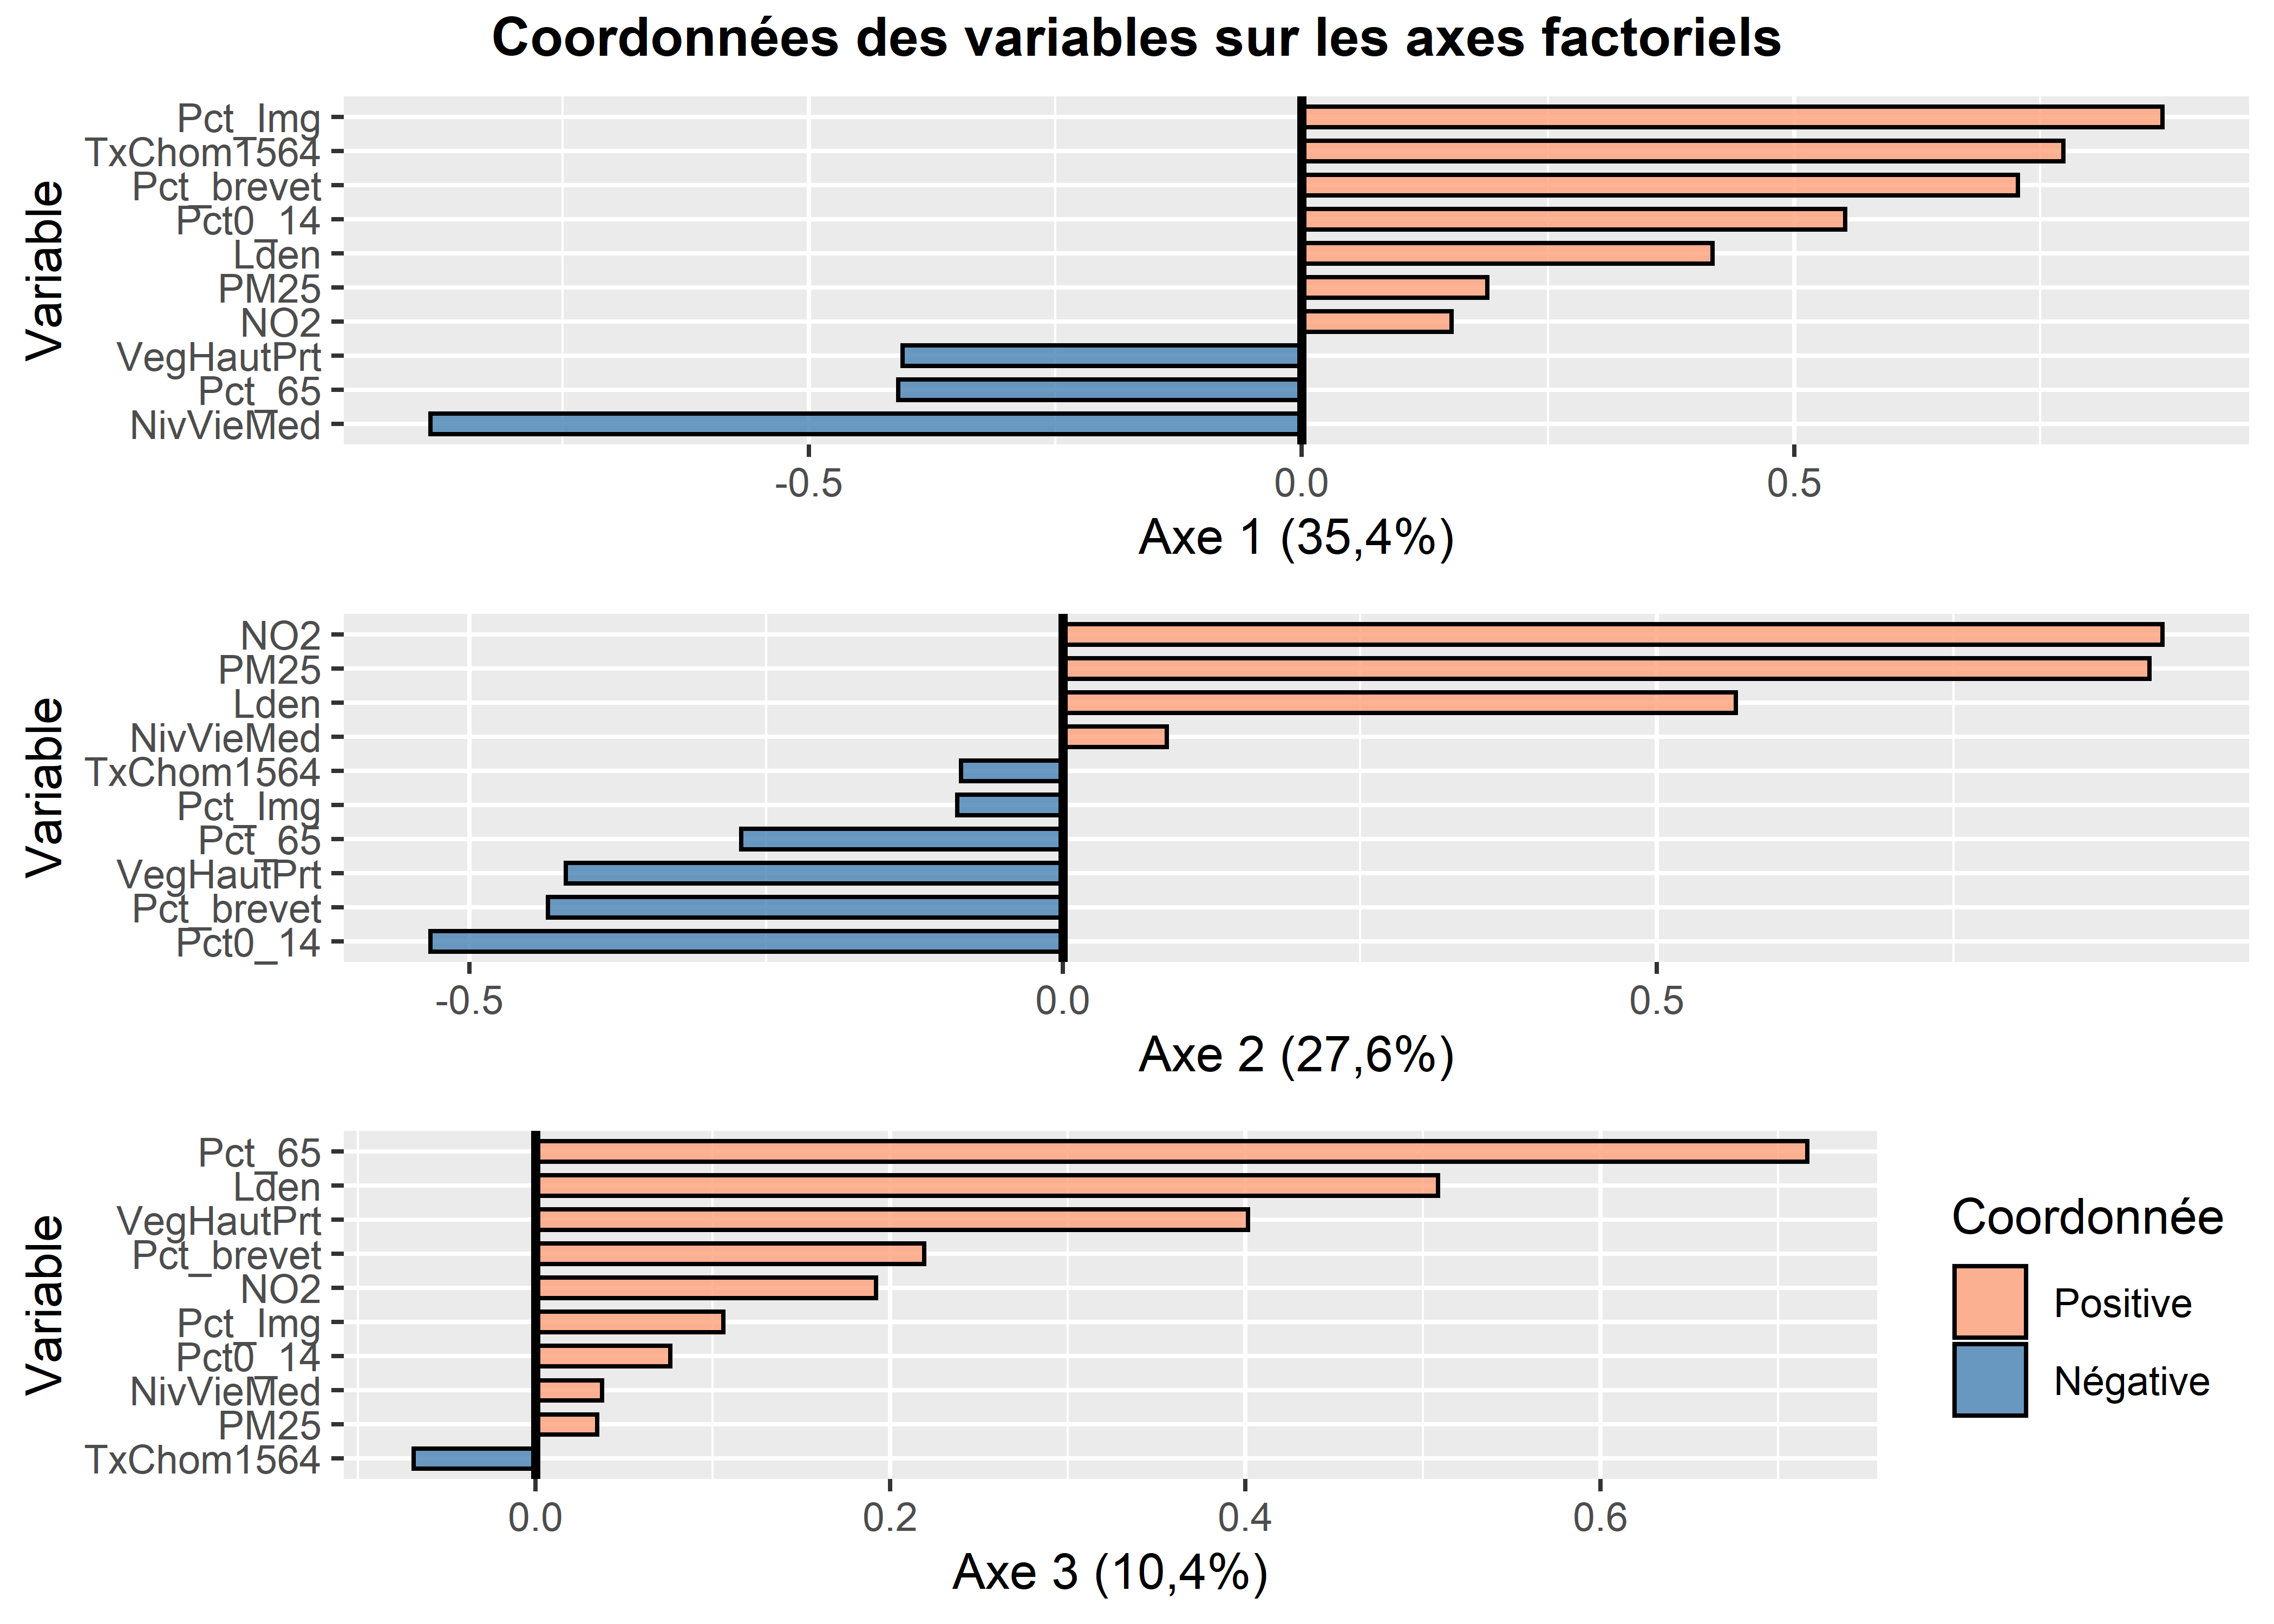
\includegraphics[width=1\linewidth]{livre_statistique_Phil_Jere_clean_files/figure-latex/acpgraphvarscoords-1} 

}

\caption{Coordonnées factorielles des variables}\label{fig:acpgraphvarscoords}
\end{figure}

\begin{figure}

{\centering 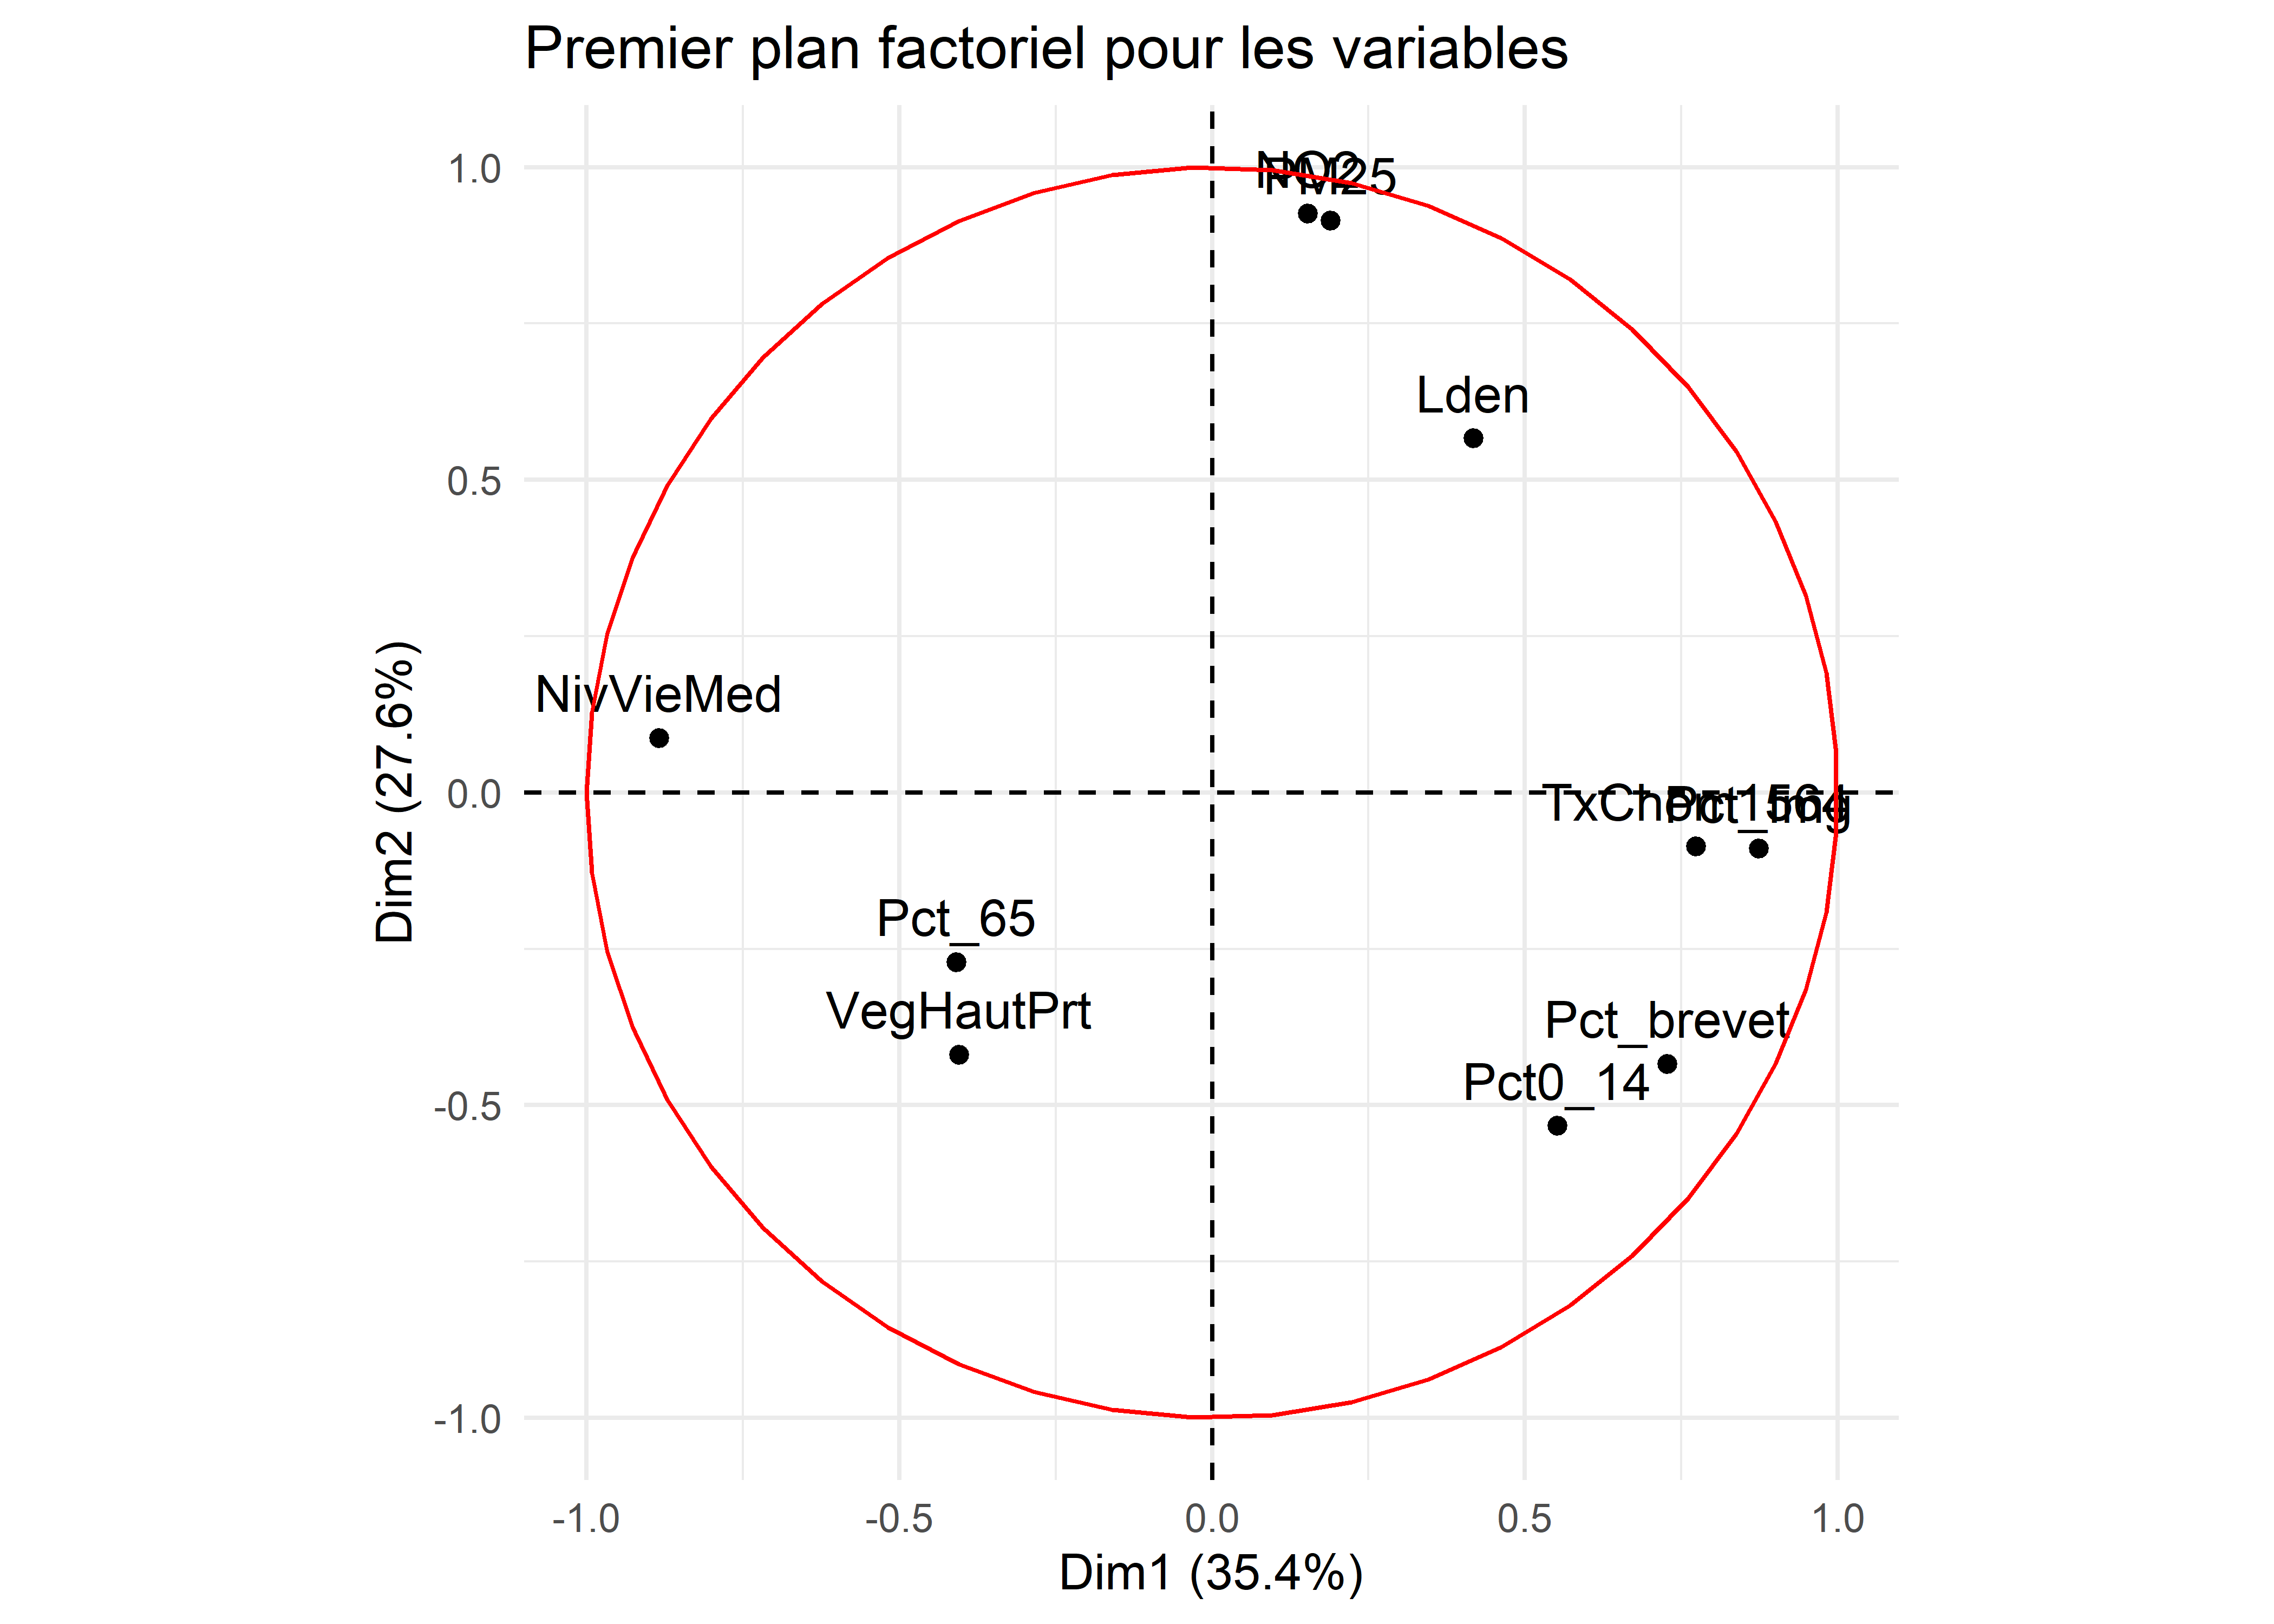
\includegraphics[width=0.75\linewidth]{livre_statistique_Phil_Jere_clean_files/figure-latex/acp1erplanfactVars-1} 

}

\caption{Premier plan factoriel de l'ACP pour les variables}\label{fig:acp1erplanfactVars}
\end{figure}

\hypertarget{sect12223}{%
\subsubsection{Résultats de l'ACP pour les individus}\label{sect12223}}

Comme pour les variables, nous retrouvons les mêmes mesures pour les individus~: les coordonnées factorielles, les cosinus carrés et les contributions. Les coordonnées factorielles des individus sont les projections orthogonales des observations sur l'axe. Puisqu'en ACP normée, les variables utilisées pour l'ACP sont centrées réduites, la moyenne des coordonnées factorielles des individus pour un axe est toujours égale à zéro. En revanche, contrairement aux coordonnées factorielles pour les variables, les coordonnées pour les individus ne varient pas de -1 à 1! Les cosinus carrés quantifient à quel point chaque axe représente chaque individu. Enfin, les contributions quantifient la contribution de chaque individu à la formation d'un axe.

Si le jeu de données comprend peu d'observations, il est toujours possible de créer un \textbf{nuage de points des individus sur le premier plan factoriel} sur lequel vous pouvez ajouter les étiquettes permettant d'identifier les observations (figure~\ref{fig:acp1erplanfactIndiv}). Ce graphique est rapidement illisible lorsque le nombre d'observations est important. Il peut rester utile si certaines des observations du jeu de données doivent faire l'objet d'une analyse spécifique.

\begin{figure}

{\centering 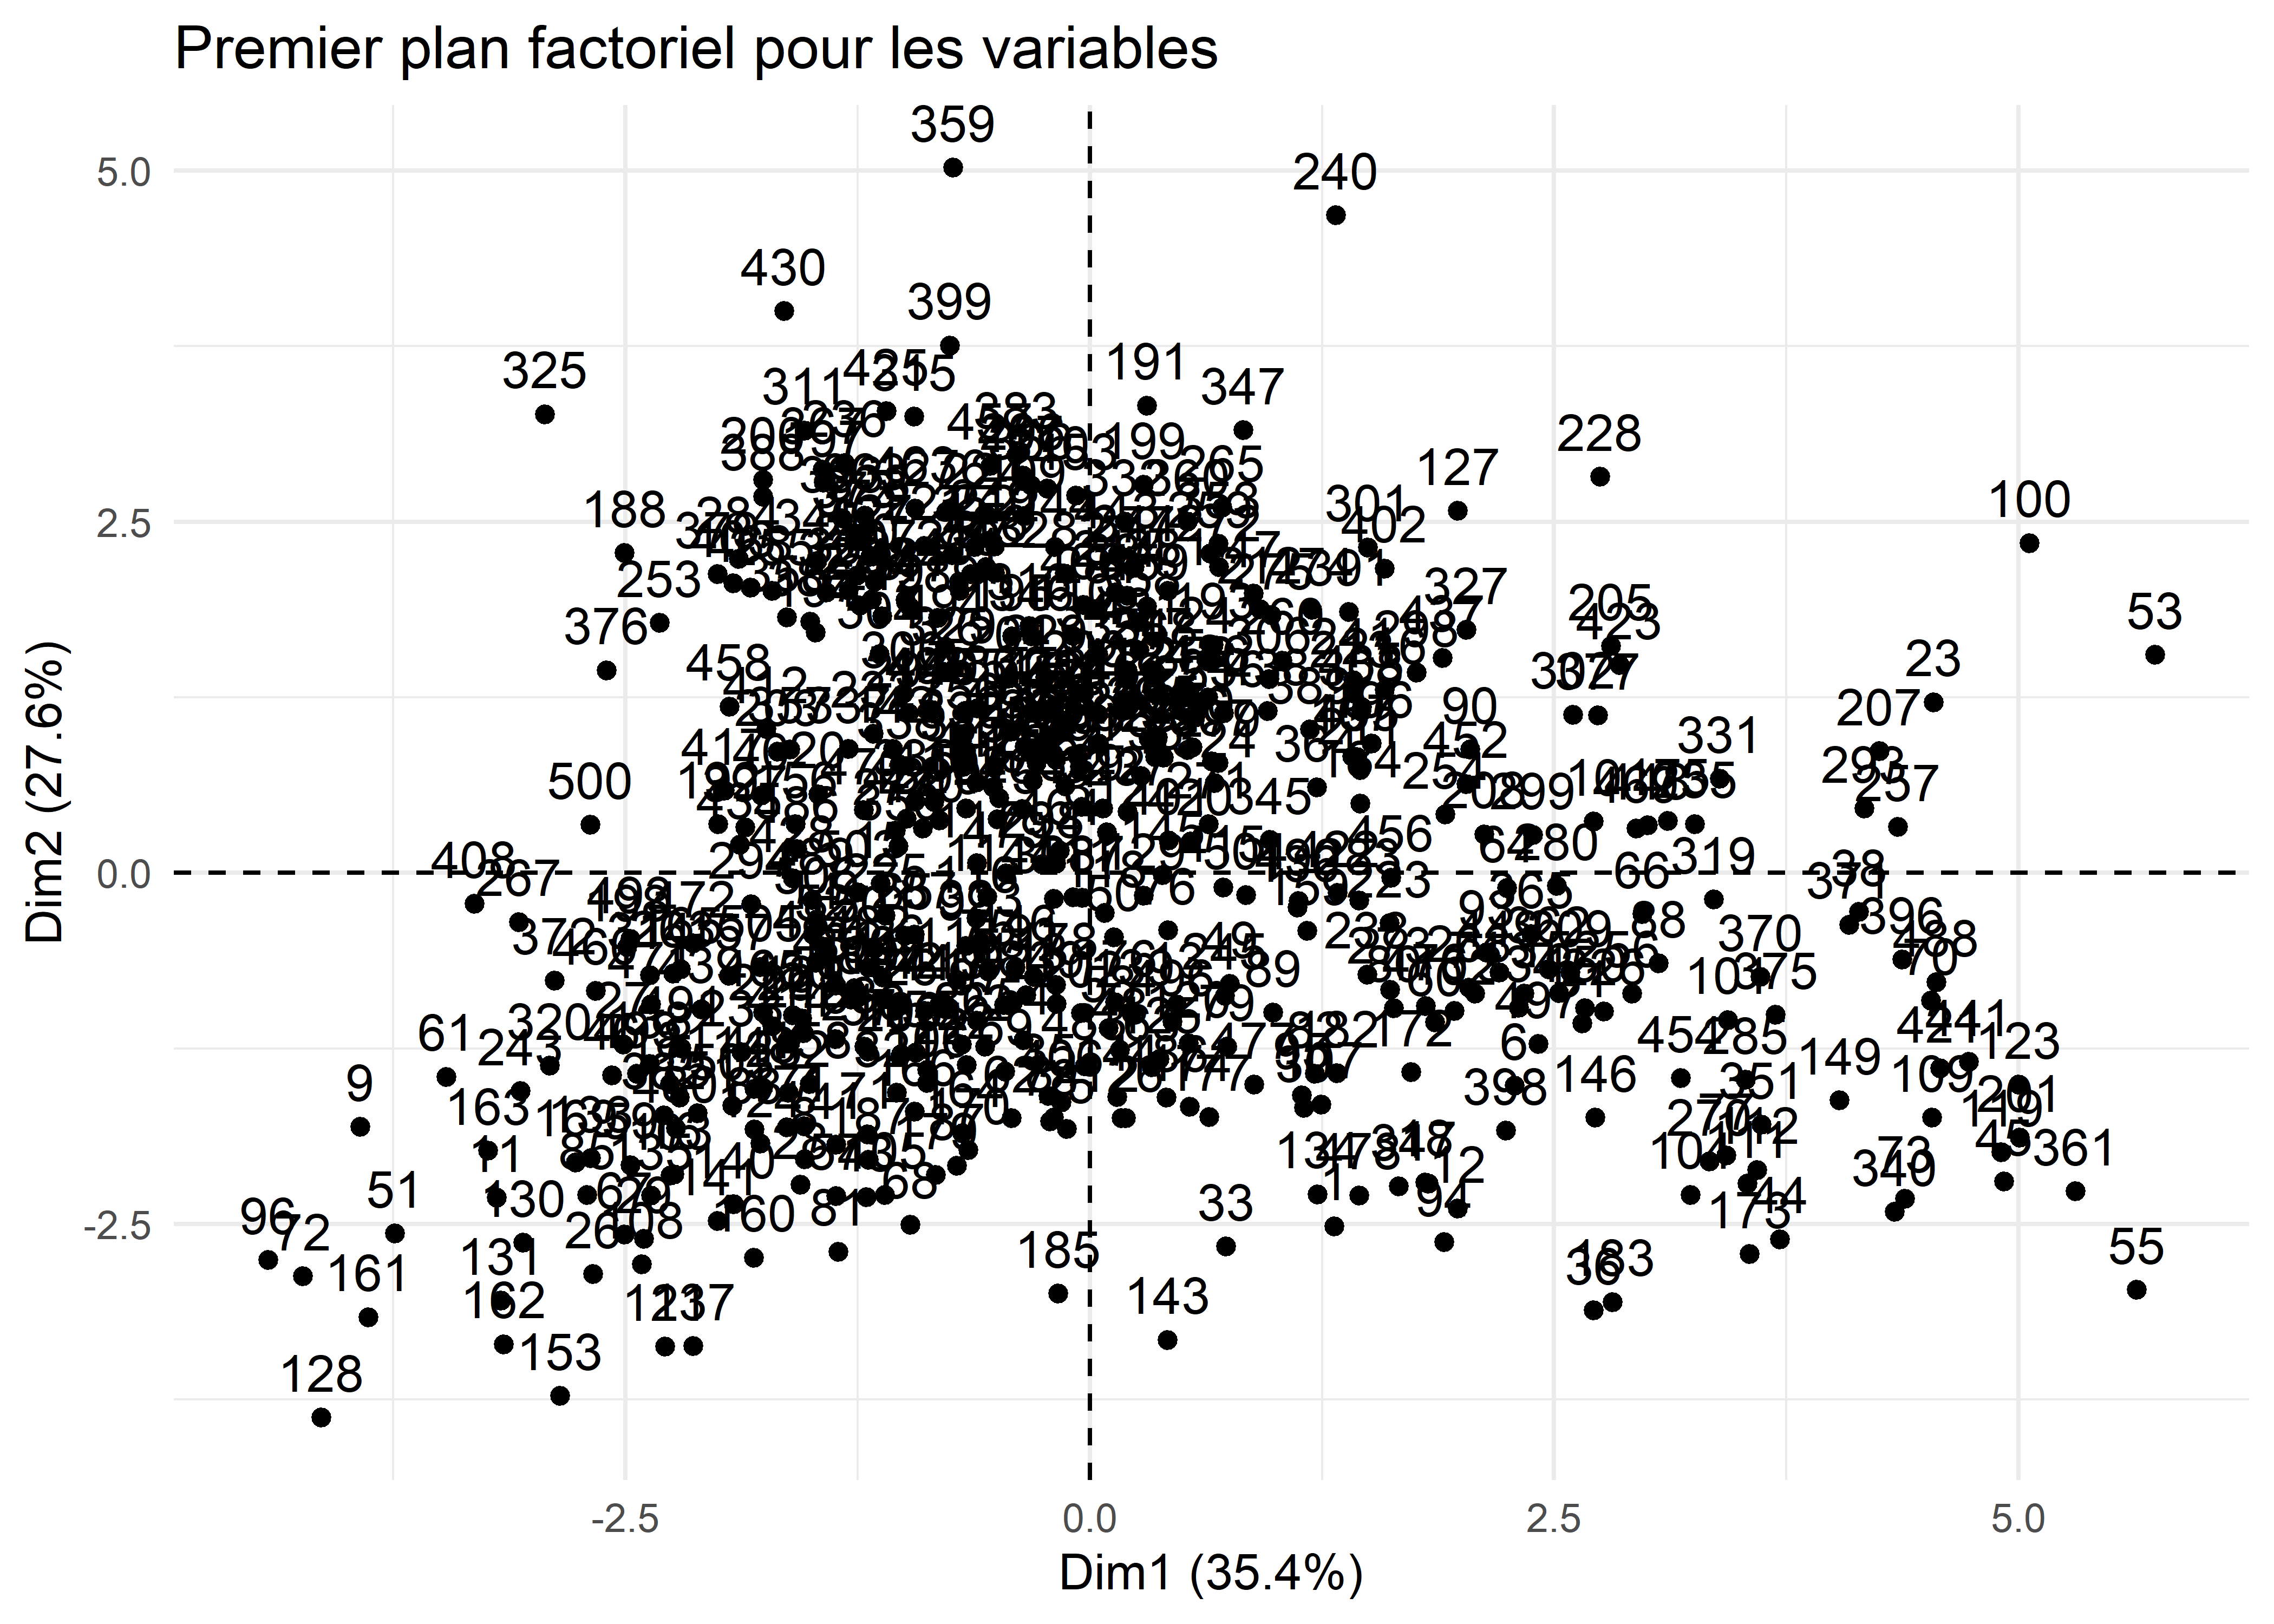
\includegraphics[width=0.75\linewidth]{livre_statistique_Phil_Jere_clean_files/figure-latex/acp1erplanfactIndiv-1} 

}

\caption{Premier plan factoriel pour les individus}\label{fig:acp1erplanfactIndiv}
\end{figure}

Lorsque les observations sont des unités spatiales, il est très intéressant de cartographier les coordonnées factorielles des individus (figure~\ref{fig:acp1erplanfactIndiv}). À la lecture de la carte choroplèthe de gauche (axe 1), nous pouvons constater que le niveau de défavorisation socioéconomique est élevé dans l'est (IRIS en vert), et inversement, très faible à l'ouest de l'agglomération (IRIS en rouge). À la lecture de la carte de droite (axe 2), sans surprise, la partie centrale de l'agglomération est caractérisée par des niveaux de pollution atmosphérique et de bruit routier bien plus élevés qu'en périphérie.

\begin{figure}

{\centering 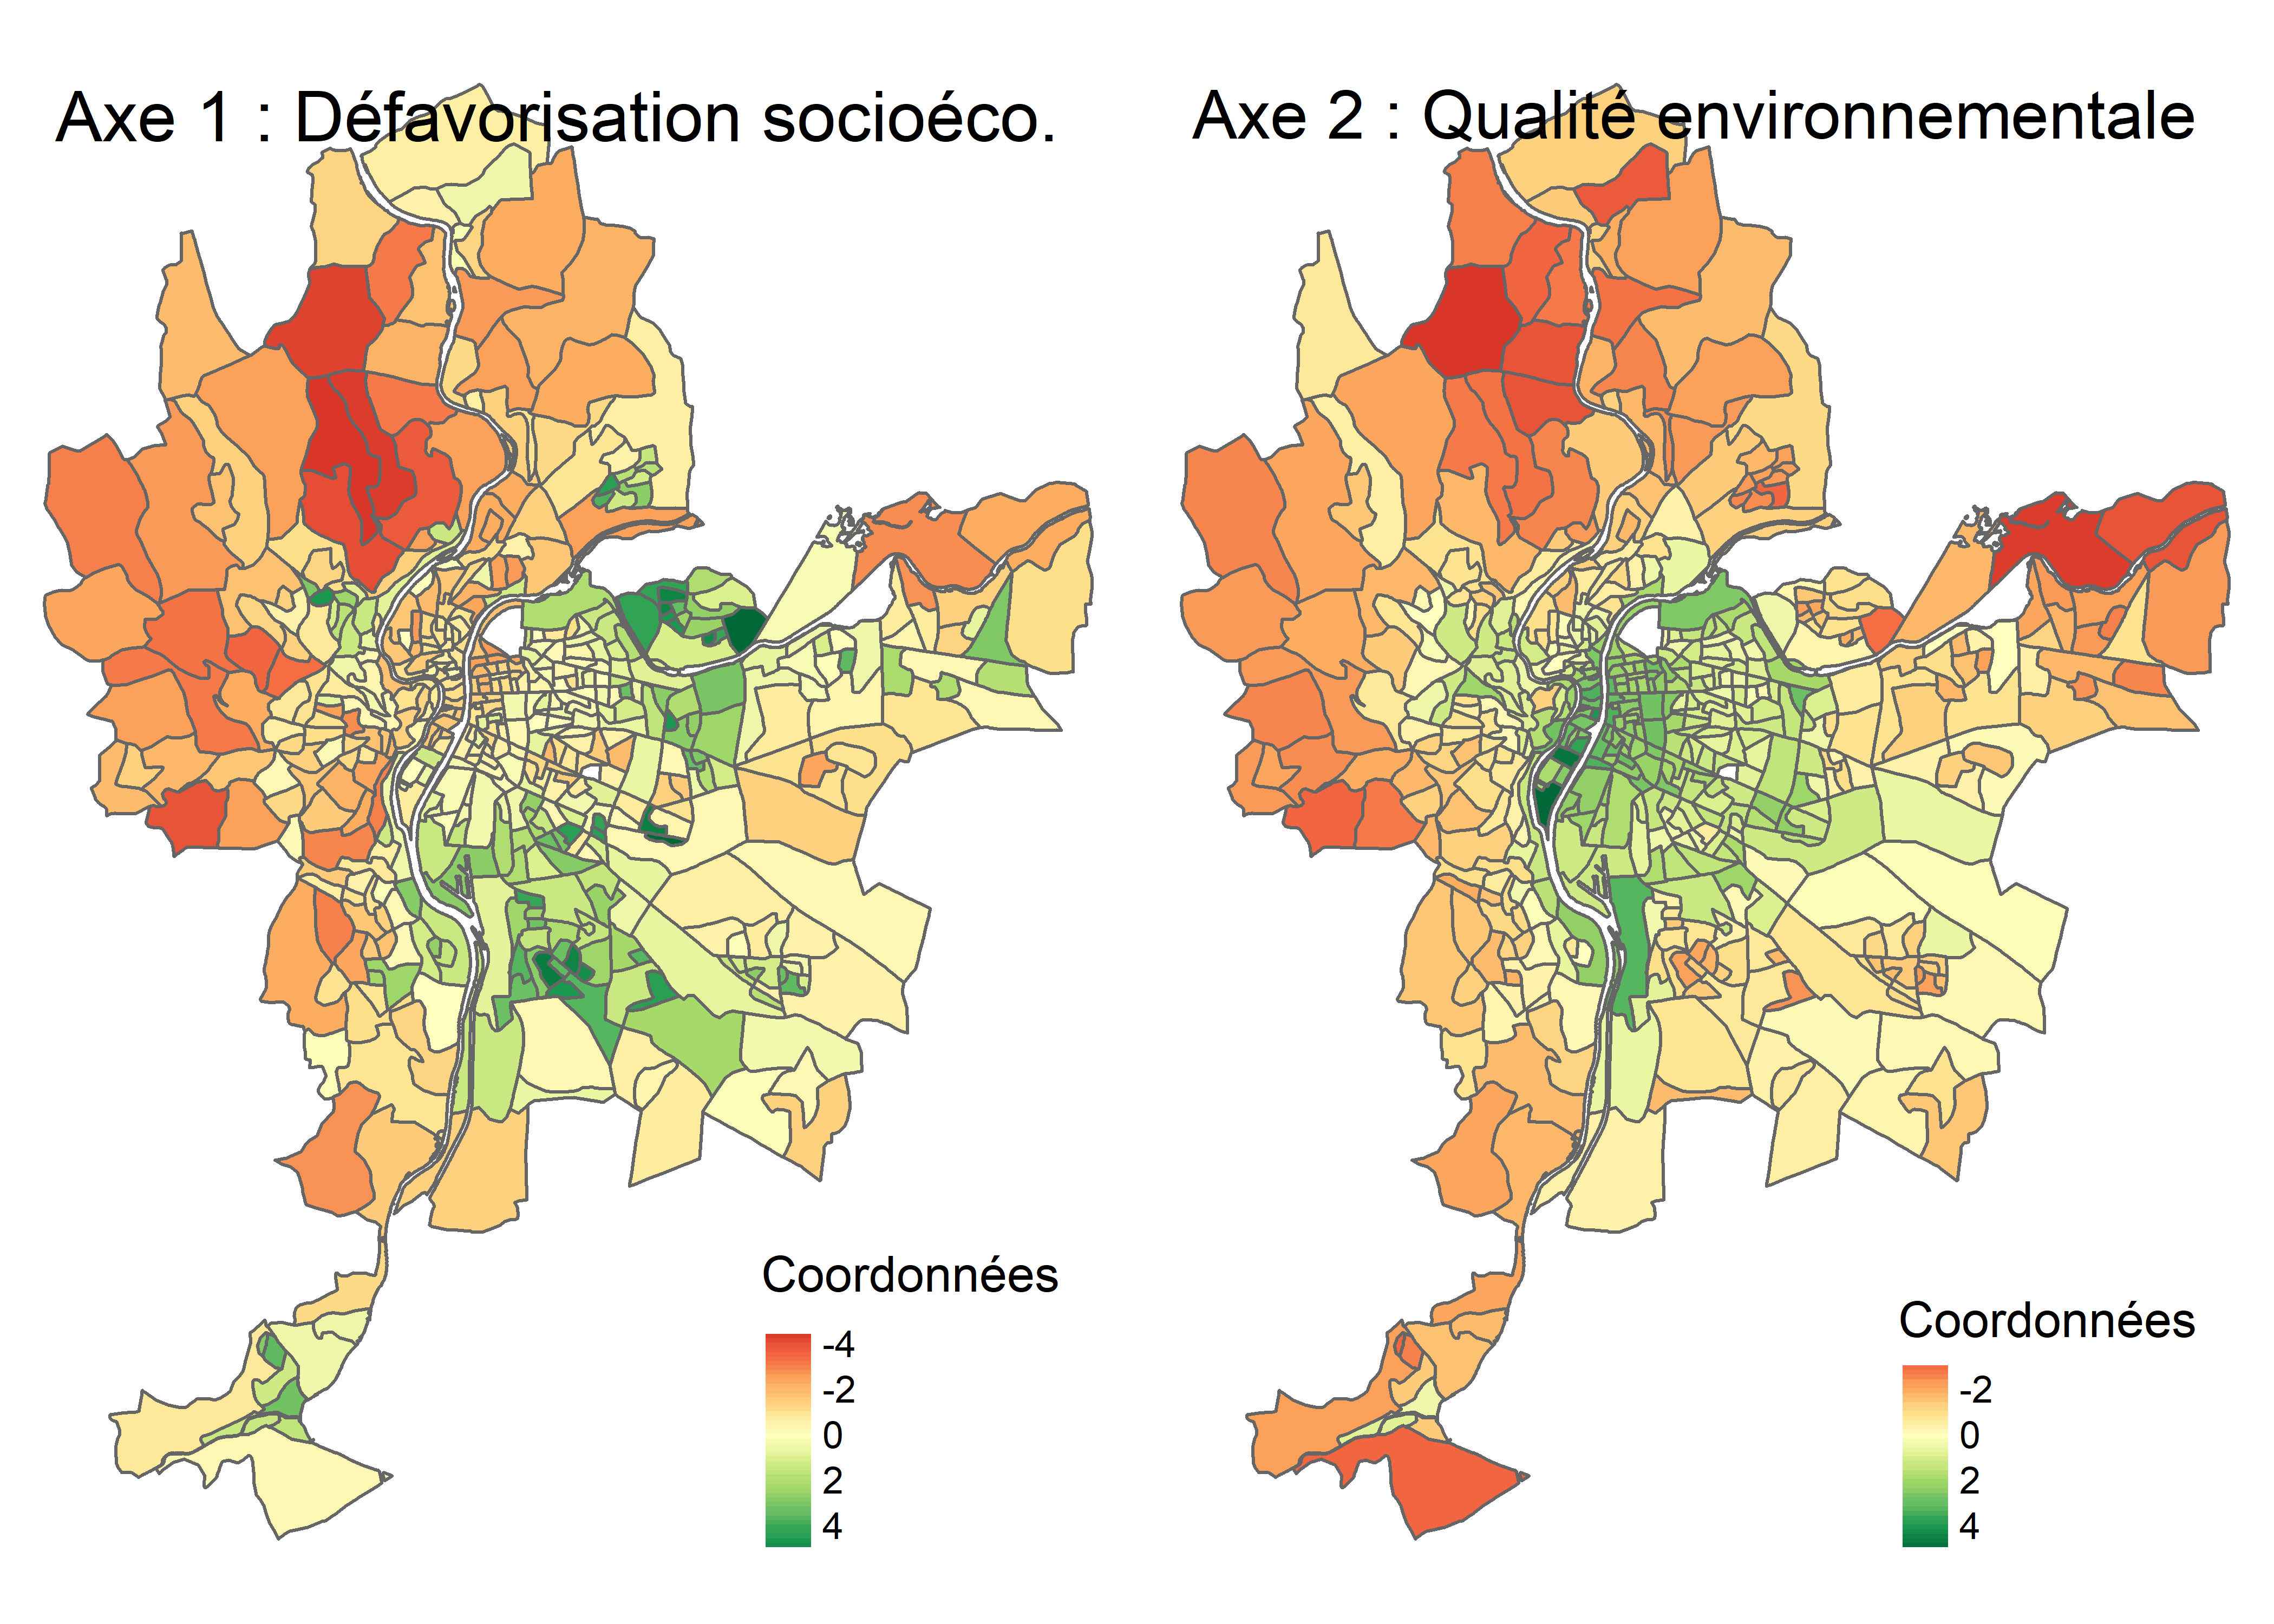
\includegraphics[width=1\linewidth]{livre_statistique_Phil_Jere_clean_files/figure-latex/acpcartoindiv-1} 

}

\caption{Cartographie des coordonnées factorielles des individus}\label{fig:acpcartoindiv}
\end{figure}

\begin{bloc_aller_loin}
Nous n'avons pas abordé plusieurs autres éléments intéressants de l'ACP.

\textbf{Ajout de variables ou d'individus supplémentaires}.

Premièrement, il est possible d'ajouter des variables continues ou des individus supplémentaires qui n'ont pas été pris en compte dans le calcul de l'ACP (figure~\ref{fig:acpvarindcorrsuppl}). Concernant les variables continues supplémentaires, il s'agit simplement de calculer leurs corrélations avec les axes retenus de l'ACP. Concernant les individus, il s'agit de les projeter sur les axes factoriels. Pour plus d'informations sur le sujet, consultez les excellents ouvrages de Ludovic Lebart, Alain Morineau et Marie Piron (\protect\hyperlink{ref-lebart1995statistique}{1995}, pp.~42-45) ou encore Jérôme Pagès (\protect\hyperlink{ref-pages2013analyse}{2013}, pp.~22-24).

\begin{figure}[H]

{\centering 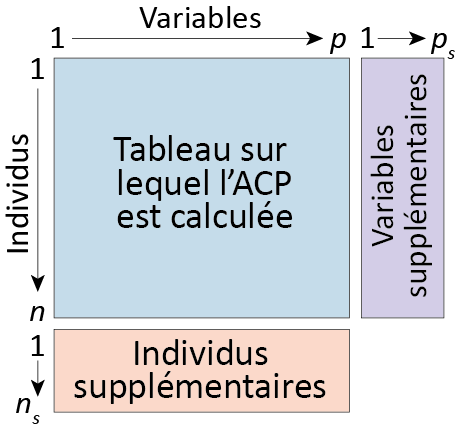
\includegraphics[width=0.28\linewidth,]{images/analysesfactorielles/AcpIndVarSuppl} 

}

\caption{Variables et individus supplémentaires pour l'ACP}\label{fig:acpvarindcorrsuppl}
\end{figure}

\textbf{Pondération des individus et des variables}.

Deuxièmement, il est possible de pondérer à la fois les individus et plus rarement les variables lors du calcul du l'ACP.

\textbf{Analyse en composantes principales non paramétrique}

Troisièmement, il est possible de calculer une ACP sur des variables préalablement transformées en rangs (section \ref{sect02552}). Cela peut être justifié lorsque les variables sont très anormalement distribuées en raison de valeurs extrêmes. Les coordonnées factorielles pour les variables sont alors le coefficient de Spearman (section \ref{sect0433}) et non de Pearson. Aussi, les variables sont centrées non pas sur leurs moyennes respectives, mais sur leurs médianes. Pour plus d'informations sur cette approche, consultez de nouveau Lebart et al.~(\protect\hyperlink{ref-lebart1995statistique}{1995}, pp.~51-52).

\textbf{Analyse en composantes principales robuste}

D'autres méthodes plus avancées qu'une ACP non paramétrique peuvent être utilisées afin d'obtenir des composantes principales qui ne sont pas influencées par des valeurs extrêmes~: les ACP robustes (Rivest et Plante \protect\hyperlink{ref-rivest1988analyse}{1988}; Hubert, Rousseeuw et Vanden Branden \protect\hyperlink{ref-hubert2005robpca}{2005}) qui peuvent être mises en œuvre, entre autres, avec le \emph{package} \texttt{roscpca}.

\end{bloc_aller_loin}

\hypertarget{sect1223}{%
\subsection{Mise en œuvre dans R}\label{sect1223}}

Plusieurs \emph{packages} permettent de calculer une ACP dans R, notamment \texttt{psych} (fonction \texttt{principal}), \texttt{ade4} (fonction \texttt{dudi.pca}) et \texttt{FactoMineR} (fonction \texttt{PCA}). Ce dernier est certainement le plus abouti. De plus, il permet également de calculer une analyse des correspondances (AFC), une analyse des correspondances multiples (ACM) et une analyse factorielle de données mixtes (AFDM). Nous utilisons donc \texttt{FactoMineR} pour mettre en œuvre les trois types de méthodes factorielles abordées dans ce chapitre (ACP, AFC et ACM). Pour l'ACP, nous exploitons un jeu de données issu du \emph{package} \texttt{geocmeans} qu'il faut préalablement charger à l'aide des lignes de code suivantes.

\begin{Shaded}
\begin{Highlighting}[]
\KeywordTok{library}\NormalTok{(geocmeans)}
\KeywordTok{data}\NormalTok{(LyonIris)}
\NormalTok{Data <-}\StringTok{ }\NormalTok{LyonIris}\OperatorTok{@}\NormalTok{data[}\KeywordTok{c}\NormalTok{(}\StringTok{"CODE_IRIS"}\NormalTok{,}\StringTok{"Lden"}\NormalTok{,}\StringTok{"NO2"}\NormalTok{,}\StringTok{"PM25"}\NormalTok{,}\StringTok{"VegHautPrt"}\NormalTok{,}
                        \StringTok{"Pct0_14"}\NormalTok{,}\StringTok{"Pct_65"}\NormalTok{,}\StringTok{"Pct_Img"}\NormalTok{,}
                        \StringTok{"TxChom1564"}\NormalTok{,}\StringTok{"Pct_brevet"}\NormalTok{,}\StringTok{"NivVieMed"}\NormalTok{)]}
\end{Highlighting}
\end{Shaded}

\hypertarget{sect12231}{%
\subsubsection{\texorpdfstring{Calcul et exploration d'une ACP avec \texttt{FactoMineR}}{Calcul et exploration d'une ACP avec FactoMineR}}\label{sect12231}}

Pour calculer l'ACP, il suffit d'utiliser la fonction \texttt{PCA} de \texttt{FactoMineR}, puis la fonction \texttt{summary(MonACP)} qui renvoie les résultats de l'ACP pour~:

\begin{itemize}
\tightlist
\item
  Les valeurs propres (section \texttt{Eigenvalues}) pour les composantes principales (\texttt{Dim.1} à \texttt{Dim.n}) avec leur variance expliquée brute (\texttt{Variance}), en pourcentage (\texttt{\%\ of\ var.}) et en pourcentage cumulé (\texttt{Cumulative\ \%\ of\ var.}).
\item
  Les dix premières observations (section \texttt{Individuals}) avec les coordonnées factorielles (\texttt{Dim.1} à \texttt{Dim.n}), les contributions (\texttt{ctr}) et les cosinus carrés (\texttt{cos2}). Pour accéder aux résultats pour toutes les observations, utilisez les fonctions \texttt{res.acp\$ind} ou encore \texttt{res.acp\$ind\$coord} (uniquement les coordonnées factorielles), \texttt{res.acp\$ind\$contrib} (uniquement les contributions) et \texttt{res.acp\$ind\$cos2} (uniquement les cosinus carrés).
\item
  Les variables (section \texttt{Variables}) avec les coordonnées factorielles (D\texttt{im.1} à \texttt{Dim.n}), les contributions (\texttt{ctr}) et les cosinus carrés (\texttt{cos2}).
\end{itemize}

\begin{Shaded}
\begin{Highlighting}[]
\KeywordTok{library}\NormalTok{(FactoMineR)}
\CommentTok{# Version classique avec FactoMineR}
\CommentTok{# Construction d'une ACP sur les colonnes 2 à 11 du dataframe Data}
\NormalTok{res.acp <-}\StringTok{ }\KeywordTok{PCA}\NormalTok{(Data[,}\DecValTok{2}\OperatorTok{:}\DecValTok{11}\NormalTok{], }\DataTypeTok{scale.unit=}\OtherTok{TRUE}\NormalTok{, }\DataTypeTok{graph=}\NormalTok{F)}
\CommentTok{# Affichage des résultats de la fonction PCA}
\KeywordTok{print}\NormalTok{(res.acp)}
\end{Highlighting}
\end{Shaded}

\begin{verbatim}
## **Results for the Principal Component Analysis (PCA)**
## The analysis was performed on 506 individuals, described by 10 variables
## *The results are available in the following objects:
## 
##    name               description                          
## 1  "$eig"             "eigenvalues"                        
## 2  "$var"             "results for the variables"          
## 3  "$var$coord"       "coord. for the variables"           
## 4  "$var$cor"         "correlations variables - dimensions"
## 5  "$var$cos2"        "cos2 for the variables"             
## 6  "$var$contrib"     "contributions of the variables"     
## 7  "$ind"             "results for the individuals"        
## 8  "$ind$coord"       "coord. for the individuals"         
## 9  "$ind$cos2"        "cos2 for the individuals"           
## 10 "$ind$contrib"     "contributions of the individuals"   
## 11 "$call"            "summary statistics"                 
## 12 "$call$centre"     "mean of the variables"              
## 13 "$call$ecart.type" "standard error of the variables"    
## 14 "$call$row.w"      "weights for the individuals"        
## 15 "$call$col.w"      "weights for the variables"
\end{verbatim}

\begin{Shaded}
\begin{Highlighting}[]
\CommentTok{# Résumé des résultats (valeurs propres, individus, variables)}
\KeywordTok{summary}\NormalTok{(res.acp)}
\end{Highlighting}
\end{Shaded}

\begin{verbatim}
## 
## Call:
## PCA(X = Data[, 2:11], scale.unit = TRUE, graph = F) 
## 
## 
## Eigenvalues
##                        Dim.1   Dim.2   Dim.3   Dim.4   Dim.5   Dim.6   Dim.7
## Variance               3.543   2.760   1.042   0.751   0.606   0.388   0.379
## % of var.             35.425  27.596  10.422   7.511   6.059   3.880   3.788
## Cumulative % of var.  35.425  63.021  73.443  80.954  87.013  90.893  94.681
##                        Dim.8   Dim.9  Dim.10
## Variance               0.244   0.217   0.071
## % of var.              2.441   2.167   0.711
## Cumulative % of var.  97.122  99.289 100.000
## 
## Individuals (the 10 first)
##                Dist    Dim.1    ctr   cos2    Dim.2    ctr   cos2    Dim.3
## 1          |  3.054 |  1.315  0.096  0.185 | -2.515  0.453  0.678 |  0.221
## 2          |  1.882 |  0.193  0.002  0.011 | -1.744  0.218  0.859 |  0.082
## 3          |  2.820 |  2.338  0.305  0.687 | -0.860  0.053  0.093 | -0.765
## 4          |  2.816 | -0.740  0.031  0.069 |  2.265  0.367  0.647 |  1.293
## 5          |  3.210 | -2.208  0.272  0.473 | -1.597  0.183  0.248 |  1.471
## 6          |  3.016 |  2.287  0.292  0.575 | -1.515  0.164  0.252 |  0.390
## 7          |  3.022 | -1.540  0.132  0.260 | -1.803  0.233  0.356 |  0.465
## 8          |  3.122 | -1.536  0.132  0.242 | -2.038  0.298  0.426 | -0.120
## 9          |  4.743 | -3.930  0.862  0.687 | -1.806  0.234  0.145 |  0.993
## 10         |  3.055 |  2.713  0.411  0.789 |  0.368  0.010  0.014 | -0.391
##               ctr   cos2  
## 1           0.009  0.005 |
## 2           0.001  0.002 |
## 3           0.111  0.074 |
## 4           0.317  0.211 |
## 5           0.411  0.210 |
## 6           0.029  0.017 |
## 7           0.041  0.024 |
## 8           0.003  0.001 |
## 9           0.187  0.044 |
## 10          0.029  0.016 |
## 
## Variables
##               Dim.1    ctr   cos2    Dim.2    ctr   cos2    Dim.3    ctr   cos2
## Lden       |  0.417  4.920  0.174 |  0.567 11.640  0.321 |  0.508 24.799  0.258
## NO2        |  0.153  0.657  0.023 |  0.926 31.068  0.857 |  0.192  3.540  0.037
## PM25       |  0.189  1.007  0.036 |  0.915 30.355  0.838 |  0.035  0.117  0.001
## VegHautPrt | -0.405  4.630  0.164 | -0.419  6.353  0.175 |  0.401 15.459  0.161
## Pct0_14    |  0.552  8.605  0.305 | -0.533 10.281  0.284 |  0.076  0.553  0.006
## Pct_65     | -0.409  4.730  0.168 | -0.271  2.658  0.073 |  0.716 49.258  0.513
## Pct_Img    |  0.874 21.559  0.764 | -0.089  0.288  0.008 |  0.106  1.077  0.011
## TxChom1564 |  0.774 16.893  0.598 | -0.086  0.267  0.007 | -0.068  0.450  0.005
## Pct_brevet |  0.727 14.936  0.529 | -0.434  6.813  0.188 |  0.219  4.612  0.048
## NivVieMed  | -0.884 22.062  0.782 |  0.088  0.278  0.008 |  0.038  0.136  0.001
##             
## Lden       |
## NO2        |
## PM25       |
## VegHautPrt |
## Pct0_14    |
## Pct_65     |
## Pct_Img    |
## TxChom1564 |
## Pct_brevet |
## NivVieMed  |
\end{verbatim}

Avec les fonctions de base \texttt{barplot} et \texttt{plot}, il est possible de construire rapidement des graphiques pour explorer les résultats de l'ACP pour les valeurs propres, les variables et les individus.

\begin{Shaded}
\begin{Highlighting}[]
\CommentTok{# Graphiques pour les valeurs propres}
\KeywordTok{barplot}\NormalTok{(res.acp}\OperatorTok{$}\NormalTok{eig[,}\DecValTok{1}\NormalTok{], }\DataTypeTok{main=}\StringTok{"Valeurs propres"}\NormalTok{, }\DataTypeTok{names.arg=}\DecValTok{1}\OperatorTok{:}\KeywordTok{nrow}\NormalTok{(res.acp}\OperatorTok{$}\NormalTok{eig))}
\end{Highlighting}
\end{Shaded}

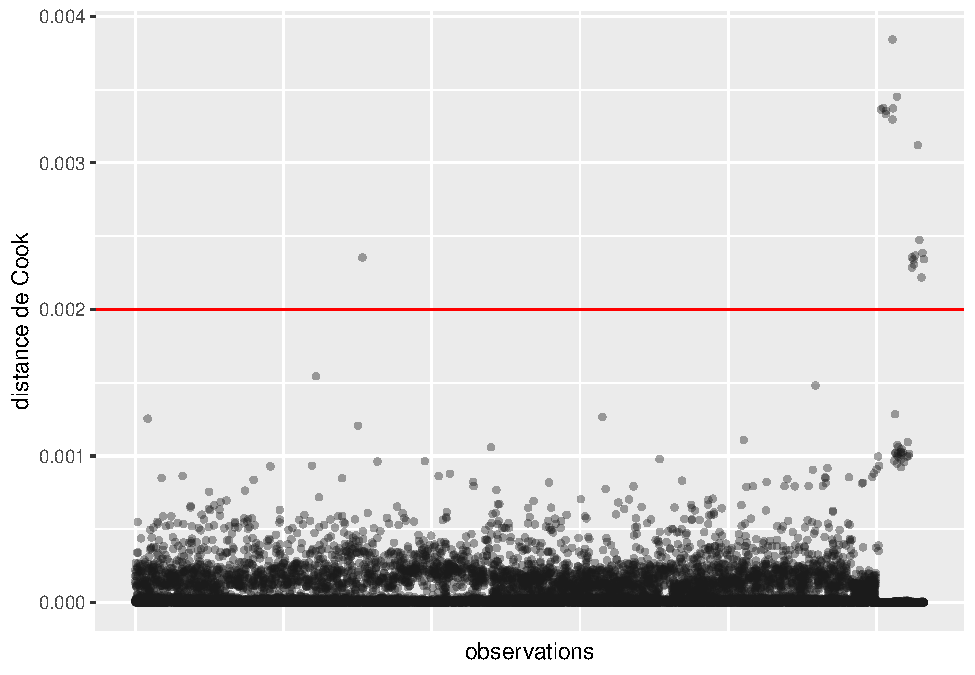
\includegraphics{livre_statistique_Phil_Jere_clean_files/figure-latex/unnamed-chunk-5-1.pdf}

\begin{Shaded}
\begin{Highlighting}[]
\KeywordTok{barplot}\NormalTok{(res.acp}\OperatorTok{$}\NormalTok{eig[,}\DecValTok{2}\NormalTok{], }\DataTypeTok{main=}\StringTok{"Variance expliquée (%)"}\NormalTok{, }\DataTypeTok{names.arg=}\DecValTok{1}\OperatorTok{:}\KeywordTok{nrow}\NormalTok{(res.acp}\OperatorTok{$}\NormalTok{eig))}
\end{Highlighting}
\end{Shaded}

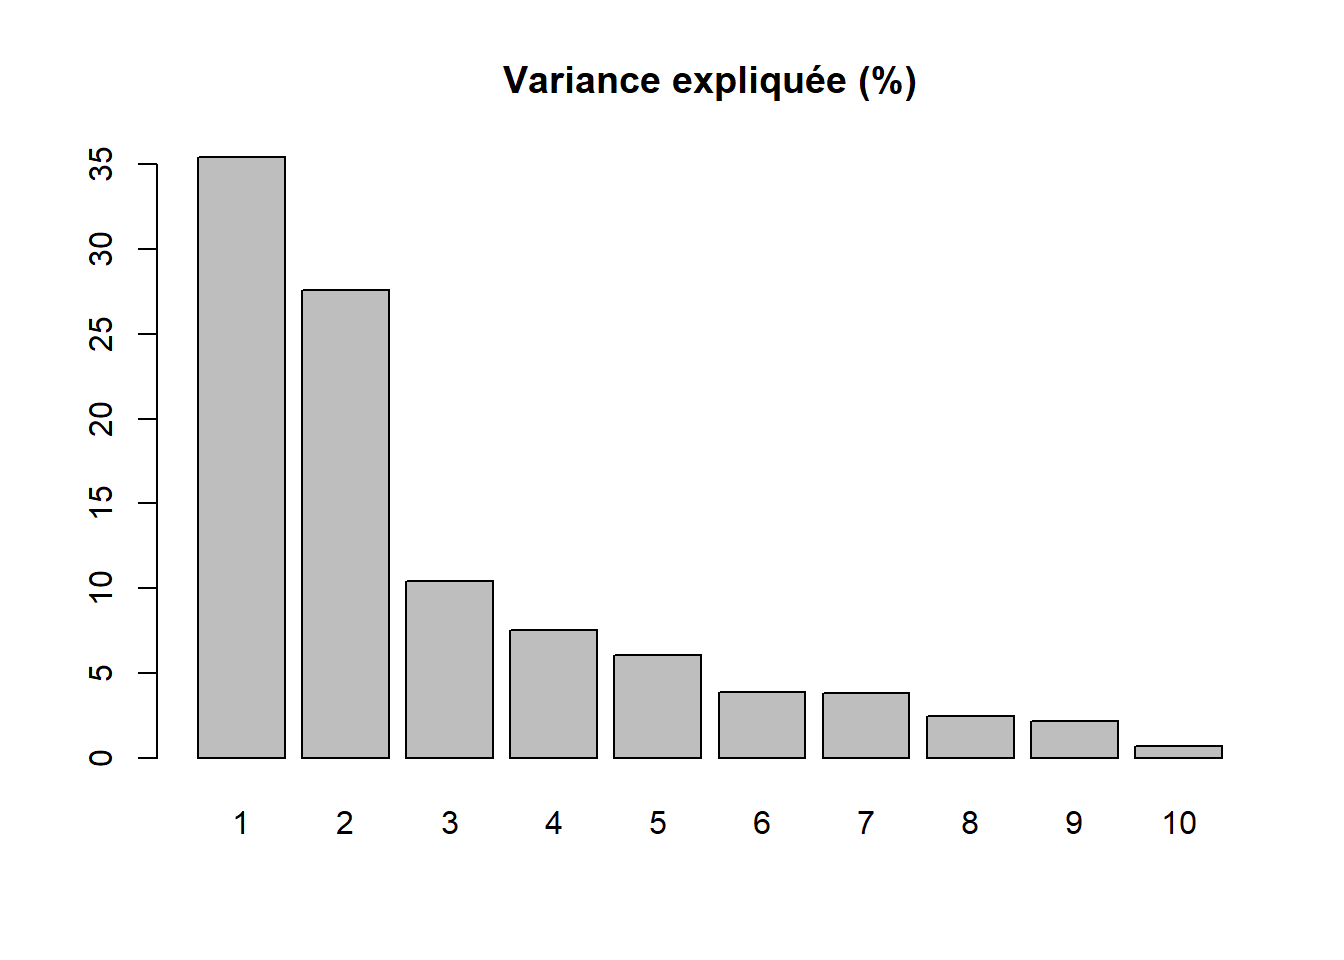
\includegraphics{livre_statistique_Phil_Jere_clean_files/figure-latex/unnamed-chunk-5-2.pdf}

\begin{Shaded}
\begin{Highlighting}[]
\KeywordTok{barplot}\NormalTok{(res.acp}\OperatorTok{$}\NormalTok{eig[,}\DecValTok{3}\NormalTok{], }\DataTypeTok{main=}\StringTok{"Variance expliquée cumulée (%)"}\NormalTok{,}
        \DataTypeTok{names.arg=}\DecValTok{1}\OperatorTok{:}\KeywordTok{nrow}\NormalTok{(res.acp}\OperatorTok{$}\NormalTok{eig))}
\end{Highlighting}
\end{Shaded}

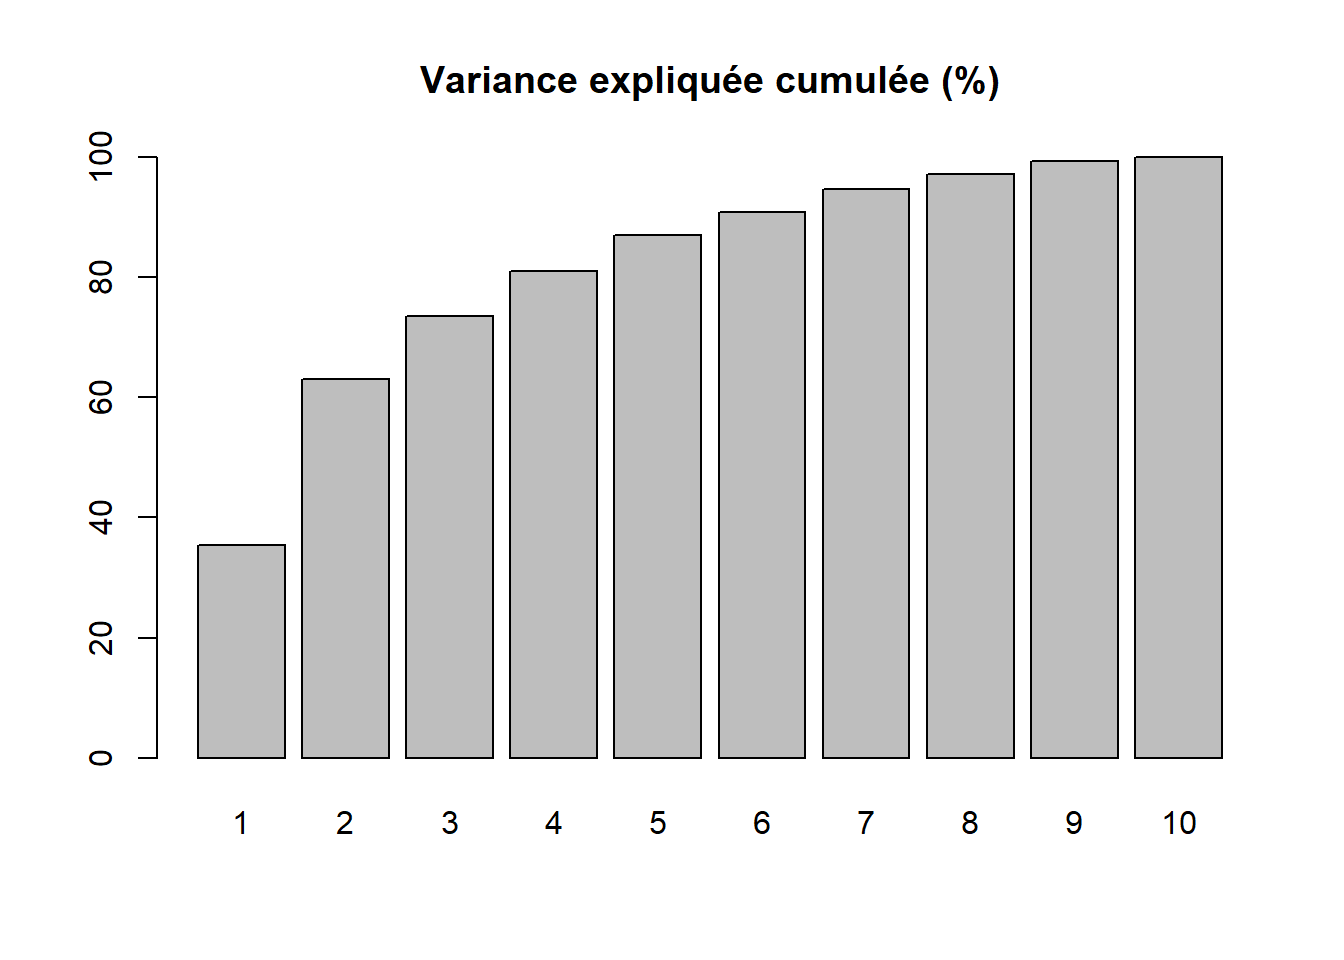
\includegraphics{livre_statistique_Phil_Jere_clean_files/figure-latex/unnamed-chunk-5-3.pdf}

\begin{Shaded}
\begin{Highlighting}[]
\CommentTok{# Nuage du points du premier plan factoriel pour les variables et les individus}
\KeywordTok{plot}\NormalTok{(res.acp, }\DataTypeTok{graph.type =} \StringTok{"classic"}\NormalTok{, }\DataTypeTok{choix=}\StringTok{"var"}\NormalTok{, }\DataTypeTok{axes =} \DecValTok{1}\OperatorTok{:}\DecValTok{2}\NormalTok{, }
     \DataTypeTok{title =} \StringTok{"Premier plan factoriel (variables)"}\NormalTok{)}
\end{Highlighting}
\end{Shaded}

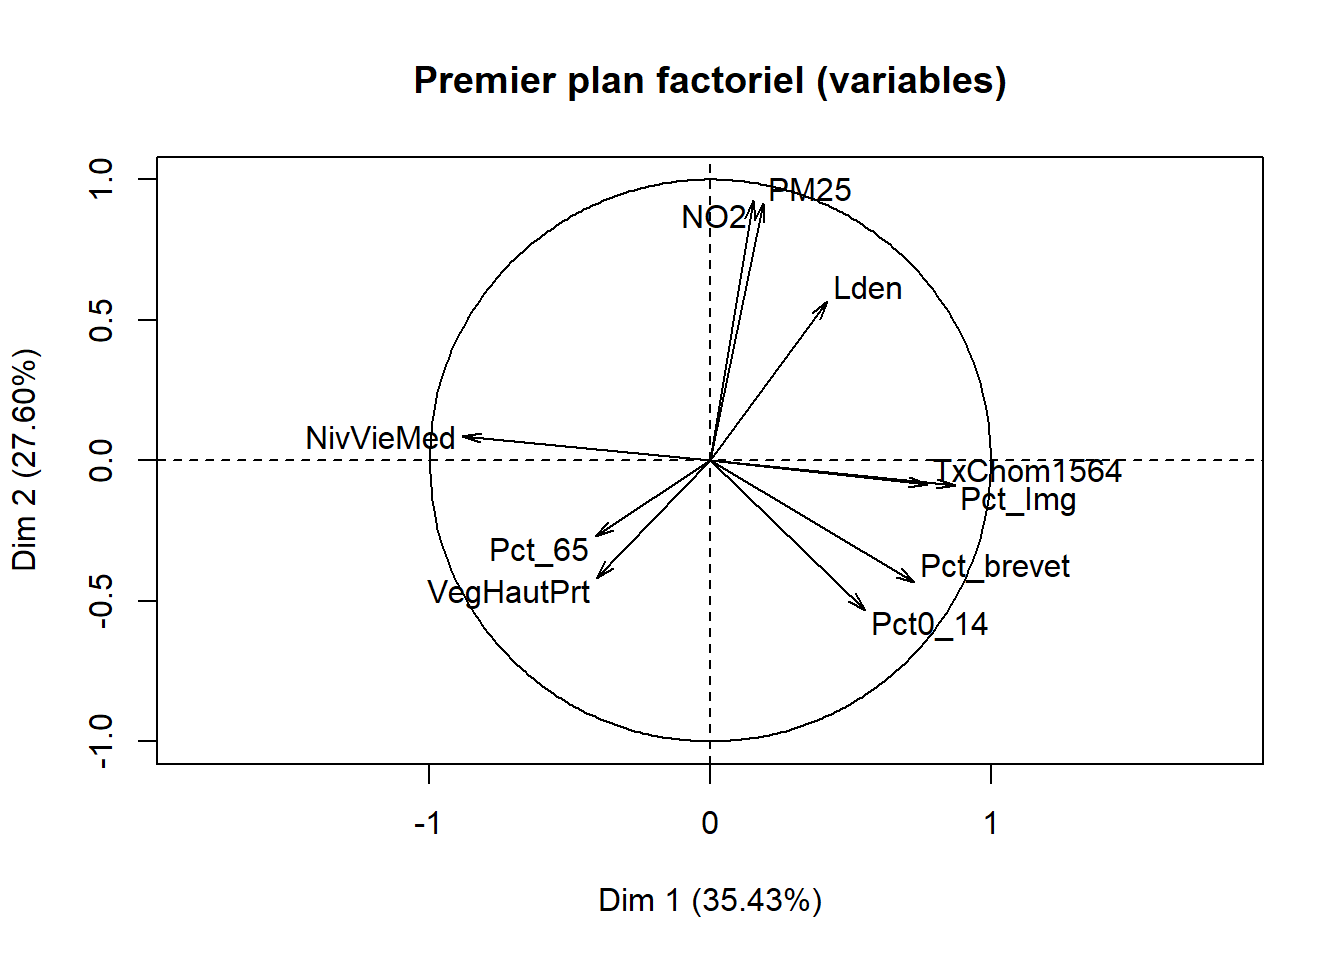
\includegraphics{livre_statistique_Phil_Jere_clean_files/figure-latex/unnamed-chunk-5-4.pdf}

\begin{Shaded}
\begin{Highlighting}[]
\KeywordTok{plot}\NormalTok{(res.acp, }\DataTypeTok{graph.type =} \StringTok{"classic"}\NormalTok{, }\DataTypeTok{choix=}\StringTok{"ind"}\NormalTok{, }\DataTypeTok{axes =} \DecValTok{1}\OperatorTok{:}\DecValTok{2}\NormalTok{, }
     \DataTypeTok{title =} \StringTok{"Premier plan factoriel (individus)"}\NormalTok{)}
\end{Highlighting}
\end{Shaded}

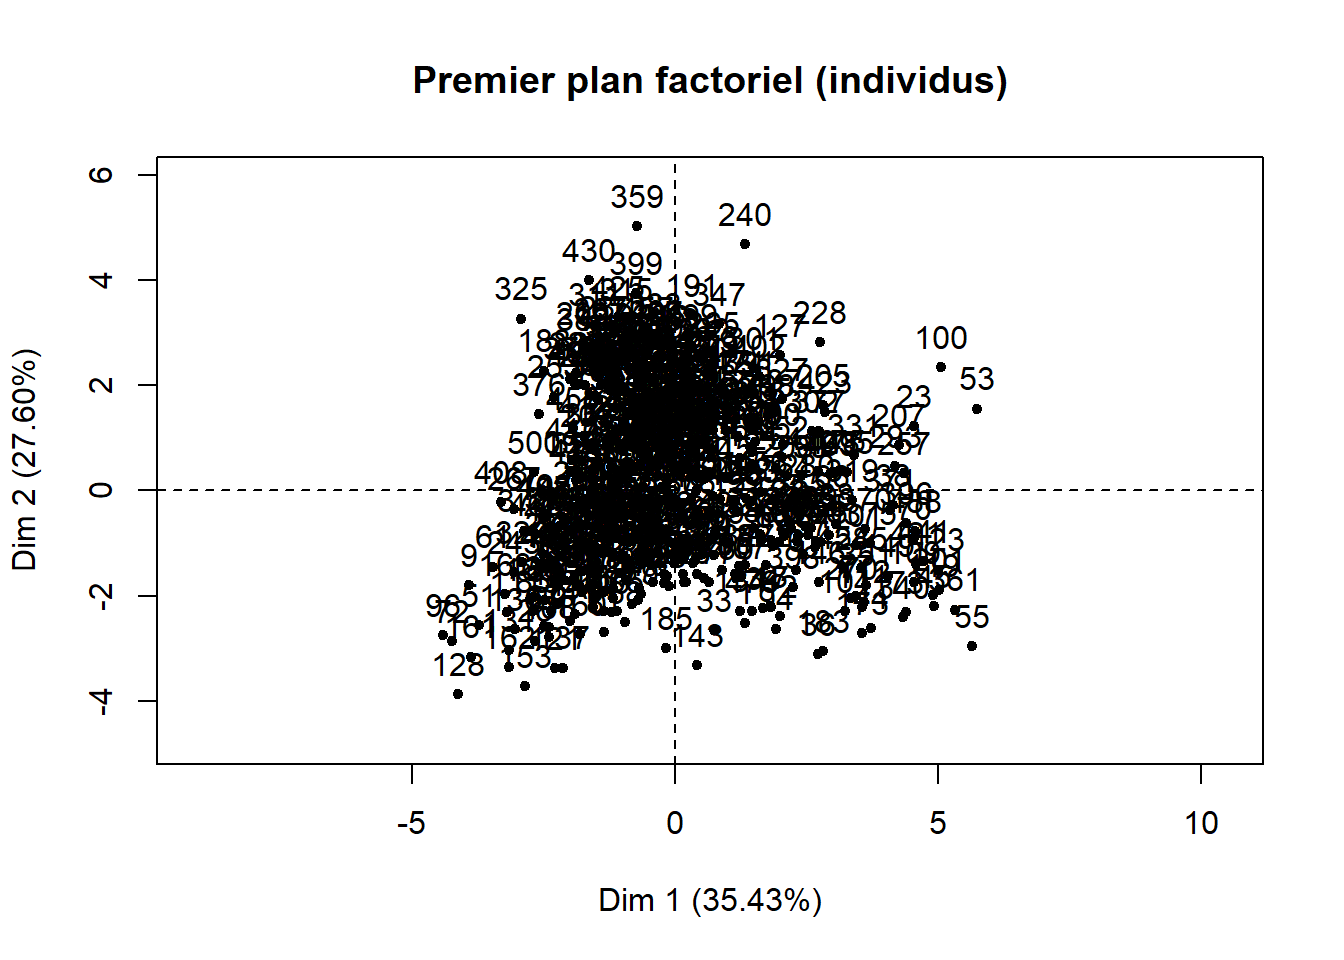
\includegraphics{livre_statistique_Phil_Jere_clean_files/figure-latex/unnamed-chunk-5-5.pdf}

\begin{bloc_aller_loin}
Nous avons vu dans un encadré ci-dessus qu'il est possible d'ajouter des variables et des individus supplémentaires dans une ACP, ce que permet la fonction \texttt{PCA} de \texttt{FactoMineR} avec les paramètres \texttt{ind.sup} et \texttt{quanti.sup}. Aussi, pour ajouter des pondérations aux individus ou aux variables, utilisez les paramètres \texttt{row.w} et \texttt{col.w}. Pour plus d'informations sur ces paramètres, consulter l'aide de la fonction en tapant \texttt{?PCA} dans la console de Rstudio.

\end{bloc_aller_loin}

\hypertarget{sect12232}{%
\subsubsection{\texorpdfstring{Exploration graphique des résultats de l'ACP avec \texttt{factoextra}}{Exploration graphique des résultats de l'ACP avec factoextra}}\label{sect12232}}

Visuellement, vous avez pu constater que les graphiques ci-dessus (pour les valeurs propres et pour le premier plan factoriel pour les variables et les individus) réalisés avec les fonctions de base \texttt{barplot} et \texttt{plot} sont peu attrayants. Avec le \emph{package} \texttt{factoextra}, quelques lignes de code suffissent pour construire des graphiques bien plus esthétiques.

Premièrement, la syntaxe ci-dessous renvoie deux graphiques pour analyser les résultats des valeurs propres (figure~\ref{fig:factoextra1}).

\begin{Shaded}
\begin{Highlighting}[]
\KeywordTok{library}\NormalTok{(factoextra)}
\KeywordTok{library}\NormalTok{(ggplot2)}
\KeywordTok{library}\NormalTok{(ggpubr)}

\CommentTok{# Graphiques pour les variables propres avec factoextra}
\NormalTok{G1 <-}\StringTok{ }\KeywordTok{fviz_screeplot}\NormalTok{(res.acp, }\DataTypeTok{choice =}\StringTok{"eigenvalue"}\NormalTok{, }\DataTypeTok{addlabels =} \OtherTok{TRUE}\NormalTok{,}
                     \DataTypeTok{x=}\StringTok{"Composantes"}\NormalTok{,}
                     \DataTypeTok{y=}\StringTok{"Valeur propre"}\NormalTok{,}
                    \DataTypeTok{title=}\StringTok{""}\NormalTok{)}
\NormalTok{G2 <-}\StringTok{ }\KeywordTok{fviz_screeplot}\NormalTok{(res.acp, }\DataTypeTok{choice =}\StringTok{"variance"}\NormalTok{, }\DataTypeTok{addlabels =} \OtherTok{TRUE}\NormalTok{,}
                     \DataTypeTok{x=}\StringTok{"Composantes"}\NormalTok{,}
                     \DataTypeTok{y=}\StringTok{"Pourcentage de la variance expliquée"}\NormalTok{,}
                     \DataTypeTok{title=}\StringTok{""}\NormalTok{)}
\KeywordTok{ggarrange}\NormalTok{(G1, G2)}
\end{Highlighting}
\end{Shaded}

\begin{figure}

{\centering 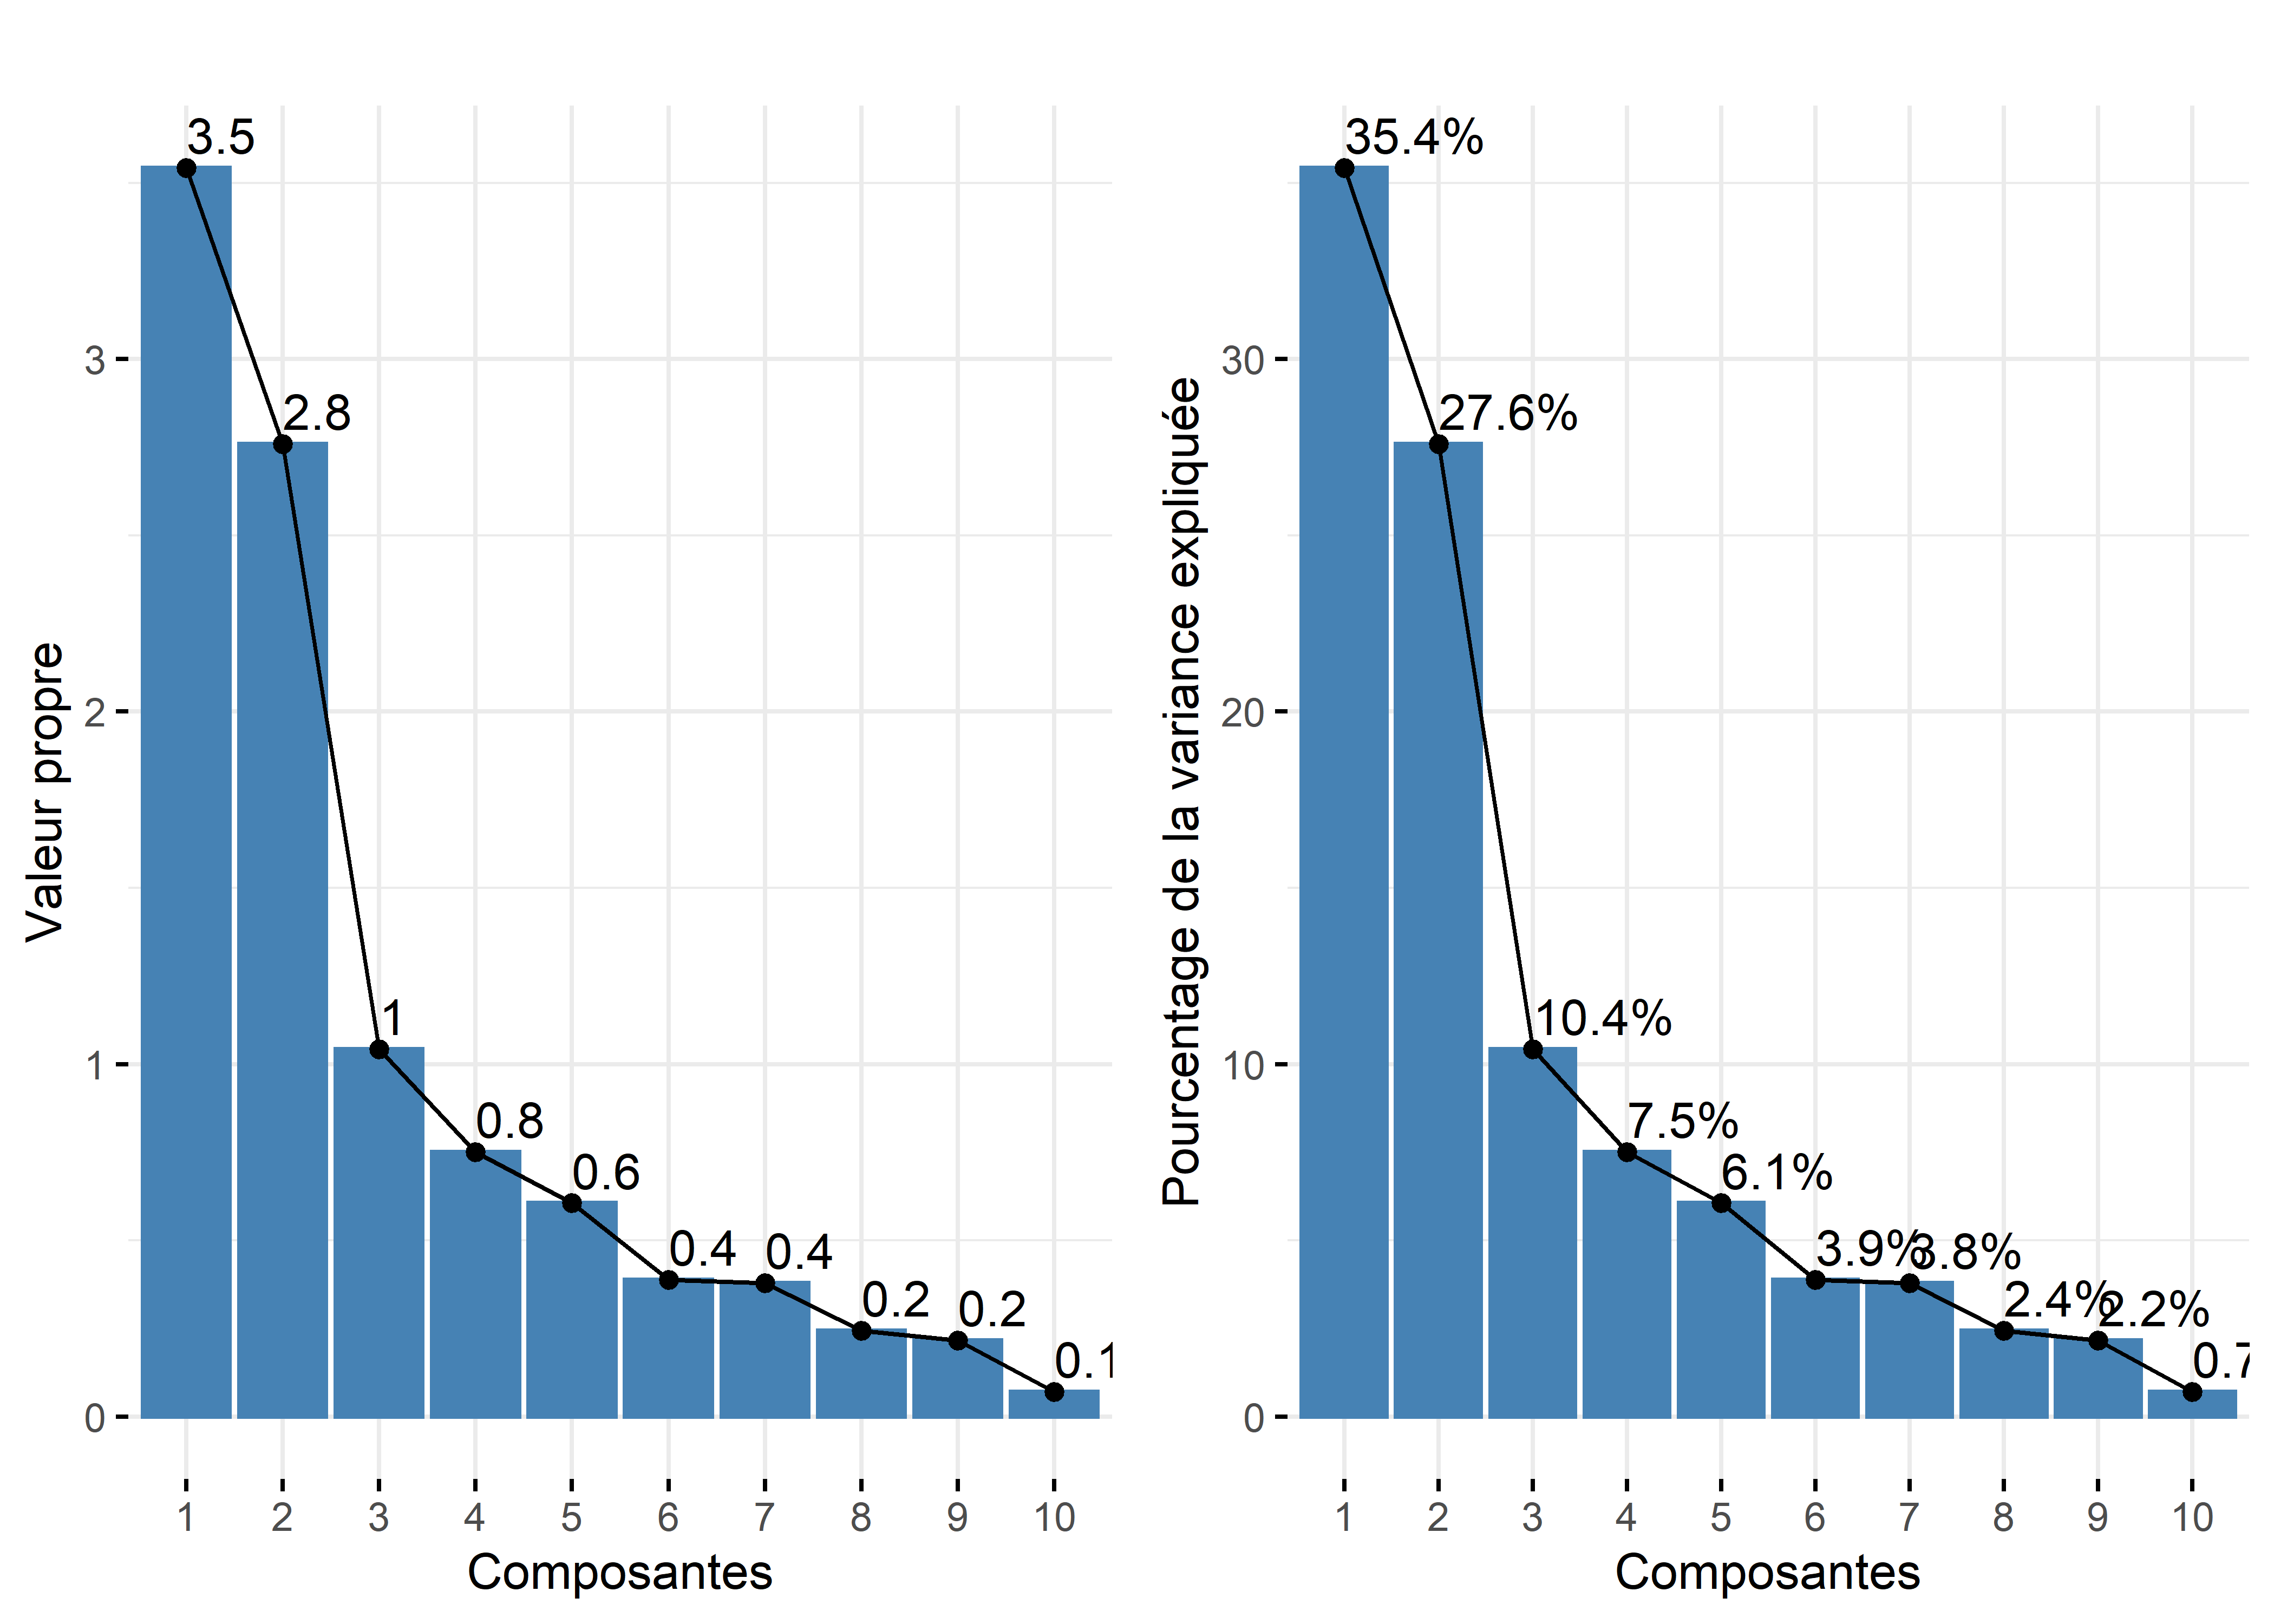
\includegraphics[width=0.75\linewidth]{livre_statistique_Phil_Jere_clean_files/figure-latex/factoextra1-1} 

}

\caption{Graphiques pour les valeurs propres de l'ACP avec factoextra}\label{fig:factoextra1}
\end{figure}

Deuxièmement, la syntaxe ci-dessous renvoie trois graphiques pour analyser les contributions de chaque variable aux deux premiers axes de l'ACP (figures \ref{fig:factoextra2} et \ref{fig:factoextra3}) et la qualité de représentation des variables sur les trois premiers axes (figure~\ref{fig:factoextra4}), c'est-à-dire la somme des cosinus carrés sur les trois axes retenus.

\begin{Shaded}
\begin{Highlighting}[]
\CommentTok{# Contributions des variables aux deux premières composantes avec factoextra}
\KeywordTok{fviz_contrib}\NormalTok{(res.acp, }\DataTypeTok{choice =} \StringTok{"var"}\NormalTok{, }\DataTypeTok{axes =} \DecValTok{1}\NormalTok{, }\DataTypeTok{top =} \DecValTok{10}\NormalTok{,}
             \DataTypeTok{title =} \StringTok{"Contributions des variables à la première composante"}\NormalTok{)}
\KeywordTok{fviz_contrib}\NormalTok{(res.acp, }\DataTypeTok{choice =} \StringTok{"var"}\NormalTok{, }\DataTypeTok{axes =} \DecValTok{2}\NormalTok{, }\DataTypeTok{top =} \DecValTok{10}\NormalTok{,}
             \DataTypeTok{title =} \StringTok{"Contributions des variables à la première composante"}\NormalTok{)}
\KeywordTok{fviz_cos2}\NormalTok{(res.acp, }\DataTypeTok{choice =} \StringTok{"var"}\NormalTok{, }\DataTypeTok{axes =} \DecValTok{1}\OperatorTok{:}\DecValTok{3}\NormalTok{)}\OperatorTok{+}
\StringTok{  }\KeywordTok{labs}\NormalTok{(}\DataTypeTok{x=}\StringTok{""}\NormalTok{, }\DataTypeTok{y=}\StringTok{"Somme des cosinus carrés sur les 3 axes retenus"}\NormalTok{,}
       \DataTypeTok{title =}\StringTok{"Qualité de représentation des variables sur les axes retenus de l'ACP"}\NormalTok{)}
\end{Highlighting}
\end{Shaded}

\begin{figure}

{\centering 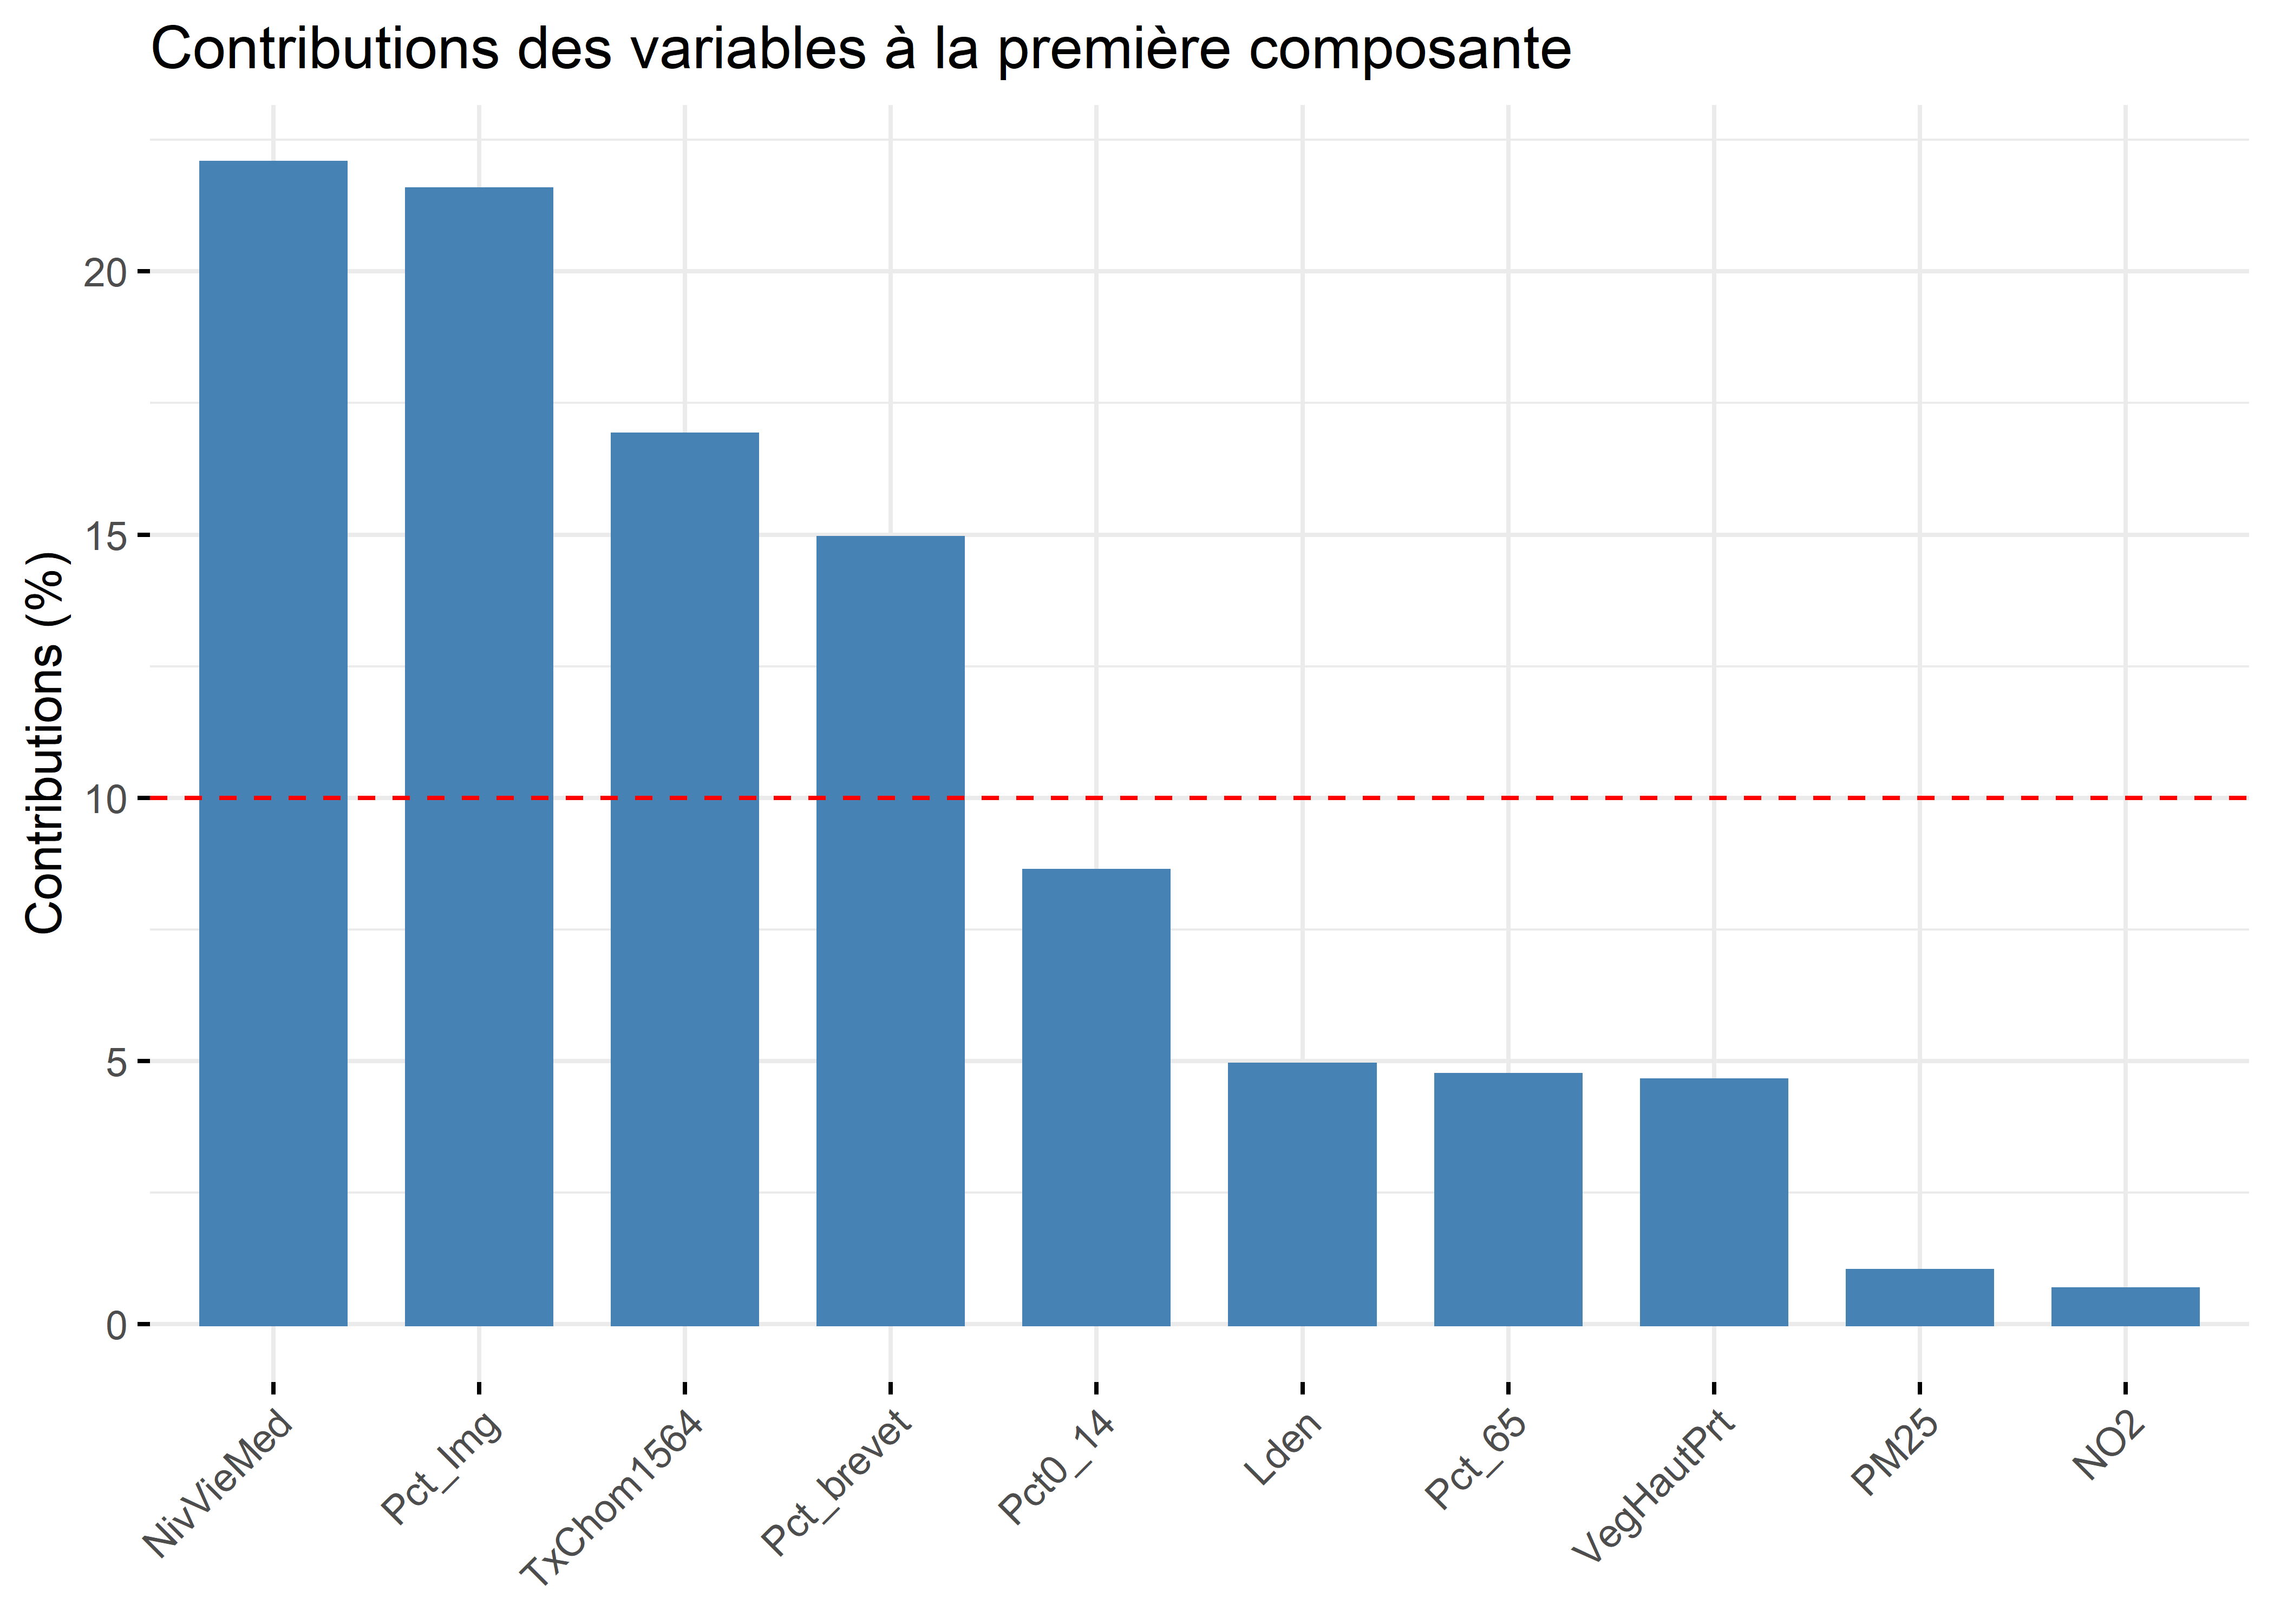
\includegraphics[width=0.85\linewidth]{livre_statistique_Phil_Jere_clean_files/figure-latex/factoextra2-1} 

}

\caption{Contributions des variables à la première composante avec factoextra}\label{fig:factoextra2}
\end{figure}

\begin{figure}

{\centering 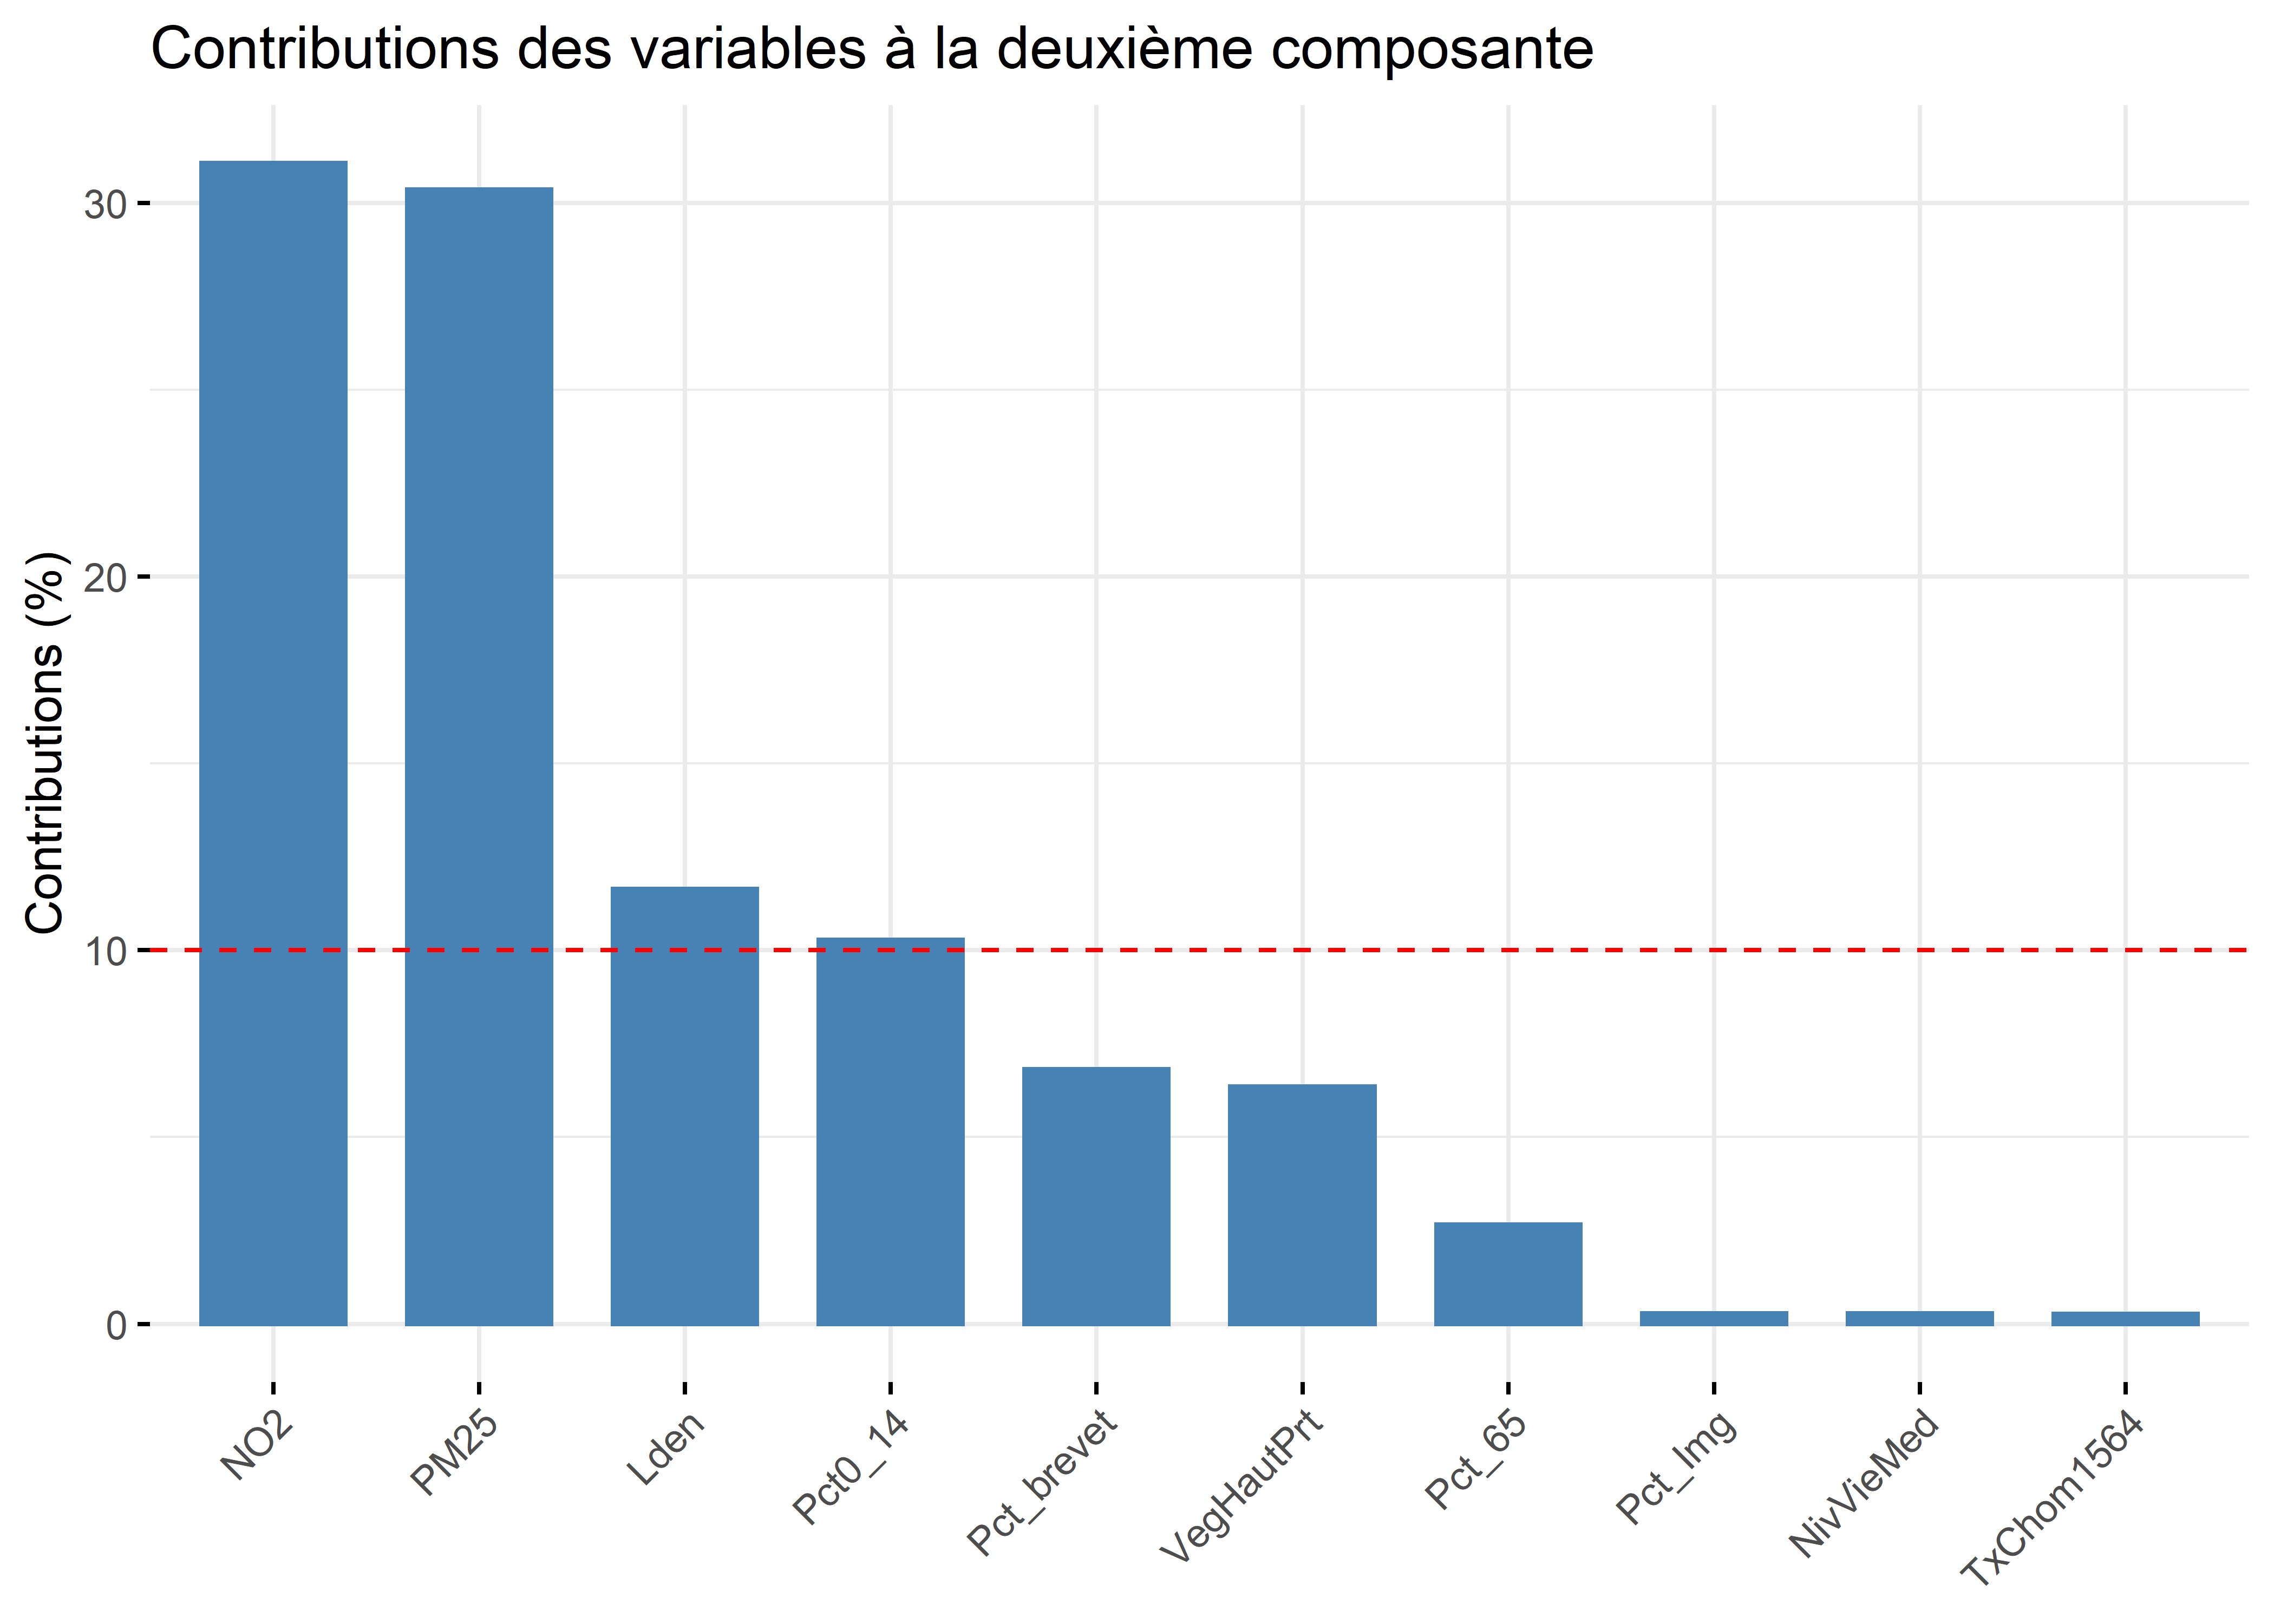
\includegraphics[width=0.85\linewidth]{livre_statistique_Phil_Jere_clean_files/figure-latex/factoextra3-1} 

}

\caption{Contributions des variables à la deuxième composante avec factoextra}\label{fig:factoextra3}
\end{figure}

\begin{figure}

{\centering 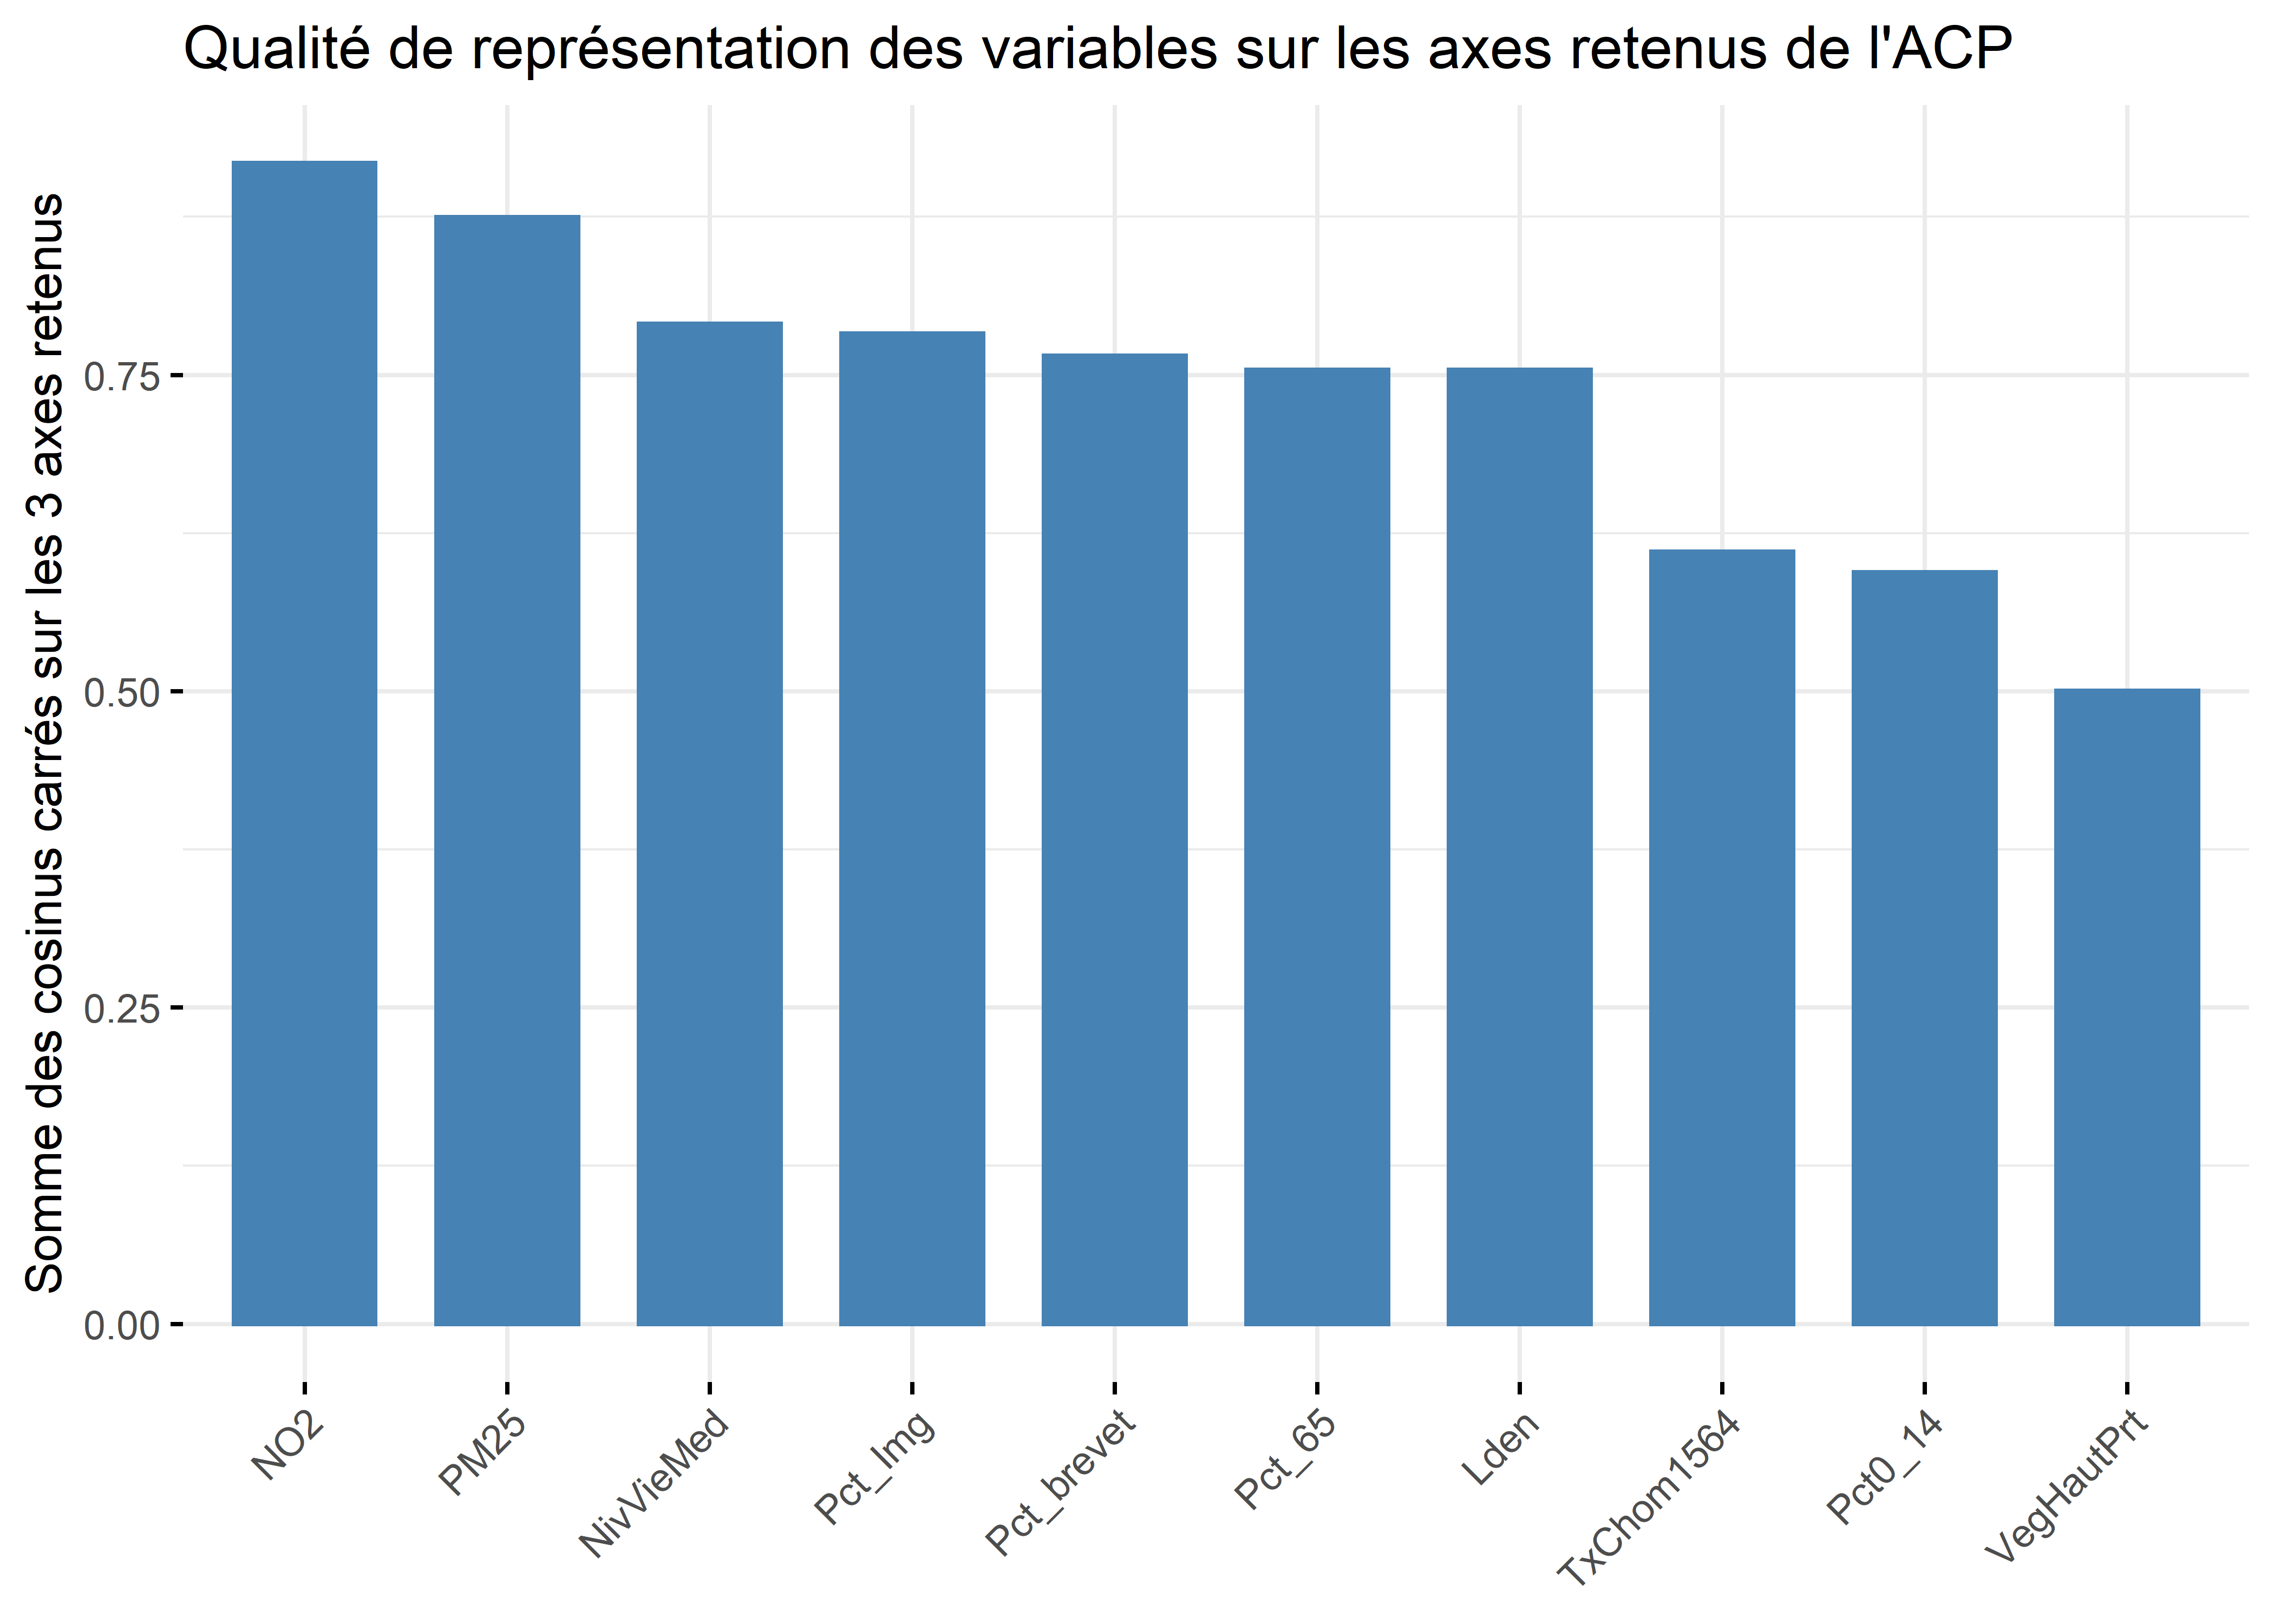
\includegraphics[width=0.85\linewidth]{livre_statistique_Phil_Jere_clean_files/figure-latex/factoextra4-1} 

}

\caption{Qualité des variables sur les trois premières composantes avec factoextra}\label{fig:factoextra4}
\end{figure}

Troisièmement, le code ci-dessous renvoie un nuage de points pour le premier plan factoriel de l'ACP (axes 1 et 2) pour les variables (figure~\ref{fig:factoextra5}) et les individus (figure~\ref{fig:factoextra6}).

\begin{Shaded}
\begin{Highlighting}[]
\CommentTok{# Premier plan factoriel pour les variables avec factoextra}
\KeywordTok{fviz_pca_var}\NormalTok{(res.acp, }\DataTypeTok{col.var=}\StringTok{"contrib"}\NormalTok{,}
             \DataTypeTok{title =} \StringTok{"Premier plan factoriel pour les variables"}\NormalTok{)}\OperatorTok{+}
\StringTok{  }\KeywordTok{scale_color_gradient2}\NormalTok{(}\DataTypeTok{low=}\StringTok{"#313695"}\NormalTok{, }\DataTypeTok{mid=}\StringTok{"#ffffbf"}\NormalTok{, }\DataTypeTok{high=}\StringTok{"#a50026"}\NormalTok{,}
                        \DataTypeTok{midpoint=}\KeywordTok{mean}\NormalTok{(res.acp}\OperatorTok{$}\NormalTok{var}\OperatorTok{$}\NormalTok{contrib[,}\DecValTok{1}\NormalTok{]))}
\CommentTok{# Premier plan factoriel pour les individus avec factoextra}
\KeywordTok{fviz_pca_ind}\NormalTok{(res.acp, }\DataTypeTok{label=}\StringTok{"none"}\NormalTok{)}
\KeywordTok{fviz_pca_ind}\NormalTok{(res.acp, }\DataTypeTok{col.ind=}\StringTok{"cos2"}\NormalTok{) }\OperatorTok{+}
\StringTok{  }\KeywordTok{scale_color_gradient2}\NormalTok{(}\DataTypeTok{low=}\StringTok{"blue"}\NormalTok{, }\DataTypeTok{mid=}\StringTok{"white"}\NormalTok{, }\DataTypeTok{high=}\StringTok{"red"}\NormalTok{, }\DataTypeTok{midpoint=}\FloatTok{0.50}\NormalTok{)}
\end{Highlighting}
\end{Shaded}

\begin{figure}

{\centering 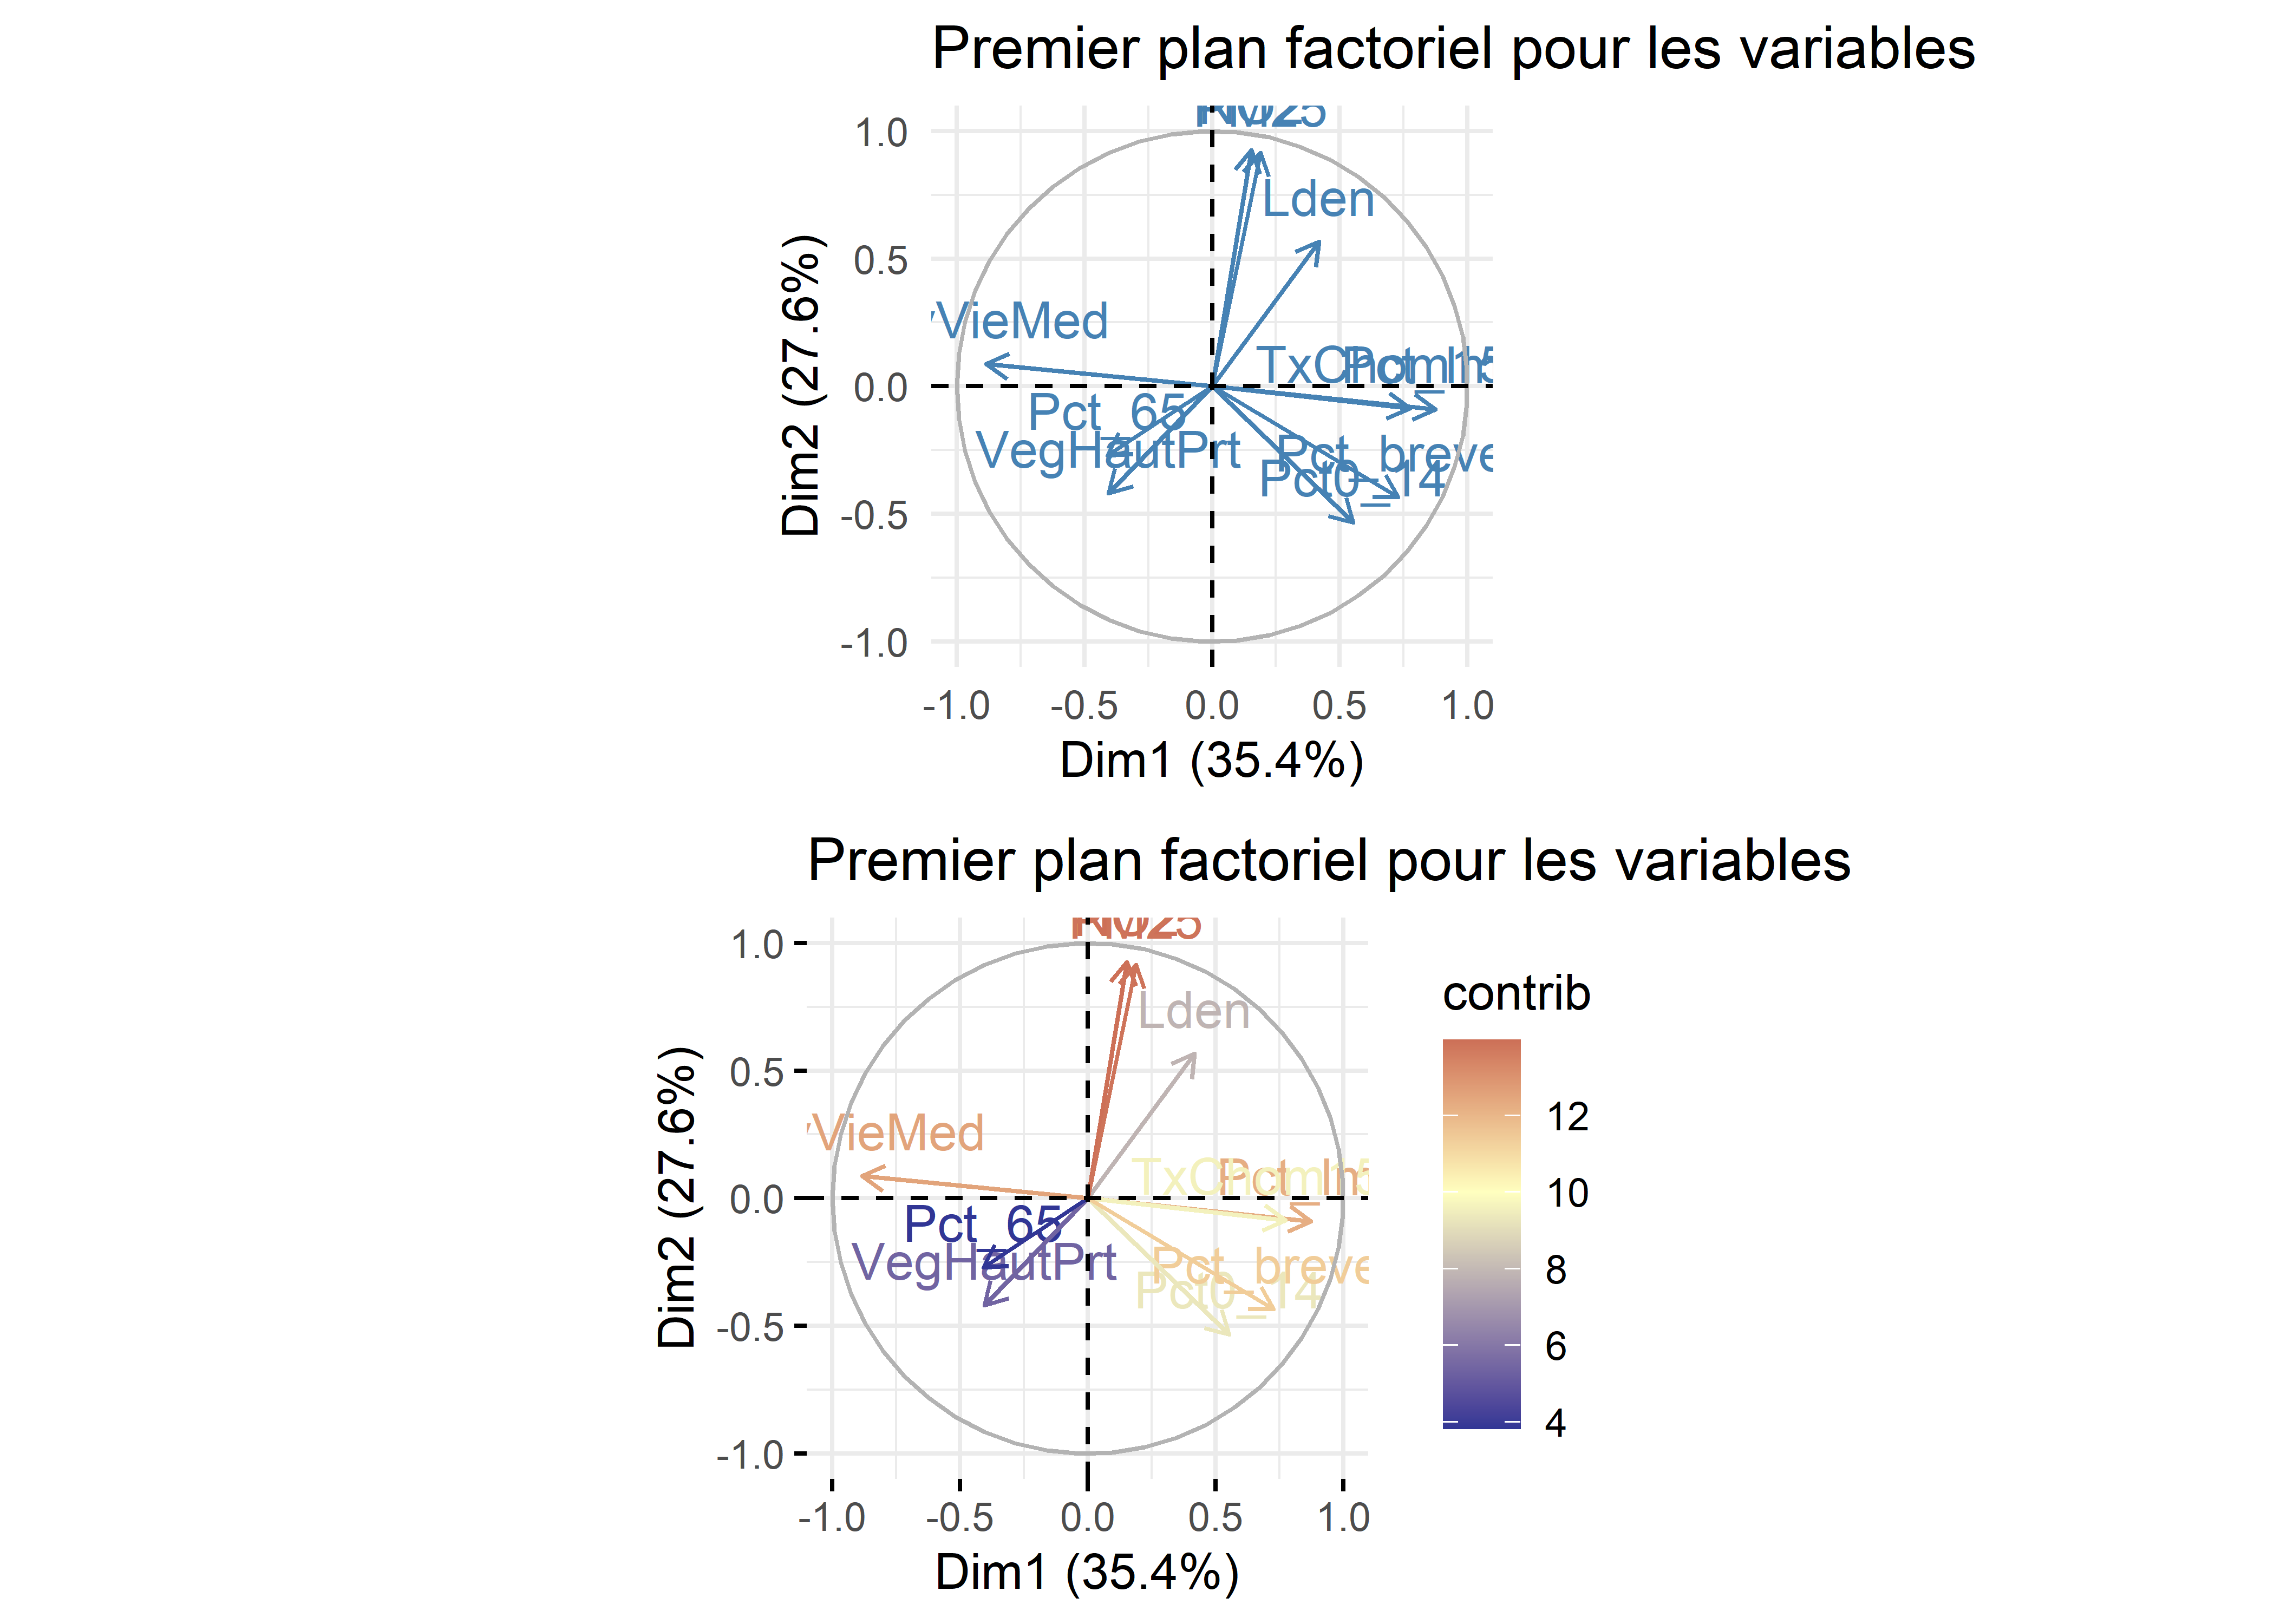
\includegraphics[width=1\linewidth]{livre_statistique_Phil_Jere_clean_files/figure-latex/factoextra5-1} 

}

\caption{Premier plan factoriel de l'ACP pour les variables avec factoextra}\label{fig:factoextra5}
\end{figure}

\begin{figure}

{\centering 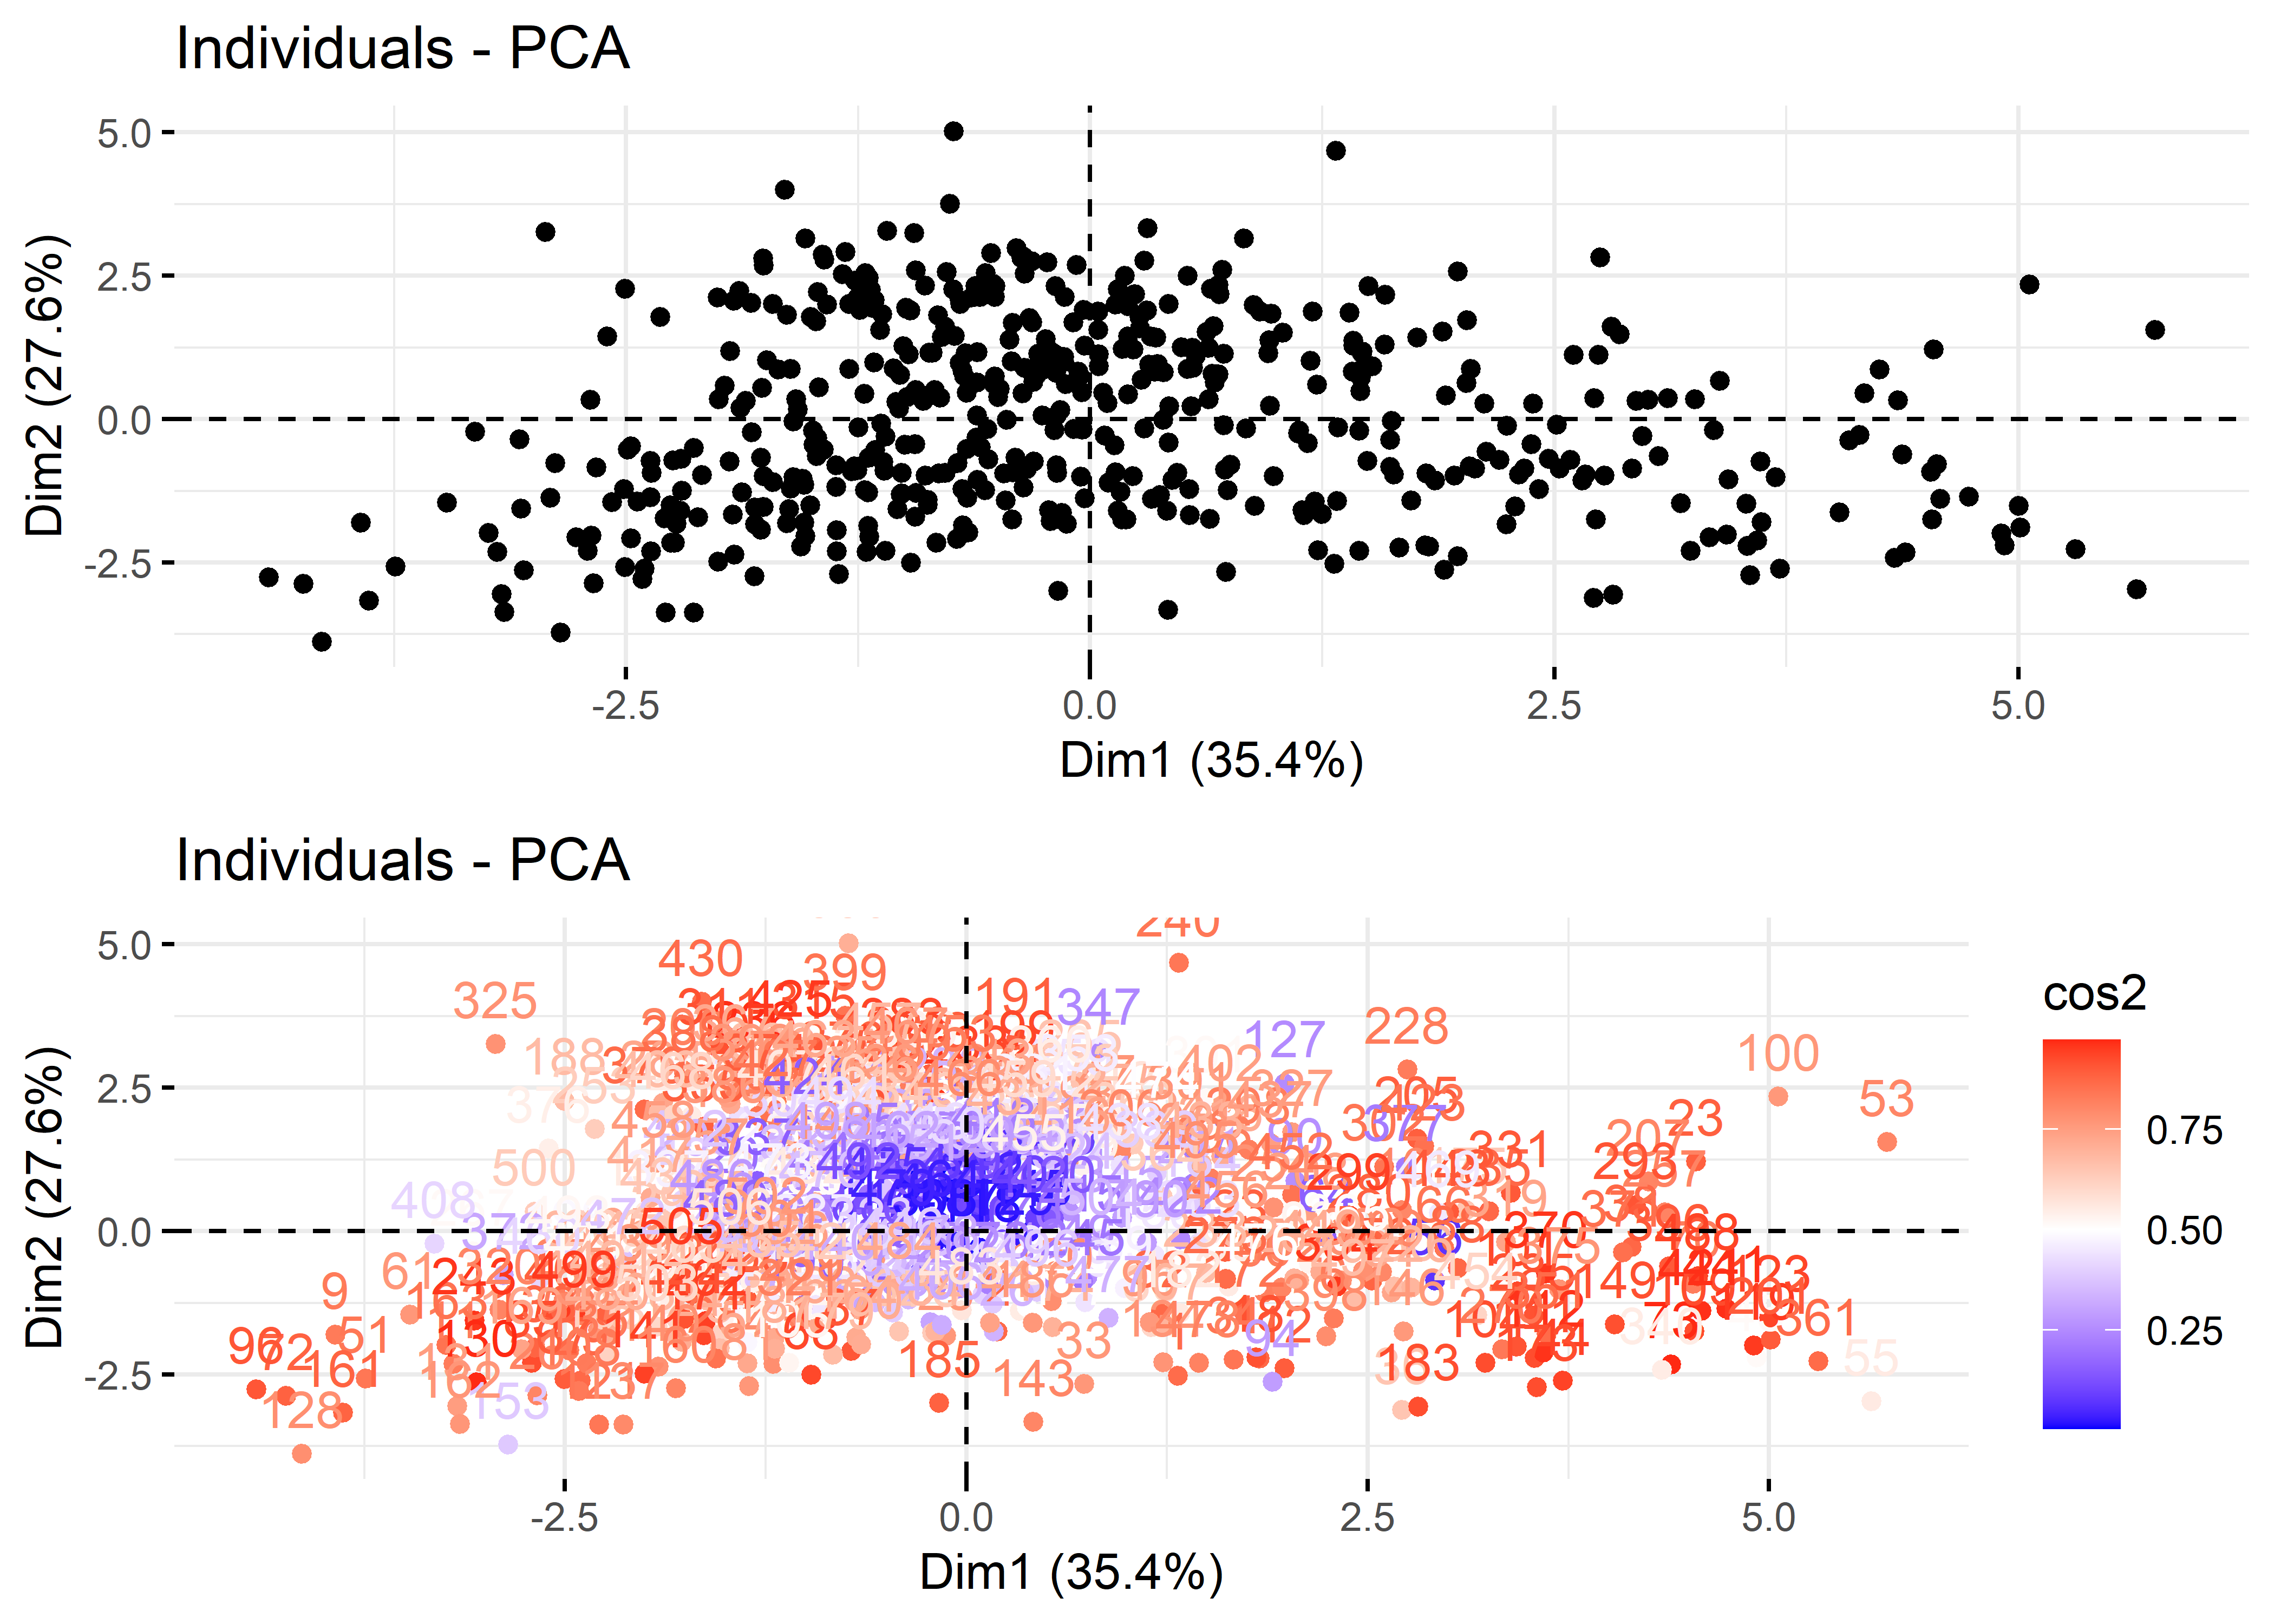
\includegraphics[width=0.75\linewidth]{livre_statistique_Phil_Jere_clean_files/figure-latex/factoextra6-1} 

}

\caption{Premier plan factoriel de l'ACP pour les individus avec factoextra}\label{fig:factoextra6}
\end{figure}

\hypertarget{sect12233}{%
\subsubsection{Personnalisation des graphiques avec les résultats de l'ACP}\label{sect12233}}

Avec un peu plus de code et l'utilisation d'autres \emph{packages} (\texttt{ggplot2}, \texttt{ggpubr}, \texttt{stringr}, \texttt{corrplot}), vous pouvez aussi construire des graphiques personnalisés.

Premièrement, la syntaxe ci-dessous permet de réaliser trois graphiques pour analyser les valeurs propres (figure~\ref{fig:acpmesgraphs1}). Notez que, d'un coup d'œil, nous pouvons identifier les composantes principales avec une valeur propre égale ou supérieure à 1.

\begin{Shaded}
\begin{Highlighting}[]
\KeywordTok{library}\NormalTok{(ggplot2)}
\KeywordTok{library}\NormalTok{(ggpubr)}
\KeywordTok{library}\NormalTok{(stringr)}
\KeywordTok{library}\NormalTok{(corrplot)}

\CommentTok{# Calcul de l'ACP}
\NormalTok{res.acp <-}\StringTok{ }\KeywordTok{PCA}\NormalTok{(Data[,}\DecValTok{2}\OperatorTok{:}\DecValTok{11}\NormalTok{], }\DataTypeTok{ncp=}\DecValTok{5}\NormalTok{, }\DataTypeTok{scale.unit=}\OtherTok{TRUE}\NormalTok{, }\DataTypeTok{graph=}\NormalTok{F)}
\KeywordTok{print}\NormalTok{(res.acp)}

\CommentTok{# Construction d'un dataframe pour les valeurs propres}
\NormalTok{dfACPvp <-}\StringTok{ }\KeywordTok{data.frame}\NormalTok{(res.acp}\OperatorTok{$}\NormalTok{eig)}
\KeywordTok{names}\NormalTok{(dfACPvp) <-}\StringTok{ }\KeywordTok{c}\NormalTok{(}\StringTok{"VP"}\NormalTok{,}\StringTok{"VP_pct"}\NormalTok{,}\StringTok{"VP_cumupct"}\NormalTok{)}
\NormalTok{dfACPvp}\OperatorTok{$}\NormalTok{Composante <-}\StringTok{ }\KeywordTok{factor}\NormalTok{(}\DecValTok{1}\OperatorTok{:}\KeywordTok{nrow}\NormalTok{(dfACPvp), }\DataTypeTok{levels=}\KeywordTok{rev}\NormalTok{(}\DecValTok{1}\OperatorTok{:}\KeywordTok{nrow}\NormalTok{(dfACPvp)))}
\NormalTok{couleursAxes <-}\StringTok{ }\KeywordTok{c}\NormalTok{(}\StringTok{"steelblue"}\NormalTok{,}\StringTok{"skyblue2"}\NormalTok{)}
\NormalTok{vpsup1 <-}\StringTok{ }\KeywordTok{round}\NormalTok{(}\KeywordTok{sum}\NormalTok{(}\KeywordTok{subset}\NormalTok{(dfACPvp, VP }\OperatorTok{>=}\StringTok{ }\DecValTok{1}\NormalTok{)}\OperatorTok{$}\NormalTok{VP),}\DecValTok{2}\NormalTok{)}
\NormalTok{vpsup1cumul <-}\StringTok{ }\KeywordTok{round}\NormalTok{(}\KeywordTok{sum}\NormalTok{(}\KeywordTok{subset}\NormalTok{(dfACPvp, VP }\OperatorTok{>=}\StringTok{ }\DecValTok{1}\NormalTok{)}\OperatorTok{$}\NormalTok{VP_pct),}\DecValTok{2}\NormalTok{)}

\NormalTok{plotVP1 <-}\StringTok{ }\KeywordTok{ggplot}\NormalTok{(dfACPvp,}\KeywordTok{aes}\NormalTok{(}\DataTypeTok{x=}\NormalTok{VP, }\DataTypeTok{y=}\NormalTok{Composante,}\DataTypeTok{fill=}\NormalTok{VP}\OperatorTok{<}\DecValTok{1}\NormalTok{))}\OperatorTok{+}
\StringTok{  }\KeywordTok{geom_bar}\NormalTok{(}\DataTypeTok{stat=}\StringTok{"identity"}\NormalTok{, }\DataTypeTok{width =} \FloatTok{.6}\NormalTok{, }\DataTypeTok{alpha=}\NormalTok{.}\DecValTok{8}\NormalTok{, }\DataTypeTok{color=}\StringTok{"black"}\NormalTok{)}\OperatorTok{+}
\StringTok{  }\KeywordTok{geom_vline}\NormalTok{(}\DataTypeTok{xintercept=}\DecValTok{1}\NormalTok{, }\DataTypeTok{linetype=}\StringTok{"dashed"}\NormalTok{, }\DataTypeTok{color =} \StringTok{"azure4"}\NormalTok{, }\DataTypeTok{size=}\DecValTok{1}\NormalTok{)}\OperatorTok{+}
\StringTok{  }\KeywordTok{scale_fill_manual}\NormalTok{(}\DataTypeTok{name=}\StringTok{"Valeur}\CharTok{\textbackslash{}n}\StringTok{propre"}\NormalTok{,}\DataTypeTok{values=}\NormalTok{couleursAxes,}\DataTypeTok{labels =} \KeywordTok{c}\NormalTok{(}\StringTok{">= 1"}\NormalTok{,}\StringTok{"< 1"}\NormalTok{))}\OperatorTok{+}
\StringTok{  }\KeywordTok{labs}\NormalTok{(}\DataTypeTok{x=}\StringTok{"Valeur propre"}\NormalTok{, }\DataTypeTok{y=}\StringTok{"Composante principale"}\NormalTok{)}
\NormalTok{plotVP2 <-}\StringTok{ }\KeywordTok{ggplot}\NormalTok{(dfACPvp, }\KeywordTok{aes}\NormalTok{(}\DataTypeTok{x=}\NormalTok{VP_pct, }\DataTypeTok{y=}\NormalTok{Composante,}\DataTypeTok{fill=}\NormalTok{VP}\OperatorTok{<}\DecValTok{1}\NormalTok{))}\OperatorTok{+}
\StringTok{  }\KeywordTok{geom_bar}\NormalTok{(}\DataTypeTok{stat=}\StringTok{"identity"}\NormalTok{, }\DataTypeTok{width =} \FloatTok{.6}\NormalTok{, }\DataTypeTok{alpha=}\NormalTok{.}\DecValTok{8}\NormalTok{, }\DataTypeTok{color=}\StringTok{"black"}\NormalTok{)}\OperatorTok{+}
\StringTok{  }\KeywordTok{scale_fill_manual}\NormalTok{(}\DataTypeTok{name=}\StringTok{"Valeur}\CharTok{\textbackslash{}n}\StringTok{propre"}\NormalTok{,}\DataTypeTok{values=}\NormalTok{couleursAxes,}\DataTypeTok{labels =} \KeywordTok{c}\NormalTok{(}\StringTok{">= 1"}\NormalTok{,}\StringTok{"< 1"}\NormalTok{))}\OperatorTok{+}
\StringTok{  }\KeywordTok{theme}\NormalTok{(}\DataTypeTok{legend.position=}\StringTok{"none"}\NormalTok{)}\OperatorTok{+}
\StringTok{  }\KeywordTok{labs}\NormalTok{(}\DataTypeTok{x=}\StringTok{"Pourcentage de la variance expliquée"}\NormalTok{, }\DataTypeTok{y=}\StringTok{""}\NormalTok{)}
\NormalTok{plotVP3 <-}\StringTok{ }\KeywordTok{ggplot}\NormalTok{(dfACPvp, }\KeywordTok{aes}\NormalTok{(}\DataTypeTok{x=}\NormalTok{VP_cumupct, }\DataTypeTok{y=}\NormalTok{Composante,}\DataTypeTok{fill=}\NormalTok{VP}\OperatorTok{<}\DecValTok{1}\NormalTok{, }\DataTypeTok{group=}\DecValTok{1}\NormalTok{))}\OperatorTok{+}
\StringTok{  }\KeywordTok{geom_bar}\NormalTok{(}\DataTypeTok{stat=}\StringTok{"identity"}\NormalTok{, }\DataTypeTok{width =} \FloatTok{.6}\NormalTok{, }\DataTypeTok{alpha=}\NormalTok{.}\DecValTok{8}\NormalTok{, }\DataTypeTok{color=}\StringTok{"black"}\NormalTok{)}\OperatorTok{+}
\StringTok{  }\KeywordTok{scale_fill_manual}\NormalTok{(}\DataTypeTok{name=}\StringTok{"Valeur}\CharTok{\textbackslash{}n}\StringTok{propre"}\NormalTok{,}\DataTypeTok{values=}\NormalTok{couleursAxes,}\DataTypeTok{labels =} \KeywordTok{c}\NormalTok{(}\StringTok{">= 1"}\NormalTok{,}\StringTok{"< 1"}\NormalTok{))}\OperatorTok{+}
\StringTok{  }\KeywordTok{geom_line}\NormalTok{(}\DataTypeTok{colour=}\StringTok{"brown"}\NormalTok{, }\DataTypeTok{linetype=}\StringTok{"solid"}\NormalTok{, }\DataTypeTok{size=}\NormalTok{.}\DecValTok{8}\NormalTok{) }\OperatorTok{+}
\StringTok{  }\KeywordTok{geom_point}\NormalTok{(}\DataTypeTok{size=}\DecValTok{3}\NormalTok{, }\DataTypeTok{shape=}\DecValTok{21}\NormalTok{, }\DataTypeTok{color=}\StringTok{"brown"}\NormalTok{, }\DataTypeTok{fill=}\StringTok{"brown"}\NormalTok{)}\OperatorTok{+}
\StringTok{  }\KeywordTok{theme}\NormalTok{(}\DataTypeTok{legend.position=}\StringTok{"none"}\NormalTok{)}\OperatorTok{+}
\StringTok{  }\KeywordTok{labs}\NormalTok{(}\DataTypeTok{x=}\StringTok{"Pourcentage cumulé de la variance expliquée"}\NormalTok{, }\DataTypeTok{y=}\StringTok{""}\NormalTok{)}

\NormalTok{text1 <-}\StringTok{ }\KeywordTok{paste0}\NormalTok{(}\StringTok{"Somme des valeurs propres supérieures à 1 : "}\NormalTok{,}
\NormalTok{                vpsup1,}
                \StringTok{".}\CharTok{\textbackslash{}n}\StringTok{Pourcentage cumulé des valeurs propres supérieures à 1 : "}\NormalTok{,}
\NormalTok{                vpsup1cumul, }\StringTok{"%."}\NormalTok{)}
\KeywordTok{annotate_figure}\NormalTok{(}\KeywordTok{ggarrange}\NormalTok{(plotVP1, plotVP2, plotVP3, }\DataTypeTok{ncol=}\DecValTok{2}\NormalTok{),}
                \KeywordTok{text_grob}\NormalTok{(}\StringTok{"Analyse des valeurs propres"}\NormalTok{, }
                         \DataTypeTok{color =} \StringTok{"black"}\NormalTok{, }\DataTypeTok{face =} \StringTok{"bold"}\NormalTok{, }\DataTypeTok{size =} \DecValTok{12}\NormalTok{),}
                \DataTypeTok{bottom =} \KeywordTok{text_grob}\NormalTok{(text1,}
                           \DataTypeTok{color =} \StringTok{"black"}\NormalTok{, }\DataTypeTok{hjust =} \DecValTok{1}\NormalTok{, }\DataTypeTok{x =} \DecValTok{1}\NormalTok{, }\DataTypeTok{size =} \DecValTok{10}\NormalTok{))}
\end{Highlighting}
\end{Shaded}

\begin{figure}

{\centering 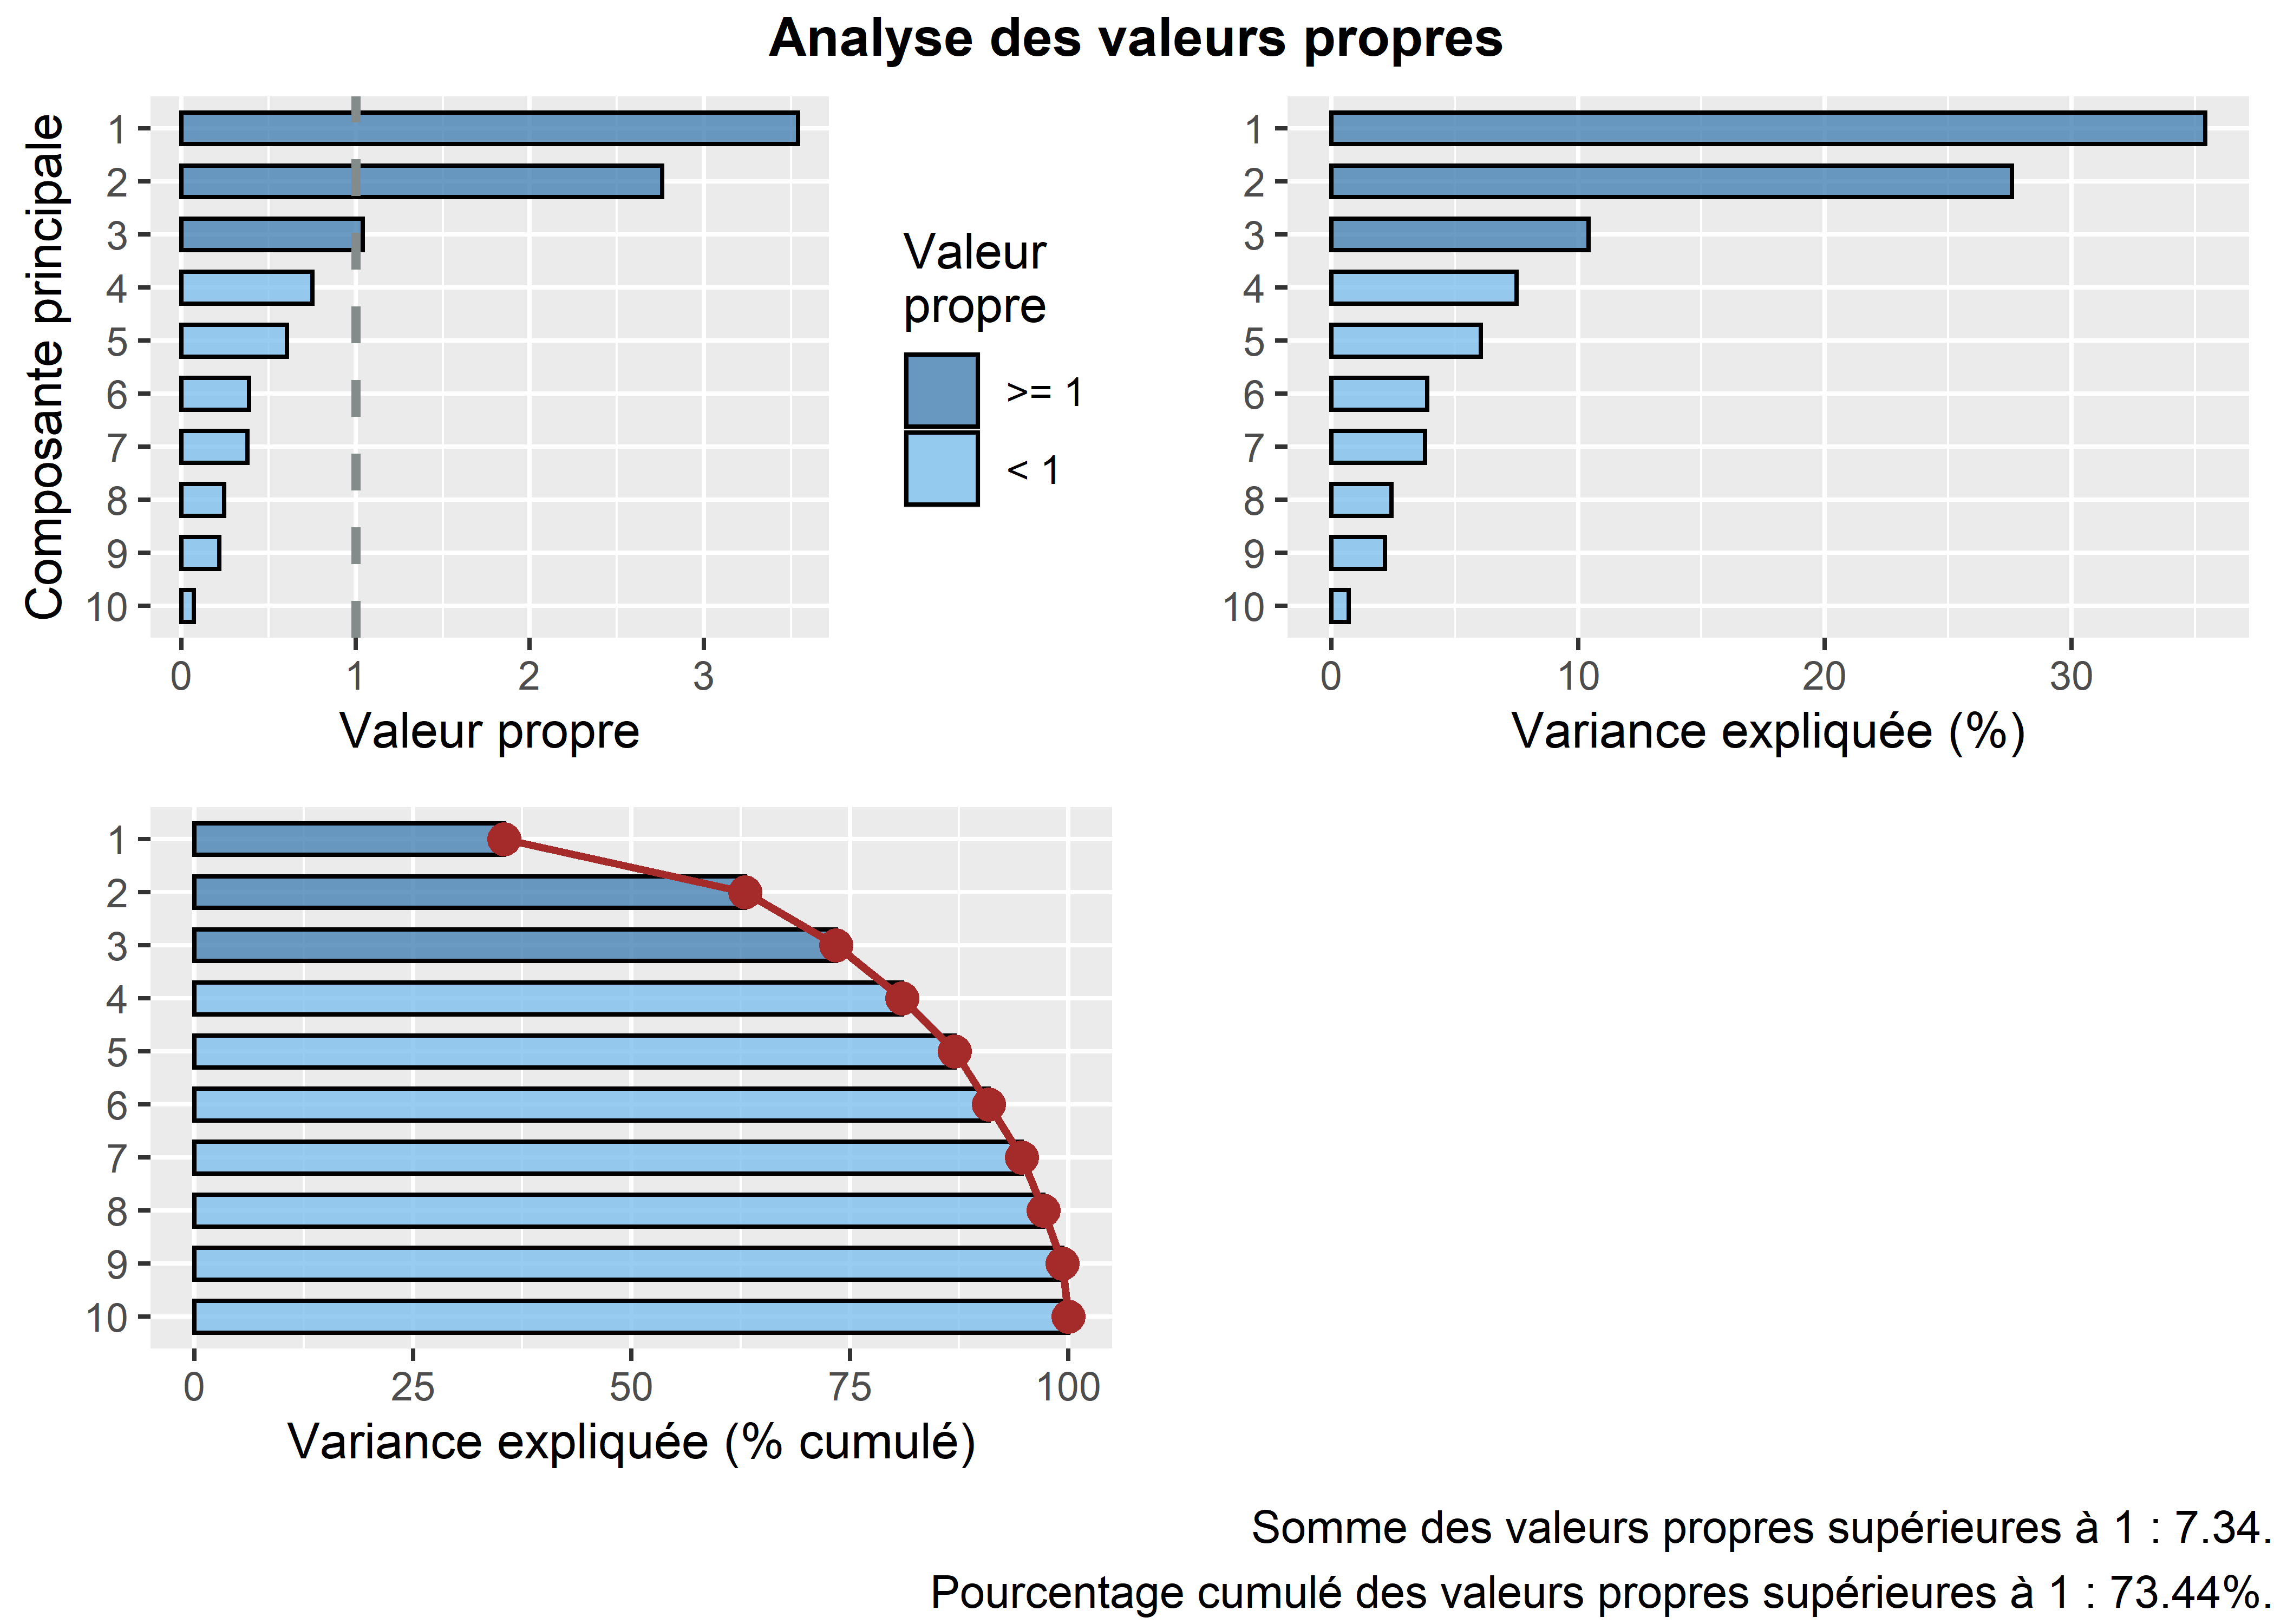
\includegraphics[width=0.75\linewidth]{livre_statistique_Phil_Jere_clean_files/figure-latex/acpmesgraphs1-1} 

}

\caption{Graphiques personnalisés pour les valeurs propres}\label{fig:acpmesgraphs1}
\end{figure}

Deuxièmement, la syntaxe ci-dessous permet de~:

\begin{itemize}
\tightlist
\item
  Construire un \emph{dataframe} avec les résultats des variables.
\item
  Construire des histogrammes avec les coordonnées des variables sur les axes factoriels (figure~\ref{fig:acpmesgraphs2}). Notez que les coordonnées négatives sont indiquées avec des barres bleues et celles négatives avec des barres de couleur saumon.
\item
  Un graphique avec les contributions des variables sur les axes retenus (figure~\ref{fig:acpmesgraphs3}).
\item
  Un graphique avec les cosinus carrés des variables sur les axes retenus (figure~\ref{fig:acpmesgraphs4}).
\item
  Un histogramme avec la qualité des variables sur les axes retenus (figure~\ref{fig:acpmesgraphs5}), soit la sommation de leurs cosinus carrés sur les axes retenus.
\end{itemize}

\begin{Shaded}
\begin{Highlighting}[]
\CommentTok{# Analyse des résultats de L'ACP pour les variables}
\KeywordTok{library}\NormalTok{(corrplot)}
\KeywordTok{library}\NormalTok{(stringr)}
\KeywordTok{library}\NormalTok{(ggplot2)}
\KeywordTok{library}\NormalTok{(ggpubr)}

\CommentTok{# Indiquer le nombre d'axes à conserver suite à l'analyse des valeurs propres}
\NormalTok{nComp <-}\StringTok{ }\DecValTok{3}
\CommentTok{# Variance expliquée par les axes retenus}
\NormalTok{vppct <-}\StringTok{ }\KeywordTok{round}\NormalTok{(dfACPvp[}\DecValTok{1}\OperatorTok{:}\NormalTok{nComp,}\StringTok{"VP_pct"}\NormalTok{],}\DecValTok{1}\NormalTok{)}
\CommentTok{# Dataframe des résultats pour les variables}
\NormalTok{CoordsVar <-}\StringTok{ }\NormalTok{res.acp}\OperatorTok{$}\NormalTok{var}\OperatorTok{$}\NormalTok{coord[, }\DecValTok{1}\OperatorTok{:}\NormalTok{nComp]}
\NormalTok{Cos2Var   <-}\StringTok{ }\NormalTok{res.acp}\OperatorTok{$}\NormalTok{var}\OperatorTok{$}\NormalTok{cos2[, }\DecValTok{1}\OperatorTok{:}\NormalTok{nComp]}
\NormalTok{CtrVar   <-}\StringTok{ }\NormalTok{res.acp}\OperatorTok{$}\NormalTok{var}\OperatorTok{$}\NormalTok{contrib[, }\DecValTok{1}\OperatorTok{:}\NormalTok{nComp]}
\NormalTok{dfACPVars <-}\StringTok{ }\KeywordTok{data.frame}\NormalTok{(}\DataTypeTok{Variable =}  \KeywordTok{row.names}\NormalTok{(res.acp}\OperatorTok{$}\NormalTok{var}\OperatorTok{$}\NormalTok{coord[, }\DecValTok{1}\OperatorTok{:}\NormalTok{nComp]),}
                        \DataTypeTok{Coord =}\NormalTok{ CoordsVar,}
                        \DataTypeTok{Cos2 =}\NormalTok{ Cos2Var,}
                        \DataTypeTok{Qualite =} \KeywordTok{rowSums}\NormalTok{(Cos2Var),}
                        \DataTypeTok{Ctr =}\NormalTok{ CtrVar)}
\KeywordTok{row.names}\NormalTok{(dfACPVars) <-}\StringTok{ }\OtherTok{NULL}
\KeywordTok{names}\NormalTok{(dfACPVars) <-}\StringTok{ }\KeywordTok{str_replace}\NormalTok{(}\KeywordTok{names}\NormalTok{(dfACPVars), }\StringTok{".Dim."}\NormalTok{, }\StringTok{"Comp"}\NormalTok{)}
\NormalTok{dfACPVars}

\CommentTok{# Histogrammes pour les coordonnées}
\NormalTok{couleursCoords <-}\StringTok{ }\KeywordTok{c}\NormalTok{(}\StringTok{"lightsalmon"}\NormalTok{,}\StringTok{"steelblue"}\NormalTok{)}
\NormalTok{plotCoordF1 <-}\StringTok{ }\KeywordTok{ggplot}\NormalTok{(dfACPVars,}
                      \KeywordTok{aes}\NormalTok{(}\DataTypeTok{y =} \KeywordTok{reorder}\NormalTok{(Variable, CoordComp1),}
                          \DataTypeTok{x =}\NormalTok{ CoordComp1, }\DataTypeTok{fill=}\NormalTok{CoordComp1}\OperatorTok{<}\DecValTok{0}\NormalTok{))}\OperatorTok{+}
\StringTok{  }\KeywordTok{geom_bar}\NormalTok{(}\DataTypeTok{stat=}\StringTok{"identity"}\NormalTok{, }\DataTypeTok{width =} \FloatTok{.6}\NormalTok{, }\DataTypeTok{alpha=}\NormalTok{.}\DecValTok{8}\NormalTok{, }\DataTypeTok{color=}\StringTok{"black"}\NormalTok{)}\OperatorTok{+}
\StringTok{  }\KeywordTok{geom_vline}\NormalTok{(}\DataTypeTok{xintercept=}\DecValTok{0}\NormalTok{, }\DataTypeTok{color =} \StringTok{"black"}\NormalTok{, }\DataTypeTok{size=}\DecValTok{1}\NormalTok{)}\OperatorTok{+}
\StringTok{  }\KeywordTok{scale_fill_manual}\NormalTok{(}\DataTypeTok{name=}\StringTok{"Coordonnée"}\NormalTok{,}\DataTypeTok{values=}\NormalTok{couleursCoords,}
                    \DataTypeTok{labels =} \KeywordTok{c}\NormalTok{(}\StringTok{"Positive"}\NormalTok{,}\StringTok{"Négative"}\NormalTok{))}\OperatorTok{+}
\StringTok{  }\KeywordTok{labs}\NormalTok{(}\DataTypeTok{x=}\KeywordTok{paste0}\NormalTok{(}\StringTok{"Axe 1 ("}\NormalTok{, vppct[}\DecValTok{1}\NormalTok{],}\StringTok{"%)"}\NormalTok{), }\DataTypeTok{y=}\StringTok{"Variable"}\NormalTok{)}\OperatorTok{+}
\StringTok{  }\KeywordTok{theme}\NormalTok{(}\DataTypeTok{legend.position=}\StringTok{"none"}\NormalTok{)}
\NormalTok{plotCoordF2 <-}\StringTok{ }\KeywordTok{ggplot}\NormalTok{(dfACPVars,}
                      \KeywordTok{aes}\NormalTok{(}\DataTypeTok{y =} \KeywordTok{reorder}\NormalTok{(Variable, CoordComp2),}
                          \DataTypeTok{x =}\NormalTok{ CoordComp2, }\DataTypeTok{fill=}\NormalTok{CoordComp2}\OperatorTok{<}\DecValTok{0}\NormalTok{))}\OperatorTok{+}
\StringTok{  }\KeywordTok{geom_bar}\NormalTok{(}\DataTypeTok{stat=}\StringTok{"identity"}\NormalTok{, }\DataTypeTok{width =} \FloatTok{.6}\NormalTok{, }\DataTypeTok{alpha=}\NormalTok{.}\DecValTok{8}\NormalTok{, }\DataTypeTok{color=}\StringTok{"black"}\NormalTok{)}\OperatorTok{+}
\StringTok{  }\KeywordTok{geom_vline}\NormalTok{(}\DataTypeTok{xintercept=}\DecValTok{0}\NormalTok{, }\DataTypeTok{color =} \StringTok{"black"}\NormalTok{, }\DataTypeTok{size=}\DecValTok{1}\NormalTok{)}\OperatorTok{+}
\StringTok{  }\KeywordTok{scale_fill_manual}\NormalTok{(}\DataTypeTok{name=}\StringTok{"Coordonnée"}\NormalTok{,}\DataTypeTok{values=}\NormalTok{couleursCoords,}
                    \DataTypeTok{labels =} \KeywordTok{c}\NormalTok{(}\StringTok{"Positive"}\NormalTok{,}\StringTok{"Négative"}\NormalTok{))}\OperatorTok{+}
\StringTok{  }\KeywordTok{labs}\NormalTok{(}\DataTypeTok{x=}\KeywordTok{paste0}\NormalTok{(}\StringTok{"Axe 2 ("}\NormalTok{, vppct[}\DecValTok{2}\NormalTok{],}\StringTok{"%)"}\NormalTok{), }\DataTypeTok{y=}\StringTok{"Variable"}\NormalTok{)}\OperatorTok{+}
\StringTok{  }\KeywordTok{theme}\NormalTok{(}\DataTypeTok{legend.position=}\StringTok{"none"}\NormalTok{)}
\NormalTok{plotCoordF3 <-}\StringTok{ }\KeywordTok{ggplot}\NormalTok{(dfACPVars,}
                      \KeywordTok{aes}\NormalTok{(}\DataTypeTok{y =} \KeywordTok{reorder}\NormalTok{(Variable, CoordComp3),}
                          \DataTypeTok{x =}\NormalTok{ CoordComp3, }\DataTypeTok{fill=}\NormalTok{CoordComp3}\OperatorTok{<}\DecValTok{0}\NormalTok{))}\OperatorTok{+}
\StringTok{  }\KeywordTok{geom_bar}\NormalTok{(}\DataTypeTok{stat=}\StringTok{"identity"}\NormalTok{, }\DataTypeTok{width =} \FloatTok{.6}\NormalTok{, }\DataTypeTok{alpha=}\NormalTok{.}\DecValTok{8}\NormalTok{, }\DataTypeTok{color=}\StringTok{"black"}\NormalTok{)}\OperatorTok{+}
\StringTok{  }\KeywordTok{geom_vline}\NormalTok{(}\DataTypeTok{xintercept=}\DecValTok{0}\NormalTok{, }\DataTypeTok{color =} \StringTok{"black"}\NormalTok{, }\DataTypeTok{size=}\DecValTok{1}\NormalTok{)}\OperatorTok{+}
\StringTok{  }\KeywordTok{scale_fill_manual}\NormalTok{(}\DataTypeTok{name=}\StringTok{"Coordonnée"}\NormalTok{, }\DataTypeTok{values=}\NormalTok{couleursCoords,}
                    \DataTypeTok{labels =} \KeywordTok{c}\NormalTok{(}\StringTok{"Positive"}\NormalTok{,}\StringTok{"Négative"}\NormalTok{))}\OperatorTok{+}
\StringTok{  }\KeywordTok{labs}\NormalTok{(}\DataTypeTok{x=}\KeywordTok{paste0}\NormalTok{(}\StringTok{"Axe 3 ("}\NormalTok{, vppct[}\DecValTok{3}\NormalTok{],}\StringTok{"%)"}\NormalTok{), }\DataTypeTok{y=}\StringTok{"Variable"}\NormalTok{)}

\KeywordTok{annotate_figure}\NormalTok{(}\KeywordTok{ggarrange}\NormalTok{(plotCoordF1, plotCoordF2, plotCoordF3, }\DataTypeTok{nrow=}\NormalTok{nComp),}
                \KeywordTok{text_grob}\NormalTok{(}\StringTok{"Coordonnées des variables sur les axes factoriels"}\NormalTok{,}
                          \DataTypeTok{color =} \StringTok{"black"}\NormalTok{, }\DataTypeTok{face =} \StringTok{"bold"}\NormalTok{, }\DataTypeTok{size =} \DecValTok{12}\NormalTok{))}

\CommentTok{# Contributions des variables à la formation des axes}
\NormalTok{couleurs <-}\StringTok{ }\KeywordTok{colorRampPalette}\NormalTok{(}\KeywordTok{c}\NormalTok{(}\StringTok{"#ffffd4"}\NormalTok{,}\StringTok{"#993404"}\NormalTok{))}
\KeywordTok{corrplot}\NormalTok{(CtrVar, }\DataTypeTok{is.corr=}\OtherTok{FALSE}\NormalTok{, }\DataTypeTok{method =}\StringTok{"square"}\NormalTok{, }\DataTypeTok{col =} \KeywordTok{couleurs}\NormalTok{(}\DecValTok{20}\NormalTok{),}
         \DataTypeTok{addCoef.col =} \DecValTok{1}\NormalTok{, }\DataTypeTok{cl.pos =} \OtherTok{FALSE}\NormalTok{)}

\CommentTok{# La qualité des variables sur les composantes retenues : cosinus carrés}
\KeywordTok{corrplot}\NormalTok{(Cos2Var, }\DataTypeTok{is.corr=}\OtherTok{FALSE}\NormalTok{, }\DataTypeTok{method =}\StringTok{"square"}\NormalTok{, }\DataTypeTok{col =} \KeywordTok{couleurs}\NormalTok{(}\DecValTok{20}\NormalTok{),}
         \DataTypeTok{addCoef.col =} \DecValTok{1}\NormalTok{, }\DataTypeTok{cl.pos =} \OtherTok{FALSE}\NormalTok{)}

\KeywordTok{ggplot}\NormalTok{(dfACPVars)}\OperatorTok{+}
\StringTok{  }\KeywordTok{geom_bar}\NormalTok{(}\KeywordTok{aes}\NormalTok{(}\DataTypeTok{y=}\KeywordTok{reorder}\NormalTok{(Variable, Qualite), }\DataTypeTok{x=}\NormalTok{Qualite),}
            \DataTypeTok{stat=}\StringTok{"identity"}\NormalTok{, }\DataTypeTok{width =} \FloatTok{.6}\NormalTok{, }\DataTypeTok{alpha=}\NormalTok{.}\DecValTok{8}\NormalTok{, }\DataTypeTok{fill=}\StringTok{"steelblue"}\NormalTok{)}\OperatorTok{+}
\StringTok{  }\KeywordTok{labs}\NormalTok{(}\DataTypeTok{x=}\StringTok{""}\NormalTok{, }\DataTypeTok{y=}\StringTok{"Somme des cosinus carrés sur les axes retenus"}\NormalTok{,}
       \DataTypeTok{title =}\StringTok{"Qualité de représentation des variables sur les axes retenus de l'ACP"}\NormalTok{,}
       \DataTypeTok{subtitle =} \KeywordTok{paste0}\NormalTok{(}\StringTok{"Variance expliquée par les "}\NormalTok{, nComp, }
                         \StringTok{" composantes : "}\NormalTok{, }\KeywordTok{sum}\NormalTok{(vppct), }\StringTok{"%"}\NormalTok{))}
\end{Highlighting}
\end{Shaded}

\begin{figure}

{\centering 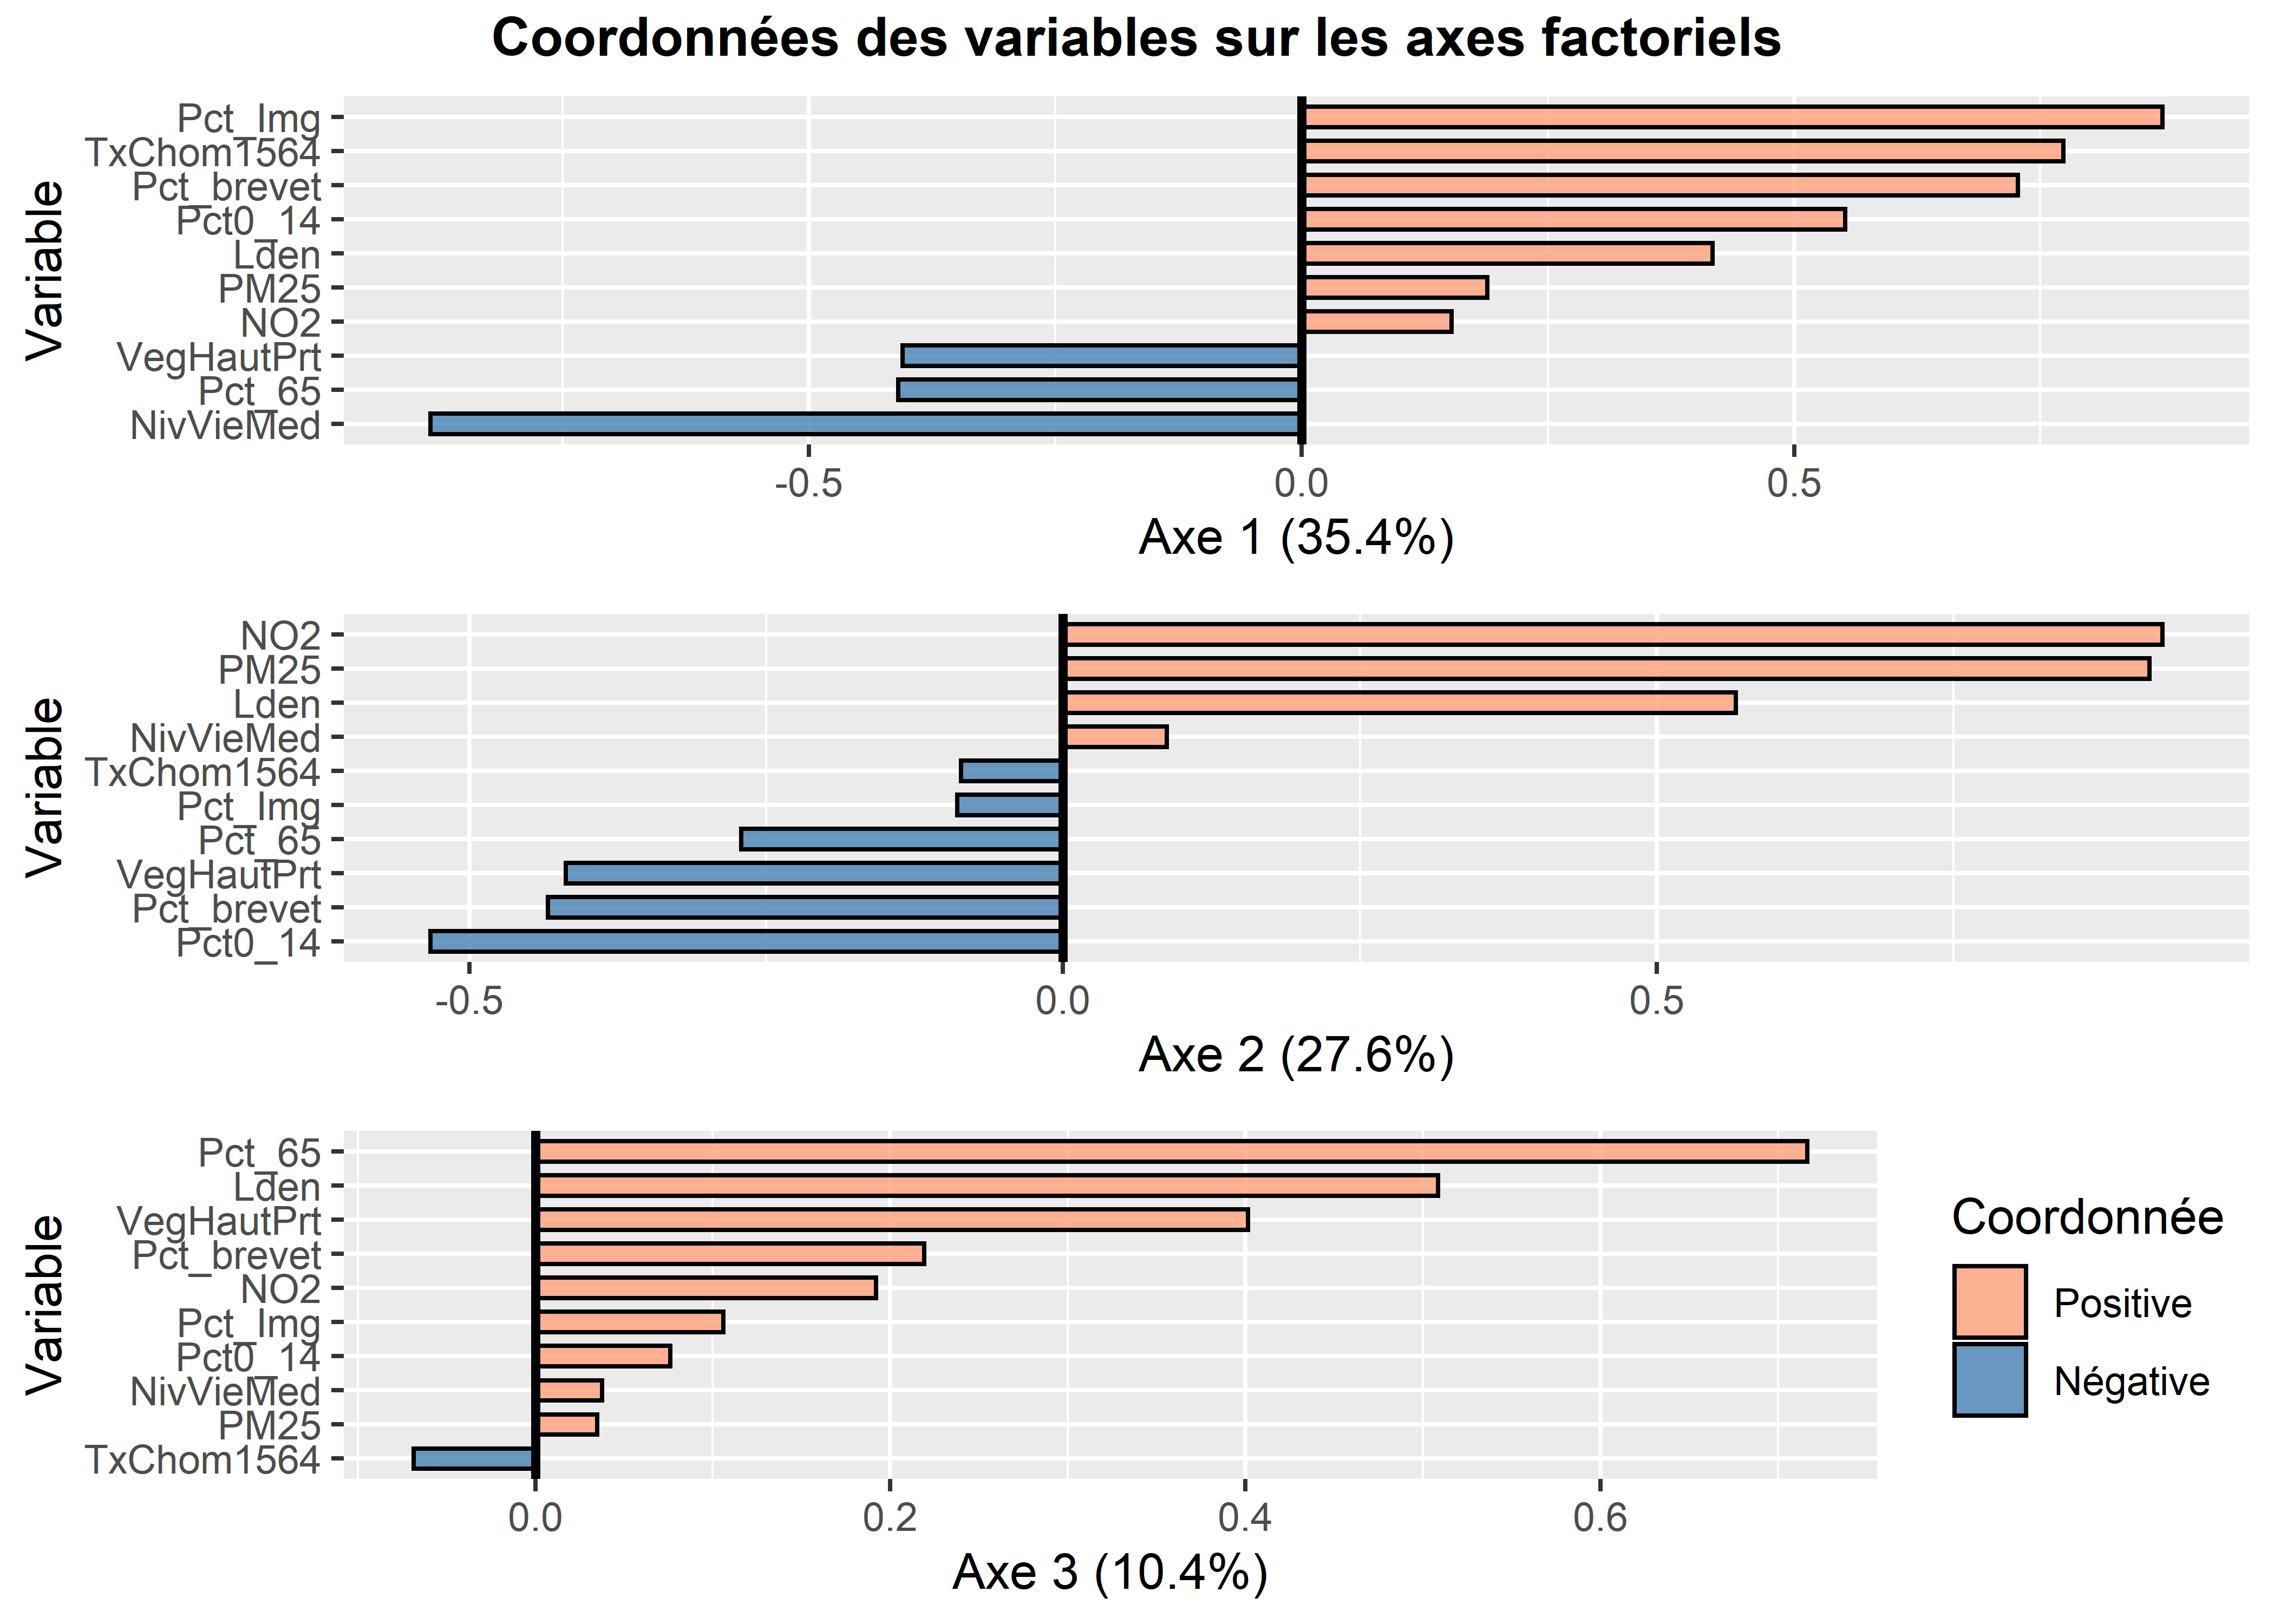
\includegraphics[width=0.75\linewidth]{livre_statistique_Phil_Jere_clean_files/figure-latex/acpmesgraphs2-1} 

}

\caption{Histogrammes personnalisés avec les coordonnées factorielles pour les variables}\label{fig:acpmesgraphs2}
\end{figure}

\begin{figure}

{\centering 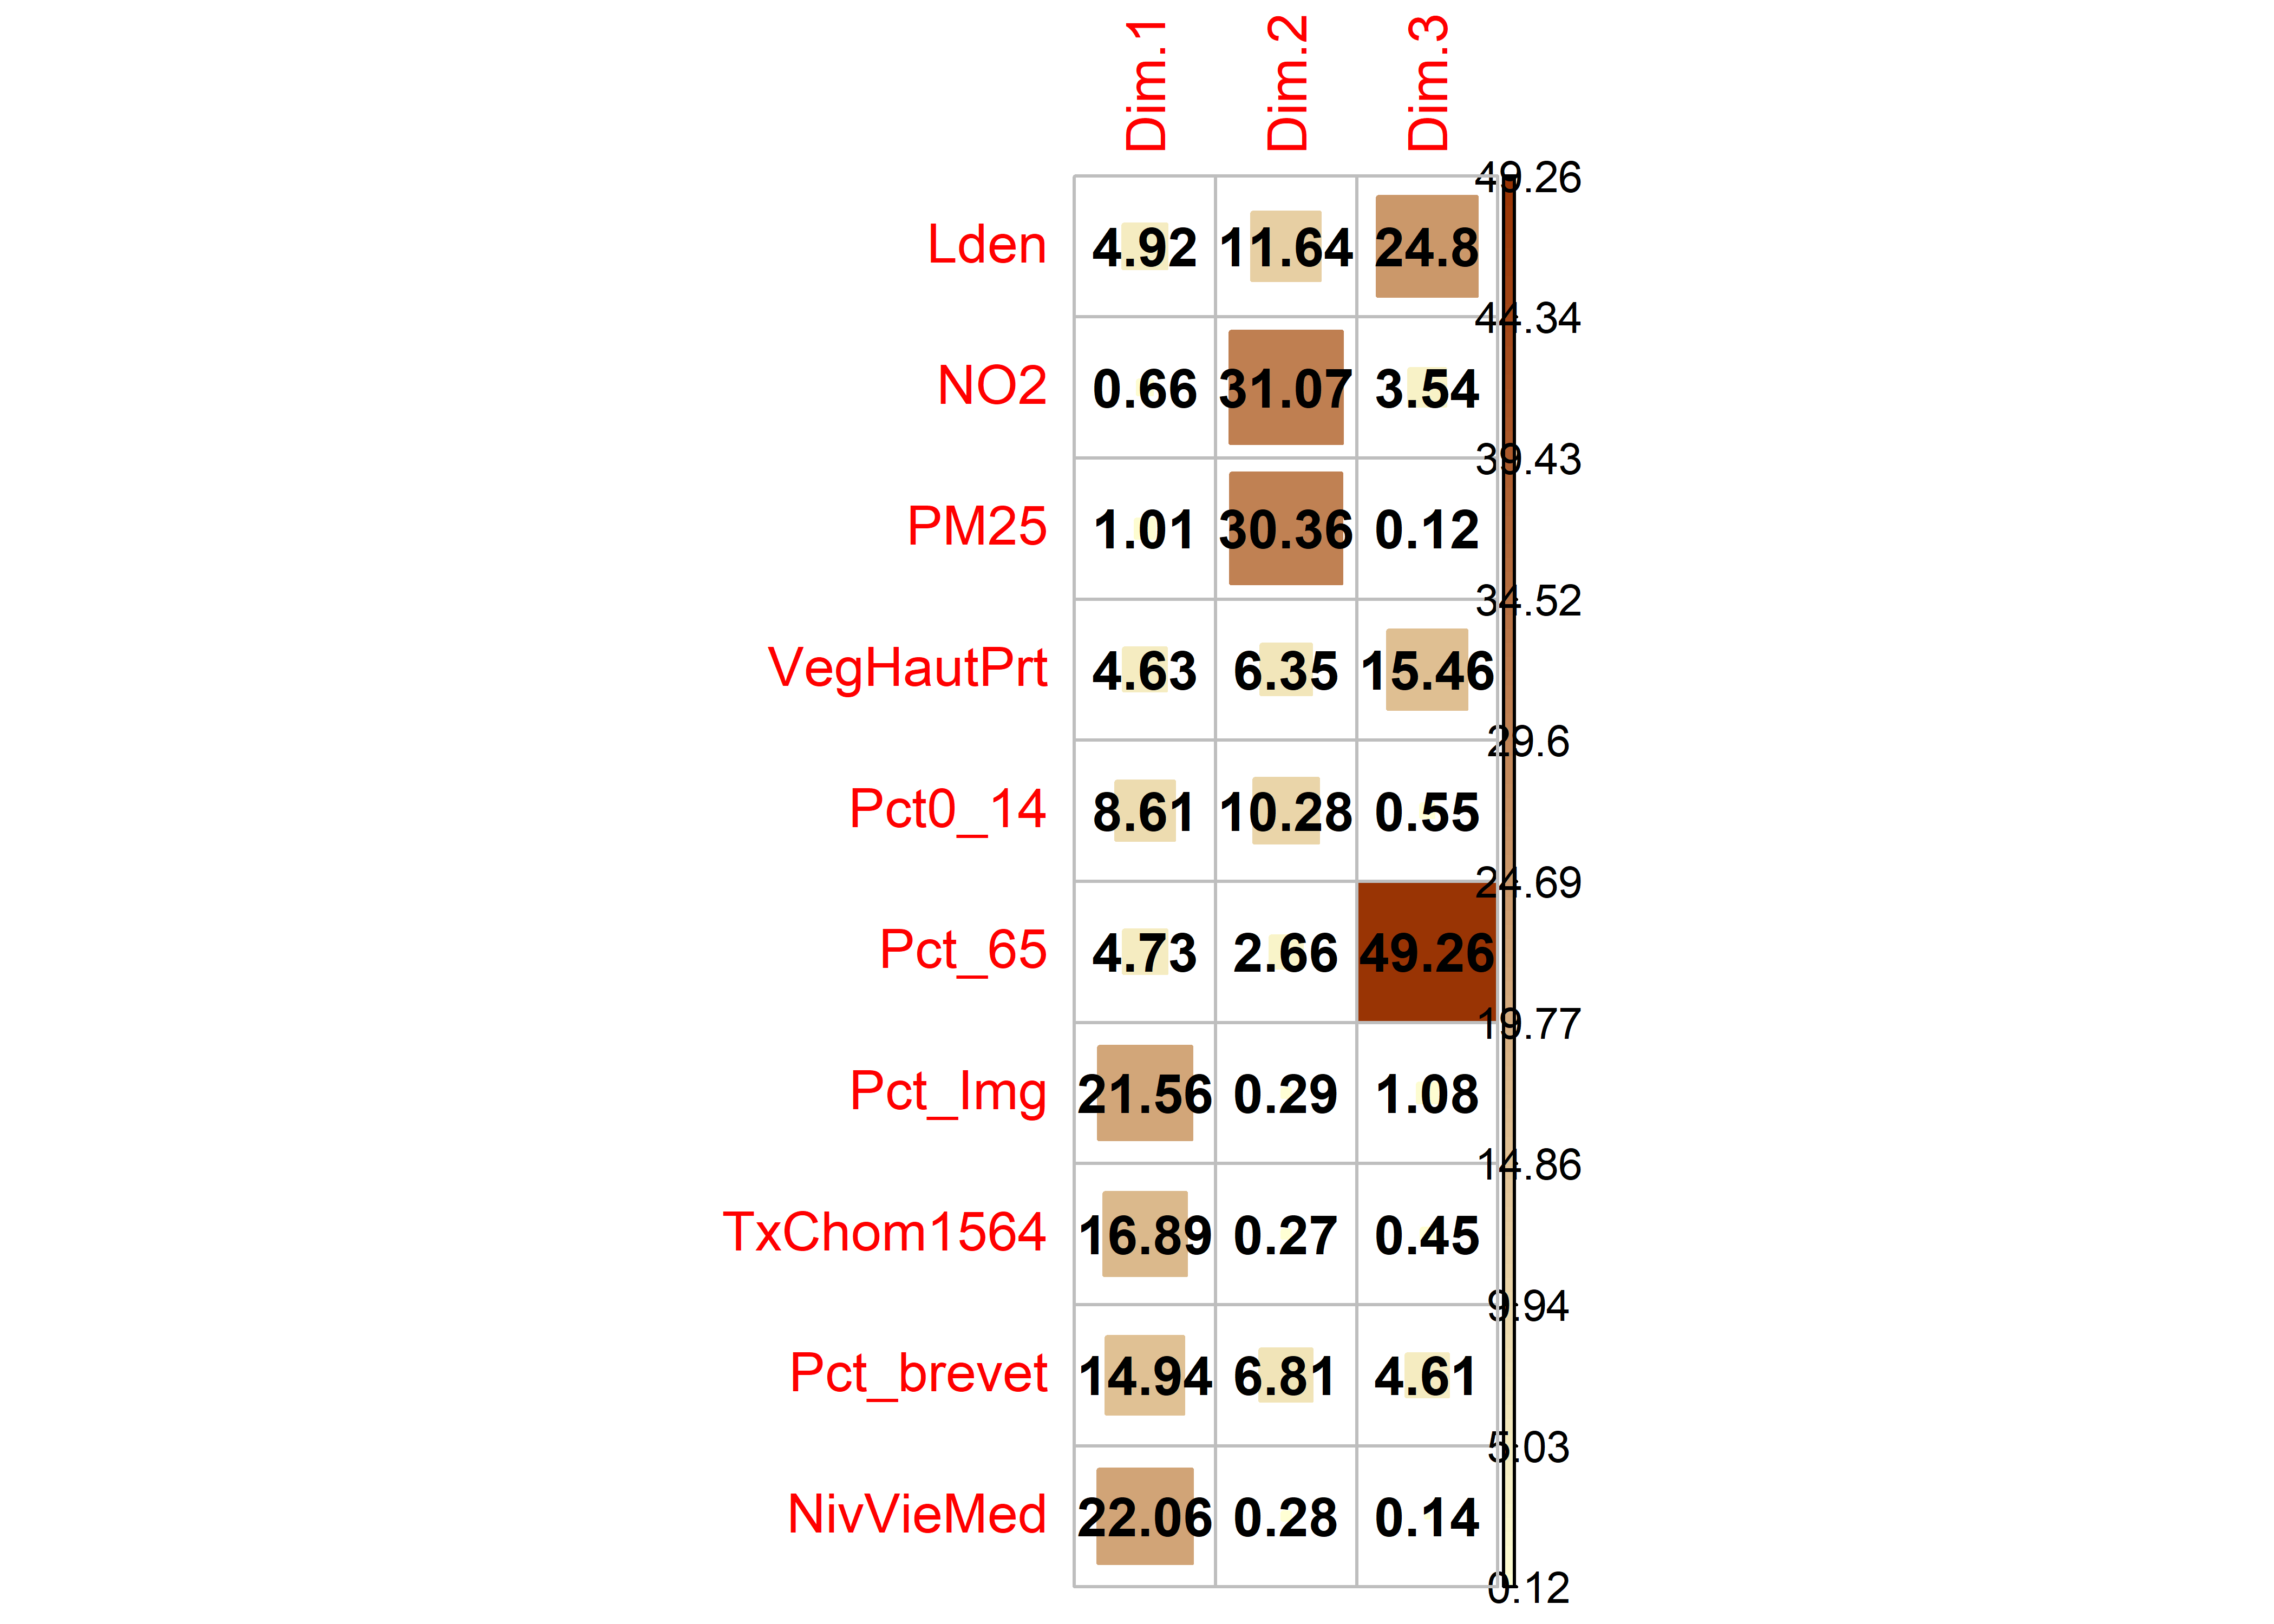
\includegraphics[width=0.75\linewidth]{livre_statistique_Phil_Jere_clean_files/figure-latex/acpmesgraphs3-1} 

}

\caption{Graphiques personnalisés avec les contributions des variables}\label{fig:acpmesgraphs3}
\end{figure}

\begin{figure}

{\centering 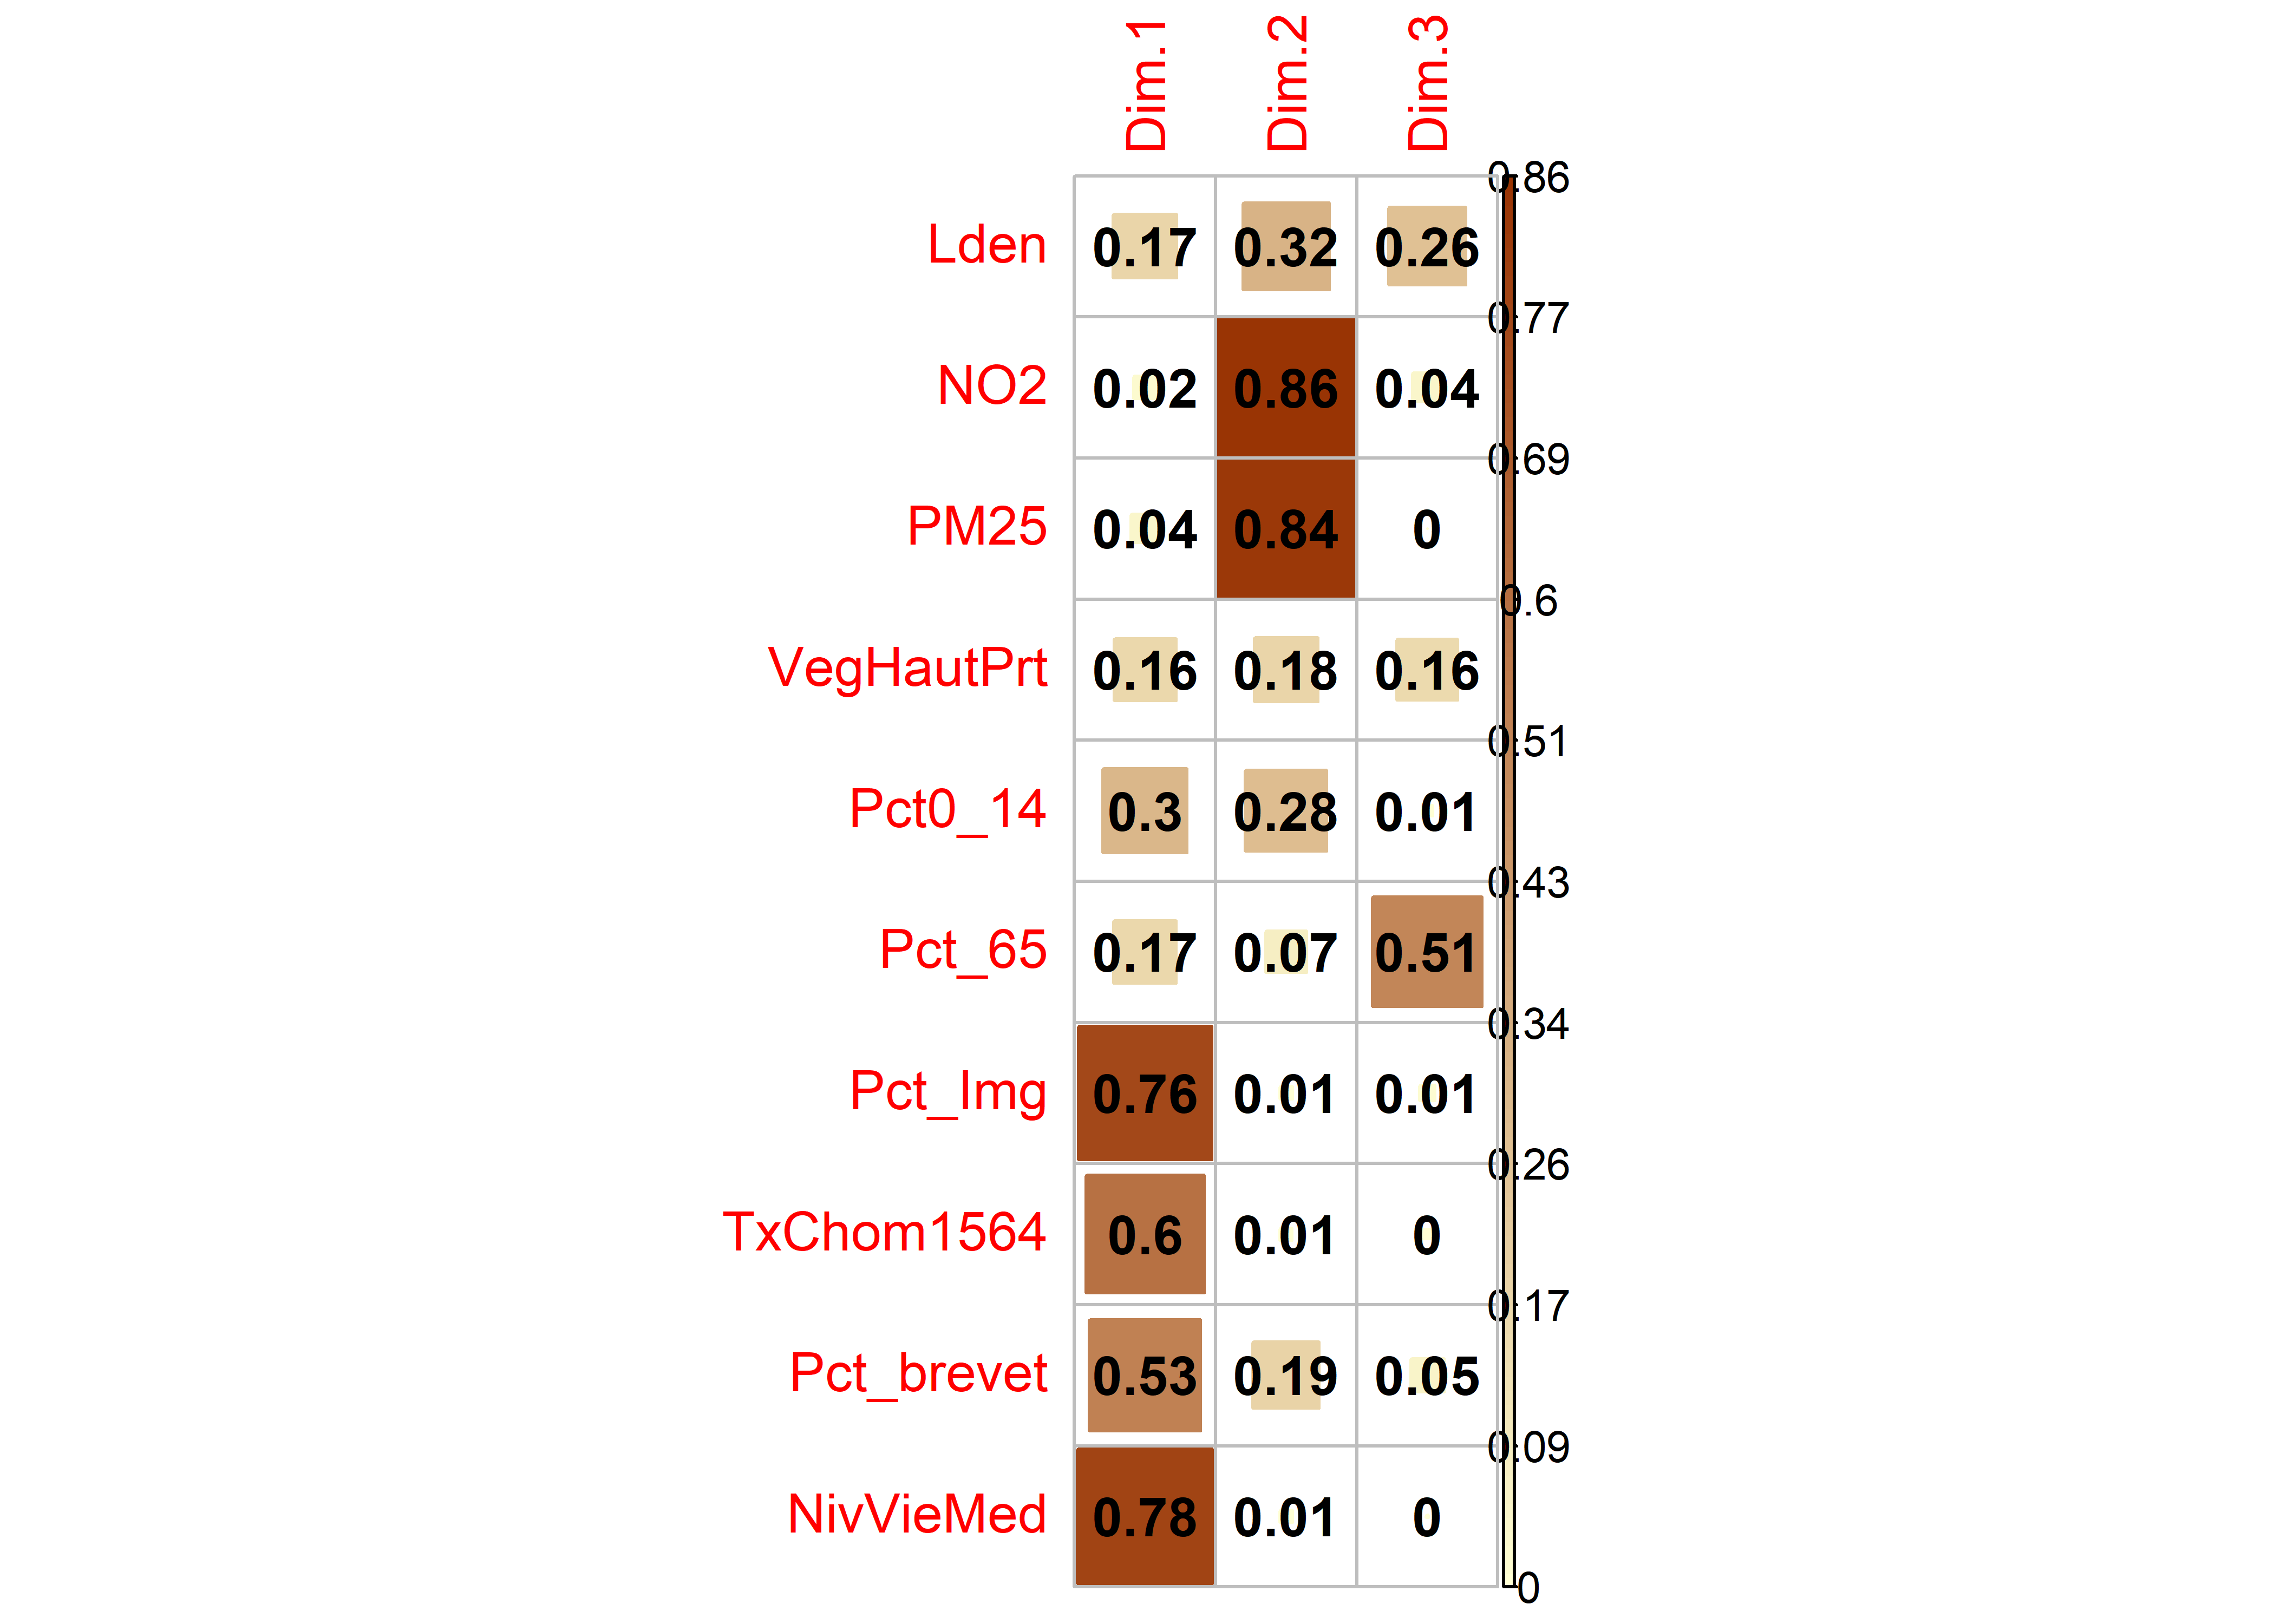
\includegraphics[width=0.75\linewidth]{livre_statistique_Phil_Jere_clean_files/figure-latex/acpmesgraphs4-1} 

}

\caption{Graphiques personnalisés avec les cosinus carrés des variables}\label{fig:acpmesgraphs4}
\end{figure}

\begin{figure}

{\centering 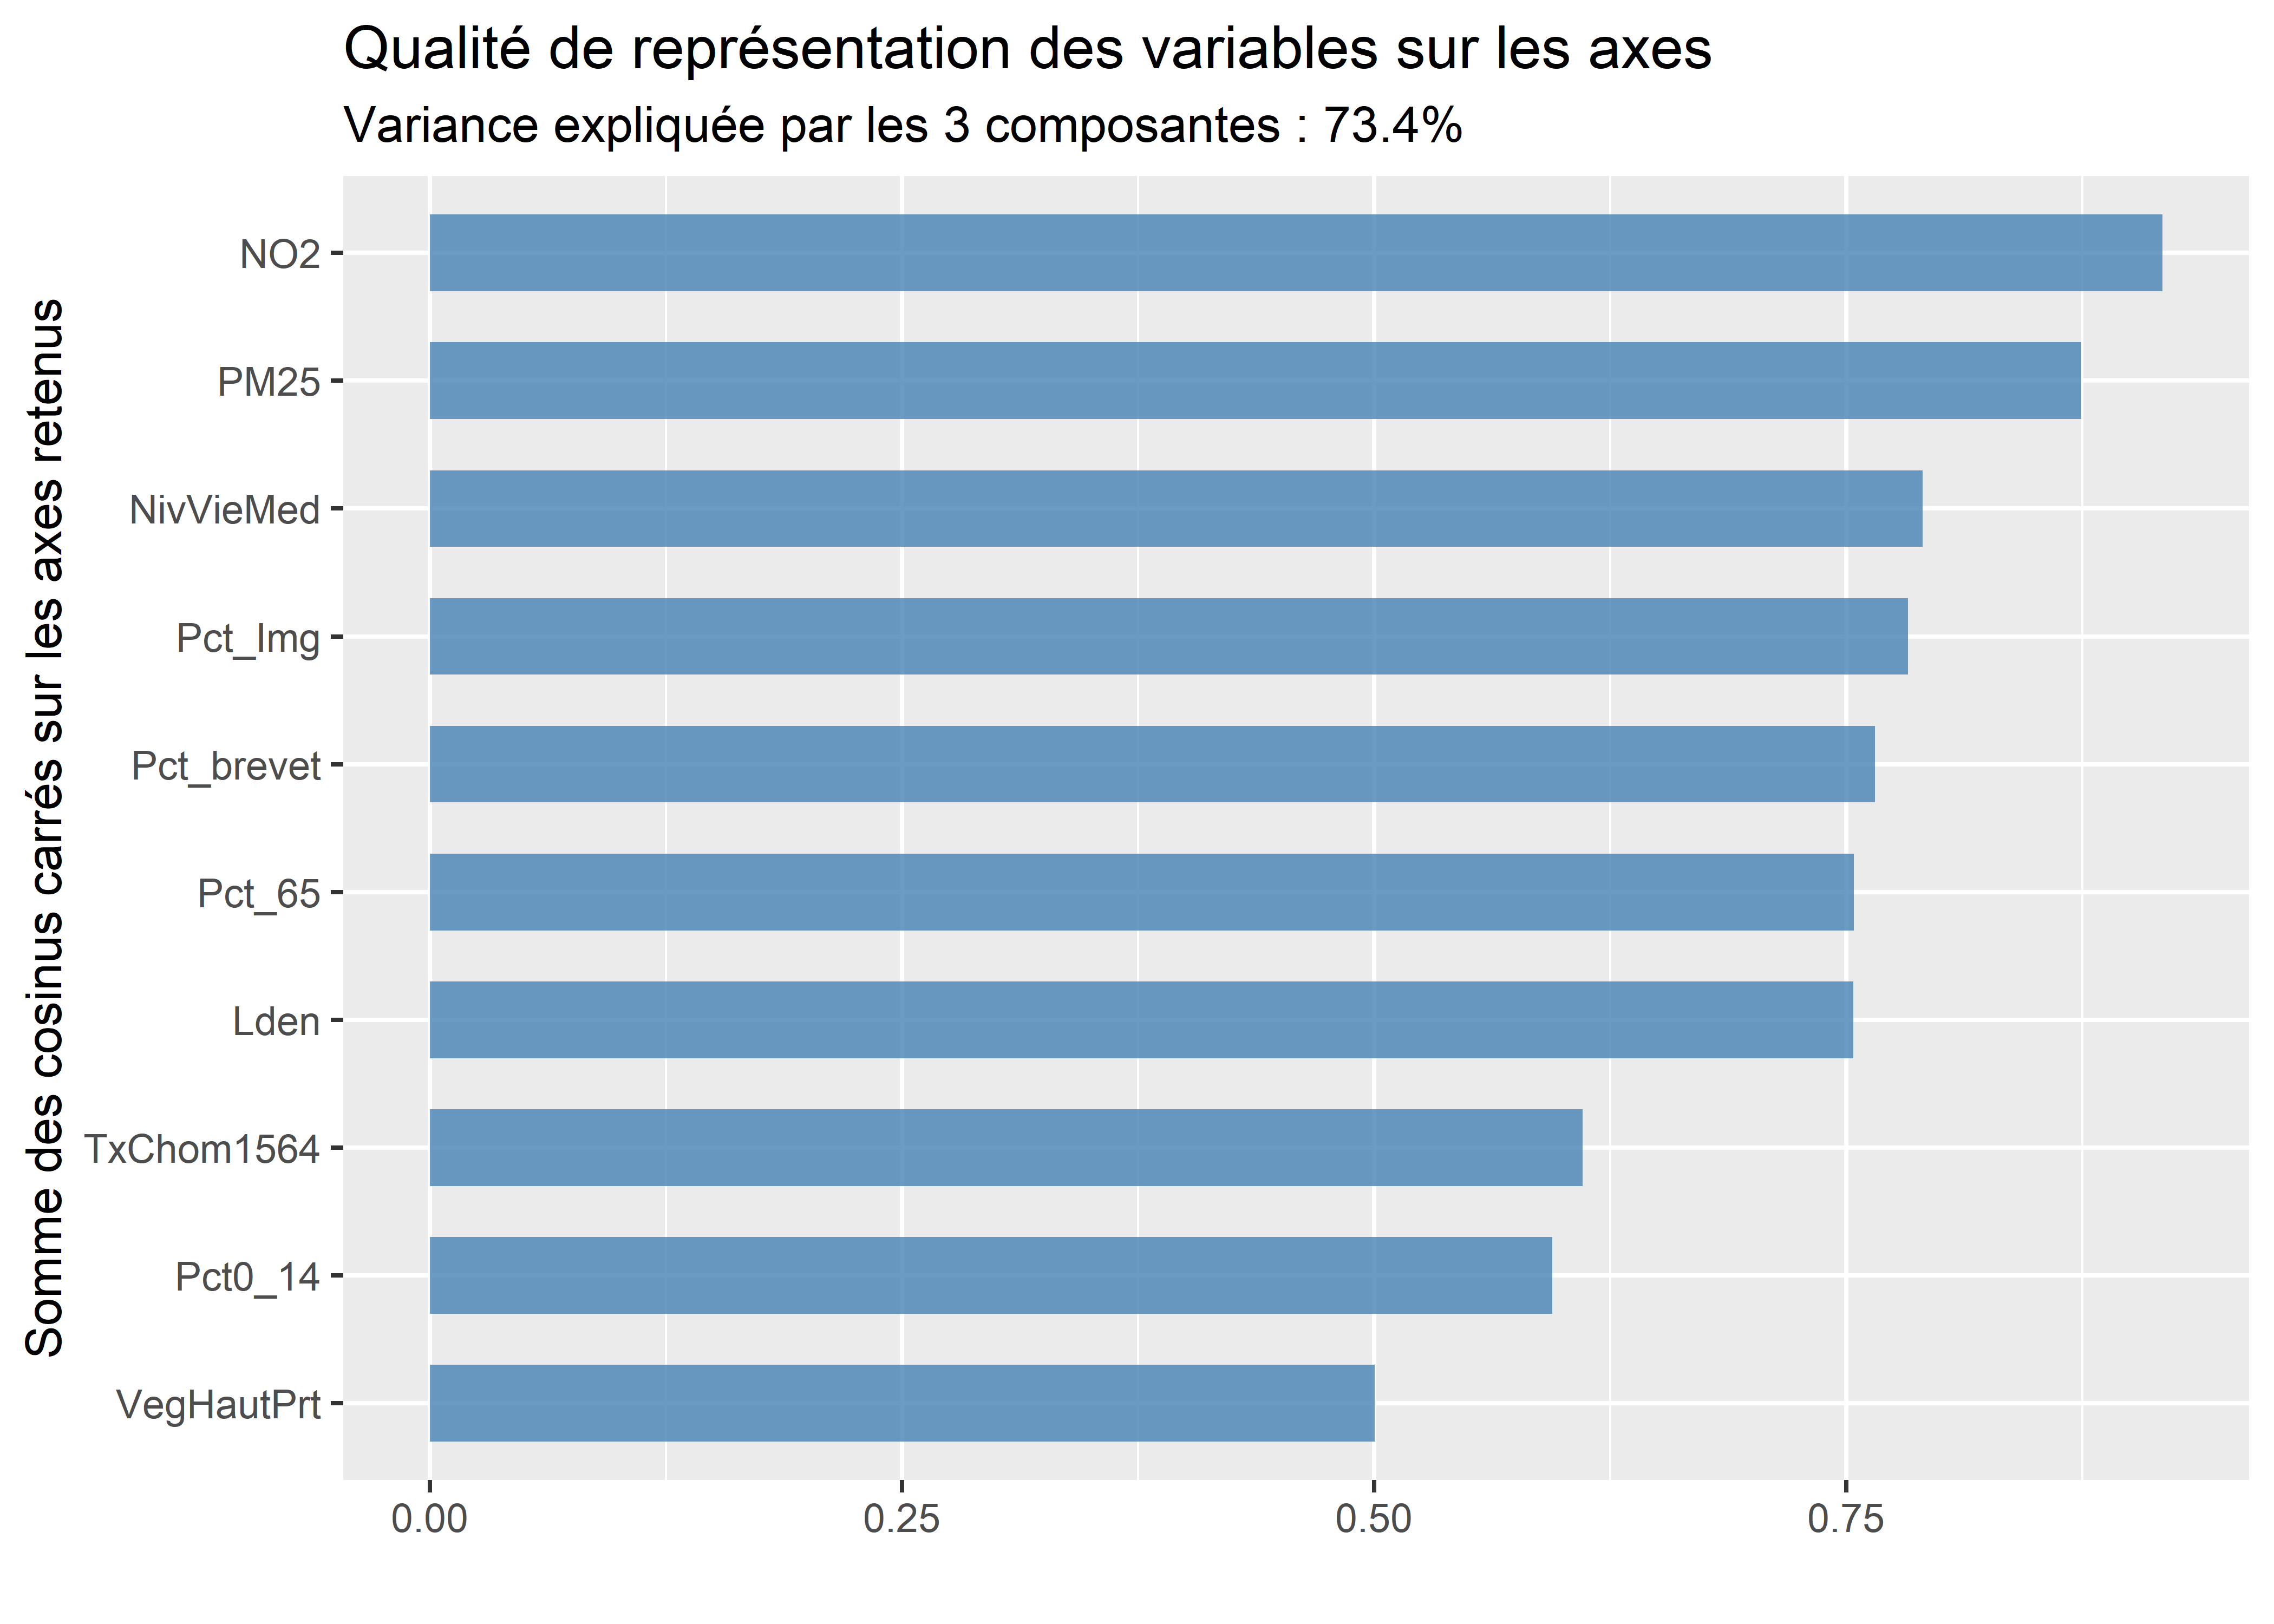
\includegraphics[width=0.75\linewidth]{livre_statistique_Phil_Jere_clean_files/figure-latex/acpmesgraphs5-1} 

}

\caption{Graphique personnalisé avec la qualité des variables sur les axes retenus de l'ACP}\label{fig:acpmesgraphs5}
\end{figure}

Troisièmement, lorsque les observations sont des unités spatiales, il convient de cartographier les coordonnées factorielles des individus. Dans le jeu de données utilisé, les observations sont des polygones délimitant les îlots regroupés pour l'information statistique (IRIS) pour l'agglomération de Lyon (France). Nous utilisons les \emph{packages} \texttt{tmap} et \texttt{RColorBrewer} pour réaliser des cartes choroplèthes avec les coordonnées deux premières composantes (figure~\ref{fig:acpmesgraphs6}).

\begin{Shaded}
\begin{Highlighting}[]
\KeywordTok{library}\NormalTok{(}\StringTok{"tmap"}\NormalTok{)}
\KeywordTok{library}\NormalTok{(}\StringTok{"RColorBrewer"}\NormalTok{)}
\CommentTok{# Analyse des résultats de l'ACP pour les individus}
\CommentTok{# Dataframe des résultats pour les individus}
\NormalTok{CoordsInd <-}\StringTok{ }\NormalTok{res.acp}\OperatorTok{$}\NormalTok{ind}\OperatorTok{$}\NormalTok{coord[, }\DecValTok{1}\OperatorTok{:}\NormalTok{nComp]}
\NormalTok{Cos2Ind   <-}\StringTok{ }\NormalTok{res.acp}\OperatorTok{$}\NormalTok{ind}\OperatorTok{$}\NormalTok{cos2[, }\DecValTok{1}\OperatorTok{:}\NormalTok{nComp]}
\NormalTok{CtrInd    <-}\StringTok{ }\NormalTok{res.acp}\OperatorTok{$}\NormalTok{ind}\OperatorTok{$}\NormalTok{contrib[, }\DecValTok{1}\OperatorTok{:}\NormalTok{nComp]}
\NormalTok{dfACPInd <-}\StringTok{ }\KeywordTok{data.frame}\NormalTok{(}\DataTypeTok{Coord =}\NormalTok{ CoordsInd, }\DataTypeTok{Cos2 =}\NormalTok{ Cos2Ind, }\DataTypeTok{Ctr =}\NormalTok{ CtrInd)}
\KeywordTok{names}\NormalTok{(dfACPInd) <-}\StringTok{ }\KeywordTok{str_replace}\NormalTok{(}\KeywordTok{names}\NormalTok{(dfACPInd), }\StringTok{".Dim."}\NormalTok{, }\StringTok{"Comp"}\NormalTok{)}
\CommentTok{# Fusion du tableau original avec les résultats de l'ACP pour les individus}
\NormalTok{CartoACP <-}\StringTok{ }\KeywordTok{cbind}\NormalTok{(LyonIris, dfACPInd)}
\CommentTok{# Cartographie des coordonnées factorielles pour les individus pour les}
\CommentTok{# deux premières composantes}
\NormalTok{Carte1 <-}\StringTok{ }\KeywordTok{tm_shape}\NormalTok{(CartoACP) }\OperatorTok{+}
\StringTok{          }\KeywordTok{tm_polygons}\NormalTok{(}\DataTypeTok{col =} \StringTok{"CoordComp1"}\NormalTok{, }\DataTypeTok{style =} \StringTok{"cont"}\NormalTok{,}
                      \DataTypeTok{midpoint =} \DecValTok{0}\NormalTok{, }\DataTypeTok{title =} \StringTok{'Coordonnées'}\NormalTok{)}\OperatorTok{+}
\StringTok{          }\KeywordTok{tm_layout}\NormalTok{(}\DataTypeTok{main.title =} \KeywordTok{paste0}\NormalTok{(}\StringTok{"Axe 1 ("}\NormalTok{, vppct[}\DecValTok{1}\NormalTok{],}\StringTok{"%)"}\NormalTok{),}
             \DataTypeTok{attr.outside =} \OtherTok{TRUE}\NormalTok{, }\DataTypeTok{frame =} \OtherTok{FALSE}\NormalTok{, }\DataTypeTok{main.title.size =} \DecValTok{1}\NormalTok{)}
\NormalTok{Carte2 <-}\StringTok{ }\KeywordTok{tm_shape}\NormalTok{(CartoACP) }\OperatorTok{+}
\StringTok{          }\KeywordTok{tm_polygons}\NormalTok{(}\DataTypeTok{col =} \StringTok{"CoordComp2"}\NormalTok{, }\DataTypeTok{style =} \StringTok{"cont"}\NormalTok{,}
                      \DataTypeTok{midpoint =} \DecValTok{0}\NormalTok{, }\DataTypeTok{title =} \StringTok{'Coordonnées'}\NormalTok{)}\OperatorTok{+}
\StringTok{  }\KeywordTok{tm_layout}\NormalTok{(}\DataTypeTok{main.title =} \KeywordTok{paste0}\NormalTok{(}\StringTok{"Axe 2 ("}\NormalTok{, vppct[}\DecValTok{2}\NormalTok{],}\StringTok{"%)"}\NormalTok{),}
             \DataTypeTok{attr.outside =} \OtherTok{TRUE}\NormalTok{, }\DataTypeTok{frame =} \OtherTok{FALSE}\NormalTok{, }\DataTypeTok{main.title.size =} \DecValTok{1}\NormalTok{)}
\KeywordTok{tmap_arrange}\NormalTok{(Carte1, Carte2)}
\end{Highlighting}
\end{Shaded}

\begin{figure}

{\centering 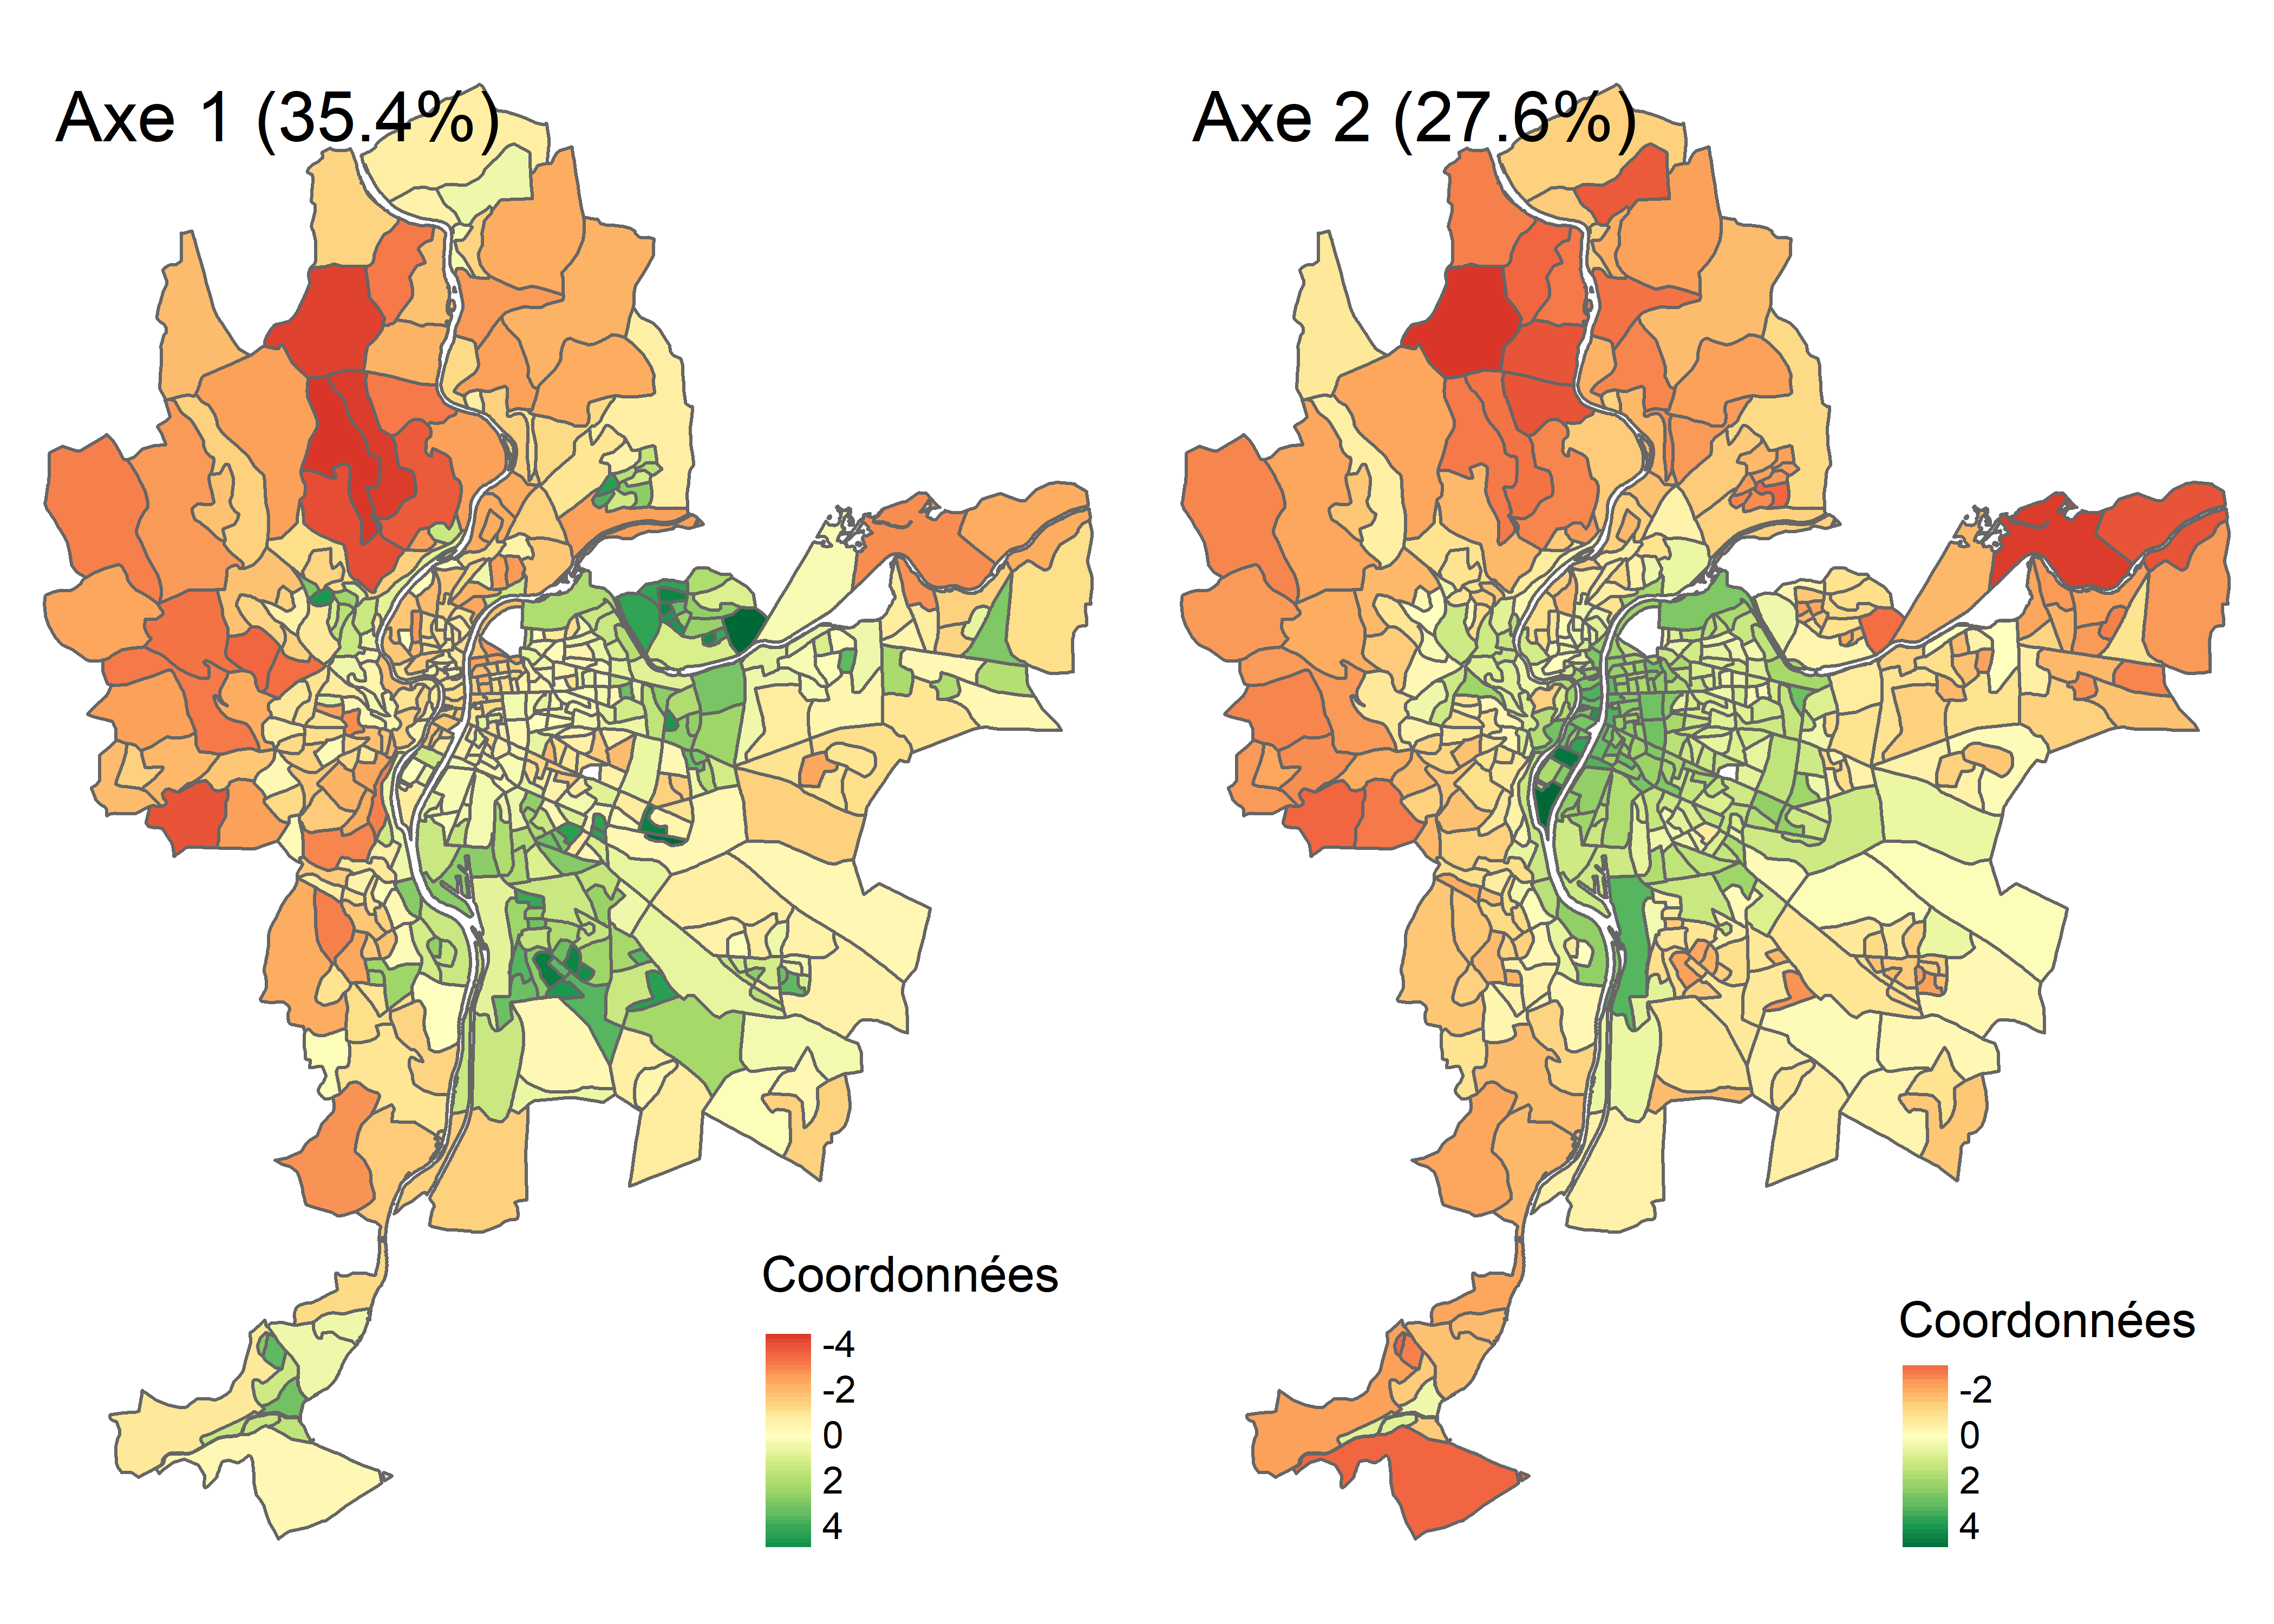
\includegraphics[width=0.75\linewidth]{livre_statistique_Phil_Jere_clean_files/figure-latex/acpmesgraphs6-1} 

}

\caption{Cartographie des coordonnées factorielles des individus}\label{fig:acpmesgraphs6}
\end{figure}

\begin{bloc_aller_loin}
\textbf{Exploration interactive des résultats d'une ACP avec le \emph{package} \texttt{explor}}.

Vous avez compris qu'il ne suffit pas de calculer une ACP, il faut retenir les \emph{n} premiers axes de l'ACP qui nous semblent les plus pertinents, puis les interpréter à la lecture des coordonnées factorielles, les cosinus carrés et les contributions des variables et des individus sur les axes. Il faut donc bien explorer les résultats à l'aide de tableaux et de graphiques! Cela explique que nous avons mobilisé de nombreux graphiques dans les deux sections précédentes (\ref{sect12232} et \ref{sect12233}).
L'exploration des données d'une ACP peut aussi être réalisée avec des graphiques interactifs. Or, un superbe \emph{package} dénommé \texttt{explor} (\url{https://juba.github.io/explor/}), reposant sur \texttt{Shiny} (\url{https://shiny.rstudio.com/}), permet d'explorer de manière interactive les résultats de plusieurs méthodes factorielles calculés avec \texttt{FactorMinerR}. Pour cela, il vous suffit de lancer les deux lignes de code suivantes~:

\texttt{library(explor)}

\texttt{explor(res.acp)}

Finalement, \texttt{explor} permet également d'explorer les résultats d'une analyse des correspondances (AFC) et d'une analyse des correspondances multiples (ACM).

\end{bloc_aller_loin}

\hypertarget{sect123}{%
\section{Analyse factorielle des correspondances (AFC)}\label{sect123}}

\begin{bloc_notes}
Pour bien comprendre l'AFC, il est essentiel de bien maîtriser les notions de tableau de contingence (marges du tableau, fréquences observées et théoriques, pourcentages en ligne et en colonne, contributions au khi-deux) et de distance du khi-deux. Si ce n'est pas le cas, il est conseillé de (re)lire le chapitre \ref{chap05}.

\end{bloc_notes}

Dans le chapitre \ref{chap05}, nous avons vu comment construire un tableau de contingence (figure~\ref{fig:AnalysesFactoriellesTabAFCFig}) à partir deux variables qualitatives comprenant plusieurs modalités, puis comment vérifier s'il y a dépendance entre les deux variables qualitatives avec le test du khi-deux. Or, s'il y a bien dépendance, il est peut-être judicieux de résumer l'information que contient le tableau de contingence en quelques nouvelles variables synthétiques, objectif auquel répond l'analyse factorielle des correspondances (AFC).

\begin{figure}

{\centering 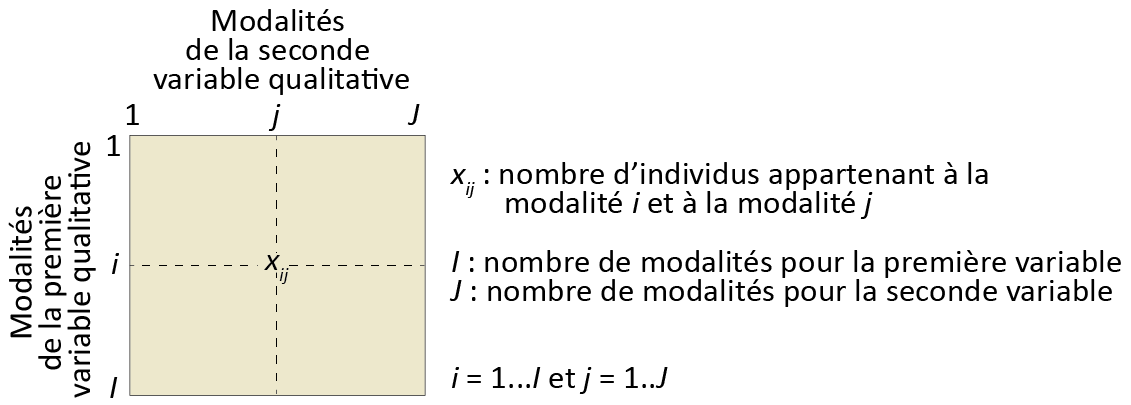
\includegraphics[width=0.7\linewidth]{images/analysesfactorielles/AnalysesFactoriellesTabAFC} 

}

\caption{Tableau de contingence pour une AFC}\label{fig:AnalysesFactoriellesTabAFCFig}
\end{figure}

À titre de rappel (section \ref{sect1212}), l'AFC a été développée par le statisticien français Jean-Paul Benzécri (\protect\hyperlink{ref-benzecri1973analyse}{1973}). Cela explique qu'elle est souvent enseignée et utilisée en sciences sociales dans les universités francophones, mais plus rarement dans les universités anglophones. Pourtant, les applications de l'AFC sont nombreuses dans différentes disciplines des sciences sociales comme illustrées avec les exemples suivants~:

\begin{itemize}
\tightlist
\item
  En géographie, les modalités de la première variable du tableau de contingence sont souvent des entités spatiales (par exemple, régions, municipalités, quartiers, etc.) croisées avec les modalités d'une autre variable qualitative (catégories socioprofessionnelles, modes de transport, tranches de revenu des ménages ou des individus, etc.).
\item
  En économie régionale, nous pourrions vouloir explorer un tableau de contingence croisant des entités spatiales (par exemple, MRC au Québec, départements en France) et les effectifs d'emplois pour différents secteurs d'activité.
\item
  En sciences politiques, le recours à l'AFC peut être intéressant pour explorer les résultats d'une élection. Les deux variables qualitatives pourraient être les \emph{circonscriptions électorales} et les \emph{partis politiques}. Le croisement des lignes et des colonnes du tableau de contingence représenterait le nombre de votes obtenus par un parti politique \emph{j} dans la circonscription électorale \emph{i}. Appliquer une AFC sur un tel tableau de contingence permettrait de révéler les ressemblances entre les différents partis politiques et celles entre les circonscriptions électorales.
\end{itemize}

\begin{bloc_attention}
\textbf{Application d'une ACP sur un tableau de contingence transformé en un tableau avec les pourcentages en ligne~: un bien mauvais calcul\ldots{}}

Il pourrait être tentant de transformer le tableau de contingence initial (tableau~\ref{tab:encadreAFCACP1}) en un tableau avec les pourcentages en lignes (tableau~\ref{tab:encadreAFCACP2}) afin de lui appliquer une analyse en composantes principales. Une telle démarche a deux inconvénients majeurs~: chacune des modalités de la première variable qualitative (\emph{I}) aurait alors le même poids; chacune des modalités de la deuxième variable (\emph{J}) aurait aussi le même poids. Or, à la lecture des marges en ligne et en colonne au tableau~\ref{tab:encadreAFCACP1}, il est clair que la modalité \texttt{j1} et \texttt{i1} comprennent plus bien d'individus que les autres modalités respectives.

Si nous reprenons le dernier exemple applicatif, cela signifierait que le même poids sera accordé à chaque parti puisque les variables sont centrées réduites en ACP (moyenne~=~0 et variance~=~1). Autrement dit, les grands partis traditionnels seraient ainsi sur le pied d'égalité que les autres partis. Aussi, chaque circonscription électorale aurait le même poids bien que certaines comprennent bien plus d'électeurs et d'électrices que d'autres.

\end{bloc_attention}

\begin{table}[H]

\caption{\label{tab:encadreAFCACP1}Exemple de tableau de contingence pour l'AFC}
\centering
\fontsize{8}{10}\selectfont
\begin{tabular}[t]{lrrrrrr}
\toprule
  & j1 & j2 & j3 & j4 & j5 & Marge (ligne)\\
\midrule
i1 & 357 060 & 22 010 & 276 625 & 65 000 & 29 415 & 750 110\\
i2 & 427 530 & 26 400 & 295 860 & 69 410 & 30 645 & 849 845\\
i3 & 147 500 & 6 545 & 34 545 & 4 415 & 1 040 & 194 045\\
i4 & 128 520 & 6 405 & 42 925 & 6 565 & 2 670 & 187 085\\
Marge (colonne) & 1 060 610 & 61 360 & 649 955 & 145 390 & 63 770 & 1 981 085\\
\bottomrule
\end{tabular}
\end{table}

\textbackslash begin\{table\}{[}H{]}

\textbackslash caption\{\label{tab:encadreAFCACP2}Exemple d'un tableau de contingence transformé (\% en ligne) pour l'ACP\}
\centering
\fontsize{8}{10}\selectfont

\begin{tabular}[t]{lrrrrr}
\toprule
  & V1 & V2 & V3 & V4 & V5\\
\midrule
i1 & 47,6 & 2,9 & 36,9 & 8,7 & 3,9\\
i2 & 50,3 & 3,1 & 34,8 & 8,2 & 3,6\\
i3 & 76,0 & 3,4 & 17,8 & 2,3 & 0,5\\
i4 & 68,7 & 3,4 & 22,9 & 3,5 & 1,4\\
\bottomrule
\end{tabular}

\textbackslash end\{table\}

\hypertarget{sect1231}{%
\subsection{Recherche d'une simplification basée sur la distance du khi-deux}\label{sect1231}}

Sur le plan mathématique et des objectifs visés, l'AFC est similaire à l'ACP puisqu'elle permet d'explorer un tableau de trois façons~: 1) en montrant les ressemblances entre un ensemble d'individus (\emph{I}), 2) en révélant les liaisons entre les variables (\emph{J}) et 3) en résumant le tout avec des variables synthétiques. Toutefois avec l'AFC, les ensembles \emph{I} et \emph{J} sont les modalités de deux variables qualitatives (dont le croisement forme un tableau de contingence) et elle est basée sur la distance du khi-deux (et non sur la distance euclidienne comme en ACP).

Ainsi, avec la distance du khi-deux, la proximité (ressemblance) entre deux lignes (\emph{i} et \emph{l}) et deux colonnes (\emph{j} et \emph{k}) est mesurée comme suit~:

\footnotesize

\begin{equation}
d_{\chi_{il}^2} = \sum_j \frac{1}{f_{.j}}(\frac{f_{ij}}{f_{i.}}-\frac{f_{lj}}{f_{l.}})^2
\label{eq:khideuxlignes}
\end{equation}
\normalsize

\footnotesize

\begin{equation}
d_{\chi_{jk}^2} = \sum_i \frac{1}{f_{i.}}(\frac{f_{ij}}{f_{.j}}-\frac{f_{ik}}{f_{.k}})^2
\label{eq:khideuxcolonnes}
\end{equation}
\normalsize

Prenons un exemple fictif pour calculer ces deux distances. Le tableau \ref{tab:afcdataex1} comprend trois modalités en ligne (\emph{I}) et trois autres en colonnes (\emph{J}). Le total des effectifs de ce tableau de contingence est égal à 1~665.

\begin{table}

\caption{\label{tab:afcdataex1}Données brutes du tableau de contingence}
\centering
\fontsize{8}{10}\selectfont
\begin{tabular}[t]{lcccc}
\toprule
  & j1 & j2 & j3 & Total (ligne)\\
\midrule
i1 & 360 & 65 & 275 & 700\\
i2 & 420 & 70 & 290 & 780\\
i3 & 145 & 5 & 35 & 185\\
Total (colonne) & 925 & 140 & 600 & 1 665\\
\bottomrule
\end{tabular}
\end{table}

À partir des données brutes, il est facile de construire deux tableaux~: le profil des lignes et le profil des colonnes (tableau \ref{tab:afcProfilsLignesCols}), c'est-à-dire les proportions en ligne et en colonne.

\begin{table}

\caption{\label{tab:afcProfilsLignesCols}Profils des lignes et des colonnes}
\centering
\fontsize{8}{10}\selectfont
\begin{tabular}[t]{ccccc}
\toprule
 & j1 & j2 & j3 & Total\\
\midrule
\addlinespace[0.3em]
\multicolumn{5}{l}{\textbf{Profil des lignes}}\\
\hspace{1em}i1 & 0,514 & 0,093 & 0,393 & 1\\
\hspace{1em}i2 & 0,538 & 0,090 & 0,372 & 1\\
\hspace{1em}i3 & 0,784 & 0,027 & 0,189 & 1\\
\addlinespace[0.3em]
\multicolumn{5}{l}{\textbf{Profils des colonnes}}\\
\hspace{1em}i1 & 0,389 & 0,464 & 0,458 & \\
\hspace{1em}i2 & 0,454 & 0,500 & 0,483 & \\
\hspace{1em}i3 & 0,157 & 0,036 & 0,058 & \\
\hspace{1em}Total & 1,000 & 1,000 & 1,000 & \\
\bottomrule
\end{tabular}
\end{table}

En divisant les valeurs du tableau \ref{tab:afcdataex1} par le grand total (1~665), nous obtenons tous les termes utilisés dans les équations \eqref{eq:khideuxlignes} et \eqref{eq:khideuxcolonnes} au tableau \ref{tab:afcdataex2}~:

\begin{itemize}
\tightlist
\item
  Les fréquences relatives dénommées \(f_{ij}\).
\item
  La marge \(fi.\) est égale à la somme des fréquences relatives en ligne.
\item
  La marge \(f.j\) est égale à la somme des fréquences relatives en colonne.
\item
  La somme de toutes les fréquences relatives est donc égale à 1, soit \(\sum{f_{i.}}\) ou \(\sum{f_{.j}}\).
\end{itemize}

\begin{table}

\caption{\label{tab:afcdataex2}Données relatives du tableau de contingence (fij)}
\centering
\fontsize{8}{10}\selectfont
\begin{tabular}[t]{lrrrr}
\toprule
  & j1 & j2 & j3 & Total (fi.)\\
\midrule
i1 & 0,216 & 0,039 & 0,165 & 0,420\\
i2 & 0,252 & 0,042 & 0,174 & 0,468\\
i3 & 0,087 & 0,003 & 0,021 & 0,111\\
Total (f.j) & 0,556 & 0,084 & 0,360 & 1,000\\
\bottomrule
\end{tabular}
\end{table}

Il est possible de calculer les distances entre les différentes modalités de \emph{I} en appliquant l'équation \eqref{eq:khideuxlignes}; par exemple, la distance entre les observations \texttt{i1} et \texttt{i2} est égale à~:

\(d_{(i1,i2)}=\frac{\mbox{1}}{\mbox{0,556}}(\mbox{0,216}-\mbox{0,252})^2+\frac{\mbox{1}}{\mbox{0,084}}(\mbox{0,039}-\mbox{0,042})^2+ \frac{\mbox{1}}{\mbox{0,360}}(\mbox{0,165}-\mbox{0,174})^2=\mbox{0,003}\)

Avec l'équation \eqref{eq:khideuxcolonnes}, la distance entre les modalités \texttt{j1} et \texttt{j2} de \emph{J} est égale à~:

\(d_{(j1,j2)}=\frac{\mbox{1}}{\mbox{0,420}}(\mbox{0,216}-\mbox{0,039})^2+ \frac{\mbox{1}}{\mbox{0,468}}(\mbox{0,252}-\mbox{0,042})^2 + \frac{\mbox{1}}{\mbox{0,111}}(\mbox{0,087}-\mbox{0,003})^2=\mbox{0,233}\)

À la lecture du tableau \ref{tab:MatriceDistKhi}, les modalités les plus sont semblables sont
\texttt{i1} et \texttt{i2} (0,003) pour \emph{I} et \texttt{j1} et \texttt{j3} (0,058) pour \emph{J}.

\begin{table}

\caption{\label{tab:MatriceDistKhi}Distances du khi-deux entre les modalités I et les modalités J}
\centering
\fontsize{8}{10}\selectfont
\begin{tabular}[t]{cccccccc}
\toprule
Ind. & i1 & i2 & i3 & Col. & j1 & j2 & j3\\
\midrule
i1 & 0,000 & 0,003 & 0,103 & j1 & 0,000 & 0,233 & 0,058\\
i2 & 0,003 & 0,000 & 0,132 & j2 & 0,233 & 0,000 & 0,078\\
i3 & 0,103 & 0,132 & 0,000 & j3 & 0,058 & 0,078 & 0,000\\
\bottomrule
\end{tabular}
\end{table}

Finalement, l'approche pour déterminer les axes factoriels de l'AFC est similaire à celle de l'AFC~: les axes factoriels sont les droites orthogonales qui minimisent les distances aux points du profil des lignes, excepté que la métrique pour mesurer ces distances est celle du khi-deux (et non celle la distance euclidienne comme ACP). Pour plus détail sur le calcul de ces axes (notamment les formulations matricielles), consultez notamment Benzécri (\protect\hyperlink{ref-benzecri1973analyse}{1973}), Escofier et Pagès (\protect\hyperlink{ref-escofier1998analyses}{1998}) et Lebart et al.~(\protect\hyperlink{ref-lebart1995statistique}{1995}).

\hypertarget{sect1232}{%
\subsection{Aides à l'interprétation}\label{sect1232}}

Pour illustrer les aides à l'interprétation de l'AFC, nous utilisons un jeu de données spatiales extrait du \href{https://www12.statcan.gc.ca/census-recensement/2016/dp-pd/prof/index.cfm?Lang=F}{profil du recensement de 2016 de Statistique Canada} pour les secteurs de recensement de l'île de Montréal. La liste des modalités des variables qu'il comprend est reportée au tableau \ref{tab:dataAfc}. L'AFC est calculée sur un tableau de contingence croisant les secteurs de recensement (lignes) et les modalités d'une variable relative au mode de transport utilisé pour les déplacements domicile-travail (colonnes). Ces modalités sont cartographiées à la figure \ref{fig:cartovarAFC}.

\begin{table}

\caption{\label{tab:dataAfc}Jeu de données utilisé pour l'analyse factorielle des correspondances}
\centering
\fontsize{8}{10}\selectfont
\begin{tabular}[t]{llr}
\toprule
Nom & Intitulé & Somme\\
\midrule
\addlinespace[0.3em]
\multicolumn{3}{l}{\textbf{Modalités de la variable utilisée dans l'AFC (mode de transport)}}\\
\hspace{1em}VehCond & Véhicule motorisé (conducteur·trice) & 427 560\\
\hspace{1em}VehPass & Véhicule motorisé (passager·ère) & 26 490\\
\hspace{1em}TranspC & Transport en commun & 295 800\\
\hspace{1em}Apied & À pied & 69 330\\
\hspace{1em}Velo & Bicyclette & 30 615\\
\hspace{1em}AutreMoyen & Autre moyen & 7 750\\
\addlinespace[0.3em]
\multicolumn{3}{l}{\textbf{Modalités de la variable supplémentaire (durée du trajet)}}\\
\hspace{1em}T15min & Moins de 15 minutes & 130 435\\
\hspace{1em}T1529min & 15 à 29 minutes & 287 500\\
\hspace{1em}T3044min & 30 à 44 minutes & 244 425\\
\hspace{1em}T4559min & 45 à 59 minutes & 107 065\\
\hspace{1em}T60plus & 60 minutes et plus & 88 050\\
\bottomrule
\end{tabular}
\end{table}

\begin{figure}

{\centering \includegraphics[width=1\linewidth]{livre_statistique_Phil_Jere_clean_files/figure-latex/cartovarAFC-1} 

}

\caption{Cartographie des modalités de la variable mode de transport utilisée pour l'AFC}\label{fig:cartovarAFC}
\end{figure}

\hypertarget{sect12321}{%
\subsubsection{Résultats de l'AFC pour les valeurs propres}\label{sect12321}}

Avant de calculer l'AFC, il convient de vérifier s'il y a bien dépendance entre les modalités des deux variables qualitatives. En effet, si les deux variables sont indépendantes, il n'est pas nécessaire de résumer le tableau de contingence avec une AFC. Pour ce faire, nous utilisons le test du khi-deux largement décrit à la section \ref{sect052}. Les résultats de ce test signalent qu'il existe des associations entre les modalités des deux variables (\(\chi\)~=~203~971, p~\textless~0,001, tableau \ref{tab:dataafckhi2}). Nous pouvons donc appliquer une AFC sur ce tableau de contingence.

\begin{table}

\caption{\label{tab:dataafckhi2}Résultats du test du khi-deux sur le tableau de contingence}
\centering
\fontsize{8}{10}\selectfont
\begin{tabular}[t]{lr}
\toprule
Mesure & Valeur\\
\midrule
Modalités \textit{I} (secteurs de recensement) & 521,00\\
Modalités \textit{J} (variable mode de transport) & 6,00\\
Somme des données brutes ($n_{ij}$) & 857 545,00\\
Khi-deux ($\chi^2$) & 207 129,27\\
Degrés de liberté, soit $(c-1)\times(l-1)$ & 2 600,00\\
\addlinespace
Valeur de \textit{p} & 0,00\\
Coefficient Phi au carré ($\phi^2=\chi^2 / n_{ij})$ & 0,24\\
\bottomrule
\end{tabular}
\end{table}

Nous avons vu qu'en ACP normée (section \ref{sect12221}), la somme des valeurs propres est égale au nombre de variables puisqu'elles sont centrées réduites. Par contre, en AFC, cette somme est égale à l'inertie totale du tableau de contingence, c'est-à-dire à la valeur du khi-deux divisée par le nombre total des effectifs bruts (soit le coefficient phi au carré, \(\phi^2\)) (section \ref{sect052}). Le tableau \ref{tab:dataafcValeurPropres} permet de vérifier que la somme des valeurs propres est bien égale au coefficient phi au carré~:

\(\mbox{0,156}+\mbox{0,046}+\mbox{0,031}+\mbox{0,004}+\mbox{0,004} = \mbox{0,24} \\ \phi^2 = \chi^2 / n_{ij}=\mbox{203 971}/ \mbox{849 795} = \mbox{0,24}\)

\begin{table}

\caption{\label{tab:dataafcValeurPropres}Résultats de l'AFC pour les valeurs propres}
\centering
\fontsize{8}{10}\selectfont
\begin{tabular}[t]{rrrr}
\toprule
Axe factoriel & Valeur propre & Pourcentage & Pourc. cumulé\\
\midrule
1 & 0,156 & 64,590 & 64,590\\
2 & 0,046 & 19,250 & 83,840\\
3 & 0,031 & 12,995 & 96,835\\
4 & 0,004 & 1,683 & 98,518\\
5 & 0,004 & 1,482 & 100,000\\
\bottomrule
\end{tabular}
\end{table}

\textbf{Combien d'axes d'une AFC faut-il retenir?}

\begin{itemize}
\item
  \textbf{Approche statistique}. Mike Bendixen (\protect\hyperlink{ref-bendixen1995compositional}{1995}), cité dans l'excellent site \href{http://www.sthda.com/french/articles/38-methodes-des-composantes-principales-dans-r-guide-pratique/74-afc-analyse-factorielle-des-correspondances-avec-r-l-essentiel/\#valeurs-propres-variances}{STDA}, propose deux critères pour sélectionner les premiers axes d'une AFC~: \(c_1= 1 / (l-1) \times 100\) et \(c_2= 1 / (c-1) \times 100\) avec \emph{l} et \emph{c} étant respectivement les nombres de modalités en ligne et en colonne. Autrement dit, lorsque les données sont distribuées aléatoirement, la valeur propre en pourcentage devrait être égale à \(c_1\) et celle de l'axe factoriel moyen à \(c_2\). Par conséquent, nous pourrions retenir uniquement les axes dont les valeurs propres en pourcentage excèdent~: \(c_1 = \mbox{1}/(\mbox{521}-\mbox{1})\times \mbox{100}=\mbox{0,19 }%
  \) et \(c_2=\mbox{1}/(\mbox{6}-\mbox{1})\times \mbox{100}=\mbox{20 }%
  \). En appliquant ces deux critères, seul premier axe factoriel qui résume 65,6~\% mériterait d'être retenu.
\item
  \textbf{Approche empirique} basée sur la lecture des pourcentages et des pourcentages cumulés. Nous retenons uniquement les deux premières composantes qui résument 85~\% de la variance totale. Pour faciliter le choix du nombre d'axes avec cette approche empirique, il est fortement conseillé de construire un histogramme à partir des valeurs propres, soit brutes, soit en pourcentages, soit en pourcentages cumulés (figure~\ref{fig:afcGraphVP}).
\end{itemize}

\begin{figure}

{\centering \includegraphics[width=0.8\linewidth]{livre_statistique_Phil_Jere_clean_files/figure-latex/afcGraphVP-1} 

}

\caption{Histogramme des valeurs propres de l'AFC}\label{fig:afcGraphVP}
\end{figure}

\hypertarget{sect12322}{%
\subsubsection{Résultats de l'AFC pour les variables et les individus}\label{sect12322}}

Comme pour l'ACP, nous retrouvons les trois mêmes mesures pour les variables et les individus~: 1)~les coordonnées factorielles, 2)~les contributions et 3)~les cosinus carrés.

\begin{bloc_objectif}
\textbf{Compréhension des axes factoriels de l'AFC~: une étape essentielle, incontournable\ldots{}}

Comme en ACP, l'analyse des trois mesures (coordonnées, contributions et cosinus carrés) pour les variables et les individus doit vous permettre de comprendre la signification des axes factoriels retenus de l'AFC. Cette étape d'interprétation est essentielle afin de qualifier les variables latentes (axes factoriels, variables synthétiques) produites par l'AFC.

\end{bloc_objectif}

\begin{itemize}
\tightlist
\item
  \textbf{Les coordonnées factorielles} sont simplement les projections des points-lignes et de points-colonnes sur les axes de l'AFC. Tant pour les lignes que pour les colonnes, ces coordonnées bénéficient de deux propriétés intéressantes. Premièrement pour chaque axe factoriel \emph{k}, la somme du produit des marges des variables (\(f.j\), colonnes) ou des individus (\(fi.\), lignes) avec leurs coordonnées respectives (\(C^k_j\) et \(C^k_i\)) est égale à 0 (eq.~\eqref{eq:CoordPropr1}). Deuxièmement, pour chaque axe factoriel \emph{k}, la somme des produits entre les marges (en ligne et en colonne) et les coordonnées au carré (en ligne et en colonne) est égale à la valeur propre de l'axe (eq.~\eqref{eq:CoordPropr2}).
\end{itemize}

\footnotesize

\begin{equation}
\sum{f.j (C^k_j)}= 0 \text{ et} \sum{fi. (C^k_i)}= 0
\label{eq:CoordPropr1}
\end{equation}
\normalsize

\footnotesize

\begin{equation}
\sum{fi. (C^k_i)^2}= \mu_k \text{ et} \sum{f.j (C^k_j)^2}= \mu_k
\label{eq:CoordPropr2}
\end{equation}
\normalsize

En guise d'exemple, le tableau \ref{tab:dataafcCoordVars2} permet de vérifier les deux propriétés des coordonnées pour les variables. Les sommes de \({f.j (C^k_j)}\) pour les axes~1 et~2 sont bien égales à 0; et les sommes de \({f.j (C^k_j)^2}\) pour les axes~1 et~2 sont bien égales aux valeurs propres de ces deux axes, soit 0,156 et 0,046 (comparez ces valeurs avec celles reportées au tableau \ref{tab:dataafcValeurPropres} plus haut).

\begin{table}

\caption{\label{tab:dataafcCoordVars2}Vérification des deux propriétés des coordonnées factorielles pour les variables}
\centering
\fontsize{8}{10}\selectfont
\begin{tabular}[t]{lrrrrrrr}
\toprule
\multicolumn{2}{c}{ } & \multicolumn{2}{c}{Coord.} & \multicolumn{2}{c}{f.j x Coord.} & \multicolumn{2}{c}{f.j x Coord2} \\
\cmidrule(l{3pt}r{3pt}){3-4} \cmidrule(l{3pt}r{3pt}){5-6} \cmidrule(l{3pt}r{3pt}){7-8}
Modalité & f.j & 1 & 2 & 1 & 2 & 1 & 2\\
\midrule
VehCond & 0,499 & -0,329 & 0,077 & -0,164 & 0,038 & 0,054 & 0,003\\
VehPass & 0,031 & -0,255 & 0,081 & -0,008 & 0,003 & 0,002 & 0,000\\
TranspC & 0,345 & 0,208 & -0,229 & 0,072 & -0,079 & 0,015 & 0,018\\
Apied & 0,081 & 0,813 & 0,545 & 0,066 & 0,044 & 0,053 & 0,024\\
Velo & 0,036 & 0,938 & -0,187 & 0,033 & -0,007 & 0,031 & 0,001\\
\addlinespace
AutreMoyen & 0,009 & 0,142 & 0,078 & 0,001 & 0,001 & 0,000 & 0,000\\
Somme & 1,000 &  &  & 0,000 & 0,000 & 0,156 & 0,046\\
\bottomrule
\end{tabular}
\end{table}

\begin{bloc_attention}
Contrairement à l'ACP, les coordonnées factorielles pour les variables en ACF ne sont pas les coefficients de corrélation de Pearson des variables sur les axes!

\end{bloc_attention}

\begin{itemize}
\tightlist
\item
  \textbf{Les contributions} des variables ou des lignes en AFC permettent des repérer celles qui contribuent le plus à la formation des axes factoriels (de manière analogue à l'ACP). Pour un axe donné, leur sommation est égale à~100~\%. Elles s'obtiennent en multipliant la coordonnée au carré avec la marge et en divisant le tout par la valeur propre de l'axe (eq.~\eqref{eq:CtrAFCVar} et~\eqref{eq:CtrAFCInd}).
\end{itemize}

\footnotesize

\begin{equation}
\mbox{Ctr}_j^k =\frac{f.j(C^k_j)^2}{\mu_{k}}\times 100
\label{eq:CtrAFCVar}
\end{equation}
\normalsize

\footnotesize

\begin{equation}
\mbox{Ctr}_i^k =\frac{fi.(C^k_i)^2}{\mu_{k}}\times 100
\label{eq:CtrAFCInd}
\end{equation}
\normalsize

\begin{itemize}
\tightlist
\item
  \textbf{Les cosinus carrés} (Cos\textsuperscript{2}) (appelés aussi les qualités de représentation sur un axe) permettent de repérer le ou les axes qui concourent le plus à donner un sens aux variables et aux individus (de manière analogue à l'ACP). Pour une variable ou un individu, la sommation des Cos\textsuperscript{2} pour tous les axes de l'AFC est aussi égale à 1.
\end{itemize}

\textbf{Interprétation des résultats pour les variables}

Analysons maintenant, ces trois statistiques pour les variables pour les deux premiers axes de l'AFC (tableau~\ref{tab:dataafcCoordVars} et figure~\ref{fig:afc1erplanfactVars}).

Pour l'axe~1, résumant 65~\% de la variance, trois modalités concourent à sa formation~: \texttt{VehCond} (34,69~\%), \texttt{Apied} (34,25~\%) et \texttt{Velo} (20,13~\%). À la lecture des coordonnées factorielles sur cet axe, les modes de transport relatifs aux véhicules motorisés (\texttt{VehCond}~=~-0,33 et \texttt{VehPass}~=~-0,25) s'opposent clairement aux modes actifs (\texttt{Apied}~=~0,81 et \texttt{Velo}~=~0,94), constat qu'il est possible de confirmer visuellement avec la figure~\ref{fig:afc1erplanfactVars}). La modalité \texttt{VehCond} a d'ailleurs la plus forte valeur de Cos\textsuperscript{2} sur cet axe (0,92), ce qui signale, sans l'ombre d'un doute, que l'axe~1 est celui qui donner le plus de sens à cette modalité.

Puisque l'axe~2 résume une partie beaucoup plus limitée de la variance du tableau (19,25~\%), il n'est pas étonnant qu'un nombre plus limité de modalités concourent à sa formation~: seules les contributions de la modalité \texttt{Apied} (51,68~\%) et secondairement \texttt{VehPass} (38,81~\%) sont importantes. Leurs coordonnées factorielles s'opposent d'ailleurs sur cet axe (respectivement 0,81 et 0,21).

\begin{table}

\caption{\label{tab:dataafcCoordVars}Résultats de l'AFC pour les variables}
\centering
\fontsize{8}{10}\selectfont
\begin{tabular}[t]{lrrrrrr}
\toprule
\multicolumn{1}{c}{ } & \multicolumn{2}{c}{Coordonnées} & \multicolumn{2}{c}{Cosinus carrés} & \multicolumn{2}{c}{Contributions (\%)} \\
\cmidrule(l{3pt}r{3pt}){2-3} \cmidrule(l{3pt}r{3pt}){4-5} \cmidrule(l{3pt}r{3pt}){6-7}
Modalité & 1 & 2 & 1 & 2 & 1 & 2\\
\midrule
VehCond & -0,33 & 0,08 & 0,92 & 0,05 & 34,69 & 6,33\\
VehPass & -0,25 & 0,08 & 0,34 & 0,03 & 1,28 & 0,44\\
TranspC & 0,21 & -0,23 & 0,39 & 0,47 & 9,53 & 38,81\\
Apied & 0,81 & 0,54 & 0,67 & 0,30 & 34,25 & 51,61\\
Velo & 0,94 & -0,19 & 0,56 & 0,02 & 20,13 & 2,69\\
\addlinespace
AutreMoyen & 0,14 & 0,08 & 0,05 & 0,01 & 0,12 & 0,12\\
\bottomrule
\end{tabular}
\end{table}

\begin{figure}

{\centering \includegraphics[width=0.75\linewidth]{livre_statistique_Phil_Jere_clean_files/figure-latex/afc1erplanfactVars-1} 

}

\caption{Premier plan factoriel de l'AFC pour les variables}\label{fig:afc1erplanfactVars}
\end{figure}

\textbf{Interprétation des résultats pour les individus}

\begin{bloc_notes}
\textbf{Premier plan factoriel pour les variables et les individus}

Lorsque le jeu de données comprend à la fois peu de modalités en lignes et en colonnes, il est judicieux de les représenter simultanément sur le premier plan factoriel (axe~1 et~2). Pour ce faire, vous pouvez utiliser la fonction \texttt{fviz\_ca\_biplot} du \emph{package} \texttt{factoextra}.

\end{bloc_notes}

Étant donné que notre jeu de données comprend 521~secteurs de recensement, nous proposons ici de cartographier les coordonnées factorielles des individus pour les deux premiers axes de l'AFC (figure~\ref{fig:afc1erplanfactInds2}). Pour l'axe~1, les secteurs de recensement à l'est et l'ouest de l'île de Montréal présentent les coordonnées les plus fortement négatives (en rouge); dans ces zones, l'usage des véhicules motorisés pour des déplacements domicile-travail est certainement surreprésenté, comparativement aux modes actifs. À l'inverse, dans les secteurs de recensement du centre de l'île présentant de fortes valeurs positives (en rouge), le recours aux modes de transports actifs (marche et vélo) est bien plus important, toutes proportions gardées. Quant à la cartographie des coordonnées pour l'axe~2, elle permet surtout de repérer quelques secteurs de recensement autour du centre-ville (très fortes valeurs positives en vert) où les déplacements domicile-travail à pied sont plus fréquents, toutes proportions gardées.

En résumé, suite à l'analyse des coordonnées factorielles des variables et des individus, nous pouvons conclure que le premier axe est certainement le plus intéressant puisqu'il permet d'opposer l'usage des modes de transports motorisés versus les modes de transports actifs pour les déplacements domicile-travail sur l'île de Montréal. Cette nouvelle variable synthétique (variable latente) pourrait ainsi être introduite des analyses subséquentes (par exemple, dans un modèle de régression). Cela démontre, qu'au même titre que l'ACP, l'AFC une méthode de réduction de données puisque nous sommes passés d'un tableau comprenant 512 secteurs de recensement et six modalités à un tableau comprend une seule variable synthétique (axe~1).

\begin{figure}

{\centering \includegraphics[width=0.85\linewidth]{livre_statistique_Phil_Jere_clean_files/figure-latex/afc1erplanfactInds2-1} 

}

\caption{Cartographie de coordonnées factorielles des individus pour l'ACF}\label{fig:afc1erplanfactInds2}
\end{figure}

\begin{bloc_aller_loin}

\textbf{Ajout de modalités supplémentaires dans une analyse des correspondances (AFC)}.

Comme pour l'ACP, il est possible d'ajouter des variables et des individus supplémentaires une fois l'AFC calculée. En guise d'illustration, nous avons ajouté à l'AFC précédemment analysée des modalités relatives à la durée des temps de déplacements~: moins de 15 minutes, 15 à 29, 30 à 44, 45 à 59, 60 minutes et plus. Sans surprise, sur le premier plan factoriel à la figure~\ref{fig:afc1erplanfactInds2}, cette dernière modalité, représentant les trajets les plus longs, est la plus proche des modalités relatives à l'usage des véhicules motorisés (\texttt{VehCond} et \texttt{VehPass}).

\begin{figure}[H]

{\centering \includegraphics[width=0.75\linewidth]{livre_statistique_Phil_Jere_clean_files/figure-latex/afcAjoutModalites-1} 

}

\caption{Ajout de modalités supplémentaires sur le premier plan factoriel de l'AFC}\label{fig:afcAjoutModalites}
\end{figure}


\end{bloc_aller_loin}

\hypertarget{sect1233}{%
\subsection{Mise en œuvre dans R}\label{sect1233}}

\hypertarget{sect12331}{%
\subsubsection{\texorpdfstring{Calcul d'une AFC avec \texttt{FactoMineR}}{Calcul d'une AFC avec FactoMineR}}\label{sect12331}}

Plusieurs \emph{packages} permettent de calculer une AFC dans R, notamment \texttt{ca} (fonction \texttt{ca}), \texttt{MASS} (fonction \texttt{corresp}), \texttt{ade4} (fonction \texttt{dudi.coa}) et \texttt{FactoMineR} (fonction \texttt{CA}). De nouveau, nous utilisons \texttt{FactoMineR} couplé au \emph{package} \texttt{factoextra} pour réaliser rapidement des graphiques avec les résultats pour les variables et les coordonnées.

Pour calculer l'AFC, il suffit d'utiliser la fonction \texttt{CA} de \texttt{FactoMineR}, puis la fonction \texttt{summary(res.afc)} qui renvoie les résultats de l'AFC pour~:

\begin{itemize}
\tightlist
\item
  Les valeurs propres (section \texttt{Eigenvalues}) pour les axes factoriels (\texttt{Dim.1} à \texttt{Dim.n}) avec leur variance expliquée brute (\texttt{Variance}), en pourcentage (\texttt{\%\ of\ var.}) et en pourcentage cumulé (\texttt{Cumulative\ \%\ of\ var.}).
\item
  Les dix premières observations (section \texttt{Rows}) avec les coordonnées factorielles (\texttt{Dim.1} à \texttt{Dim.n}), les contributions (\texttt{ctr}) et les cosinus carrés (\texttt{cos2}). Pour accéder aux résultats pour toutes les observations, utilisez les fonctions \texttt{res.afc\$row} ou encore \texttt{res.afc\$row\$coord} (uniquement les coordonnées factorielles), \texttt{res.afc\$row\$contrib} (uniquement les contributions) et \texttt{res.afc\$ind\$cos2} (uniquement les cosinus carrés).
\item
  Les colonnes (section \texttt{Columns}) avec les coordonnées factorielles (D\texttt{im.1} à \texttt{Dim.n}), les contributions (\texttt{ctr}) et les cosinus carrés (\texttt{cos2}).
\end{itemize}

\begin{Shaded}
\begin{Highlighting}[]
\CommentTok{# Chargement des packages}
\KeywordTok{library}\NormalTok{(FactoMineR)}
\KeywordTok{library}\NormalTok{(factoextra)}
\CommentTok{# Chargement des données}
\KeywordTok{load}\NormalTok{(}\StringTok{"data/analysesfactorielles/DonneesAFC.Rdata"}\NormalTok{)}

\CommentTok{# Avant de calculer l'AFC, il convient de vérifier si les deux variables}
\CommentTok{# qualitatives sont dépendantes avec le test du khi-deux}
\NormalTok{khideux <-}\StringTok{ }\KeywordTok{chisq.test}\NormalTok{(dfDonneesAFC[,}\DecValTok{1}\OperatorTok{:}\DecValTok{6}\NormalTok{])}
\KeywordTok{print}\NormalTok{(khideux)}
\end{Highlighting}
\end{Shaded}

\begin{verbatim}
## 
##  Pearson's Chi-squared test
## 
## data:  dfDonneesAFC[, 1:6]
## X-squared = 207129, df = 2600, p-value < 2.2e-16
\end{verbatim}

\begin{Shaded}
\begin{Highlighting}[]
\ControlFlowTok{if}\NormalTok{(khideux}\OperatorTok{$}\NormalTok{p.value }\OperatorTok{<=}\FloatTok{0.05}\NormalTok{)\{}
  \KeywordTok{cat}\NormalTok{(}\StringTok{"}\CharTok{\textbackslash{}n}\StringTok{La valeur de p < 0,05. Les variables sont dépendantes. Calculer l'AFC."}\NormalTok{)}
\NormalTok{\}}\ControlFlowTok{else}\NormalTok{ \{}
    \KeywordTok{cat}\NormalTok{(}\StringTok{"}\CharTok{\textbackslash{}n}\StringTok{La valeur de p > 0,05. Les variables sont indépendantes. Inutile de calculer l'AFC"}\NormalTok{)}
\NormalTok{\}}
\end{Highlighting}
\end{Shaded}

\begin{verbatim}
## 
## La valeur de p < 0,05. Les variables sont dépendantes. Calculer l'AFC.
\end{verbatim}

\begin{Shaded}
\begin{Highlighting}[]
\CommentTok{# Calcul de l'analyse des correspondances sur les six premières variables}
\NormalTok{res.afc <-}\StringTok{ }\KeywordTok{CA}\NormalTok{(dfDonneesAFC[,}\DecValTok{1}\OperatorTok{:}\DecValTok{6}\NormalTok{], }\DataTypeTok{graph=}\NormalTok{F)}
\CommentTok{# Affichage des résultats de la fonction CA}
\KeywordTok{print}\NormalTok{(res.afc)}
\end{Highlighting}
\end{Shaded}

\begin{verbatim}
## **Results of the Correspondence Analysis (CA)**
## The row variable has  521  categories; the column variable has 6 categories
## The chi square of independence between the two variables is equal to 207129.3 (p-value =  0 ).
## *The results are available in the following objects:
## 
##    name              description                   
## 1  "$eig"            "eigenvalues"                 
## 2  "$col"            "results for the columns"     
## 3  "$col$coord"      "coord. for the columns"      
## 4  "$col$cos2"       "cos2 for the columns"        
## 5  "$col$contrib"    "contributions of the columns"
## 6  "$row"            "results for the rows"        
## 7  "$row$coord"      "coord. for the rows"         
## 8  "$row$cos2"       "cos2 for the rows"           
## 9  "$row$contrib"    "contributions of the rows"   
## 10 "$call"           "summary called parameters"   
## 11 "$call$marge.col" "weights of the columns"      
## 12 "$call$marge.row" "weights of the rows"
\end{verbatim}

\begin{Shaded}
\begin{Highlighting}[]
\CommentTok{# Visualisation des marges en colonnes}
\KeywordTok{round}\NormalTok{(res.afc}\OperatorTok{$}\NormalTok{call}\OperatorTok{$}\NormalTok{marge.col,}\DecValTok{4}\NormalTok{)}
\end{Highlighting}
\end{Shaded}

\begin{verbatim}
##    VehCond    VehPass    TranspC      Apied       Velo AutreMoyen 
##     0.4986     0.0309     0.3449     0.0808     0.0357     0.0090
\end{verbatim}

\begin{Shaded}
\begin{Highlighting}[]
\CommentTok{# Visualisation des marges en lignes. Étant données que nous avons 521 individus, }
\CommentTok{# la ligne ci-dessous est en commentaire}
\CommentTok{# round(res.afc$call$marge.row,4)}

\CommentTok{# Sommaire des résultats de l'AFC}
\CommentTok{# Remarquez que la première ligne de ce sommaire est le résultat du khi-deux}
\KeywordTok{summary}\NormalTok{(res.afc)}
\end{Highlighting}
\end{Shaded}

\begin{verbatim}
## 
## Call:
## CA(X = dfDonneesAFC[, 1:6], graph = F) 
## 
## The chi square of independence between the two variables is equal to 207129.3 (p-value =  0 ).
## 
## Eigenvalues
##                        Dim.1   Dim.2   Dim.3   Dim.4   Dim.5
## Variance               0.156   0.046   0.031   0.004   0.004
## % of var.             64.590  19.250  12.995   1.683   1.482
## Cumulative % of var.  64.590  83.840  96.835  98.518 100.000
## 
## Rows (the 10 first)
##              Iner*1000    Dim.1    ctr   cos2    Dim.2    ctr   cos2    Dim.3
## 1          |     0.155 | -0.304  0.095  0.961 | -0.023  0.002  0.006 |  0.048
## 2          |     0.123 | -0.232  0.067  0.850 |  0.028  0.003  0.012 | -0.021
## 3          |     0.268 | -0.246  0.127  0.737 | -0.002  0.000  0.000 | -0.046
## 4          |     0.102 | -0.168  0.034  0.513 | -0.111  0.049  0.222 | -0.117
## 5          |     0.118 | -0.251  0.067  0.883 |  0.004  0.000  0.000 | -0.007
## 6          |     0.120 | -0.130  0.024  0.313 | -0.103  0.051  0.196 | -0.144
## 7          |     0.124 | -0.029  0.002  0.022 | -0.158  0.167  0.626 | -0.079
## 8          |     0.073 | -0.157  0.028  0.598 | -0.090  0.031  0.195 | -0.006
## 9          |     0.014 | -0.060  0.005  0.506 | -0.033  0.005  0.150 | -0.018
## 10         |     0.040 |  0.004  0.000  0.000 | -0.204  0.073  0.838 |  0.053
##               ctr   cos2  
## 1           0.012  0.024 |
## 2           0.003  0.007 |
## 3           0.022  0.026 |
## 4           0.080  0.246 |
## 5           0.000  0.001 |
## 6           0.146  0.380 |
## 7           0.061  0.155 |
## 8           0.000  0.001 |
## 9           0.002  0.048 |
## 10          0.007  0.056 |
## 
## Columns
##              Iner*1000    Dim.1    ctr   cos2    Dim.2    ctr   cos2    Dim.3
## VehCond    |    58.559 | -0.329 34.687  0.924 |  0.077  6.331  0.050 |  0.051
## VehPass    |     5.923 | -0.255  1.283  0.338 |  0.081  0.440  0.035 |  0.001
## TranspC    |    38.261 |  0.208  9.534  0.389 | -0.229 38.812  0.472 | -0.124
## Apied      |    79.193 |  0.813 34.252  0.675 |  0.545 51.610  0.303 | -0.147
## Velo       |    55.633 |  0.938 20.126  0.564 | -0.187  2.688  0.022 |  0.802
## AutreMoyen |     3.969 |  0.142  0.117  0.046 |  0.078  0.119  0.014 |  0.070
##               ctr   cos2  
## VehCond     4.141  0.022 |
## VehPass     0.000  0.000 |
## TranspC    16.995  0.139 |
## Apied       5.543  0.022 |
## Velo       73.180  0.413 |
## AutreMoyen  0.140  0.011 |
\end{verbatim}

\hypertarget{sect12332}{%
\subsubsection{\texorpdfstring{Exploration graphique des résultats de l'AFC avec \texttt{factoextra}}{Exploration graphique des résultats de l'AFC avec factoextra}}\label{sect12332}}

Comme pour l'ACP, \texttt{factoextra} dispose de plusieurs fonctions très intéressantes pour construire rapidement des graphiques avec les résultats de l'AFC. Premièrement, la syntaxe ci-dessous renvoie deux graphiques pour analyser les résultats des valeurs propres de l'AFC (figure~\ref{fig:factoextraAFC1}).

\begin{Shaded}
\begin{Highlighting}[]
\KeywordTok{library}\NormalTok{(factoextra)}
\KeywordTok{library}\NormalTok{(ggplot2)}
\KeywordTok{library}\NormalTok{(ggpubr)}

\CommentTok{# Nombre de modalités en lignes et en colonnes}
\NormalTok{ModalitesLig <-}\StringTok{ }\KeywordTok{nrow}\NormalTok{(dfDonneesAFC)}
\NormalTok{ModalitesCol <-}\StringTok{ }\KeywordTok{ncol}\NormalTok{(dfDonneesAFC[,}\DecValTok{1}\OperatorTok{:}\DecValTok{6}\NormalTok{])}
\CommentTok{# Critère statistique du profil moyen}
\NormalTok{critere2 <-}\StringTok{ }\KeywordTok{round}\NormalTok{(}\DecValTok{1}\OperatorTok{/}\NormalTok{(ModalitesCol}\DecValTok{-1}\NormalTok{)}\OperatorTok{*}\DecValTok{100}\NormalTok{,}\DecValTok{2}\NormalTok{)}
\NormalTok{texte <-}\StringTok{ }\KeywordTok{paste0}\NormalTok{(}\StringTok{"Critère pour le profil moyen : "}\NormalTok{, }\KeywordTok{as.character}\NormalTok{(critere2), }\StringTok{" %"}\NormalTok{)}
\CommentTok{# Graphique avec les valeurs propres}
\NormalTok{G1 <-}\StringTok{ }\KeywordTok{fviz_screeplot}\NormalTok{(res.afc, }\DataTypeTok{choice=}\StringTok{"eigenvalue"}\NormalTok{,}
               \DataTypeTok{ylab=}\StringTok{"Valeurs propres"}\NormalTok{,}
               \DataTypeTok{xlab=}\StringTok{"Axes factoriels"}\NormalTok{,}
               \DataTypeTok{main=}\StringTok{"Valeurs propres"}\NormalTok{)}
\NormalTok{G2 <-}\StringTok{ }\KeywordTok{fviz_screeplot}\NormalTok{(res.afc, }\DataTypeTok{choice=}\StringTok{"variance"}\NormalTok{, }\DataTypeTok{addlabels =} \OtherTok{TRUE}\NormalTok{, }\DataTypeTok{ylim =} \KeywordTok{c}\NormalTok{(}\DecValTok{0}\NormalTok{, }\DecValTok{70}\NormalTok{),}
                     \DataTypeTok{ylab=}\StringTok{"Variance expliquée (%)"}\NormalTok{,}
                     \DataTypeTok{xlab=}\StringTok{"Axes factoriels"}\NormalTok{,}
                     \DataTypeTok{main=}\StringTok{"Valeurs propres (%)"}\NormalTok{)}\OperatorTok{+}
\StringTok{  }\KeywordTok{geom_hline}\NormalTok{(}\DataTypeTok{yintercept =}\NormalTok{ c2, }\DataTypeTok{linetype =} \DecValTok{1}\NormalTok{, }\DataTypeTok{color =} \StringTok{"red"}\NormalTok{, }\DataTypeTok{size=}\DecValTok{1}\NormalTok{)}\OperatorTok{+}
\StringTok{  }\KeywordTok{annotate}\NormalTok{(}\DataTypeTok{geom=}\StringTok{"text"}\NormalTok{, }\DataTypeTok{x =}\NormalTok{ ModalitesCol}\FloatTok{-.5}\NormalTok{,}
          \DataTypeTok{y=}\NormalTok{ critere2}\OperatorTok{+}\DecValTok{3}\NormalTok{, }\DataTypeTok{label=}\NormalTok{texte, }
          \DataTypeTok{color=}\StringTok{"red"}\NormalTok{, }\DataTypeTok{hjust =} \DecValTok{1}\NormalTok{, }\DataTypeTok{size =} \DecValTok{4}\NormalTok{)}
\KeywordTok{ggarrange}\NormalTok{(G1, G2)}
\end{Highlighting}
\end{Shaded}

\begin{figure}

{\centering \includegraphics[width=0.75\linewidth]{livre_statistique_Phil_Jere_clean_files/figure-latex/factoextraAFC1-1} 

}

\caption{Graphiques pour les valeurs propres de l'AFC avec factoextra}\label{fig:factoextraAFC1}
\end{figure}

Avec les fonctions \texttt{fviz\_contrib} et \texttt{fviz\_cos2}, il est très facile de réaliser des histogrammes pour les contributions et les cosinus carrés pour les variables (colonnes) ou les individus (lignes), et ce avec le paramètre \texttt{choice\ =\ c("row",\ "col")} (figure~\ref{fig:acp1erplanfactVars2a}).

\begin{Shaded}
\begin{Highlighting}[]
\KeywordTok{library}\NormalTok{(factoextra)}
\KeywordTok{library}\NormalTok{(ggplot2)}
\KeywordTok{library}\NormalTok{(ggpubr)}
\NormalTok{VP1pct <-}\StringTok{ }\KeywordTok{round}\NormalTok{(res.afc}\OperatorTok{$}\NormalTok{eig[}\DecValTok{1}\NormalTok{,}\DecValTok{2}\NormalTok{],}\DecValTok{2}\NormalTok{)}
\NormalTok{VP2pct <-}\StringTok{ }\KeywordTok{round}\NormalTok{(res.afc}\OperatorTok{$}\NormalTok{eig[}\DecValTok{2}\NormalTok{,}\DecValTok{2}\NormalTok{],}\DecValTok{2}\NormalTok{)}
\NormalTok{G1 <-}\StringTok{ }\KeywordTok{fviz_contrib}\NormalTok{ (res.afc, }\DataTypeTok{choice =} \StringTok{"col"}\NormalTok{, }\DataTypeTok{axes =} \DecValTok{1}\NormalTok{, }\DataTypeTok{title=}\StringTok{"Axe 1"}\NormalTok{)}
\NormalTok{G2 <-}\StringTok{ }\KeywordTok{fviz_contrib}\NormalTok{ (res.afc, }\DataTypeTok{choice =} \StringTok{"col"}\NormalTok{, }\DataTypeTok{axes =} \DecValTok{2}\NormalTok{, }\DataTypeTok{title=}\StringTok{"Axe 2"}\NormalTok{)}
\KeywordTok{ggarrange}\NormalTok{(G1, G2, }\DataTypeTok{ncol =} \DecValTok{2}\NormalTok{, }\DataTypeTok{nrow =} \DecValTok{1}\NormalTok{)}
\end{Highlighting}
\end{Shaded}

\begin{figure}

{\centering \includegraphics[width=0.75\linewidth]{livre_statistique_Phil_Jere_clean_files/figure-latex/acp1erplanfactVars2a-1} 

}

\caption{Contributions des variables avec factoextra}\label{fig:acp1erplanfactVars2a}
\end{figure}

Quant aux \texttt{fviz\_ca\_col} et \texttt{fviz\_ca\_row}, elle permet rapidement de construire le premier plan factoriel pour les variables et les individus (figure~\ref{fig:afc1erplanfactVars2b}). Aussi, la fonction \texttt{fviz\_ca\_biplot} permettent de construire assi un plan factoriel, mais avec les lignes et les colonnes simultanément.

\begin{Shaded}
\begin{Highlighting}[]
\NormalTok{G3 <-}\StringTok{ }\KeywordTok{fviz_ca_col}\NormalTok{(res.afc,}
            \DataTypeTok{repel =} \OtherTok{TRUE}\NormalTok{,}
            \DataTypeTok{geom=} \KeywordTok{c}\NormalTok{(}\StringTok{"text"}\NormalTok{,}\StringTok{"point"}\NormalTok{),}
            \DataTypeTok{col.col =} \StringTok{"steelblue"}\NormalTok{,}
            \DataTypeTok{title =} \StringTok{"Mode de transport"}\NormalTok{,}
            \DataTypeTok{xlab=}\KeywordTok{paste0}\NormalTok{(}\StringTok{"Axe 1 ("}\NormalTok{, VP1pct, }\StringTok{" %)"}\NormalTok{),}
            \DataTypeTok{ylab=}\KeywordTok{paste0}\NormalTok{(}\StringTok{"Axe 2 ("}\NormalTok{, VP2pct, }\StringTok{" %)"}\NormalTok{))}
\NormalTok{G4 <-}\StringTok{ }\KeywordTok{fviz_ca_row}\NormalTok{(res.afc,}
            \DataTypeTok{repel =} \OtherTok{TRUE}\NormalTok{,}
            \DataTypeTok{geom=} \KeywordTok{c}\NormalTok{(}\StringTok{"point"}\NormalTok{),}
            \DataTypeTok{col.row =} \StringTok{"steelblue"}\NormalTok{,}
            \DataTypeTok{title =} \StringTok{"Secteurs de recensement"}\NormalTok{,}
            \DataTypeTok{xlab=}\KeywordTok{paste0}\NormalTok{(}\StringTok{"Axe 1 ("}\NormalTok{, VP1pct, }\StringTok{" %)"}\NormalTok{),}
            \DataTypeTok{ylab=}\KeywordTok{paste0}\NormalTok{(}\StringTok{"Axe 2 ("}\NormalTok{, VP2pct, }\StringTok{" %)"}\NormalTok{))}

\KeywordTok{ggarrange}\NormalTok{(G3, G4, }\DataTypeTok{ncol =} \DecValTok{2}\NormalTok{, }\DataTypeTok{nrow =} \DecValTok{1}\NormalTok{)}
\end{Highlighting}
\end{Shaded}

\begin{figure}

{\centering \includegraphics[width=0.75\linewidth]{livre_statistique_Phil_Jere_clean_files/figure-latex/afc1erplanfactVars2b-1} 

}

\caption{Premier plan factoriel de l'AFC pour les variables et les individus avec factoextra}\label{fig:afc1erplanfactVars2b}
\end{figure}

La syntaxe ci-dessous permet d'ajouter des modalités supplémentaires dans l'AFC et de constuire le graphique du premier plan factoriel (figure~\ref{fig:afcAjoutModalites2}).

\begin{Shaded}
\begin{Highlighting}[]
\CommentTok{# Les colonnes 7 à 11 sont mises comme des variables supplémentaires dans l'AFC}
\NormalTok{res.afc2 <-}\StringTok{ }\KeywordTok{CA}\NormalTok{(dfDonneesAFC, }\DataTypeTok{col.sup =} \DecValTok{7}\OperatorTok{:}\DecValTok{11}\NormalTok{, }\DataTypeTok{graph =} \OtherTok{FALSE}\NormalTok{)}
\NormalTok{VP1pct <-}\StringTok{ }\KeywordTok{round}\NormalTok{(res.afc2}\OperatorTok{$}\NormalTok{eig[}\DecValTok{1}\NormalTok{,}\DecValTok{2}\NormalTok{],}\DecValTok{2}\NormalTok{)}
\NormalTok{VP2pct <-}\StringTok{ }\KeywordTok{round}\NormalTok{(res.afc2}\OperatorTok{$}\NormalTok{eig[}\DecValTok{2}\NormalTok{,}\DecValTok{2}\NormalTok{],}\DecValTok{2}\NormalTok{)}
\KeywordTok{fviz_ca_col}\NormalTok{(res.afc2,}
            \DataTypeTok{repel =} \OtherTok{TRUE}\NormalTok{,}
            \DataTypeTok{geom=} \KeywordTok{c}\NormalTok{(}\StringTok{"text"}\NormalTok{,}\StringTok{"point"}\NormalTok{),}
            \DataTypeTok{col.col =} \StringTok{"steelblue"}\NormalTok{,}
            \DataTypeTok{title =} \StringTok{""}\NormalTok{,}
            \DataTypeTok{xlab=}\KeywordTok{paste0}\NormalTok{(}\StringTok{"Axe 1 ("}\NormalTok{, VP1pct, }\StringTok{" %)"}\NormalTok{),}
            \DataTypeTok{ylab=}\KeywordTok{paste0}\NormalTok{(}\StringTok{"Axe 2 ("}\NormalTok{, VP2pct, }\StringTok{" %)"}\NormalTok{))}
\end{Highlighting}
\end{Shaded}

\begin{figure}[H]

{\centering \includegraphics[width=0.75\linewidth]{livre_statistique_Phil_Jere_clean_files/figure-latex/afcAjoutModalites2-1} 

}

\caption{Ajout de modalités supplémentaires sur le premier plan factoriel l'AFC avec factoextra}\label{fig:afcAjoutModalites2}
\end{figure}

Finalement, la syntaxe ci-dessous permet de cartographier les coordonnées factorielles des individus de l'ACF (figure~\ref{fig:afc1erplanfactInds2B}).

\begin{Shaded}
\begin{Highlighting}[]
\KeywordTok{library}\NormalTok{(tmap)}
\KeywordTok{library}\NormalTok{(stringr)}
\NormalTok{dfAFCInd <-}\StringTok{ }\KeywordTok{data.frame}\NormalTok{(}\DataTypeTok{Coord =}\NormalTok{ res.afc}\OperatorTok{$}\NormalTok{row}\OperatorTok{$}\NormalTok{coord, }
                       \DataTypeTok{Cos2 =}\NormalTok{ res.afc}\OperatorTok{$}\NormalTok{row}\OperatorTok{$}\NormalTok{cos2, }
                       \DataTypeTok{Ctr =}\NormalTok{ res.afc}\OperatorTok{$}\NormalTok{row}\OperatorTok{$}\NormalTok{contrib)}
\KeywordTok{names}\NormalTok{(dfAFCInd) <-}\StringTok{ }\KeywordTok{str_replace}\NormalTok{(}\KeywordTok{names}\NormalTok{(dfAFCInd), }\StringTok{".Dim."}\NormalTok{, }\StringTok{"Comp"}\NormalTok{)}
\NormalTok{CartoAFC <-}\StringTok{ }\KeywordTok{cbind}\NormalTok{(sfDonneesAFC, dfAFCInd)}
\NormalTok{VP1pct <-}\StringTok{ }\KeywordTok{tofr}\NormalTok{(}\KeywordTok{round}\NormalTok{(res.afc}\OperatorTok{$}\NormalTok{eig[}\DecValTok{1}\NormalTok{,}\DecValTok{2}\NormalTok{],}\DecValTok{2}\NormalTok{))}
\NormalTok{VP2pct <-}\StringTok{ }\KeywordTok{tofr}\NormalTok{(}\KeywordTok{round}\NormalTok{(res.afc}\OperatorTok{$}\NormalTok{eig[}\DecValTok{2}\NormalTok{,}\DecValTok{2}\NormalTok{],}\DecValTok{2}\NormalTok{))}
\NormalTok{Carte1 <-}\StringTok{ }\KeywordTok{tm_shape}\NormalTok{(CartoAFC) }\OperatorTok{+}
\StringTok{  }\KeywordTok{tm_fill}\NormalTok{(}\DataTypeTok{col =} \StringTok{"CoordComp1"}\NormalTok{, }\DataTypeTok{style =} \StringTok{"cont"}\NormalTok{, }\DataTypeTok{midpoint =} \DecValTok{0}\NormalTok{, }\DataTypeTok{title =} \StringTok{'Coordonnées'}\NormalTok{)}\OperatorTok{+}
\StringTok{  }\KeywordTok{tm_layout}\NormalTok{(}\DataTypeTok{title =} \KeywordTok{paste0}\NormalTok{(}\StringTok{"Axe 1 ("}\NormalTok{, VP1pct,}\StringTok{"%)"}\NormalTok{), }\DataTypeTok{attr.outside =} \OtherTok{TRUE}\NormalTok{, }\DataTypeTok{frame =} \OtherTok{FALSE}\NormalTok{)}
\NormalTok{Carte2 <-}\StringTok{ }\KeywordTok{tm_shape}\NormalTok{(CartoAFC) }\OperatorTok{+}
\StringTok{  }\KeywordTok{tm_fill}\NormalTok{(}\DataTypeTok{col =} \StringTok{"CoordComp2"}\NormalTok{, }\DataTypeTok{style =} \StringTok{"cont"}\NormalTok{, }\DataTypeTok{midpoint =} \DecValTok{0}\NormalTok{, }\DataTypeTok{title =} \StringTok{'Coordonnées'}\NormalTok{)}\OperatorTok{+}
\StringTok{  }\KeywordTok{tm_layout}\NormalTok{(}\DataTypeTok{title =} \KeywordTok{paste0}\NormalTok{(}\StringTok{"Axe 2 ("}\NormalTok{, VP2pct,}\StringTok{"%)"}\NormalTok{), }\DataTypeTok{attr.outside =} \OtherTok{TRUE}\NormalTok{, }\DataTypeTok{frame =} \OtherTok{FALSE}\NormalTok{)}
\KeywordTok{tmap_arrange}\NormalTok{(Carte1, Carte2, }\DataTypeTok{nrow =} \DecValTok{1}\NormalTok{)}
\end{Highlighting}
\end{Shaded}

\begin{figure}

{\centering \includegraphics[width=0.85\linewidth]{livre_statistique_Phil_Jere_clean_files/figure-latex/afc1erplanfactInds2B-1} 

}

\caption{Cartographie de coordonnées factorielles des individus pour l'ACF}\label{fig:afc1erplanfactInds2B}
\end{figure}

\hypertarget{sect124}{%
\section{Analyse de correspondances multiples (ACM)}\label{sect124}}

L'analyse des correspondances multiples (ACM) est particulièrement adaptée à l'exploration de données issues d'une enquête par sondage, puisqu'elle permet de résumer/synthétiser l'information d'un tableau comprenant uniquement des variables qualitatives (figure~\ref{fig:AnalysesFactoriellesTabACMFig}).

\begin{figure}

{\centering 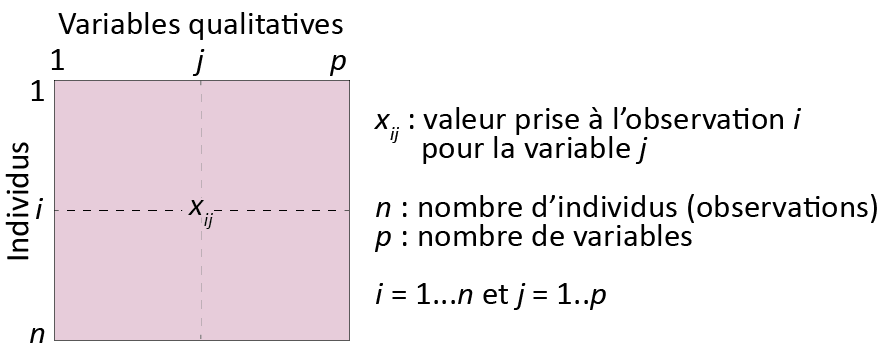
\includegraphics[width=0.6\linewidth]{images/analysesfactorielles/AnalysesFactoriellesTabACM} 

}

\caption{Tableau pour une ACM}\label{fig:AnalysesFactoriellesTabACMFig}
\end{figure}

Par exemple, une enquête sur la mobilité d'une population donnée pourrait comprend plusieurs variables qualitatives dont celles reportées au tableau~\ref{tab:TabACM1}.

\begin{table}

\caption{\label{tab:TabACM1}Exemple de variables qualitatives issues d'une enquête}
\centering
\fontsize{8}{10}\selectfont
\begin{tabular}[t]{lc}
\toprule
Modalités des variables & Codage\\
\midrule
\addlinespace[0.3em]
\multicolumn{2}{l}{\textbf{Sexe}}\\
\hspace{1em}Homme & 1\\
\hspace{1em}Femme & 2\\
\addlinespace[0.3em]
\multicolumn{2}{l}{\textbf{Groupe d'âge}}\\
\hspace{1em}Moins de 20 ans & 1\\
\hspace{1em}20 à 39 ans & 2\\
\hspace{1em}40 à 59 ans & 3\\
\hspace{1em}60 ans et plus & 4\\
\addlinespace[0.3em]
\multicolumn{2}{l}{\textbf{Mode de transport}}\\
\hspace{1em}Automobile & 1\\
\hspace{1em}Transport en commun & 2\\
\hspace{1em}Marche & 3\\
\hspace{1em}Vélo & 4\\
\bottomrule
\end{tabular}
\end{table}

Pour analyser de telles données, il suffit de transformer le tableau condensé (de données brutes) en un tableau disjonctif complet dans lequel chaque modalité des variables qualitatives devient une variable binaire prenant les valeurs de~0 ou~1 (tableaux \ref{tab:TabACM2} et \ref{tab:TabACM3}). Notez que la somme de chaque ligne est alors égale au nombre de variables qualitatives.

\begin{table}

\caption{\label{tab:TabACM2}Tableau condensé (données brutes)}
\centering
\fontsize{8}{10}\selectfont
\begin{tabular}[t]{lccc}
\toprule
  & Sexe & Groupe d'âge & Mode de transport\\
\midrule
Ind. 1 & 1 & 1 & 2\\
Ind. 2 & 1 & 2 & 3\\
Ind. 3 & 2 & 3 & 1\\
Ind. 4 & 1 & 2 & 1\\
Ind. 5 & 2 & 4 & 2\\
\addlinespace
Ind. 6 & 1 & 4 & 4\\
\bottomrule
\end{tabular}
\end{table}

\begin{table}

\caption{\label{tab:TabACM3}Tableau disjonctif complet}
\centering
\fontsize{8}{10}\selectfont
\begin{tabular}[t]{ccccccccccc}
\toprule
\multicolumn{1}{c}{ } & \multicolumn{2}{c}{Sexe} & \multicolumn{4}{c}{Groupe d'âge} & \multicolumn{4}{c}{Mode de transport} \\
\cmidrule(l{3pt}r{3pt}){2-3} \cmidrule(l{3pt}r{3pt}){4-7} \cmidrule(l{3pt}r{3pt}){8-11}
Individu & Homme & Femme & Moins de 20 ans & 20 à 39 ans & 40 à 59 ans & 60 ans et plus & Automobile & Transp. en commun & Marche & Vélo\\
\midrule
Ind. 1 & 1 & 0 & 1 & 0 & 0 & 0 & 0 & 1 & 0 & 0\\
Ind. 2 & 1 & 0 & 0 & 1 & 0 & 0 & 0 & 0 & 1 & 0\\
Ind. 3 & 0 & 1 & 0 & 0 & 1 & 0 & 1 & 0 & 0 & 0\\
Ind. 4 & 1 & 0 & 0 & 1 & 0 & 0 & 1 & 0 & 0 & 0\\
Ind. 5 & 0 & 1 & 0 & 0 & 0 & 1 & 0 & 1 & 0 & 0\\
\addlinespace
Ind. 6 & 1 & 0 & 0 & 0 & 0 & 1 & 0 & 0 & 0 & 1\\
\bottomrule
\end{tabular}
\end{table}

\begin{bloc_astuce}
\textbf{ACM versus AFC}

Nous avons vu que l'AFC permet d'analyser un tableau de contingence avec deux variables qualitatives. En ACM, les colonnes sont alors les différentes modalités des variables qualitatives et les lignes sont les observations (par exemple, les individus ayant répondu à une enquête par sondage). En résumé, l'analyse des correspondances multiples (ACM) est simplement \textbf{une analyse des correspondances (AFC) appliquée sur un tableau disjonctif complet}.

L'ACM permet ainsi de révéler les ressemblances entre les différentes modalités des variables qualitatives et les ressemblances entre les différents individus. Par conséquent, elle produit également des variables synthétiques (axes factoriels) résumant l'information contenue dans le tableau initial. L'évaluation de ces ressemblances et la détermination des axes factoriels sont alors aussi basées sur la \textbf{distance du khi-deux}.

\end{bloc_astuce}

\hypertarget{sect1241}{%
\subsection{Aides à l'interprétation}\label{sect1241}}

Puisque l'ACM est une extension de l'AFC, nous retrouvons les mêmes aides à l'interprétation~: les valeurs propres pour les axes, les coordonnées factorielles, les contributions et les cosinus carrés pour les variables et les individus.

Pour présenter l'ACM, nous utilisons des données ouvertes de la Ville de Montréal et plus particulièrement un \href{https://www.donneesquebec.ca/recherche/dataset/vmtl-agriculture-urbaine-sondage}{sondage auprès de la population de l'île de Montréal sur l'agriculture urbaine}. Pour ce faire, nous avons conservé uniquement les personnes pratiquant l'agriculture urbaine (n~=~352). Les variables qualitatives extraites pour l'ACM sont reportées au tableau~\ref{tab:dataACM} avec la description des questions, leurs modalités respectives avec les effectifs bruts et en pourcentage. Au final, l'ACM est calculée de la manière suivante~:

\begin{itemize}
\tightlist
\item
  Neuf variables qualitatives relatives à la pratique de l'agriculture urbaine sont retenues (\texttt{q3}, \texttt{q4}, \texttt{q5}, \texttt{q8}, \texttt{q9}, \texttt{q10}, \texttt{q11}, \texttt{q12} et \texttt{q13}).
\item
  Quatre variables relatives au profil socioéconomique des personnes répondantes sont introduites comme variables supplémentaires (\texttt{q15}, \texttt{q16}, \texttt{q17}, \texttt{q21}).
\item
  Chaque ligne est pondérée avec la variable \texttt{pond}.
\end{itemize}

L'objectif est de cette ACM double~:

\begin{enumerate}
\def\labelenumi{\arabic{enumi}.}
\tightlist
\item
  Montrer les ressemblances entre les différentes modalités relatives à la pratique de l'agriculture urbaine. L'analyse des axes factoriels devrait nous permettre d'identifier différents profils des personnes pratiquant l'agriculture urbaine.
\item
  Projeter les modalités des variables socioéconomiques afin de vérifier si elles sont ou non associées aux axes factoriels, c'est-à-dire aux différents profils révélés par les axes.
\end{enumerate}

\begin{bloc_attention}
L'analyse du sondage sur l'agriculture urbaine réalisée ici est purement exploratoire~: elle vise uniquement à démonter que l'ACM est un outil particulièrement intéressant pour analyser les données d'un sondage. Par contre, cette analyse n'a aucune prétention scientifique puisque nous ne sommes pas des spécialistes de l'agriculture urbaine. Dans ce champ de recherche très fertile qu'est l'agriculture urbaine (surement pas la meilleure blague du livre\ldots), vous pourrez consulter plusieurs études montréalaises (McClintock \protect\hyperlink{ref-mcclintock2018urban}{2018}; Audate, Cloutier et Lebel \protect\hyperlink{ref-audate2021motivations}{2021}; Bhatt et Farah \protect\hyperlink{ref-bhatt2016cultivating}{2016}).

\end{bloc_attention}

\begin{table}

\caption{\label{tab:dataACM}Variables qualitatives extraites du sondage sur l'agriculture urbaine de la Ville de Montréal}
\centering
\fontsize{8}{10}\selectfont
\begin{tabular}[t]{lrr}
\toprule
Modalité & N & \%\\
\midrule
\addlinespace[0.3em]
\multicolumn{3}{l}{\textbf{Q3.  Depuis combien de temps cultivez-vous des fruits, des fines herbes ou des légumes?}}\\
\hspace{1em}Q3. Moins de 1 an & 35 & 9,9\\
\hspace{1em}Q3. De 1 à 4 ans & 101 & 28,7\\
\hspace{1em}Q3. De 5 à 9 ans & 66 & 18,8\\
\hspace{1em}Q3. 10 ans ou plus & 150 & 42,6\\
\addlinespace[0.3em]
\multicolumn{3}{l}{\textbf{Q4.  Selon vous, quelle proportion des fruits, des fines herbes et des légumes que vous consommez durant l'été provient de votre propre production?}}\\
\hspace{1em}Q4. Moins de 10\% & 192 & 54,5\\
\hspace{1em}Q4. 10 à 25\% & 70 & 19,9\\
\hspace{1em}Q4. 26 à 50\% & 47 & 13,4\\
\hspace{1em}Q4. Plus de 50\% & 43 & 12,2\\
\addlinespace[0.3em]
\multicolumn{3}{l}{\textbf{Q5.  Utilisez-vous du compost provenant de vos déchets verts ou de vos déchets alimentaires pour faire pousser des fruits, des fines herbes ou des légumes?}}\\
\hspace{1em}Q5. Oui & 90 & 25,6\\
\hspace{1em}Q5. Non & 262 & 74,4\\
\addlinespace[0.3em]
\multicolumn{3}{l}{\textbf{Q8.  Récupérez-vous l'eau de pluie pour irriguer vos cultures de fruits, de fines herbes ou des légumes ou encore votre jardin?}}\\
\hspace{1em}Q8. Oui & 72 & 20,5\\
\hspace{1em}Q8. Non & 280 & 79,5\\
\addlinespace[0.3em]
\multicolumn{3}{l}{\textbf{Q9.  Combien de sortes de fruits, de fines herbes ou des légumes cultivez-vous?}}\\
\hspace{1em}Q9. Moins de 5 sortes & 170 & 48,3\\
\hspace{1em}Q9. 5 à 9 sortes & 124 & 35,2\\
\hspace{1em}Q9. 10 à 14 sortes & 42 & 11,9\\
\hspace{1em}Q9. 15 sortes ou plus & 16 & 4,5\\
\addlinespace[0.3em]
\multicolumn{3}{l}{\textbf{Q10. Cultivez-vous suffisamment de fruits, de fines herbes ou des légumes pour partager avec d'autres personnes?}}\\
\hspace{1em}Q10. Oui & 143 & 40,6\\
\hspace{1em}Q10. Non & 209 & 59,4\\
\addlinespace[0.3em]
\multicolumn{3}{l}{\textbf{Q11. Échangez-vous vos semis ou vos récoltes de fruits, de fines herbes ou des légumes avec d'autres personnes?}}\\
\hspace{1em}Q11. Oui & 90 & 25,6\\
\hspace{1em}Q11. Non & 262 & 74,4\\
\addlinespace[0.3em]
\multicolumn{3}{l}{\textbf{Q12. Selon vous, l'agriculture urbaine contribue-t-elle à améliorer les rapports entre les gens?}}\\
\hspace{1em}Q12. Oui & 283 & 80,4\\
\hspace{1em}Q12. Non & 46 & 13,1\\
\hspace{1em}Q12. NSP/NRP & 23 & 6,5\\
\addlinespace[0.3em]
\multicolumn{3}{l}{\textbf{Q13. Saviez-vous que la Ville de Montréal encourage et soutient l'agriculture urbaine sur l'île de Montréal?}}\\
\hspace{1em}Q13. Oui & 203 & 57,7\\
\hspace{1em}Q13. Non & 149 & 42,3\\
\addlinespace[0.3em]
\multicolumn{3}{l}{\textbf{Q15. À quel groupe d'âge appartenez-vous?}}\\
\hspace{1em}Q15. 18 à 34 ans & 54 & 15,3\\
\hspace{1em}Q15. 35 à 49 ans & 110 & 31,2\\
\hspace{1em}Q15. 50 à 64 ans & 101 & 28,7\\
\hspace{1em}Q15. 65 ans et plus & 87 & 24,7\\
\addlinespace[0.3em]
\multicolumn{3}{l}{\textbf{Q16. Quelle est votre occupation principale?}}\\
\hspace{1em}Q16. Travail temps plein & 177 & 50,3\\
\hspace{1em}Q16. Travail. temps partiel & 26 & 7,4\\
\hspace{1em}Q16. Étudiant & 14 & 4,0\\
\hspace{1em}Q16. Retraité & 101 & 28,7\\
\hspace{1em}Q16. Sans emploi & 10 & 2,8\\
\hspace{1em}Q16. À la maison & 24 & 6,8\\
\addlinespace[0.3em]
\multicolumn{3}{l}{\textbf{Q17. Quel est le plus haut niveau de scolarité que vous avez complété?}}\\
\hspace{1em}Q17. Aucun certificat ou dipl. & 25 & 7,1\\
\hspace{1em}Q17. Dipl. secondaires & 80 & 22,7\\
\hspace{1em}Q17. Dipl. collégiales & 75 & 21,3\\
\hspace{1em}Q17. Études universitaires & 172 & 48,9\\
\addlinespace[0.3em]
\multicolumn{3}{l}{\textbf{Q21. Êtes-vous propriétaire ou locataire de votre résidence ?}}\\
\hspace{1em}Q17. Refus & 0 & 0,0\\
\hspace{1em}Q21. Propriétaire & 250 & 71,0\\
Q22. Locataire & 102 & 29,0\\
\bottomrule
\end{tabular}
\end{table}

\hypertarget{sect12411}{%
\subsubsection{Résultats de l'ACM pour les valeurs propres}\label{sect12411}}

Les résultats pour les valeurs propres sont reportés au tableau~\ref{tab:ACMValeursPropresTab} et à la figure~\ref{fig:ACMValeursPropresFig}.
En ACM, l'inertie totale du tableau des variables qualitatives est égale au nombre moyen de modalités par variable moins un, soit \(\frac{K}{J}-1\) avec \emph{K} et \emph{J} étant respectivement les nombres de modalités et de variables. Aussi, le nombre d'axes produits par l'ACM est égal à \(K - J\). Pour notre tableau, l'inertie est donc égale à \(\mbox{25} / \mbox{9} = \mbox{1,77}\) avec 16 avec \(\mbox{25}-\mbox{9} = \mbox{16}\) axes. Le nombre d'axes à retenir est souvent plus difficile à déterminer puisque tel que signalé judicieusement par Jérôme Pagès (\protect\hyperlink{ref-pages2002analyse}{2002}, pp.~53) : «~en pratique, comparée à l'ACP, l'ACM conduit, dans l'ensemble à~: des pourcentages d'inertie plus petits; une décroissance de ces pourcentages plus douce~».

L'histogramme des valeurs propres (figure~\ref{fig:ACMValeursPropresFig}) révèle plusieurs sauts importants dans les valeurs propres qui pourraient justifier le choix du nombre d'axes factoriels, soit aux axes~1, 2, 3 et~6. Pour l'exercice, nous retenons les trois premiers axes qui résument 30~\% de l'inertie du tableau initial.

\begin{table}

\caption{\label{tab:ACMValeursPropresTab}Résultats de l'ACM pour les valeurs propres}
\centering
\fontsize{8}{10}\selectfont
\begin{tabular}[t]{rrrr}
\toprule
Axe factoriel & Valeur propre & Pourcentage & Pourc. cumulé\\
\midrule
1 & 0,248 & 13,940 & 13,940\\
2 & 0,156 & 8,792 & 22,732\\
3 & 0,135 & 7,620 & 30,352\\
4 & 0,127 & 7,161 & 37,513\\
5 & 0,126 & 7,065 & 44,579\\
\addlinespace
6 & 0,123 & 6,916 & 51,494\\
7 & 0,114 & 6,385 & 57,879\\
8 & 0,107 & 6,003 & 63,882\\
9 & 0,101 & 5,671 & 69,553\\
10 & 0,095 & 5,327 & 74,880\\
\addlinespace
11 & 0,093 & 5,234 & 80,115\\
12 & 0,086 & 4,822 & 84,937\\
13 & 0,077 & 4,340 & 89,277\\
14 & 0,071 & 4,011 & 93,288\\
15 & 0,064 & 3,619 & 96,906\\
\addlinespace
16 & 0,055 & 3,094 & 100,000\\
\bottomrule
\end{tabular}
\end{table}

\begin{figure}

{\centering \includegraphics[width=0.75\linewidth]{livre_statistique_Phil_Jere_clean_files/figure-latex/ACMValeursPropresFig-1} 

}

\caption{Graphiques pour les valeurs propres pour l'ACM}\label{fig:ACMValeursPropresFig}
\end{figure}

\hypertarget{sect12412}{%
\subsubsection{Résultats de l'ACM pour les modalités des variables}\label{sect12412}}

À titre de rappel, comme pour l'ACP et l'AFC, nous retrouvons les trois mêmes mesures pour les variables et les individus~ (coordonnées factorielles, contributions et cosinus carrés). Plus les variables qualitatives du jeu données comprennent de modalités, plus la taille du tableau des résultats des modalités sera importante et plus il est fastidieux de l'analyser. Il est donc recommandé de construire des histogrammes avec les coordonnées factorielles et les contributions des modalités, mais aussi un nuage de points avec les coordonnées des variables sur le premier plan factoriel voire le deuxième.

\begin{bloc_objectif}
\textbf{Compréhension des axes factoriels de l'ACM~: une étape essentielle, incontournable\ldots{}}

Comme en ACP et en AFC, l'analyse des trois mesures (coordonnées, contributions et cosinus carrés) pour les variables et les individus doit vous permettre de comprendre la signification des axes factoriels retenus de l'ACM. Prenez le temps de bien réaliser cette étape d'interprétation souvent plus fastidieuse qu'en ACP et ACM, en raison du nombre élevé de modalités. Cette étape est en effet essentielle afin de qualifier les variables latentes (axes factoriels, variables synthétiques) produites par l'ACM.

\end{bloc_objectif}

Les résultats pour les variables sont reportés 1) au tableau~\ref{tab:ACMValeursCoordTab}, 2) aux figure~\ref{fig:ACMValeursCoordFig1}, \ref{fig:ACMValeursCoordFig2} et \ref{fig:ACMValeursCoordFig3} pour les coordonnées et les contributions et à la figure~\ref{fig:ACMValeursPlanFacto1} pour le premier plan factoriel.

\textbf{Interprétation des résultats de l'axe~1 pour les variables}

Sept modalités concourent le plus à la formation de l'axe~1 résumant 13,9~\% de la variance~: \texttt{Q9.\ 10\ à\ 14\ sortes} (10,35~\%), \texttt{Q10.\ Oui} (9,99~\%), \texttt{Q9.\ Moins\ de\ 5\ sortes} (9,71~\%), \texttt{Q5.\ Oui} (9,19~\%), \texttt{Q11.\ Oui} (8,20~\%), \texttt{Q4.\ Moins\ de\ 10\%} (7,87~\%) et \texttt{Q10.\ Non} (7,10~\%). Aussi, les modalités suivantes sont présentes aux deux extrémités de cet axe~:

\begin{itemize}
\tightlist
\item
  \textbf{Coordonnées négatives}~: \texttt{Q12.\ Non} (-0,84), \texttt{Q3.\ Moins\ de\ 1\ an} (-0,73), \texttt{Q9.\ Moins\ de\ 5\ sortes} (-0,67), \texttt{Q4.\ Moins\ de\ 10\%} (-0,56), \texttt{Q10.\ Non} (-0,521). Cela signifie que lorsque les coordonnées des individus sont fortement négatives sur cet axe, les personnes pratiquant l'agriculture urbaine~:

  \begin{itemize}
  \tightlist
  \item
    \emph{ne pensent pas que l'agriculture urbaine contribue à améliorer les rapports entre les gens} (\texttt{Q12});
  \item
    \emph{cultivent des fruits, des fines herbes ou des légumes depuis moins d'un an} (\texttt{Q3});
  \item
    \emph{cultivent moins de cinq sortes de fruits, de fines herbes ou de légumes} (\texttt{Q9});
  \item
    \emph{moins de 10~\% de leur proportion des fruits, des fines herbes et des légumes consommés durant l'été provient de votre propre production }(\texttt{Q4});
  \item
    \emph{ne cultivent pas suffisamment pour partager avec d'autres personnes} (\texttt{Q10}).
  \end{itemize}
\item
  \textbf{Coordonnées positives}~: \texttt{Q9.\ 15\ sortes\ ou\ plus} (1,36), \texttt{Q9.\ 10\ à\ 14\ sortes} (1,28), \texttt{Q5.\ Oui} (0,95) et \texttt{Q11.\ Oui} (0,85). Cela signifie que lorsque les coordonnées des individus sont fortement positives sur cet axe, les personnes pratiquant l'agriculture urbaine~:

  \begin{itemize}
  \tightlist
  \item
    \emph{cultivent plus de dix sortes de fruits, de fines herbes ou de légumes} (\texttt{Q9});
  \item
    \emph{utilisent du compost provenant de leurs déchets verts ou de leurs déchets alimentaires pour faire pousser des fruits, des fines herbes ou des légumes} (\texttt{Q5});
  \item
    \emph{échangent leurs semis ou leurs récoltes de fruits, de fines herbes ou des légumes avec d'autres personnes} (\texttt{Q11}).
  \end{itemize}
\end{itemize}

En résumé, l'axe~1 oppose clairement les \textbf{«~néophytes en agriculture~»} versus les \textbf{personnes expérimentées} cultivant des fruits et légumes variés avec leur propre compost et échangeant leurs semis ou récoltes.

\begin{table}

\caption{\label{tab:ACMValeursCoordTab}Résultats de l'ACM pour les modalités des variables}
\centering
\fontsize{8}{10}\selectfont
\begin{tabular}[t]{lrrrrrrrrr}
\toprule
\multicolumn{1}{c}{ } & \multicolumn{3}{c}{Coordonnées} & \multicolumn{3}{c}{Cosinus carrés} & \multicolumn{3}{c}{Contributions (\%)} \\
\cmidrule(l{3pt}r{3pt}){2-4} \cmidrule(l{3pt}r{3pt}){5-7} \cmidrule(l{3pt}r{3pt}){8-10}
Modalité & 1 & 2 & 3 & 1 & 2 & 3 & 1 & 2 & 3\\
\midrule
Q3. Moins de 1 an & -0,73 & 0,68 & 0,63 & 2,70 & 3,68 & 3,64 & 0,07 & 0,06 & 0,05\\
Q3. De 1 à 4 ans & -0,29 & -0,79 & 0,39 & 1,26 & 15,30 & 4,30 & 0,04 & 0,33 & 0,08\\
Q3. De 5 à 9 ans & 0,12 & 0,38 & -1,11 & 0,12 & 2,02 & 19,43 & 0,00 & 0,04 & 0,29\\
Q3. 10 ans ou plus & 0,45 & 0,35 & 0,02 & 3,19 & 3,01 & 0,02 & 0,11 & 0,07 & 0,00\\
Q4. Moins de 10\% & -0,56 & 0,03 & 0,07 & 7,87 & 0,04 & 0,22 & 0,40 & 0,00 & 0,01\\
\addlinespace
Q4. 10 à 25\% & 0,74 & -0,76 & -0,11 & 4,92 & 8,22 & 0,19 & 0,14 & 0,14 & 0,00\\
Q4. 26 à 50\% & 0,78 & 0,64 & 0,15 & 3,82 & 4,18 & 0,28 & 0,10 & 0,07 & 0,00\\
Q4. Plus de 50\% & 0,53 & 0,40 & -0,37 & 1,31 & 1,17 & 1,19 & 0,03 & 0,02 & 0,02\\
Q5. Oui & 0,95 & 0,56 & -0,13 & 9,19 & 5,01 & 0,29 & 0,27 & 0,09 & 0,00\\
Q5. Non & -0,28 & -0,16 & 0,04 & 2,70 & 1,47 & 0,09 & 0,27 & 0,09 & 0,00\\
\addlinespace
Q8. Oui & 0,55 & 0,37 & 1,21 & 2,58 & 1,86 & 23,31 & 0,07 & 0,03 & 0,35\\
Q8. Non & -0,13 & -0,09 & -0,29 & 0,62 & 0,45 & 5,60 & 0,07 & 0,03 & 0,35\\
Q9. Moins de 5 sortes & -0,67 & 0,01 & 0,47 & 9,71 & 0,00 & 8,83 & 0,42 & 0,00 & 0,21\\
Q9. 5 à 9 sortes & 0,24 & 0,11 & -0,79 & 0,89 & 0,30 & 17,31 & 0,03 & 0,01 & 0,32\\
Q9. 10 à 14 sortes & 1,28 & -0,97 & 0,07 & 10,35 & 9,42 & 0,06 & 0,27 & 0,15 & 0,00\\
\addlinespace
Q9. 15 sortes ou plus & 1,36 & 2,15 & 0,65 & 3,62 & 14,42 & 1,50 & 0,08 & 0,21 & 0,02\\
Q10. Oui & 0,73 & -0,15 & 0,07 & 9,99 & 0,63 & 0,18 & 0,38 & 0,02 & 0,00\\
Q10. Non & -0,52 & 0,10 & -0,05 & 7,10 & 0,45 & 0,13 & 0,38 & 0,02 & 0,00\\
Q11. Oui & 0,85 & -0,83 & 0,32 & 8,20 & 12,45 & 2,11 & 0,25 & 0,23 & 0,03\\
Q11. Non & -0,29 & 0,28 & -0,11 & 2,79 & 4,24 & 0,72 & 0,25 & 0,23 & 0,03\\
\addlinespace
Q12. Oui & 0,16 & 0,02 & 0,01 & 0,97 & 0,02 & 0,01 & 0,11 & 0,00 & 0,00\\
Q12. Non & -0,84 & -0,38 & 0,09 & 4,12 & 1,32 & 0,08 & 0,11 & 0,02 & 0,00\\
Q12. NSP/NRP & -0,36 & 0,56 & -0,31 & 0,36 & 1,39 & 0,48 & 0,01 & 0,02 & 0,01\\
Q13. Oui & 0,17 & 0,31 & 0,31 & 0,70 & 3,91 & 4,37 & 0,04 & 0,13 & 0,12\\
Q13. Non & -0,22 & -0,40 & -0,40 & 0,91 & 5,05 & 5,66 & 0,04 & 0,13 & 0,12\\
\bottomrule
\end{tabular}
\end{table}

\begin{figure}

{\centering \includegraphics[width=1\linewidth]{livre_statistique_Phil_Jere_clean_files/figure-latex/ACMValeursCoordFig1-1} 

}

\caption{Graphiques pour les résultats des modalités de l'axe 1 de l'ACM}\label{fig:ACMValeursCoordFig1}
\end{figure}

\textbf{Interprétation des résultats de l'axe~2 pour les variables}

Quatre modalités concourent le plus à la formation de l'axe~1 résumant 8,8~\% de la variance~: \texttt{Q3.\ De\ 1\ à\ 4\ ans} (15,30~\%), \texttt{Q9.\ 15\ sortes\ ou\ plus} (14,42~\%), \texttt{Q11.\ Oui} (12,45~\%) et \texttt{Q9.\ 10\ à\ 14\ sortes} (9,42~\%). Les modalités suivantes sont présentes aux deux extrémités de l'axe~2~:

\begin{itemize}
\tightlist
\item
  \textbf{Coordonnées négatives}~: \texttt{Q9.\ 10\ à\ 14\ sortes} (-0,97), \texttt{Q11.\ Oui} (-0,83), \texttt{Q3.\ De\ 1\ à\ 4\ ans} (-0,79), \texttt{Q4.\ 10\ à\ 25\%} (-0,76). Cela signifie que lorsque les coordonnées des individus sont fortement négatives sur cet axe, les personnes pratiquant l'agriculture urbaine~:

  \begin{itemize}
  \tightlist
  \item
    \emph{cultivent de 10 à 14 sortes de fruits, de fines herbes ou de légumes} (\texttt{Q9});
  \item
    \emph{échangent leurs semis ou leurs récoltes de fruits, de fines herbes ou des légumes avec d'autres personnes} (\texttt{Q11});
  \item
    \emph{cultivent des fruits, des fines herbes ou des légumes depuis 1 à 4 ans} (\texttt{Q3});
  \item
    \emph{de 10 à 25~\% de leur proportion des fruits, des fines herbes et des légumes consommés durant l'été provient de votre propre production }(\texttt{Q4}).
  \end{itemize}
\item
  \textbf{Coordonnées positives}~: seule la modalité \texttt{Q9.\ 15\ sortes\ ou\ plus} (2,15) présente une forte coordonnée positive.
\end{itemize}

\textbf{En résumé, l'axe~2} permet surtout d'identifier des personnes pratiquant l'agriculture urbaine depuis quelques années (de 1 à 4 ans), mais cultivant déjà nombreuses sortent de fruits et légumes et partageant aussi leurs semis ou récoltes.

\begin{figure}

{\centering \includegraphics[width=1\linewidth]{livre_statistique_Phil_Jere_clean_files/figure-latex/ACMValeursCoordFig2-1} 

}

\caption{Graphiques pour les résultats des modalités de l'axe 2 de l'ACM}\label{fig:ACMValeursCoordFig2}
\end{figure}

\begin{figure}

{\centering \includegraphics[width=0.75\linewidth]{livre_statistique_Phil_Jere_clean_files/figure-latex/ACMValeursPlanFacto1-1} 

}

\caption{Premier plan factoriel de l'ACM pour les modalités}\label{fig:ACMValeursPlanFacto1}
\end{figure}

\textbf{Interprétation des résultats de l'axe~3 pour les variables}

Trois modalités concourent le plus à la formation de l'axe~3 résumant 7,6~\% de la variance~: \texttt{Q8.\ Oui} (23,31), \texttt{Q3.\ De\ 5\ à\ 9\ ans} (19,43) et \texttt{Q9.\ 5\ à\ 9\ sortes} (17,31). Les modalités suivantes sont présentes aux deux extrémités de l'axe~3~:

\begin{itemize}
\tightlist
\item
  \textbf{Coordonnées négatives}~: \texttt{Q3.\ De\ 5\ à\ 9\ ans} (-1,11), \texttt{Q9.\ 5\ à\ 9\ sortes} (-0,79).
\item
  \textbf{Coordonnées positives}~: seule la modalité \texttt{Q8.\ Oui} présente une coordonnée fortement positive (1,21).
\end{itemize}

Par conséquent, cet axe semble plus complexe à analyser et surtout moins intéressant que les deux premiers.

\begin{figure}

{\centering \includegraphics[width=1\linewidth]{livre_statistique_Phil_Jere_clean_files/figure-latex/ACMValeursCoordFig3-1} 

}

\caption{Graphiques pour les résultats des modalités de l'axe 3 de l'ACM}\label{fig:ACMValeursCoordFig3}
\end{figure}

\textbf{Introduction des variables supplémentaires}

Il est ensuite possible de projeter les modalités supplémentaires sur les axes de l'ACM retenus (tableau~\ref{tab:ACMValeursCoordSupplTab} et figure~\ref{fig:ACMValeursPlanFactoSupp1}). Les faibles valeurs des coordonnées factorielles des modalités supplémentaires sur les deux axes semblent indiquer que le profil socioéconomique des personnes pratiquant l'agriculture urbaine ne semble pas (ou peu) relié aux profils identifiés par les axes factoriels.

\begin{table}

\caption{\label{tab:ACMValeursCoordSupplTab}Résultats de l'ACM pour les modalités des variables supplémentaires}
\centering
\fontsize{8}{10}\selectfont
\begin{tabular}[t]{lrrrr}
\toprule
\multicolumn{1}{c}{ } & \multicolumn{2}{c}{Coordonnées} & \multicolumn{2}{c}{Cosinus carrés} \\
\cmidrule(l{3pt}r{3pt}){2-3} \cmidrule(l{3pt}r{3pt}){4-5}
Modalité & 1 & 2 & 1 & 2\\
\midrule
Q15. 18 à 34 ans & -0,09 & -0,27 & 0,00 & 0,04\\
Q15. 35 à 49 ans & -0,06 & -0,01 & 0,00 & 0,00\\
Q15. 50 à 64 ans & 0,14 & 0,25 & 0,01 & 0,02\\
Q15. 65 ans et plus & 0,11 & 0,25 & 0,00 & 0,01\\
Q16. Travail temps plein & -0,10 & -0,06 & 0,01 & 0,01\\
\addlinespace
Q16. Travail. temps partiel & 0,36 & -0,15 & 0,01 & 0,00\\
Q16. Étudiant & -0,14 & -0,11 & 0,00 & 0,00\\
Q16. Retraité & 0,17 & 0,25 & 0,01 & 0,02\\
Q16. Sans emploi & 0,44 & -0,14 & 0,01 & 0,00\\
Q16. À la maison & -0,06 & 0,18 & 0,00 & 0,00\\
\addlinespace
Q17. Aucun certificat ou dipl. & 0,28 & 0,16 & 0,00 & 0,00\\
Q17. Dipl. secondaires & -0,09 & 0,01 & 0,00 & 0,00\\
Q17. Dipl. collégiales & 0,01 & 0,19 & 0,00 & 0,01\\
Q17. Études universitaires & 0,00 & -0,10 & 0,00 & 0,01\\
Q21. Propriétaire & 0,03 & 0,02 & 0,00 & 0,00\\
\addlinespace
Q22. Locataire & -0,06 & -0,03 & 0,00 & 0,00\\
\bottomrule
\end{tabular}
\end{table}

\begin{verbatim}
## Warning: ggrepel: 12 unlabeled data points (too many overlaps). Consider
## increasing max.overlaps
\end{verbatim}

\begin{figure}

{\centering \includegraphics[width=1\linewidth]{livre_statistique_Phil_Jere_clean_files/figure-latex/ACMValeursPlanFactoSupp1-1} 

}

\caption{Premier plan factoriel de l'ACM avec toutes les modalités incluant celles supplémentaires}\label{fig:ACMValeursPlanFactoSupp1}
\end{figure}

\begin{bloc_astuce}

\textbf{Visualisation de variables qualitatives ordinales sur un plan factoriel}

Lorsque les variables qualitatives sont ordinales et non nominales, il peut être intéressant de relier les différentes modalités avec une ligne. Cela permet de comprendre en un coup d'œil la trajectoire que suivent les modalités sur les deux axes factoriels. En guise d'exemple, nous réalisons cet exercice pour les variables \texttt{Q3} et \texttt{Q9} (figure~\ref{fig:ACMordinaleTrajectoire}).

\begin{figure}

{\centering \includegraphics[width=1\linewidth]{livre_statistique_Phil_Jere_clean_files/figure-latex/ACMordinaleTrajectoire-1} 

}

\caption{Trajectoires des variables ordinales sur le premier plan factoriel de l'ACM }\label{fig:ACMordinaleTrajectoire}
\end{figure}


\end{bloc_astuce}

\hypertarget{sect12413}{%
\subsubsection{Résultats de l'ACM pour les individus}\label{sect12413}}

Comme toute méthode factorielle, les coordonnées factorielles, les cosinus carrés et les contributions sont aussi disponibles pour les individus. Nous proposons ici simplement de réaliser le premier plan factoriel pour les individus en attribuant un dégradé de couleurs avec les cosinus carrés (figure~\ref{fig:ACMValeursPlanFactoSupp1}). Il est aussi possible d'attribuer des couleurs aux différentes modalités d'une variable. Par exemple, sur le premier plan factoriel, nous avons utilisé la variable \texttt{Q12.\ Selon\ vous,\ l’agriculture\ urbaine\ contribue-t-elle\ à\ améliorer\ les\ rapports\ entre\ les\ gens?}. Cela permet de repérer visuellement que les personnes ayant répondu non à cette question ont surtout coordonnées négatives sur l'axe~1.

\begin{figure}

{\centering \includegraphics[width=1\linewidth]{livre_statistique_Phil_Jere_clean_files/figure-latex/ACMPlanFacto12Ind1-1} 

}

\caption{Premier plan factoriel de l'ACM pour les individus}\label{fig:ACMPlanFacto12Ind1}
\end{figure}

\begin{figure}

{\centering \includegraphics[width=1\linewidth]{livre_statistique_Phil_Jere_clean_files/figure-latex/ACMPlanFacto12Ind2-1} 

}

\caption{Premier plan factoriel de l'ACM pour les individus avec coloration d'une variable}\label{fig:ACMPlanFacto12Ind2}
\end{figure}

\hypertarget{sect1242}{%
\subsection{Mise en œuvre dans R}\label{sect1242}}

\hypertarget{sect12421}{%
\subsubsection{\texorpdfstring{Calcul d'une ACM avec \texttt{FactoMineR}}{Calcul d'une ACM avec FactoMineR}}\label{sect12421}}

Plusieurs \emph{packages} permettent de calculer une ACM dans R, notamment \texttt{ExPosition} (fonction \texttt{epMCA}), \texttt{ade4} (fonction \texttt{dudi.mca}) et \texttt{FactoMineR} (fonction \texttt{MCA}). De nouveau, nous utilisons \texttt{FactoMineR} couplé au \emph{package} \texttt{factoextra} pour réaliser rapidement des graphiques.

Pour calculer l'ACM, il suffit d'utiliser la fonction \texttt{MCA} de \texttt{FactoMineR}, puis la fonction \texttt{summary(res.acm)} qui renvoie les résultats de l'AFC pour~:

\begin{itemize}
\tightlist
\item
  Les valeurs propres (section \texttt{Eigenvalues}) pour les axes factoriels (\texttt{Dim.1} à \texttt{Dim.n}) avec leur variance expliquée brute (\texttt{Variance}), en pourcentage (\texttt{\%\ of\ var.}) et en pourcentage cumulé (\texttt{Cumulative\ \%\ of\ var.}).
\item
  Les dix premières observations (section \texttt{Rows}) avec les coordonnées factorielles (\texttt{Dim.1} à \texttt{Dim.n}), les contributions (\texttt{ctr}) et les cosinus carrés (\texttt{cos2}). Pour accéder aux résultats pour toutes les observations, utilisez les fonctions \texttt{res.acm\$row} ou encore \texttt{res.acm\$row\$coord} (uniquement les coordonnées factorielles), \texttt{res.acm\$row\$contrib} (uniquement les contributions) et \texttt{res.acm\$ind\$cos2} (uniquement les cosinus carrés).
\item
  Les dix premières modalités des variables (section \texttt{Categories}) avec les coordonnées factorielles (D\texttt{im.1} à \texttt{Dim.n}), les contributions (\texttt{ctr}) et les cosinus carrés (\texttt{cos2}).
\end{itemize}

La syntaxe ci-dessous permet dans un premier temps de calculer l'ACM, puis de créer un \emph{dataframe} pour les résultats des valeurs propres.

\begin{Shaded}
\begin{Highlighting}[]
\KeywordTok{library}\NormalTok{(FactoMineR)}
\CommentTok{# Calcul de l'AFC}
\NormalTok{res.acm <-}\StringTok{  }\KeywordTok{MCA}\NormalTok{(dfACM,            }\CommentTok{# Nom du dataframe}
                \DataTypeTok{ncp =} \DecValTok{3}\NormalTok{,          }\CommentTok{# Nombre d'axes retenus}
                \DataTypeTok{quali.sup=}\DecValTok{10}\OperatorTok{:}\DecValTok{13}\NormalTok{,  }\CommentTok{# Variables supplémentaires}
                \DataTypeTok{graph =} \OtherTok{FALSE}\NormalTok{, }
                \DataTypeTok{row.w =}\NormalTok{ dfenquete}\OperatorTok{$}\NormalTok{pond) }\CommentTok{# Variables pour la pondération des lignes}
\CommentTok{# Affichage des résultats}
\KeywordTok{print}\NormalTok{(res.acm)}
\end{Highlighting}
\end{Shaded}

\begin{verbatim}
## **Results of the Multiple Correspondence Analysis (MCA)**
## The analysis was performed on 352 individuals, described by 13 variables
## *The results are available in the following objects:
## 
##    name                description                                          
## 1  "$eig"              "eigenvalues"                                        
## 2  "$var"              "results for the variables"                          
## 3  "$var$coord"        "coord. of the categories"                           
## 4  "$var$cos2"         "cos2 for the categories"                            
## 5  "$var$contrib"      "contributions of the categories"                    
## 6  "$var$v.test"       "v-test for the categories"                          
## 7  "$ind"              "results for the individuals"                        
## 8  "$ind$coord"        "coord. for the individuals"                         
## 9  "$ind$cos2"         "cos2 for the individuals"                           
## 10 "$ind$contrib"      "contributions of the individuals"                   
## 11 "$quali.sup"        "results for the supplementary categorical variables"
## 12 "$quali.sup$coord"  "coord. for the supplementary categories"            
## 13 "$quali.sup$cos2"   "cos2 for the supplementary categories"              
## 14 "$quali.sup$v.test" "v-test for the supplementary categories"            
## 15 "$call"             "intermediate results"                               
## 16 "$call$marge.col"   "weights of columns"                                 
## 17 "$call$marge.li"    "weights of rows"
\end{verbatim}

\begin{Shaded}
\begin{Highlighting}[]
\KeywordTok{summary}\NormalTok{(res.acm)}
\end{Highlighting}
\end{Shaded}

\begin{verbatim}
## 
## Call:
## MCA(X = dfACM, ncp = 3, quali.sup = 10:13, graph = FALSE, row.w = dfenquete$pond) 
## 
## 
## Eigenvalues
##                        Dim.1   Dim.2   Dim.3   Dim.4   Dim.5   Dim.6   Dim.7
## Variance               0.248   0.156   0.135   0.127   0.126   0.123   0.114
## % of var.             13.940   8.792   7.620   7.161   7.065   6.916   6.385
## Cumulative % of var.  13.940  22.732  30.352  37.513  44.579  51.494  57.879
##                        Dim.8   Dim.9  Dim.10  Dim.11  Dim.12  Dim.13  Dim.14
## Variance               0.107   0.101   0.095   0.093   0.086   0.077   0.071
## % of var.              6.003   5.671   5.327   5.234   4.822   4.340   4.011
## Cumulative % of var.  63.882  69.553  74.880  80.115  84.937  89.277  93.288
##                       Dim.15  Dim.16
## Variance               0.064   0.055
## % of var.              3.619   3.094
## Cumulative % of var.  96.906 100.000
## 
## Individuals (the 10 first)
##                                Dim.1    ctr   cos2    Dim.2    ctr   cos2  
## 4                           |  0.261  0.063  0.052 |  0.327  0.155  0.081 |
## 10                          | -0.533  0.688  0.278 |  0.050  0.010  0.002 |
## 11                          |  0.135  0.020  0.014 | -0.120  0.025  0.011 |
## 15                          |  0.020  0.000  0.000 |  0.271  0.073  0.061 |
## 17                          | -0.133  0.014  0.012 | -0.264  0.088  0.049 |
## 18                          |  0.196  0.024  0.018 |  0.279  0.078  0.037 |
## 19                          | -0.193  0.041  0.014 | -0.063  0.007  0.002 |
## 21                          |  0.845  0.731  0.369 | -0.337  0.184  0.059 |
## 23                          | -0.253  0.155  0.058 | -0.020  0.002  0.000 |
## 26                          |  0.802  0.552  0.170 |  0.460  0.288  0.056 |
##                              Dim.3    ctr   cos2  
## 4                            0.251  0.105  0.048 |
## 10                          -0.413  0.757  0.167 |
## 11                          -0.354  0.252  0.097 |
## 15                          -0.503  0.291  0.209 |
## 17                           0.835  1.019  0.486 |
## 18                           0.104  0.012  0.005 |
## 19                           0.159  0.051  0.010 |
## 21                          -0.390  0.285  0.079 |
## 23                          -0.375  0.624  0.128 |
## 26                           0.098  0.015  0.003 |
## 
## Categories (the 10 first)
##                                 Dim.1     ctr    cos2  v.test     Dim.2     ctr
## Q3. Moins de 1 an           |  -0.731   2.704   0.068  -4.940 |   0.677   3.681
## Q3. De 1 à 4 ans            |  -0.286   1.259   0.043  -3.921 |  -0.791  15.299
## Q3. De 5 à 9 ans            |   0.119   0.122   0.003   1.102 |   0.385   2.023
## Q3. 10 ans ou plus          |   0.450   3.189   0.110   6.271 |   0.347   3.006
## Q4. Moins de 10%            |  -0.562   7.874   0.395 -11.913 |   0.033   0.044
## Q4. 10 à 25%                |   0.745   4.918   0.137   7.006 |  -0.765   8.220
## Q4. 26 à 50%                |   0.775   3.815   0.099   5.966 |   0.644   4.176
## Q4. Plus de 50%             |   0.527   1.310   0.033   3.424 |   0.395   1.167
## Q5. Oui                     |   0.950   9.194   0.265   9.760 |   0.557   5.008
## Q5. Non                     |  -0.279   2.701   0.265  -9.760 |  -0.164   1.471
##                                cos2  v.test     Dim.3     ctr    cos2  v.test  
## Q3. Moins de 1 an             0.058   4.578 |   0.627   3.636   0.050   4.236 |
## Q3. De 1 à 4 ans              0.328 -10.855 |   0.390   4.304   0.080   5.360 |
## Q3. De 5 à 9 ans              0.035   3.556 |  -1.110  19.427   0.293 -10.261 |
## Q3. 10 ans ou plus            0.065   4.835 |   0.023   0.016   0.000   0.327 |
## Q4. Moins de 10%              0.001   0.704 |   0.070   0.221   0.006   1.477 |
## Q4. 10 à 25%                  0.144  -7.194 |  -0.109   0.191   0.003  -1.021 |
## Q4. 26 à 50%                  0.068   4.957 |   0.154   0.276   0.004   1.187 |
## Q4. Plus de 50%               0.018   2.566 |  -0.372   1.195   0.016  -2.417 |
## Q5. Oui                       0.091   5.720 |  -0.126   0.294   0.005  -1.290 |
## Q5. Non                       0.091  -5.720 |   0.037   0.086   0.005   1.290 |
## 
## Categorical variables (eta2)
##                               Dim.1 Dim.2 Dim.3  
## q3                          | 0.162 0.338 0.334 |
## q4                          | 0.400 0.191 0.023 |
## q5                          | 0.265 0.091 0.005 |
## q8                          | 0.071 0.032 0.352 |
## q9                          | 0.548 0.340 0.338 |
## q10                         | 0.381 0.015 0.004 |
## q11                         | 0.245 0.235 0.034 |
## q12                         | 0.121 0.038 0.007 |
## q13                         | 0.036 0.126 0.122 |
## 
## Supplementary categories (the 10 first)
##                                Dim.1   cos2 v.test    Dim.2   cos2 v.test  
## Q15. 18 à 34 ans            | -0.091  0.004 -1.221 | -0.271  0.037 -3.630 |
## Q15. 35 à 49 ans            | -0.060  0.001 -0.731 | -0.014  0.000 -0.175 |
## Q15. 50 à 64 ans            |  0.140  0.006  1.419 |  0.251  0.018  2.543 |
## Q15. 65 ans et plus         |  0.107  0.002  0.874 |  0.248  0.011  2.020 |
## Q16. Travail temps plein    | -0.096  0.012 -2.084 | -0.065  0.005 -1.404 |
## Q16. Travail. temps partiel |  0.364  0.010  1.875 | -0.147  0.002 -0.757 |
## Q16. Étudiant               | -0.139  0.002 -0.774 | -0.111  0.001 -0.617 |
## Q16. Retraité               |  0.166  0.006  1.521 |  0.254  0.015  2.331 |
## Q16. Sans emploi            |  0.440  0.006  1.433 | -0.142  0.001 -0.464 |
## Q16. À la maison            | -0.056  0.000 -0.279 |  0.175  0.002  0.878 |
##                              Dim.3   cos2 v.test  
## Q15. 18 à 34 ans             0.092  0.004  1.232 |
## Q15. 35 à 49 ans            -0.112  0.005 -1.360 |
## Q15. 50 à 64 ans            -0.002  0.000 -0.020 |
## Q15. 65 ans et plus          0.015  0.000  0.122 |
## Q16. Travail temps plein    -0.025  0.001 -0.540 |
## Q16. Travail. temps partiel  0.291  0.006  1.497 |
## Q16. Étudiant               -0.088  0.001 -0.488 |
## Q16. Retraité                0.031  0.000  0.284 |
## Q16. Sans emploi            -0.495  0.007 -1.611 |
## Q16. À la maison             0.144  0.001  0.720 |
## 
## Supplementary categorical variables (eta2)
##                               Dim.1 Dim.2 Dim.3  
## q15                         | 0.010 0.048 0.007 |
## q16                         | 0.027 0.020 0.015 |
## q17                         | 0.006 0.014 0.014 |
## q21                         | 0.002 0.001 0.007 |
\end{verbatim}

\begin{Shaded}
\begin{Highlighting}[]
\CommentTok{# Construction d'un dataframe pour les valeurs propres}
\NormalTok{dfACMvp <-}\StringTok{ }\KeywordTok{data.frame}\NormalTok{(res.acm}\OperatorTok{$}\NormalTok{eig)}
\KeywordTok{names}\NormalTok{(dfACMvp) <-}\StringTok{ }\KeywordTok{c}\NormalTok{(}\StringTok{"VP"}\NormalTok{,}\StringTok{"VP_pct"}\NormalTok{,}\StringTok{"VP_pctCumul"}\NormalTok{)}
\NormalTok{dfACMvp}\OperatorTok{$}\NormalTok{Axe <-}\StringTok{ }\KeywordTok{factor}\NormalTok{(}\DecValTok{1}\OperatorTok{:}\KeywordTok{nrow}\NormalTok{(dfACMvp), }\DataTypeTok{levels=}\KeywordTok{rev}\NormalTok{(}\DecValTok{1}\OperatorTok{:}\KeywordTok{nrow}\NormalTok{(dfACMvp)))}
\NormalTok{dfACMvp <-}\StringTok{ }\NormalTok{dfACMvp[,}\KeywordTok{c}\NormalTok{(}\DecValTok{4}\NormalTok{,}\DecValTok{1}\OperatorTok{:}\DecValTok{3}\NormalTok{)]}
\end{Highlighting}
\end{Shaded}

\hypertarget{sect124212}{%
\subsubsection{Exploration graphique des résultats de l'ACM pour les valeurs propres}\label{sect124212}}

Pour créer un histogramme des valeurs propres de l'ACM, vous pouvez utiliser la fonction \texttt{fviz\_screeplot} de \texttt{factoextra}.

\begin{Shaded}
\begin{Highlighting}[]
\KeywordTok{library}\NormalTok{(factoextra)}
\KeywordTok{library}\NormalTok{(ggplot2)}

\KeywordTok{fviz_screeplot}\NormalTok{(res.acm, }\DataTypeTok{addlabels =} \OtherTok{TRUE}\NormalTok{,}
               \DataTypeTok{x=}\StringTok{"Composantes"}\NormalTok{, }\DataTypeTok{y=}\StringTok{"Valeur propre"}\NormalTok{, }\DataTypeTok{title=}\StringTok{""}\NormalTok{)}
\end{Highlighting}
\end{Shaded}

\begin{figure}

{\centering \includegraphics[width=0.75\linewidth]{livre_statistique_Phil_Jere_clean_files/figure-latex/ACMCodePartie1VPb-1} 

}

\caption{Graphiques pour les valeurs propres de l'ACM avec factoextra}\label{fig:ACMCodePartie1VPb}
\end{figure}

Avec un peu plus de lignes de code, il est relativement facile d'exploiter le \emph{dataframe} des valeurs propres créé précédemment (\texttt{dfACMvp}), pour construire des graphiques plus personnalisés.

\begin{Shaded}
\begin{Highlighting}[]
\KeywordTok{library}\NormalTok{(factoextra)}
\KeywordTok{library}\NormalTok{(ggplot2)}

\NormalTok{couleursAxes <-}\StringTok{ }\KeywordTok{c}\NormalTok{(}\StringTok{"steelblue"}\NormalTok{,}\StringTok{"skyblue2"}\NormalTok{)}
\NormalTok{g1 <-}\StringTok{ }\KeywordTok{ggplot}\NormalTok{(dfACMvp,}\KeywordTok{aes}\NormalTok{(}\DataTypeTok{x=}\NormalTok{VP, }\DataTypeTok{y=}\NormalTok{Axe))}\OperatorTok{+}
\StringTok{  }\KeywordTok{geom_bar}\NormalTok{(}\DataTypeTok{stat=}\StringTok{"identity"}\NormalTok{, }\DataTypeTok{width =} \FloatTok{.6}\NormalTok{, }\DataTypeTok{alpha=}\NormalTok{.}\DecValTok{8}\NormalTok{, }\DataTypeTok{color=}\StringTok{"black"}\NormalTok{, }\DataTypeTok{fill=}\StringTok{"skyblue2"}\NormalTok{)}\OperatorTok{+}
\StringTok{  }\KeywordTok{labs}\NormalTok{(}\DataTypeTok{x=}\StringTok{"Valeur propre"}\NormalTok{, }\DataTypeTok{y=}\StringTok{"Axe factoriel"}\NormalTok{)}
\NormalTok{g2 <-}\StringTok{ }\KeywordTok{ggplot}\NormalTok{(dfACMvp, }\KeywordTok{aes}\NormalTok{(}\DataTypeTok{x=}\NormalTok{VP_pct, }\DataTypeTok{y=}\NormalTok{Axe))}\OperatorTok{+}
\StringTok{  }\KeywordTok{geom_bar}\NormalTok{(}\DataTypeTok{stat=}\StringTok{"identity"}\NormalTok{, }\DataTypeTok{width =} \FloatTok{.6}\NormalTok{, }\DataTypeTok{alpha=}\NormalTok{.}\DecValTok{8}\NormalTok{, }\DataTypeTok{color=}\StringTok{"black"}\NormalTok{, }\DataTypeTok{fill=}\StringTok{"skyblue2"}\NormalTok{)}\OperatorTok{+}
\StringTok{  }\KeywordTok{theme}\NormalTok{(}\DataTypeTok{legend.position=}\StringTok{"none"}\NormalTok{)}\OperatorTok{+}
\StringTok{  }\KeywordTok{labs}\NormalTok{(}\DataTypeTok{x=}\StringTok{"Variance expliquée (%)"}\NormalTok{, }\DataTypeTok{y=}\StringTok{""}\NormalTok{)}
\NormalTok{g3 <-}\StringTok{ }\KeywordTok{ggplot}\NormalTok{(dfACMvp, }\KeywordTok{aes}\NormalTok{(}\DataTypeTok{x=}\NormalTok{VP_pctCumul, }\DataTypeTok{y=}\NormalTok{Axe, }\DataTypeTok{group=}\DecValTok{1}\NormalTok{))}\OperatorTok{+}
\StringTok{  }\KeywordTok{geom_bar}\NormalTok{(}\DataTypeTok{stat=}\StringTok{"identity"}\NormalTok{, }\DataTypeTok{width =} \FloatTok{.6}\NormalTok{, }\DataTypeTok{alpha=}\NormalTok{.}\DecValTok{8}\NormalTok{, }\DataTypeTok{color=}\StringTok{"black"}\NormalTok{, }\DataTypeTok{fill=}\StringTok{"skyblue2"}\NormalTok{)}\OperatorTok{+}
\StringTok{  }\KeywordTok{geom_line}\NormalTok{(}\DataTypeTok{colour=}\StringTok{"brown"}\NormalTok{, }\DataTypeTok{linetype=}\StringTok{"solid"}\NormalTok{, }\DataTypeTok{size=}\NormalTok{.}\DecValTok{8}\NormalTok{) }\OperatorTok{+}
\StringTok{  }\KeywordTok{geom_point}\NormalTok{(}\DataTypeTok{size=}\DecValTok{3}\NormalTok{, }\DataTypeTok{shape=}\DecValTok{21}\NormalTok{, }\DataTypeTok{color=}\StringTok{"brown"}\NormalTok{, }\DataTypeTok{fill=}\StringTok{"brown"}\NormalTok{)}\OperatorTok{+}
\StringTok{  }\KeywordTok{theme}\NormalTok{(}\DataTypeTok{legend.position=}\StringTok{"none"}\NormalTok{)}\OperatorTok{+}
\StringTok{  }\KeywordTok{labs}\NormalTok{(}\DataTypeTok{x=}\StringTok{"Variance expliquée (% cumulé)"}\NormalTok{, }\DataTypeTok{y=}\StringTok{"Axe factoriel"}\NormalTok{)}
\KeywordTok{ggarrange}\NormalTok{(g2, g3,  }\DataTypeTok{nrow =} \DecValTok{2}\NormalTok{)}
\end{Highlighting}
\end{Shaded}

\begin{figure}

{\centering \includegraphics[width=0.75\linewidth]{livre_statistique_Phil_Jere_clean_files/figure-latex/ACMCodePartie1VPc-1} 

}

\caption{Graphiques pour les valeurs propres de l'ACM avec factoextra}\label{fig:ACMCodePartie1VPc}
\end{figure}

La syntaxe ci-dessous permet de construire un tableau avec les coordonnées factorielles, les cosinus carrés et les contributions pour les modalités des variables qualitatives.

\begin{Shaded}
\begin{Highlighting}[]
\KeywordTok{library}\NormalTok{(stringr)}
\NormalTok{nAxes <-}\StringTok{ }\DecValTok{3}
\NormalTok{dfmodalites <-}\StringTok{ }\KeywordTok{data.frame}\NormalTok{(}\DataTypeTok{Modalite =}\KeywordTok{rownames}\NormalTok{(res.acm}\OperatorTok{$}\NormalTok{var}\OperatorTok{$}\NormalTok{coord),}
                           \DataTypeTok{Coord =} \KeywordTok{round}\NormalTok{(res.acm}\OperatorTok{$}\NormalTok{var}\OperatorTok{$}\NormalTok{coord[, }\DecValTok{1}\OperatorTok{:}\NormalTok{nAxes],}\DecValTok{3}\NormalTok{),}
                           \DataTypeTok{Cos2 =} \KeywordTok{round}\NormalTok{(res.acm}\OperatorTok{$}\NormalTok{var}\OperatorTok{$}\NormalTok{cos2[, }\DecValTok{1}\OperatorTok{:}\NormalTok{nAxes],}\DecValTok{3}\NormalTok{),}
                           \DataTypeTok{ctr =} \KeywordTok{round}\NormalTok{(res.acm}\OperatorTok{$}\NormalTok{var}\OperatorTok{$}\NormalTok{contrib[, }\DecValTok{1}\OperatorTok{:}\NormalTok{nAxes],}\DecValTok{3}\NormalTok{))}
\KeywordTok{rownames}\NormalTok{(dfmodalites) <-}\StringTok{ }\DecValTok{1}\OperatorTok{:}\KeywordTok{nrow}\NormalTok{(dfmodalites)}
\KeywordTok{names}\NormalTok{(dfmodalites) <-}\StringTok{ }\KeywordTok{str_replace}\NormalTok{(}\KeywordTok{names}\NormalTok{(dfmodalites), }\StringTok{".Dim."}\NormalTok{, }\StringTok{"F"}\NormalTok{)}
\end{Highlighting}
\end{Shaded}

\hypertarget{sect124213}{%
\subsubsection{Exploration graphique des résultats de l'ACM pour les modalités}\label{sect124213}}

Avant d'explorer graphiquement les résultats pour les modalités, il est judicieux de construire un \emph{dataframe} avec les coordonnées factorielles, les contributions et les cosinus carrés des modalités (voir la syntaxe ci-dessous).

\begin{Shaded}
\begin{Highlighting}[]
\KeywordTok{library}\NormalTok{(kableExtra)}
\KeywordTok{library}\NormalTok{(stringr)}
\NormalTok{nAxes <-}\StringTok{ }\DecValTok{3}
\NormalTok{dfmodalites <-}\StringTok{ }\KeywordTok{data.frame}\NormalTok{(}\DataTypeTok{Modalite =}\KeywordTok{rownames}\NormalTok{(res.acm}\OperatorTok{$}\NormalTok{var}\OperatorTok{$}\NormalTok{coord),}
                           \DataTypeTok{Coord =} \KeywordTok{round}\NormalTok{(res.acm}\OperatorTok{$}\NormalTok{var}\OperatorTok{$}\NormalTok{coord[, }\DecValTok{1}\OperatorTok{:}\NormalTok{nAxes],}\DecValTok{2}\NormalTok{),}
                           \DataTypeTok{ctr =} \KeywordTok{round}\NormalTok{(res.acm}\OperatorTok{$}\NormalTok{var}\OperatorTok{$}\NormalTok{contrib[, }\DecValTok{1}\OperatorTok{:}\NormalTok{nAxes],}\DecValTok{2}\NormalTok{),}
                           \DataTypeTok{Cos2 =} \KeywordTok{round}\NormalTok{(res.acm}\OperatorTok{$}\NormalTok{var}\OperatorTok{$}\NormalTok{cos2[, }\DecValTok{1}\OperatorTok{:}\NormalTok{nAxes],}\DecValTok{2}\NormalTok{))}
\KeywordTok{rownames}\NormalTok{(dfmodalites) <-}\StringTok{ }\DecValTok{1}\OperatorTok{:}\KeywordTok{nrow}\NormalTok{(dfmodalites)}
\KeywordTok{names}\NormalTok{(dfmodalites) <-}\StringTok{ }\KeywordTok{str_replace}\NormalTok{(}\KeywordTok{names}\NormalTok{(dfmodalites), }\StringTok{".Dim."}\NormalTok{, }\StringTok{"F"}\NormalTok{)}
\end{Highlighting}
\end{Shaded}

Plusieurs fonctions très faciles à utiliser de \texttt{factoextra} permettent de construire rapidement des graphiques~: \texttt{fviz\_mca\_var} pour un nuage de points d'un plan factoriel, \texttt{fviz\_cos2}et \texttt{fviz\_contrib} (en utilisant le paramètre \texttt{choice=var}). N'hésitez à consulter l'aide de ces fonctions ou encore les cette section du site de \href{de\%20http://www.sthda.com/french/articles/38-methodes-des-composantes-principales-dans-r-guide-pratique/75-acm-analyse-des-correspondances-multiples-avec-r-l-essentiel/\#graphique-des-variables}{STDA}.

Il est aussi possible de créer vos propres graphiques avec ggplot2 en utilisant le \emph{dataframe} créé précédemment avec les modalités. Par exemple, la syntaxe ci-dessous renvoie deux histogrammes pour l'axe~1~: l'un avec les coordonnées, l'autre avec les contributions. Dans la syntaxe, repérez le terme \texttt{CoordF1}. Changez-le pour \texttt{CoordF2} et \texttt{CoordF3} pour réaliser les graphiques des axes~2 et~3.

\begin{Shaded}
\begin{Highlighting}[]
\CommentTok{# Histogrammes pour les coordonnées des modalités}
\NormalTok{couleursCoords <-}\StringTok{ }\KeywordTok{c}\NormalTok{(}\StringTok{"lightsalmon"}\NormalTok{,}\StringTok{"steelblue"}\NormalTok{)}
\NormalTok{plotCoordF1 <-}\StringTok{ }\KeywordTok{ggplot}\NormalTok{(dfmodalites,}
                      \KeywordTok{aes}\NormalTok{(}\DataTypeTok{y =} \KeywordTok{reorder}\NormalTok{(Modalite, CoordF1),}
                          \DataTypeTok{x =}\NormalTok{ CoordF1, }\DataTypeTok{fill=}\NormalTok{CoordF1}\OperatorTok{<}\DecValTok{0}\NormalTok{))}\OperatorTok{+}
\StringTok{  }\KeywordTok{geom_bar}\NormalTok{(}\DataTypeTok{stat=}\StringTok{"identity"}\NormalTok{, }\DataTypeTok{width =} \FloatTok{.6}\NormalTok{, }\DataTypeTok{alpha=}\NormalTok{.}\DecValTok{8}\NormalTok{, }\DataTypeTok{color=}\StringTok{"black"}\NormalTok{)}\OperatorTok{+}
\StringTok{  }\KeywordTok{geom_vline}\NormalTok{(}\DataTypeTok{xintercept=}\DecValTok{0}\NormalTok{, }\DataTypeTok{color =} \StringTok{"black"}\NormalTok{, }\DataTypeTok{size=}\DecValTok{1}\NormalTok{)}\OperatorTok{+}
\StringTok{  }\KeywordTok{scale_fill_manual}\NormalTok{(}\DataTypeTok{name=}\StringTok{"Coordonnée"}\NormalTok{,}\DataTypeTok{values=}\NormalTok{couleursCoords,}
                    \DataTypeTok{labels =} \KeywordTok{c}\NormalTok{(}\StringTok{"Positive"}\NormalTok{,}\StringTok{"Négative"}\NormalTok{))}\OperatorTok{+}
\StringTok{  }\KeywordTok{labs}\NormalTok{(}\DataTypeTok{x=}\StringTok{"Coordonnées sur l'axe 1"}\NormalTok{, }\DataTypeTok{y=}\StringTok{"Modalité"}\NormalTok{)}\OperatorTok{+}
\StringTok{  }\KeywordTok{theme}\NormalTok{(}\DataTypeTok{legend.position=}\StringTok{"none"}\NormalTok{, }\DataTypeTok{axis.text.y =} \KeywordTok{element_text}\NormalTok{(}\DataTypeTok{size =} \DecValTok{7}\NormalTok{))}

\NormalTok{plotCtrF1 <-}\StringTok{ }\KeywordTok{ggplot}\NormalTok{(dfmodalites, }\KeywordTok{aes}\NormalTok{(}\DataTypeTok{y =} \KeywordTok{reorder}\NormalTok{(Modalite, ctrF1), }\DataTypeTok{x =}\NormalTok{ ctrF1))}\OperatorTok{+}
\StringTok{  }\KeywordTok{geom_bar}\NormalTok{(}\DataTypeTok{stat=}\StringTok{"identity"}\NormalTok{, }\DataTypeTok{width =} \FloatTok{.6}\NormalTok{, }\DataTypeTok{alpha=}\NormalTok{.}\DecValTok{8}\NormalTok{, }\DataTypeTok{color=}\StringTok{"black"}\NormalTok{, }\DataTypeTok{fill=}\StringTok{"steelblue"}\NormalTok{)}\OperatorTok{+}
\StringTok{  }\KeywordTok{labs}\NormalTok{(}\DataTypeTok{x=}\StringTok{"Contributions sur l'axe 1"}\NormalTok{, }\DataTypeTok{y=}\StringTok{"Modalité"}\NormalTok{)}\OperatorTok{+}
\StringTok{  }\KeywordTok{theme}\NormalTok{(}\DataTypeTok{legend.position=}\StringTok{"none"}\NormalTok{, }\DataTypeTok{axis.text.y =} \KeywordTok{element_text}\NormalTok{(}\DataTypeTok{size =} \DecValTok{7}\NormalTok{))}

\KeywordTok{ggarrange}\NormalTok{(plotCoordF1, plotCtrF1, }\DataTypeTok{ncol =} \DecValTok{1}\NormalTok{, }\DataTypeTok{nrow =} \DecValTok{2}\NormalTok{)}
\end{Highlighting}
\end{Shaded}

\begin{figure}

{\centering \includegraphics[width=1\linewidth]{livre_statistique_Phil_Jere_clean_files/figure-latex/ACMMiseEnOeuvreVars1-1} 

}

\caption{Exemple de graphiques pour les résultats des modalités}\label{fig:ACMMiseEnOeuvreVars1}
\end{figure}

La syntaxe suivante permet de construire le premier plan factoriel pour les modalités avec la fonction \texttt{fviz\_mca\_var} de \texttt{factoextra} (figure~\ref{fig:ACMMiseEnOeuvreVars2}).

\begin{Shaded}
\begin{Highlighting}[]
\NormalTok{res.acm2 <-}\StringTok{  }\KeywordTok{MCA}\NormalTok{(dfACM[}\DecValTok{1}\OperatorTok{:}\DecValTok{9}\NormalTok{], }\DataTypeTok{ncp =} \DecValTok{3}\NormalTok{, }\DataTypeTok{graph =} \OtherTok{FALSE}\NormalTok{, }\DataTypeTok{row.w =}\NormalTok{ dfenquete}\OperatorTok{$}\NormalTok{pond)}
\KeywordTok{fviz_mca_var}\NormalTok{(res.acm2, }\DataTypeTok{repel =} \OtherTok{TRUE}\NormalTok{,}
             \DataTypeTok{choice=}\StringTok{"var.cat"}\NormalTok{,}
             \DataTypeTok{axes =} \KeywordTok{c}\NormalTok{(}\DecValTok{1}\NormalTok{, }\DecValTok{2}\NormalTok{),}
             \CommentTok{# col.var = "black",}
             \DataTypeTok{title=}\StringTok{""}\NormalTok{, }\DataTypeTok{xlab=}\StringTok{"Axe 1"}\NormalTok{, }\DataTypeTok{ylab=}\StringTok{"Axe 2"}\NormalTok{,}
             \DataTypeTok{ggtheme =} \KeywordTok{theme_minimal}\NormalTok{ ())}
\end{Highlighting}
\end{Shaded}

\begin{figure}

{\centering \includegraphics[width=0.75\linewidth]{livre_statistique_Phil_Jere_clean_files/figure-latex/ACMMiseEnOeuvreVars2-1} 

}

\caption{Premier plan factoriel de l'ACM pour les modalités}\label{fig:ACMMiseEnOeuvreVars2}
\end{figure}

La syntaxe suivante permet de construire le premier plan factoriel pour les modalités avec la fonction \texttt{fviz\_mca\_var} de \texttt{factoextra} (figure~\ref{fig:ACMMiseEnOeuvreVars3}).

\begin{Shaded}
\begin{Highlighting}[]
\KeywordTok{fviz_mca_var}\NormalTok{(res.acm, }\DataTypeTok{repel =} \OtherTok{TRUE}\NormalTok{,}
             \DataTypeTok{choice=}\StringTok{"var.cat"}\NormalTok{,}
             \DataTypeTok{axes =} \KeywordTok{c}\NormalTok{(}\DecValTok{1}\NormalTok{, }\DecValTok{2}\NormalTok{),}
             \DataTypeTok{col.var =} \StringTok{"gray23"}\NormalTok{,}
             \DataTypeTok{col.quali.sup =} \StringTok{"darkred"}\NormalTok{,}
             \DataTypeTok{labelsize =} \DecValTok{3}\NormalTok{,}
             \DataTypeTok{title=}\StringTok{""}\NormalTok{, }\DataTypeTok{xlab=}\StringTok{"Axe 1"}\NormalTok{, }\DataTypeTok{ylab=}\StringTok{"Axe 2"}\NormalTok{, }
             \DataTypeTok{ggtheme =} \KeywordTok{theme_minimal}\NormalTok{ ())}
\end{Highlighting}
\end{Shaded}

\begin{figure}

{\centering \includegraphics[width=0.75\linewidth]{livre_statistique_Phil_Jere_clean_files/figure-latex/ACMMiseEnOeuvreVars3-1} 

}

\caption{Premier plan factoriel de l'ACM pour les modalités supplémentaires}\label{fig:ACMMiseEnOeuvreVars3}
\end{figure}

Finalement, la syntaxe ci-dessous renvoie un graphique avec la trajectoire la variable \texttt{Q3} (figure~\ref{fig:ACMMiseEnOeuvreVars4}).

\begin{Shaded}
\begin{Highlighting}[]
\KeywordTok{library}\NormalTok{(ggpubr)}
\NormalTok{Q3 <-}\StringTok{ }\NormalTok{dfmodalites[}\DecValTok{1}\OperatorTok{:}\DecValTok{4}\NormalTok{, }\DecValTok{1}\OperatorTok{:}\DecValTok{3}\NormalTok{]}
\KeywordTok{ggplot}\NormalTok{(Q3, }\KeywordTok{aes}\NormalTok{(}\DataTypeTok{x=}\NormalTok{CoordF1, }\DataTypeTok{y=}\NormalTok{CoordF2, }\DataTypeTok{label=}\NormalTok{Modalite))}\OperatorTok{+}
\StringTok{  }\KeywordTok{xlim}\NormalTok{(}\OperatorTok{-}\DecValTok{1}\NormalTok{, }\FloatTok{.75}\NormalTok{)}\OperatorTok{+}\KeywordTok{ylim}\NormalTok{(}\OperatorTok{-}\DecValTok{1}\NormalTok{, }\DecValTok{1}\NormalTok{)}\OperatorTok{+}
\StringTok{  }\KeywordTok{labs}\NormalTok{(}\DataTypeTok{title =} \StringTok{"Q3. Depuis combien de temps cultivez-vous }\CharTok{\textbackslash{}n}\StringTok{des fruits, des fines herbes ou des légumes?"}\NormalTok{,}
       \DataTypeTok{x=}\StringTok{"Axe 1"}\NormalTok{, }\DataTypeTok{y=}\StringTok{"Axe 2"}\NormalTok{)}\OperatorTok{+}
\StringTok{  }\KeywordTok{geom_label}\NormalTok{(}\DataTypeTok{nudge_x=}\DecValTok{0}\NormalTok{, }\DataTypeTok{nudge_y=}\FloatTok{0.07}\NormalTok{) }\OperatorTok{+}
\StringTok{  }\KeywordTok{geom_line}\NormalTok{( }\DataTypeTok{color=}\StringTok{"black"}\NormalTok{, }\DataTypeTok{size=}\NormalTok{.}\DecValTok{2}\NormalTok{)}\OperatorTok{+}
\StringTok{  }\KeywordTok{geom_point}\NormalTok{(}\DataTypeTok{shape=}\DecValTok{21}\NormalTok{, }\DataTypeTok{color=}\StringTok{"black"}\NormalTok{, }\DataTypeTok{fill=}\StringTok{"steelblue"}\NormalTok{, }\DataTypeTok{size=}\DecValTok{4}\NormalTok{)}
\end{Highlighting}
\end{Shaded}

\begin{figure}

{\centering \includegraphics[width=1\linewidth]{livre_statistique_Phil_Jere_clean_files/figure-latex/ACMMiseEnOeuvreVars4-1} 

}

\caption{Trajectoires des variables ordinales sur le premier plan factoriel de l'ACM }\label{fig:ACMMiseEnOeuvreVars4}
\end{figure}

\hypertarget{sect124214}{%
\subsubsection{Exploration graphique des résultats de l'ACM pour les individus}\label{sect124214}}

D'autres fonctions de \texttt{factoextra} produisent rapidement des graphiques pour les individus~:

\begin{itemize}
\tightlist
\item
  \texttt{fviz\_cos2} et \texttt{fviz\_contrib} (en utilisant le paramètre \texttt{choice=ind}) pour construire des histogrammes pour les cosinus carrés et les contributions des individus.
\item
  \texttt{fviz\_mca\_ind} pour un nuage de points d'un plan factoriel (axes 1 et 2 habituellement).
\end{itemize}

La syntaxe ci-dessous produit le premier axe factoriel pour les individus (figure~\ref{fig:ACMPlanFactoInd1Facto}).

\begin{Shaded}
\begin{Highlighting}[]
\KeywordTok{fviz_mca_ind}\NormalTok{(res.acm, }\DataTypeTok{col.ind =} \StringTok{"cos2"}\NormalTok{,}
             \DataTypeTok{gradient.cols =} \KeywordTok{c}\NormalTok{(}\StringTok{"#00AFBB"}\NormalTok{, }\StringTok{"#E7B800"}\NormalTok{, }\StringTok{"#FC4E07"}\NormalTok{),}
             \DataTypeTok{repel =} \OtherTok{TRUE}\NormalTok{,}
             \DataTypeTok{xlab=}\StringTok{"Axe 1"}\NormalTok{, }\DataTypeTok{ylab=}\StringTok{"Axe 2"}\NormalTok{, }\DataTypeTok{title=}\StringTok{""}\NormalTok{,}
             \DataTypeTok{ggtheme =} \KeywordTok{theme_minimal}\NormalTok{())}
\end{Highlighting}
\end{Shaded}

\begin{figure}

{\centering \includegraphics[width=1\linewidth]{livre_statistique_Phil_Jere_clean_files/figure-latex/ACMPlanFactoInd1Facto-1} 

}

\caption{Premier plan factoriel de l'ACM pour les individus avec factoextra}\label{fig:ACMPlanFactoInd1Facto}
\end{figure}

La syntaxe ci-dessous produit aussi le premier plan factoriel pour les individus, mais attribuant une couleur différente aux modalités de la variable \texttt{q12} (figure~\ref{fig:ACMPlanFactoInd2Facto}).

\begin{Shaded}
\begin{Highlighting}[]
\KeywordTok{fviz_mca_ind}\NormalTok{ (res.acm,}
              \DataTypeTok{label =} \StringTok{"none"}\NormalTok{,}
              \DataTypeTok{habillage =} \StringTok{"q12"}\NormalTok{, }\CommentTok{# colorer par groupes}
             \DataTypeTok{xlab=}\StringTok{"Axe 1"}\NormalTok{, }\DataTypeTok{ylab=}\StringTok{"Axe 2"}\NormalTok{, }\DataTypeTok{title=}\StringTok{""}\NormalTok{,}
              \DataTypeTok{palette =} \KeywordTok{c}\NormalTok{ (}\StringTok{"darkred"}\NormalTok{, }\StringTok{"steelblue"}\NormalTok{, }\StringTok{"gray23"}\NormalTok{),}
              \DataTypeTok{ggtheme =} \KeywordTok{theme_minimal}\NormalTok{ ())}
\end{Highlighting}
\end{Shaded}

\begin{figure}

{\centering \includegraphics[width=1\linewidth]{livre_statistique_Phil_Jere_clean_files/figure-latex/ACMPlanFactoInd2Facto-1} 

}

\caption{Premier plan factoriel de l'ACM pour les individus avec coloration d'une variable avec factoextra}\label{fig:ACMPlanFactoInd2Facto}
\end{figure}

\hypertarget{refs}{}
\leavevmode\hypertarget{ref-allcott2017social}{}%
Allcott, Hunt et Matthew Gentzkow. 2017. «~Social media and fake news in the 2016 election~». \emph{Journal of economic perspectives} 31 (2): 211‑36.

\leavevmode\hypertarget{ref-audate2021motivations}{}%
Audate, Pierre Paul, Geneviève Cloutier et Alexandre Lebel. 2021. «~The motivations of urban agriculture practitioners in deprived neighborhoods: A comparative study of Montreal and Quito~». \emph{Urban Forestry \& Urban Greening} 62: 127171.

\leavevmode\hypertarget{ref-bendixen1995compositional}{}%
Bendixen, Mike T. 1995. «~Compositional perceptual mapping using chi-squared trees analysis and correspondence analysis~». \emph{Journal of Marketing Management} 11 (6). Taylor \& Francis: 571‑581.

\leavevmode\hypertarget{ref-benzecri1973analyse}{}%
Benzécri, Jean-Paul. 1973. \emph{L'analyse des données. Tome 1. La toxinomie. Tome 2. L'analyse des correspondances}. Vol. 2. Dunod Paris.

\leavevmode\hypertarget{ref-bhatt2016cultivating}{}%
Bhatt, Vikram et Leila Marie Farah. 2016. «~Cultivating Montreal: A Brief History of Citizens and Institutions Integrating Urban Agriculture in the City~». \emph{Urban Agriculture \& Regional Food Systems} 1 (1): 1‑12.

\leavevmode\hypertarget{ref-boulos2020geographical}{}%
Boulos, Maged N Kamel et Estella M Geraghty. 2020. «~Geographical tracking and mapping of coronavirus disease COVID-19/severe acute respiratory syndrome coronavirus 2 (SARS-CoV-2) epidemic and associated events around the world: how 21st century GIS technologies are supporting the global fight against outbreaks and epidemics~». \emph{International journal of health geographics} 19 (1). BioMed Central: 1‑12.

\leavevmode\hypertarget{ref-Chang2018}{}%
Chang, Winston. 2018. \emph{R Graphics Cookbook, 2nd edition}. CRC Press.

\leavevmode\hypertarget{ref-escofier1979traitement}{}%
Escofier, Brigitte. 1979. «~Traitement simultané de variables qualitatives et quantitatives en analyse factorielle~». \emph{Cahiers de l'Analyse des Données} 4 (2): 137‑146.

\leavevmode\hypertarget{ref-escofier1998analyses}{}%
Escofier, Brigitte et Jérôme Pagès. 1998. «~Analyses factorielles simples et multiples~». \emph{Dunod, Paris}.

\leavevmode\hypertarget{ref-2021_4}{}%
Gelb, Jérémy et Philippe Apparicio. 2021. «~Apport de la classification floue c-means spatiale en géographie: essai de taxinomie socio-résidentielle et environnementale à Lyon~». \emph{Cybergeo: European Journal of Geography}. doi:\href{https://doi.org/10.4000/cybergeo.36414}{10.4000/cybergeo.36414}. \url{https://doi.org/10.4000/cybergeo.36414}.

\leavevmode\hypertarget{ref-hanck2019introduction}{}%
Hanck, Christoph, Martin Arnold, Alexander Gerber et Martin Schmelzer. 2019. \emph{Introduction to Econometrics with R}. https://www.econometrics-with-r.org/ITER.pdf.

\leavevmode\hypertarget{ref-hotelling1933analysis}{}%
Hotelling, Harold. 1933. «~Analysis of a complex of statistical variables into principal components.~» \emph{Journal of educational psychology} 24 (6): 417.

\leavevmode\hypertarget{ref-hubert2005robpca}{}%
Hubert, Mia, Peter J Rousseeuw et Karlien Vanden Branden. 2005. «~ROBPCA: a new approach to robust principal component analysis~». \emph{Technometrics} 47 (1). Taylor \& Francis: 64‑79.

\leavevmode\hypertarget{ref-ismay2019statistical}{}%
Ismay, Chester et Albert Y Kim. 2019. \emph{Statistical inference via data science: a ModernDive into R and the tidyverse}. CRC Press.

\leavevmode\hypertarget{ref-kaiser1960application}{}%
Kaiser, Henry F. 1960. «~The application of electronic computers to factor analysis~». \emph{Educational and psychological measurement} 20 (1): 141‑151.

\leavevmode\hypertarget{ref-lebart1995statistique}{}%
Lebart, Ludovic, Alain Morineau et Marie Piron. 1995. \emph{Statistique exploratoire multidimensionnelle}. Vol. 3. Dunod Paris.

\leavevmode\hypertarget{ref-mcclintock2018urban}{}%
McClintock, Nathan. 2018. «~Urban agriculture, racial capitalism, and resistance in the settler-colonial city~». \emph{Geography Compass} 12 (6): e12373.

\leavevmode\hypertarget{ref-pages2002analyse}{}%
Pagès, Jérôme. 2002. «~Analyse factorielle multiple appliquée aux variables qualitatives et aux données mixtes~». \emph{Revue de statistique appliquée} 50 (4). Société française de statistique: 5‑37.

\leavevmode\hypertarget{ref-pages2013analyse}{}%
---------. 2013. \emph{Analyse factorielle multiple avec R}. EDP sciences.

\leavevmode\hypertarget{ref-rivest1988analyse}{}%
Rivest, Louis-Paul et Nathalie Plante. 1988. «~L'analyse en composantes principales robuste~». \emph{Revue de statistique appliquée} 36 (1): 55‑66.

\leavevmode\hypertarget{ref-roback2021beyond}{}%
Roback, Paul et Julie Legler. 2021. \emph{Beyond multiple linear regression: Applied generalized linear models and multilevel models in R}. CRC Press.

\leavevmode\hypertarget{ref-sanders1989analyse}{}%
Sanders, Lena. 1989. \emph{L'analyse statistique des données en géographie}. GIP Reclus.

\leavevmode\hypertarget{ref-spyratos2019quantifying}{}%
Spyratos, Spyridon, Michele Vespe, Fabrizio Natale, Ingmar Weber, Emilio Zagheni et Marzia Rango. 2019. «~Quantifying international human mobility patterns using Facebook Network data~». \emph{PloS one} 14 (10). Public Library of Science San Francisco, CA USA: e0224134.

\leavevmode\hypertarget{ref-xie2016bookdown}{}%
Xie, Yihui. 2016. \emph{Bookdown: authoring books and technical documents with R markdown}. CRC Press.

\printindex

\end{document}
